\clearpage

\section {Systematic effects in the prediction of the single $\mu$-like ring event energy spectrum}
\label{sec:systematics}

This analysis considers \NSyst{} flux, cross section and Super-K detector systematic parameters plus 7 oscillation parameters, which can be treated as either nuisance ps or as parameters of interest, depending on the analysis that is performed.

\subsection{Flux and cross-section parameters (\NFluxAndXsecSyst{} parameters)}

In this analysis, all the flux and cross-section systematic parameters are included in the ND280 data (BANFF) fit. However, since ND280 is not sensitive to the electron neutrino cross section and the NC1$\gamma$ parameters they remain unconstrained. The parameters fit are 11 $\nu_{\mu}$, 5 $\bar{\nu}_{\mu}$, 7 $\nu_{e}$ and 2 $\bar{\nu}_{e}$ neutrino mode (FHC) flux parameters, 5 $\nu_{\mu}$, 11 $\bar{\nu}_{\mu}$, 2 $\nu_{e}$ and 7 $\bar{\nu}_{e}$ antineutrino mode (RHC) flux parameters and \NXsecSyst{} cross-section parameters. Best-fit values of these parameters and a covariance matrix giving their correlated uncertainties are obtained by the BANFF group from a fit of the $\bar{\nu}_\mu$ and $\nu_\mu$ ND280 samples as described in Ref~\cite{BANFF2017}. A list of the BANFF parameters, their best-fit values and their prefit and postfit errors can be found in \crefrange{tab:sys_flux_fhc_err}{tab:sys_xsec_err}.

\begin{table}
	\begin{tabular} { | c | c | c | c | c |  }
\hline 
Index & Parameter & Description & Best fit & $1\sigma$ pre/postfit\\ 
 & &  &  & fractional error\\
\hline 
0 & $f_{0; t, r}^{banff}$ & FHC $\nu_\mu$ flux normalisation, E = 0.0 - 0.4 GeV & 1.026 & 0.099 / 0.057\\ 
1 & $f_{1; t, r}^{banff}$ & FHC $\nu_\mu$ flux normalisation, E = 0.4 - 0.5 GeV & 1.050 & 0.103 / 0.052\\ 
2 & $f_{2; t, r}^{banff}$ & FHC $\nu_\mu$ flux normalisation, E = 0.5 - 0.6 GeV & 1.032 & 0.096 / 0.045\\ 
3 & $f_{3; t, r}^{banff}$ & FHC $\nu_\mu$ flux normalisation, E = 0.6 - 0.7 GeV & 0.991 & 0.087 / 0.042\\ 
4 & $f_{4; t, r}^{banff}$ & FHC $\nu_\mu$ flux normalisation, E = 0.7 - 1.0 GeV & 0.943 & 0.113 / 0.054\\ 
5 & $f_{5; t, r}^{banff}$ & FHC $\nu_\mu$ flux normalisation, E = 1.0 - 1.5 GeV & 0.963 & 0.092 / 0.049\\ 
6 & $f_{6; t, r}^{banff}$ & FHC $\nu_\mu$ flux normalisation, E = 1.5 - 2.5 GeV & 1.030 & 0.070 / 0.042\\ 
7 & $f_{7; t, r}^{banff}$ & FHC $\nu_\mu$ flux normalisation, E = 2.5 - 3.5 GeV & 1.047 & 0.074 / 0.044\\ 
8 & $f_{8; t, r}^{banff}$ & FHC $\nu_\mu$ flux normalisation, E = 3.5 - 5.0 GeV & 1.038 & 0.087 / 0.041\\ 
9 & $f_{9; t, r}^{banff}$ & FHC $\nu_\mu$ flux normalisation, E = 5.0 - 7.0 GeV & 1.003 & 0.098 / 0.040\\ 
10 & $f_{10; t, r}^{banff}$ & FHC $\nu_\mu$ flux normalisation, E = 7.0 - 30.0 GeV & 0.991 & 0.114 / 0.048\\ 
11 & $f_{11; t, r}^{banff}$ & FHC $\bar{\nu_\mu}$ flux normalisation, E = 0.0 - 0.7 GeV & 0.989 & 0.103 / 0.074\\ 
12 & $f_{12; t, r}^{banff}$ & FHC $\bar{\nu_\mu}$ flux normalisation, E = 0.7 - 1.0 GeV & 0.986 & 0.079 / 0.048\\ 
13 & $f_{13; t, r}^{banff}$ & FHC $\bar{\nu_\mu}$ flux normalisation, E = 1.0 - 1.5 GeV & 0.996 & 0.084 / 0.057\\ 
14 & $f_{14; t, r}^{banff}$ & FHC $\bar{\nu_\mu}$ flux normalisation, E = 1.5 - 2.5 GeV & 1.042 & 0.086 / 0.062\\ 
15 & $f_{15; t, r}^{banff}$ & FHC $\bar{\nu_\mu}$ flux normalisation, E = 2.5 - 30.0 GeV & 1.104 & 0.086 / 0.065\\ 
16 & $f_{16; t, r}^{banff}$ & FHC $\nu_e$ flux normalisation, E = 0.0 - 0.5 GeV & 1.030 & 0.090 / 0.046\\ 
17 & $f_{17; t, r}^{banff}$ & FHC $\nu_e$ flux normalisation, E = 0.5 - 0.7 GeV & 1.031 & 0.090 / 0.042\\ 
18 & $f_{18; t, r}^{banff}$ & FHC $\nu_e$ flux normalisation, E = 0.7 - 0.8 GeV & 1.029 & 0.086 / 0.041\\ 
19 & $f_{19; t, r}^{banff}$ & FHC $\nu_e$ flux normalisation, E = 0.8 - 1.5 GeV & 1.017 & 0.081 / 0.039\\ 
20 & $f_{20; t, r}^{banff}$ & FHC $\nu_e$ flux normalisation, E = 1.5 - 2.5 GeV & 1.034 & 0.079 / 0.040\\ 
21 & $f_{21; t, r}^{banff}$ & FHC $\nu_e$ flux normalisation, E = 2.5 - 4.0 GeV & 1.036 & 0.084 / 0.041\\ 
22 & $f_{22; t, r}^{banff}$ & FHC $\nu_e$ flux normalisation, E = 4.0 - 30.0 GeV & 1.050 & 0.094 / 0.059\\ 
23 & $f_{23; t, r}^{banff}$ & FHC $\bar{\nu_e}$ flux normalisation, E = 0.0 - 2.5 GeV & 1.050 & 0.074 / 0.054\\ 
24 & $f_{24; t, r}^{banff}$ & FHC $\bar{\nu_e}$ flux normalisation, E = 2.5 - 30.0 GeV & 1.093 & 0.128 / 0.114\\ 

\hline

\end{tabular}
	\caption{Summary of neutrino mode flux systematics included in the VALOR joint fit analysis. A description of how the BANFF fit constrained these systematics can be found in \cite{BANFF2017}.}
	\label{tab:sys_flux_fhc_err}
\end{table}

\begin{table}
	\begin{tabular} { | c | c | c | c | c |  }
\hline 
Index & Parameter & Description & Best fit & $1\sigma$ pre/postfit\\ 
 & &  &  & fractional error\\
\hline 
25 & $f_{0; t, r}^{banff} RHC$ & RHC $\nu_\mu$ flux normalisation, E = 0.0 - 0.7 GeV & 0.993 & 0.094 / 0.066\\ 
26 & $f_{1; t, r}^{banff} RHC$ & RHC $\nu_\mu$ flux normalisation, E = 0.7 - 1.0 GeV & 1.003 & 0.079 / 0.049\\ 
27 & $f_{2; t, r}^{banff} RHC$ & RHC $\nu_\mu$ flux normalisation, E = 1.0 - 1.5 GeV & 1.018 & 0.077 / 0.045\\ 
28 & $f_{3; t, r}^{banff} RHC$ & RHC $\nu_\mu$ flux normalisation, E = 1.5 - 2.5 GeV & 1.061 & 0.081 / 0.049\\ 
29 & $f_{4; t, r}^{banff} RHC$ & RHC $\nu_\mu$ flux normalisation, E = 2.5 - 30.0 GeV & 1.051 & 0.080 / 0.043\\ 
30 & $f_{5; t, r}^{banff} RHC$ & RHC $\bar{\nu_\mu}$ flux normalisation, E = 0.0 - 0.4 GeV & 1.012 & 0.104 / 0.065\\ 
31 & $f_{6; t, r}^{banff} RHC$ & RHC $\bar{\nu_\mu}$ flux normalisation, E = 0.4 - 0.5 GeV & 1.028 & 0.102 / 0.052\\ 
32 & $f_{7; t, r}^{banff} RHC$ & RHC $\bar{\nu_\mu}$ flux normalisation, E = 0.5 - 0.6 GeV & 1.008 & 0.096 / 0.045\\ 
33 & $f_{8; t, r}^{banff} RHC$ & RHC $\bar{\nu_\mu}$ flux normalisation, E = 0.6 - 0.7 GeV & 0.988 & 0.085 / 0.041\\ 
34 & $f_{9; t, r}^{banff} RHC$ & RHC $\bar{\nu_\mu}$ flux normalisation, E = 0.7 - 1.0 GeV & 0.986 & 0.125 / 0.052\\ 
35 & $f_{10; t, r}^{banff} RHC$ & RHC $\bar{\nu_\mu}$ flux normalisation, E = 1.0 - 1.5 GeV & 0.997 & 0.105 / 0.047\\ 
36 & $f_{11; t, r}^{banff} RHC$ & RHC $\bar{\nu_\mu}$ flux normalisation, E = 1.5 - 2.5 GeV & 1.036 & 0.080 / 0.042\\ 
37 & $f_{12; t, r}^{banff} RHC$ & RHC $\bar{\nu_\mu}$ flux normalisation, E = 2.5 - 3.5 GeV & 1.063 & 0.074 / 0.046\\ 
38 & $f_{13; t, r}^{banff} RHC$ & RHC $\bar{\nu_\mu}$ flux normalisation, E = 3.5 - 5.0 GeV & 1.069 & 0.094 / 0.063\\ 
39 & $f_{14; t, r}^{banff} RHC$ & RHC $\bar{\nu_\mu}$ flux normalisation, E = 5.0 - 7.0 GeV & 1.044 & 0.093 / 0.056\\ 
40 & $f_{15; t, r}^{banff} RHC$ & RHC $\bar{\nu_\mu}$ flux normalisation, E = 7.0 - 30.0 GeV & 1.007 & 0.130 / 0.093\\ 
41 & $f_{16; t, r}^{banff} RHC$ & RHC $\nu_e$ flux normalisation, E = 0.0 - 2.5 GeV & 1.050 & 0.069 / 0.047\\ 
42 & $f_{17; t, r}^{banff} RHC$ & RHC $\nu_e$ flux normalisation, E = 2.5 - 30.0 GeV & 1.048 & 0.085 / 0.065\\ 
43 & $f_{18; t, r}^{banff} RHC$ & RHC $\bar{\nu_e}$ flux normalisation, E = 0.0 - 0.5 GeV & 1.018 & 0.095 / 0.051\\ 
44 & $f_{19; t, r}^{banff} RHC$ & RHC $\bar{\nu_e}$ flux normalisation, E = 0.5 - 0.7 GeV & 1.018 & 0.091 / 0.043\\ 
45 & $f_{20; t, r}^{banff} RHC$ & RHC $\bar{\nu_e}$ flux normalisation, E = 0.7 - 0.8 GeV & 1.016 & 0.091 / 0.044\\ 
46 & $f_{21; t, r}^{banff} RHC$ & RHC $\bar{\nu_e}$ flux normalisation, E = 0.8 - 1.5 GeV & 1.018 & 0.084 / 0.040\\ 
47 & $f_{22; t, r}^{banff} RHC$ & RHC $\bar{\nu_e}$ flux normalisation, E = 1.5 - 2.5 GeV & 1.043 & 0.080 / 0.051\\ 
48 & $f_{23; t, r}^{banff} RHC$ & RHC $\bar{\nu_e}$ flux normalisation, E = 2.5 - 4.0 GeV & 1.046 & 0.089 / 0.064\\ 
49 & $f_{24; t, r}^{banff} RHC$ & RHC $\bar{\nu_e}$ flux normalisation, E = 4.0 - 30.0 GeV & 1.083 & 0.156 / 0.133\\ 

\hline

\end{tabular}
	\caption{Summary of antineutrino mode flux systematics included in the VALOR joint fit analysis. A description of how the BANFF fit constrained these systematics can be found in \cite{BANFF2017}.}
	\label{tab:sys_flux_rhc_err}
\end{table}


\begin{table}
	\begin{adjustbox}{width=\textwidth, totalheight=\textheight, keepaspectratio}
		\begin{tabular} { | c | c | c | c | c |  }
\hline 
Index & Parameter & Description & Best fit & $1\sigma$ pre/postfit\\ 
 & &  &  & fractional error\\
\hline 
50 & $f_{Norm_{2p2h}}^{banff}$ & Two particle two hole normalisation for $^{16}$O & 1.426 & 1.000 / 0.182\\ 
51 & $f_{C^{A}_{5}}^{banff}$ & C$^{A}_{5}$ nucleon to $\Delta$ transition axial form factor & 0.977 & 0.149 / 0.059\\ 
52 & $f_{Bg_{RES}}^{banff}$ & Scale of isospin 1/2 nonresonant background & 0.979 & 0.308 / 0.190\\ 
53 & $f_{M_A^{QE}}^{banff}$ & CCQE axial-mass scaling factor & 0.903 & 0.025 / 0.057\\ 
54 & $f_{M_A^{RES}}^{banff}$ & Resonance-production axial-mass scaling factor & 0.822 & 0.158 / 0.045\\ 
55 & $f_{SCCA}^{banff}$ & BANFF; Second current class axial & 1.000 & - / -\\ 
56 & $f_{SCCV}^{banff}$ & BANFF; Second current class vector & 1.000 & - / -\\ 
57 & $f_{p_{f}}^{banff}$ & Fermi momentum for $^{16}$O & 0.916 & 0.058 / 0.072\\ 
58 & $f_{Shape_{CCoth}}^{banff}$ & CC other shape & 0.519 & 0.400 / 0.187\\ 
59 & $f_{Norm_{CCcoh}}^{banff}$ & CC coherent for $^{16}$O normalisation & 0.906 & 0.300 / 0.275\\ 
60 & $f_{Norm_{NCcoh}}^{banff}$ & NC coherent normalisation & 0.939 & 0.300 / 0.297\\ 
61 & $f_{Norm_{NCother}}^{banff}$ & NC other normalisation & 1.000 & - / 0.300\\ 
62 & $f_{Norm_{\nu_e \rightarrow \nu_\mu}}^{banff}$ & CC $\nu_{e}$ normalisation & 1.000 & - / 0.028\\ 
63 & $f_{Norm_{NC1\gamma}}^{banff}$ & NC 1$\gamma$ normalisation & 1.000 & - / 1.000\\ 
64 & $f_{Norm_{\bar{\nu}_e \rightarrow \bar{\nu}_{\mu}}}^{banff}$ & CC $\bar{\nu}_{e}$ normalisation & 1.000 & - / 0.028\\ 
65 & $f_{Norm_{2p2hBar}}^{banff}$ & Antineutrino two particle two hole normalisation for $^{16}$O & 0.552 & 1.000 / 0.201\\ 
66 & $f_{Shape_{BeRPA_{A}}}^{banff}$ & Bernstein Polynomial coefficient A & 0.663 & 0.118 / 0.056\\ 
67 & $f_{Shape_{BeRPA_{B}}}^{banff}$ & Bernstein Polynomial coefficient B & 1.647 & 0.210 / 0.117\\ 
68 & $f_{Shape_{BeRPA_{D}}}^{banff}$ & Bernstein Polynomial coefficient D & 0.988 & 0.170 / 0.128\\ 
69 & $f_{Shape_{BeRPA_{E}}}^{banff}$ & Bernstein Polynomial coefficient E & 0.876 & 0.352 / 0.355\\ 
70 & $f_{Shape_{BeRPA_{U}}}^{banff}$ & Bernstein Polynomial coefficient U & 1.200 & 0.100 / 0.100\\ 
71 & $f_{Shape_{2p2h\nu}}^{banff}$ & Neutrino two particle two hole $^{16}$O shape & 0.997 & 3.000 / 0.338\\ 
72 & $f_{Norm_{2p2h C to O}}^{banff}$ & Two particle two hole $^{12}$C to $^{16}$O normalisation & 0.940 & 0.200 / 0.161\\ 

\hline

\end{tabular}
	\end{adjustbox}
	\caption{Summary of cross section systematics included in the VALOR joint fit analysis. Parameters with no prefit error were unconstrained. A description of how the BANFF fit constrained these systematics can be found in \cite{BANFF2017}.}
	\label{tab:sys_xsec_err}
\end{table}

%Previously the next reference was banff-weights, might want to include more detail
The best-fit values are used to reweight the templates as described in \Cref{app:details}, and the postfit errors in the covariance matrix are used as prior uncertainties in this analysis. All the cross section parameters set to 1 correspond to the NEUT nominal value, except ``CC other shape'' and ``2p2h shape O'', for which the NEUT nominal value is 0.  For all the normalisation parameters, 1 is the nominal pre-BANFF fit value.

The effects of these correlated uncertainties (see \cref{fig:xsec_corr}) are evaluated using the Cholesky method, that allows throws of the systematic parameters according to their multivariate distribution taking into account existing correlations.

\begin{figure*}[htb]
	\center
	\begin{subfigure}[b]{0.49\textwidth}
		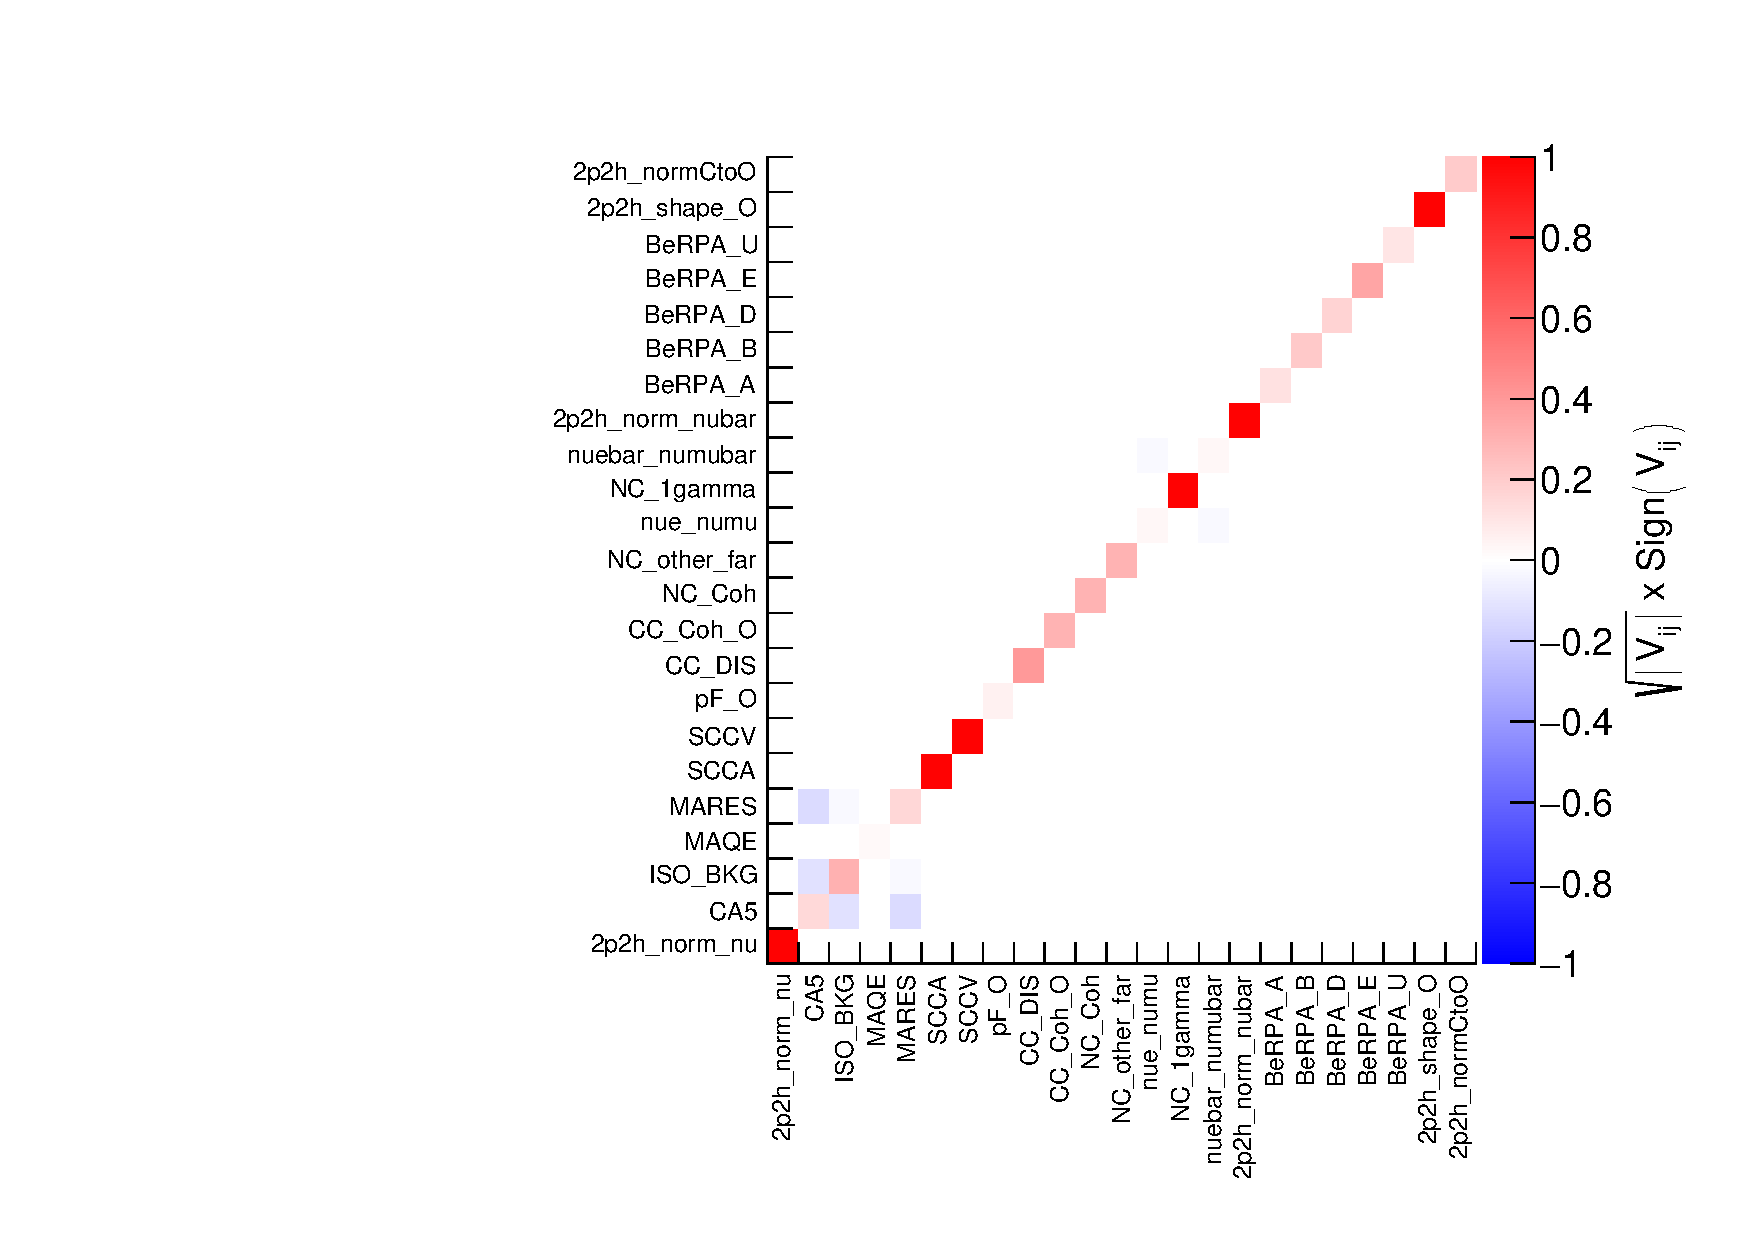
\includegraphics[angle=-90,width=0.9\textwidth]{systematics/banff_xsec_prefit}
	\end{subfigure}
	\begin{subfigure}[b]{0.49\textwidth}
		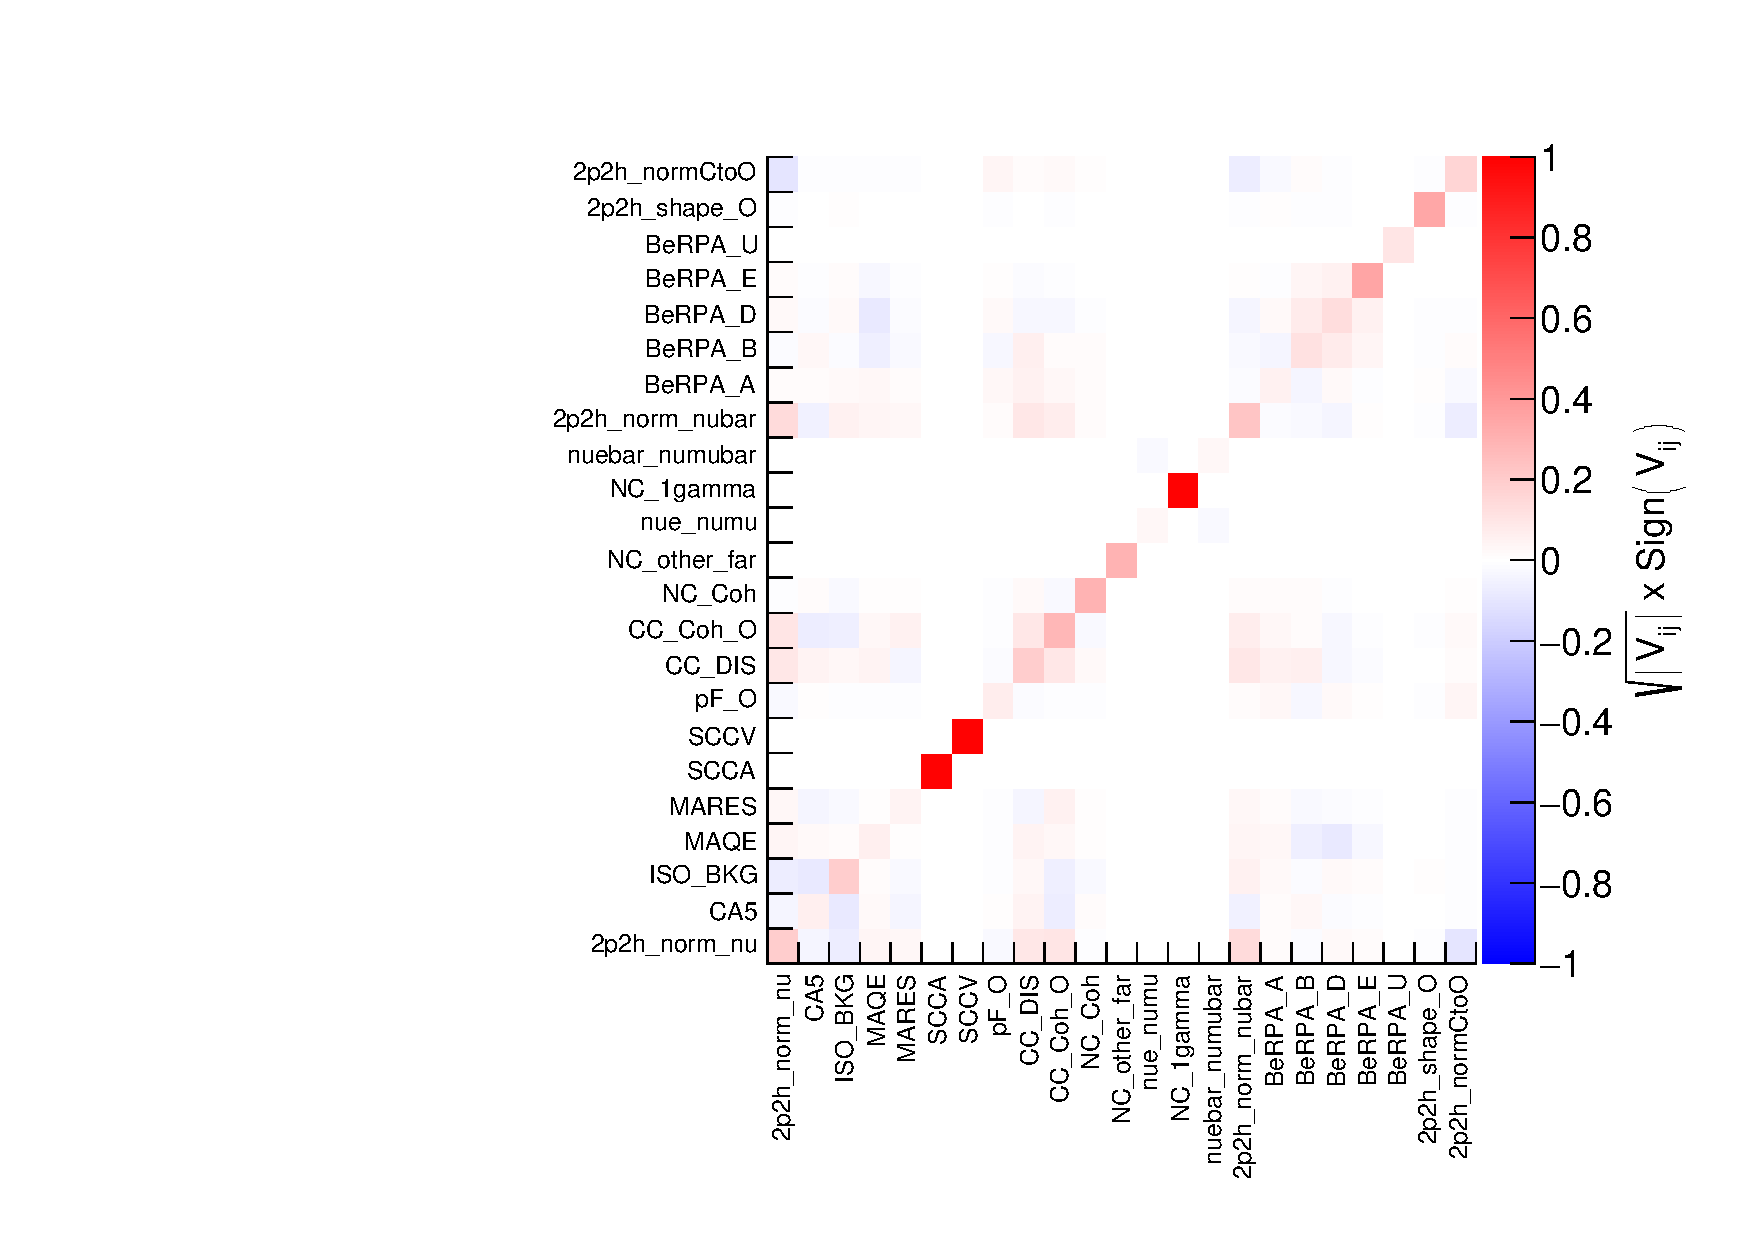
\includegraphics[angle=-90,width=0.9\textwidth]{systematics/banff_xsec_postfit}
	\end{subfigure}
	\caption{The pre-BANFF (left) and post-BANFF (right) cross-section covariance matrix, with the values shown as the sign of the element times the square root of the absolute value of the element.}
\label{fig:xsec_corr}
\end{figure*}

Many of the cross-section parameters are the same as those used in the previous analysis \cite{OurRun17cCC1piJointAnalysis3Flavour}. However, the binding energy for $^{16}$O is no longer included in this analysis and a number of new parameters have been included, see \cref{sec:systematics:2p2h_berpa}. Five of these new parameters (2p2h, BeRPA A, B, D and E) are implemented using cubic splines, details for which can be found in \cite{OurRun17cCC1piJointAnalysis3Flavour}, while one of the new parameters (BeRPA U) is fixed in the analysis.

\subsubsection{Neutrino-nucleus interaction uncertainties}
\label{sec:systematics:2p2h_berpa}
Overall normalisation uncertainties for 2p2h interactions were included in previous analyses, but this analysis includes a 2p2h shape uncertainty (using best-fit value and errors from the BANFF fit) to describe the uncertainty in the cross-section strength between Delta-like, non-Delta-like and interference terms of the 2p2h model, determined by redistributing the cross-section strength of these terms subject to (approximately) maintaining the total 2p2h event rate (see Section 2 of \cite{NewXsecImplementation}). In terms of energy transfer (q0) and three-momentum transfer (q3) kinematics, the distribution of events in this space for neutrino and antineutrino interactions on oxygen are shown in \cref{fig:2p2h_neutrino,fig:2p2h_antineutrino} respectively (see Section 2 of \cite{NewXsecImplementation}).

\begin{figure}
	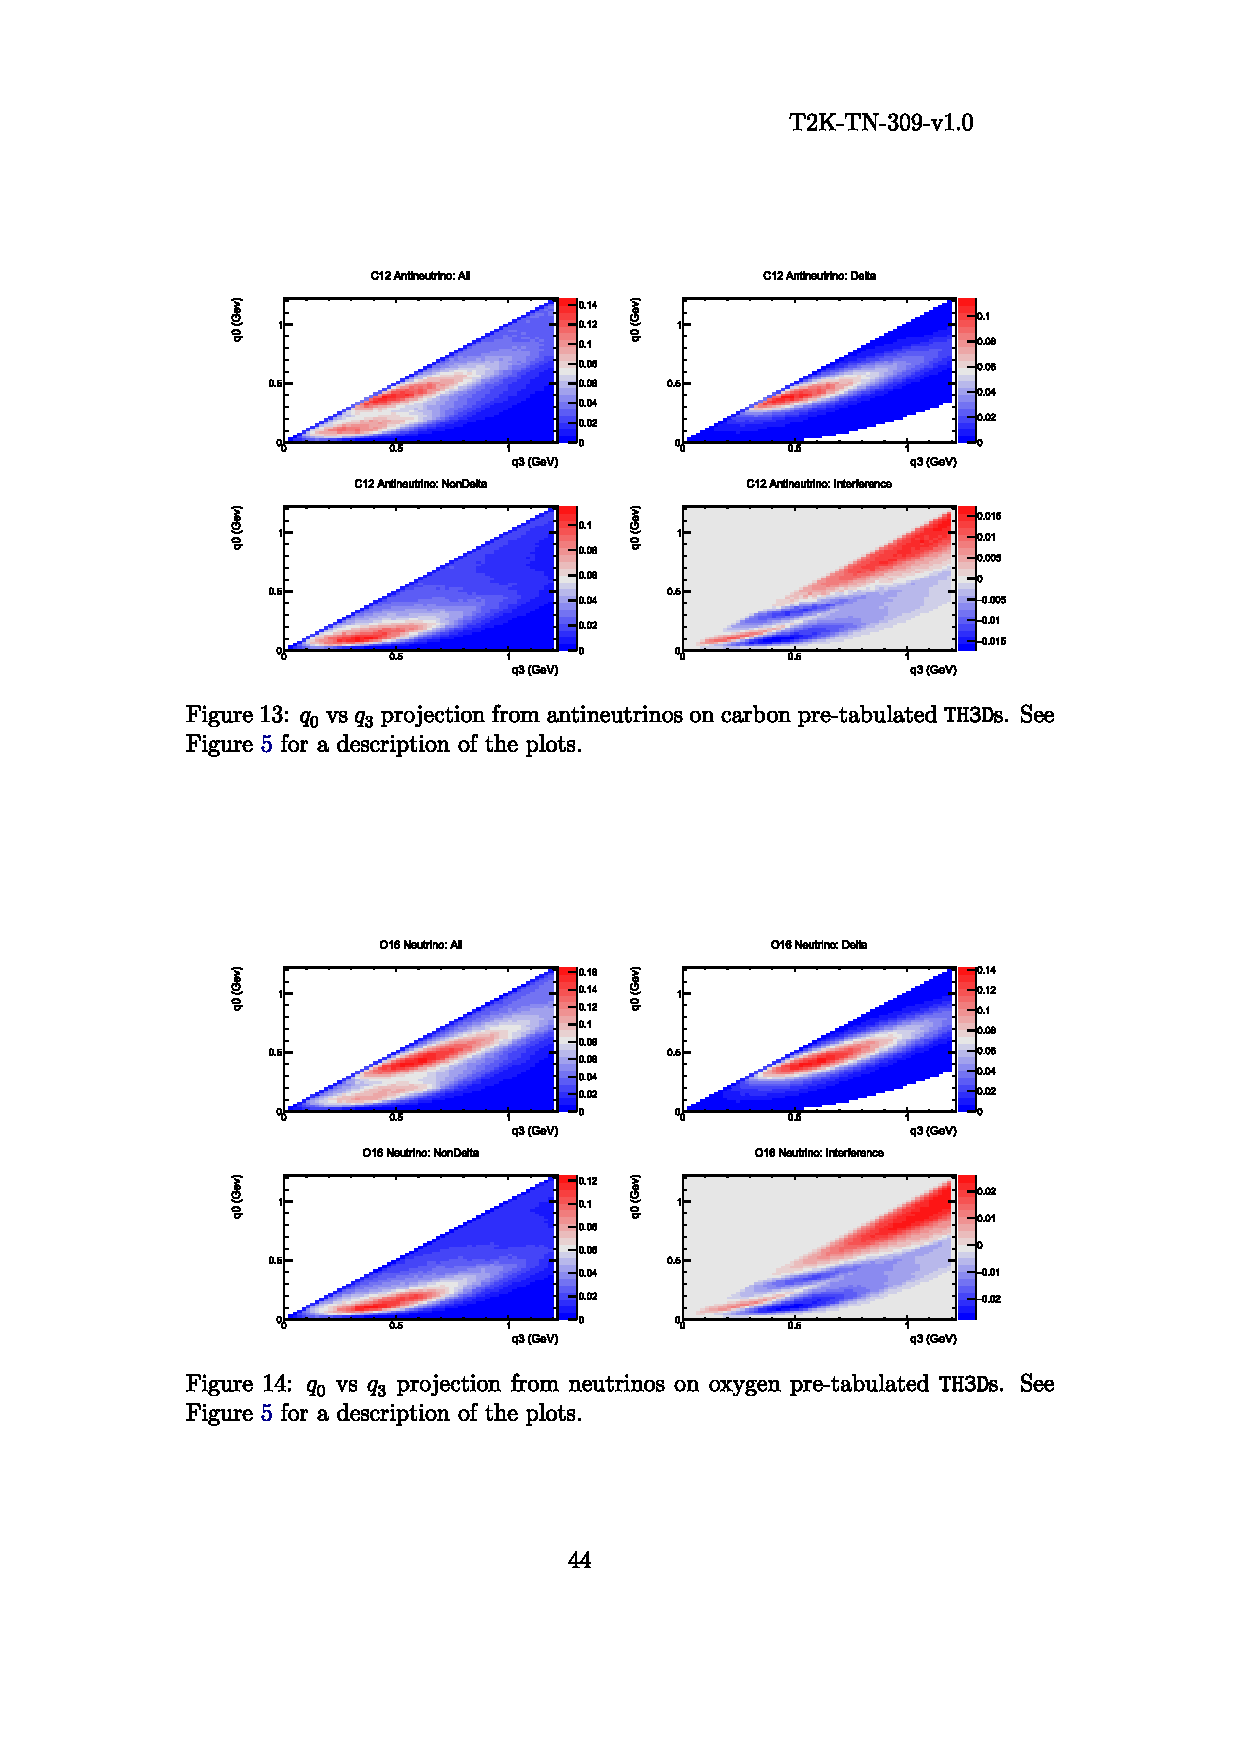
\includegraphics[page=1, trim={2cm 7cm 3cm 15.5cm}, clip, scale=1.0]{systematics/2p2h}
	\caption{Distribution of neutrino events for 2p2h and each 2p2h term in q0-q3 space \cite{NewXsecImplementation}.}
	\label{fig:2p2h_neutrino}
\end{figure}

\begin{figure}
	\includegraphics[page=2, trim={2cm 19cm 3cm 3.5cm}, clip, scale=1.0]{systematics/2p2h}
	\caption{Distribution of antineutrino events for 2p2h and each 2p2h term in q0-q3 space \cite{NewXsecImplementation}.}
	\label{fig:2p2h_antineutrino}
\end{figure}

This analysis also introduces 5 BeRPA parameters (A, B, D, E and U) to describe the collective effects of interactions between neutrinos and nucleons inside nuclei. These effects modify the $Q^2$ dependence of the neutrino-nucleus cross-section and in BeRPA are described by a cubic polynomial transitioning to an exponential above a $Q^2$ threshold, as described in \cite{NIWGUpdate2017}. Neither the 2p2h shape parameter nor the BeRPA parameters apply to interactions on free protons.

\subsection{Super-K efficiencies \& effects of intranuclear and secondary re-interactions (44 parameters)}

The Super-K detector uncertainties include the efficiencies of the fiducial volume and reduction chain, and the OD, ring-counting, PID, momentum and decay-electron cuts. These uncertainties have been evaluated by comparisons between SK-IV atmospheric data and atmospheric neutrino Monte Carlo. Ring counting errors are evaluated using $\nu_\mu$ CCQE, $\nu_\mu$ CCnQE, NC, and $\nu_e$ CC-enriched control samples from atmospheric neutrinos.  The NC PID error is evaluated using a NC-enriched control sample, obtained by not using the PID information during the selection. All the Monte Carlo control samples are fitted simultaneously to the data with a $\chi^2$ function using the selection efficiencies as fit parameters ~\cite{SuperkErrors_numu}~\cite{SuperkErrors_nue}.

Intranuclear final-state interactions (FSI) have significant effects in the T2K energy range and result in event topologies, for scattering from nuclear targets, which are drastically different from those created in neutrino scattering from free nucleons.  Uncertainties due to FSI were estimated by simultaneously varying NEUT parameters that scale interaction probabilities as described in section\ 2 of \cite{NIWGErr}. Uncertainties due to secondary pion interactions (SI) were also evaluated by allowing variations in the interaction probabilities. Details of this are given in \cite{SI}.  Since the same model is used for FSI and SI, it is possible to evaluate the uncertainties in both FSI and SI simultaneously. Details of this procedure are described in section\ 8 of \cite{NEUTnuclear}.

A list of the Super-K parameters and their errors can be found in \cref{tab:sys_sk_err}. We consider the Super-K detector efficiency and FSI+SI+PN systematics together, adding their covariance matrices linearly and evaluating the effects of these uncertainties using the Cholesky method. Details of all parameters can be found in \cite{OurRun17cCC1piJointAnalysis3Flavour}.

\begin{table}
	\begin{adjustbox}{width=\textwidth, totalheight=\textheight, keepaspectratio}
		\begin{tabular} { | c | c | c | c |  }
\hline 
Index & Parameter & Description & $1\sigma$ fractional error\\
\hline
0 & $f_{0; t, r}^{SK+FSI}$ & SKDet + FSI/SI  0; Ereco range 0.00 - 0.40 GeV; numu/numubar CCQE (1Rmu) & 0.009\\ 
1 & $f_{1; t, r}^{SK+FSI}$ & SKDet + FSI/SI  1; Ereco range 0.40 - 1.10 GeV; numu/numubar CCQE (1Rmu) & 0.007\\ 
2 & $f_{2; t, r}^{SK+FSI}$ & SKDet + FSI/SI  2; Ereco range 1.10 - 30.00 GeV; numu/numubar CCQE (1Rmu) & 0.007\\ 
3 & $f_{3; t, r}^{SK+FSI}$ & SKDet + FSI/SI  3; Ereco range 0.00 - 30.00 GeV; numu/numubar CCnQE (1Rmu) & 0.169\\ 
4 & $f_{4; t, r}^{SK+FSI}$ & SKDet + FSI/SI  4; Ereco range 0.00 - 30.00 GeV; nue/nuebar/signue CC (1Rmu) & 1.005\\ 
5 & $f_{5; t, r}^{SK+FSI}$ & SKDet + FSI/SI  5; Ereco range 0.00 - 30.00 GeV; all NC (1Rmu) & 0.658\\ 
6 & $f_{6; t, r}^{SK+FSI}$ & SKDet + FSI/SI  6; Ereco range 0.00 - 0.35 GeV; oscillated nue CC (1Re) & 0.181\\ 
7 & $f_{7; t, r}^{SK+FSI}$ & SKDet + FSI/SI  7; Ereco range 0.35 - 0.80 GeV; oscillated nue CC (1Re) & 0.036\\ 
8 & $f_{8; t, r}^{SK+FSI}$ & SKDet + FSI/SI  8; Ereco range 0.80 - 1.25 GeV; oscillated nue CC (1Re) & 0.042\\ 
9 & $f_{9; t, r}^{SK+FSI}$ & SKDet + FSI/SI  9; Ereco range 0.00 - 0.35 GeV; numu/numubar CC (1Re) & 0.300\\ 
10 & $f_{10; t, r}^{SK+FSI}$ & SKDet + FSI/SI 10; Ereco range 0.35 - 0.80 GeV; numu/numubar CC (1Re) & 0.321\\ 
11 & $f_{11; t, r}^{SK+FSI}$ & SKDet + FSI/SI 11; Ereco range 0.80 - 1.25 GeV; numu/numubar CC (1Re) & 0.393\\ 
12 & $f_{12; t, r}^{SK+FSI}$ & SKDet + FSI/SI 12; Ereco range 0.00 - 0.35 GeV; nue/nuebar CC (1Re) & 0.135\\ 
13 & $f_{13; t, r}^{SK+FSI}$ & SKDet + FSI/SI 13; Ereco range 0.35 - 0.80 GeV; nue/nuebar CC (1Re) & 0.070\\ 
14 & $f_{14; t, r}^{SK+FSI}$ & SKDet + FSI/SI 14; Ereco range 0.80 - 1.25 GeV; nue/nuebar CC (1Re) & 0.077\\ 
15 & $f_{15; t, r}^{SK+FSI}$ & SKDet + FSI/SI 15; Ereco range 0.00 - 0.35 GeV; all NC (1Re) & 0.194\\ 
16 & $f_{16; t, r}^{SK+FSI}$ & SKDet + FSI/SI 16; Ereco range 0.35 - 0.80 GeV; all NC (1Re) & 0.181\\ 
17 & $f_{17; t, r}^{SK+FSI}$ & SKDet + FSI/SI 17; Ereco range 0.80 - 1.25 GeV; all NC (1Re) & 0.472\\ 
18 & $f_{0; t, r}^{SK+FSI}RHC$ & SKDet + FSI/SI  0; Ereco range 0.00 - 0.40 GeV; numu/numubar CCQE (1Rmu); RHC & 0.009\\ 
19 & $f_{1; t, r}^{SK+FSI}RHC$ & SKDet + FSI/SI  1; Ereco range 0.40 - 1.10 GeV; numu/numubar CCQE (1Rmu); RHC & 0.007\\ 
20 & $f_{2; t, r}^{SK+FSI}RHC$ & SKDet + FSI/SI  2; Ereco range 1.10 - 30.00 GeV; numu/numubar CCQE (1Rmu); RHC & 0.007\\ 
21 & $f_{3; t, r}^{SK+FSI}RHC$ & SKDet + FSI/SI  3; Ereco range 0.00 - 30.00 GeV; numu/numubar CCnQE (1Rmu); RHC & 0.130\\ 
22 & $f_{4; t, r}^{SK+FSI}RHC$ & SKDet + FSI/SI  4; Ereco range 0.00 - 30.00 GeV; nue/nuebar/signue CC (1Rmu); RHC & 1.005\\ 
23 & $f_{5; t, r}^{SK+FSI}RHC$ & SKDet + FSI/SI  5; Ereco range 0.00 - 30.00 GeV; all NC (1Rmu); RHC & 0.657\\ 
24 & $f_{6; t, r}^{SK+FSI}RHC$ & SKDet + FSI/SI  6; Ereco range 0.00 - 0.35 GeV; oscillated nue CC (1Re); RHC & 0.108\\ 
25 & $f_{7; t, r}^{SK+FSI}RHC$ & SKDet + FSI/SI  7; Ereco range 0.35 - 0.80 GeV; oscillated nue CC (1Re); RHC & 0.036\\ 
26 & $f_{8; t, r}^{SK+FSI}RHC$ & SKDet + FSI/SI  8; Ereco range 0.80 - 1.25 GeV; oscillated nue CC (1Re); RHC & 0.057\\ 
27 & $f_{9; t, r}^{SK+FSI}RHC$ & SKDet + FSI/SI  9; Ereco range 0.00 - 0.35 GeV; numu/numubar CC (1Re); RHC & 0.349\\ 
28 & $f_{10; t, r}^{SK+FSI}RHC$ & SKDet + FSI/SI 10; Ereco range 0.35 - 0.80 GeV; numu/numubar CC (1Re); RHC & 0.342\\ 
29 & $f_{11; t, r}^{SK+FSI}RHC$ & SKDet + FSI/SI 11; Ereco range 0.80 - 1.25 GeV; numu/numubar CC (1Re); RHC & 0.417\\ 
30 & $f_{12; t, r}^{SK+FSI}RHC$ & SKDet + FSI/SI 12; Ereco range 0.00 - 0.35 GeV; nue/nuebar CC (1Re); RHC & 0.085\\ 
31 & $f_{13; t, r}^{SK+FSI}RHC$ & SKDet + FSI/SI 13; Ereco range 0.35 - 0.80 GeV; nue/nuebar CC (1Re); RHC & 0.056\\ 
32 & $f_{14; t, r}^{SK+FSI}RHC$ & SKDet + FSI/SI 14; Ereco range 0.80 - 1.25 GeV; nue/nuebar CC (1Re); RHC & 0.078\\ 
33 & $f_{15; t, r}^{SK+FSI}RHC$ & SKDet + FSI/SI 15; Ereco range 0.00 - 0.35 GeV; all NC (1Re); RHC & 0.214\\ 
34 & $f_{16; t, r}^{SK+FSI}RHC$ & SKDet + FSI/SI 16; Ereco range 0.35 - 0.80 GeV; all NC (1Re); RHC & 0.191\\ 
35 & $f_{17; t, r}^{SK+FSI}RHC$ & SKDet + FSI/SI 17; Ereco range 0.80 - 1.25 GeV; all NC (1Re); RHC & 0.465\\ 
36 & $f_{0; t, r}^{SK+FSI}MultiRing$ & SKDet + FSI/SI  0; Ereco range 0.30 - 0.80 GeV; oscillated nue CC (MultiRe); MultiRing & 0.249\\ 
37 & $f_{1; t, r}^{SK+FSI}MultiRing$ & SKDet + FSI/SI  1; Ereco range 0.80 - 1.25 GeV; oscillated nue CC (MultiRe); MultiRing & 0.215\\ 
38 & $f_{2; t, r}^{SK+FSI}MultiRing$ & SKDet + FSI/SI  2; Ereco range 0.30 - 0.80 GeV; numu/numubar CC (MultiRe); MultiRing & 0.507\\ 
39 & $f_{3; t, r}^{SK+FSI}MultiRing$ & SKDet + FSI/SI  3; Ereco range 0.80 - 1.25 GeV; numu/numubar CC (MultiRe); MultiRing & 0.236\\ 
40 & $f_{4; t, r}^{SK+FSI}MultiRing$ & SKDet + FSI/SI  4; Ereco range 0.30 - 0.80 GeV; nue/nuebar CC (MultiRe); MultiRing & 0.244\\ 
41 & $f_{5; t, r}^{SK+FSI}MultiRing$ & SKDet + FSI/SI  5; Ereco range 0.80 - 1.25 GeV; nue/nuebar CC (MultiRe); MultiRing & 0.235\\ 
42 & $f_{6; t, r}^{SK+FSI}MultiRing$ & SKDet + FSI/SI  6; Ereco range 0.30 - 0.80 GeV; all NC (MultiRe); MultiRing & 0.983\\ 
43 & $f_{7; t, r}^{SK+FSI}MultiRing$ & SKDet + FSI/SI  7; Ereco range 0.80 - 1.25 GeV; all NC (MultiRe); MultiRing & 0.524\\ 
44 & $f_{E; r}^{SK}$ & SK energy scale & 0.024\\ 

\hline

\end{tabular}
	\end{adjustbox}
	\caption{Summary of SK detector + FSI + SI + PN systematics included in the VALOR joint fit analysis.}
	\label{tab:sys_sk_err}
\end{table}

\subsection{Super-K energy scale (1 parameter)}

The systematic parameter $f_{E; r}^{SK}$ is included to estimate the effects of uncertainty in the Super-K reconstructed energy scale.  This uncertainty is estimated to be 2.4\% \cite{SuperkEScale2013}; its effects are calculated by scaling the bin edges of the MC templates and, assuming uniform distribution of events within the bins, calculating the number of events gained from/lost to other bins (including bins that are not immediately adjacent). This systematic is applied after all other systematics have been applied, because it affects reconstructed rather than true energy, does not commute with spline-based systematics, which are generated without consideration of energy scale variation and also does not commute with the other Super-K systematics, which are determined from data without any energy scale variation.

\subsection{Oscillation parameters and mass hierarchy (7 parameters)}

The 3-flavour oscillation probability is used.  All the nuisance oscillation parameters, i.e. those parameters which are not shown in a given contour, are marginalised except the mass hierarchy which is fixed to either normal or inverted hierarchy.

For $\sin^2 \theta_{13}$ two different priors can be used, depending on whether the reactor constraint is applied, denoted as ``reactors", when applied and ``T2K only" when not applied.

\begin{table}
	\centering
	\begin{tabular}{| c | c | c | c |}
 	\hline
Parameter(s)	& Prior		& Range    \\
\hline
$\sin^{2}\theta_{23}$	&  uniform 	& $[0.3; 0.7]$      \\
$\sin^{2} 2 \theta_{13}$ ($\sin^{2} \theta_{13}$) reactors		&  gaussian 		& $0.0857 \pm 0.0046$ 	\\
$\sin^{2} 2 \theta_{13}$ ($\sin^{2} \theta_{13}$) T2K only	   	&  uniform		& $[0; 0.4]$ 	\\
$\sin^{2} 2 \theta_{12}$  								&  gaussian 		& $0.846 \pm 0.021$ \\
$|\Delta m^{2}_{32}|$ (NH) / $|\Delta m^{2}_{13}|$ (IH)      		&  uniform		& $ [2.3; 2.7] \times 10^{-3}~\mbox{eV}^2/\mbox{c}^4$		 \\
$\Delta m^{2}_{21}$      								&  gaussian 		& $(7.53 \pm 0.18) \times 10^{-5}~\mbox{eV}^2/\mbox{c}^4$		\\
$\delta_{CP}$                                               				&  uniform 	& $[-\pi; +\pi]$ \\
Mass Hierarchy										&  fixed 		& NH or IH \\  
\hline
\end{tabular}
\caption{
Treatment of the oscillation parameters in the $\nu/\bar{\nu}$ joint analysis. All the gaussian priors are from \cite{pdg_2014}. The parameter $\sin^{2} 2 \theta_{13}$ can be constrained with the measurement of reactor experiments using the gaussian prior, otherwise a uniform prior is used and the measurement relies only on the T2K data. The nominal values of $\sin^2 2 \theta_{13}$, $\sin^2 2 \theta_{12}$ and $\Delta m^2_{21}$ are from \cite{pdg_2014}, while all the other oscillation parameter values corresponds to the most probable values obtained by the Bayesian analysis on the T2K run 1-4 neutrino mode data \cite{T2KLongPaper}. The mass hierarchy is not marginalised but fixed to either NH or IH.
}
\label{tab:osc_param_priors}
\end{table}

\subsection{Systematic error on Super-K predictions}
\label{sec:systematics:errortables}

The effect of each category of systematic parameter on the expected event rate for Super-K sample is given in \crefrange{tab:sk_errors_1Rmu}{tab:sk_errors_MultiRe} (details of per-sample event rates for $1\sigma$ and $3\sigma$ variations of each independent systematic parameter can be found in \cref{app:sysvar}). The mean and RMS of 10000 throws of the respective systematics (with correlations taken into account) is computed for each sample and in the case of pre-BANFF and post-BANFF errors. When not measuring the effect of oscillation parameters variations, the oscillation parameters are fixed at Asimov A values (see \cref{sec:asimov_definition}).

For the measurement of $\delta_{CP}$ it is important to understand the effect of the systematic uncertainties on the ratio of the number of events between neutrino and antineutrino mode samples. If correlations do not reproduce the physics correctly, a fake asymmetry between neutrino and antineutrino oscillations can be seen. Furthermore, if correlations exist but are not taken into account, the measurement of $\delta_{CP}$ could be biased. The true value of $\delta_{CP}$ determines whether correlations or anti-correlations between systematic parameters have the greatest effect in hiding any oscillation asymmetry. In particular, if true $\delta_{CP} = \pm \pi/2$ then anti-correlation in the $e$-like samples could hide any oscillation asymmetry. Alternatively, in the case that true $\delta_{CP} \sim 0$ it is uncorrelated parameters that reduce the sensitivity to $\delta_{CP}$. The uncertainties on the ratios between neutrino and antineutrino mode events due to the systematic parameters are shown in \cref{tab:sk_errors_summary}. The most critical systematic parameters are $\sigma_{\nu_e}$ and $\sigma_{\bar{\nu}_e}$ which are applied respectively to $\nu_e$ and $\bar{\nu}_e$ events. Their fractional error from the BANFF covariance matrix is 2.83\% (see \cref{tab:sys_xsec_err}) and they are partially anti-correlated with non-diagonal elements in the covariance matrix of -0.0004.

It can be seen in \crefrange{tab:sk_errors_1Rmu}{tab:sk_errors_MultiRe} (\Cref{app:sk_errors}) that the reduction in the error on flux and constrained cross-section systematics achieved through the BANFF fit reduces the fractional error due to all systematics from $\sim 14\%$ to $\sim 4\%$ and $\sim 11\%$ to $\sim 3\%$ in the neutrino- and antineutrino-mode $\mu$-like samples respectively, from $\sim 16\%$ to $\sim 7\%$ and $\sim 13\%$ to $\sim 8\%$ in the neutrino- and antineutrino-mode $e$-like samples respectively, and from $\sim 25\%$ to $\sim 22\%$ in the \nueCConepi{}-like sample. A summary of the effects of the systematic errors is given in \cref{tab:sk_errors_summary}.

\begin{table}[H]
	\centering
	\begin{tabular}{|l||l|l||l|l|l|l|l|}
		\hline
		& \multicolumn{2}{c||}{\textbf{1-Ring $\mu$}} & \multicolumn{4}{c|}{\textbf{1-Ring $e$}} \\ \hline
		Error source & FHC & RHC & FHC & RHC & FHC 1 d.e. & FHC/RHC \\ \hline\hline
		SK Detector & 1.86 & 1.51 & 3.03 & 4.22 & 16.69 & 1.60 \\ \hline
		SK FSI+SI+PN & 2.20 & 1.98 & 3.01 & 2.31 & 11.43 & 1.57 \\ \hline
		Flux + Xsec constrained & 3.22 & 2.72 & 3.22 & 2.88 & 4.05 & 2.50 \\ \hline
		$\sigma(\nu_e)/\sigma(\bar{\nu}_e)$ & 0.00 & 0.00 & 2.63 & 1.46 & 2.62 & 3.03 \\ \hline
		NC1$\gamma$ & 0.00 & 0.00 & 1.08 & 2.59 & 0.33 & 1.49 \\ \hline
		NC Other & 0.25 & 0.25 & 0.14 & 0.33 & 0.98 & 0.18 \\ \hline
		Osc & 0.04 & 0.03 & 3.86 & 3.60 & 3.78 & 0.79 \\ \hline\hline
		All Systematics & 4.40 & 3.76 & 6.10 & 6.51 & 20.94 & 4.77 \\ \hline
		All with osc & 4.40 & 3.76 & 7.27 & 7.44 & 21.24 & 4.85 \\ \hline
	\end{tabular}
	\caption
	{
	Percentage error on event rate by error source and sample. Final column is the percentage error on the ratio of FHC/RHC events in the one-ring $e$ sample.
	}
	\label{tab:sk_errors_summary}
\end{table}


The error envelopes corresponding to \crefrange{tab:sk_errors_1Rmu}{tab:sk_errors_MultiRe} are shown in \crefrange{fig:sk_envelopes_all}{fig:sk_envelopes_xsec_ncoth_b}. These error envelopes are determined by performing \num{1e4} correlated throws of the systematic parameter group under consideration and plotting the mean and Gaussian $1\sigma$ error resulting.

\begin{figure*}
	\center
	\begin{subfigure}[b]{0.49\textwidth}
		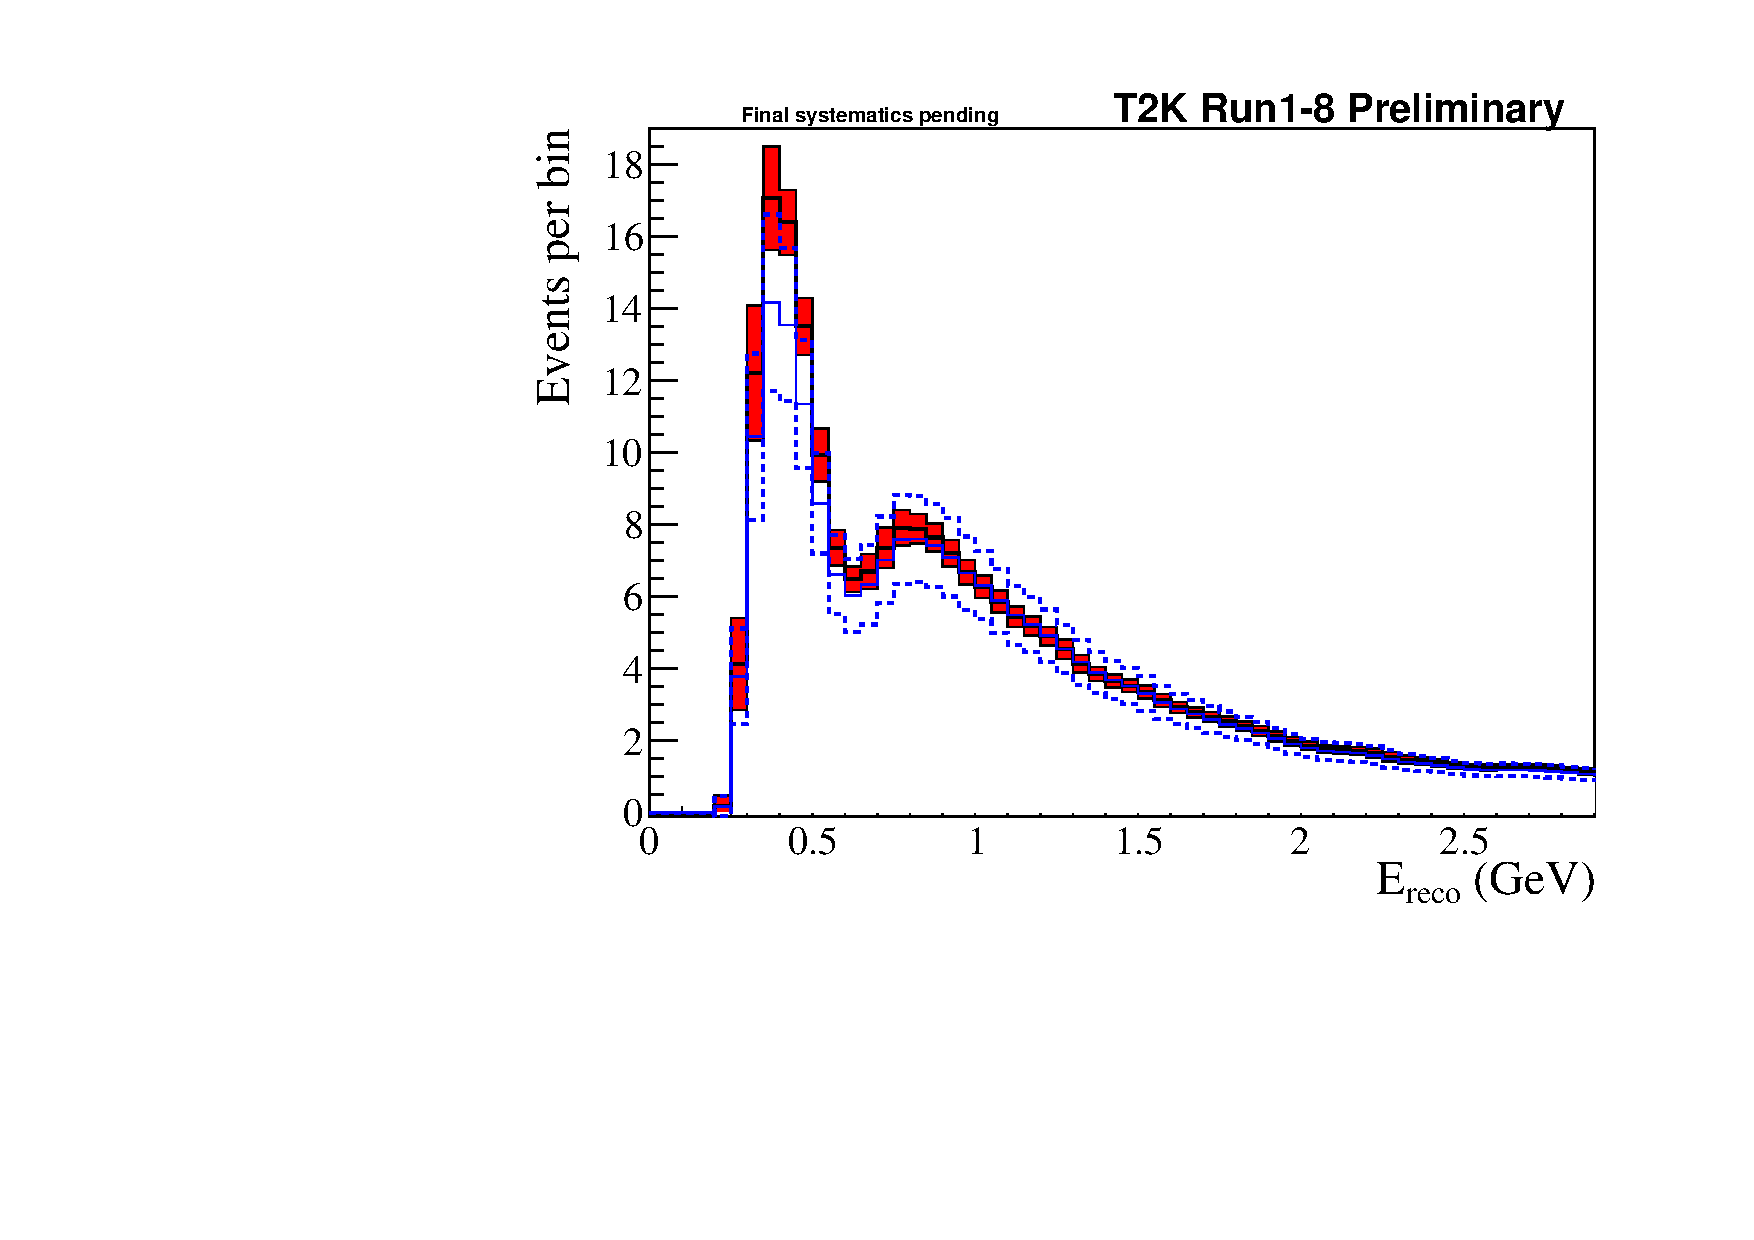
\includegraphics[width=0.9\textwidth]{systematics/envelopes/sk_errors/sk_error_table_1Rmu_all_envelope}
		\caption{Muon-like, neutrino mode}
	\end{subfigure}
	\begin{subfigure}[b]{0.49\textwidth}
		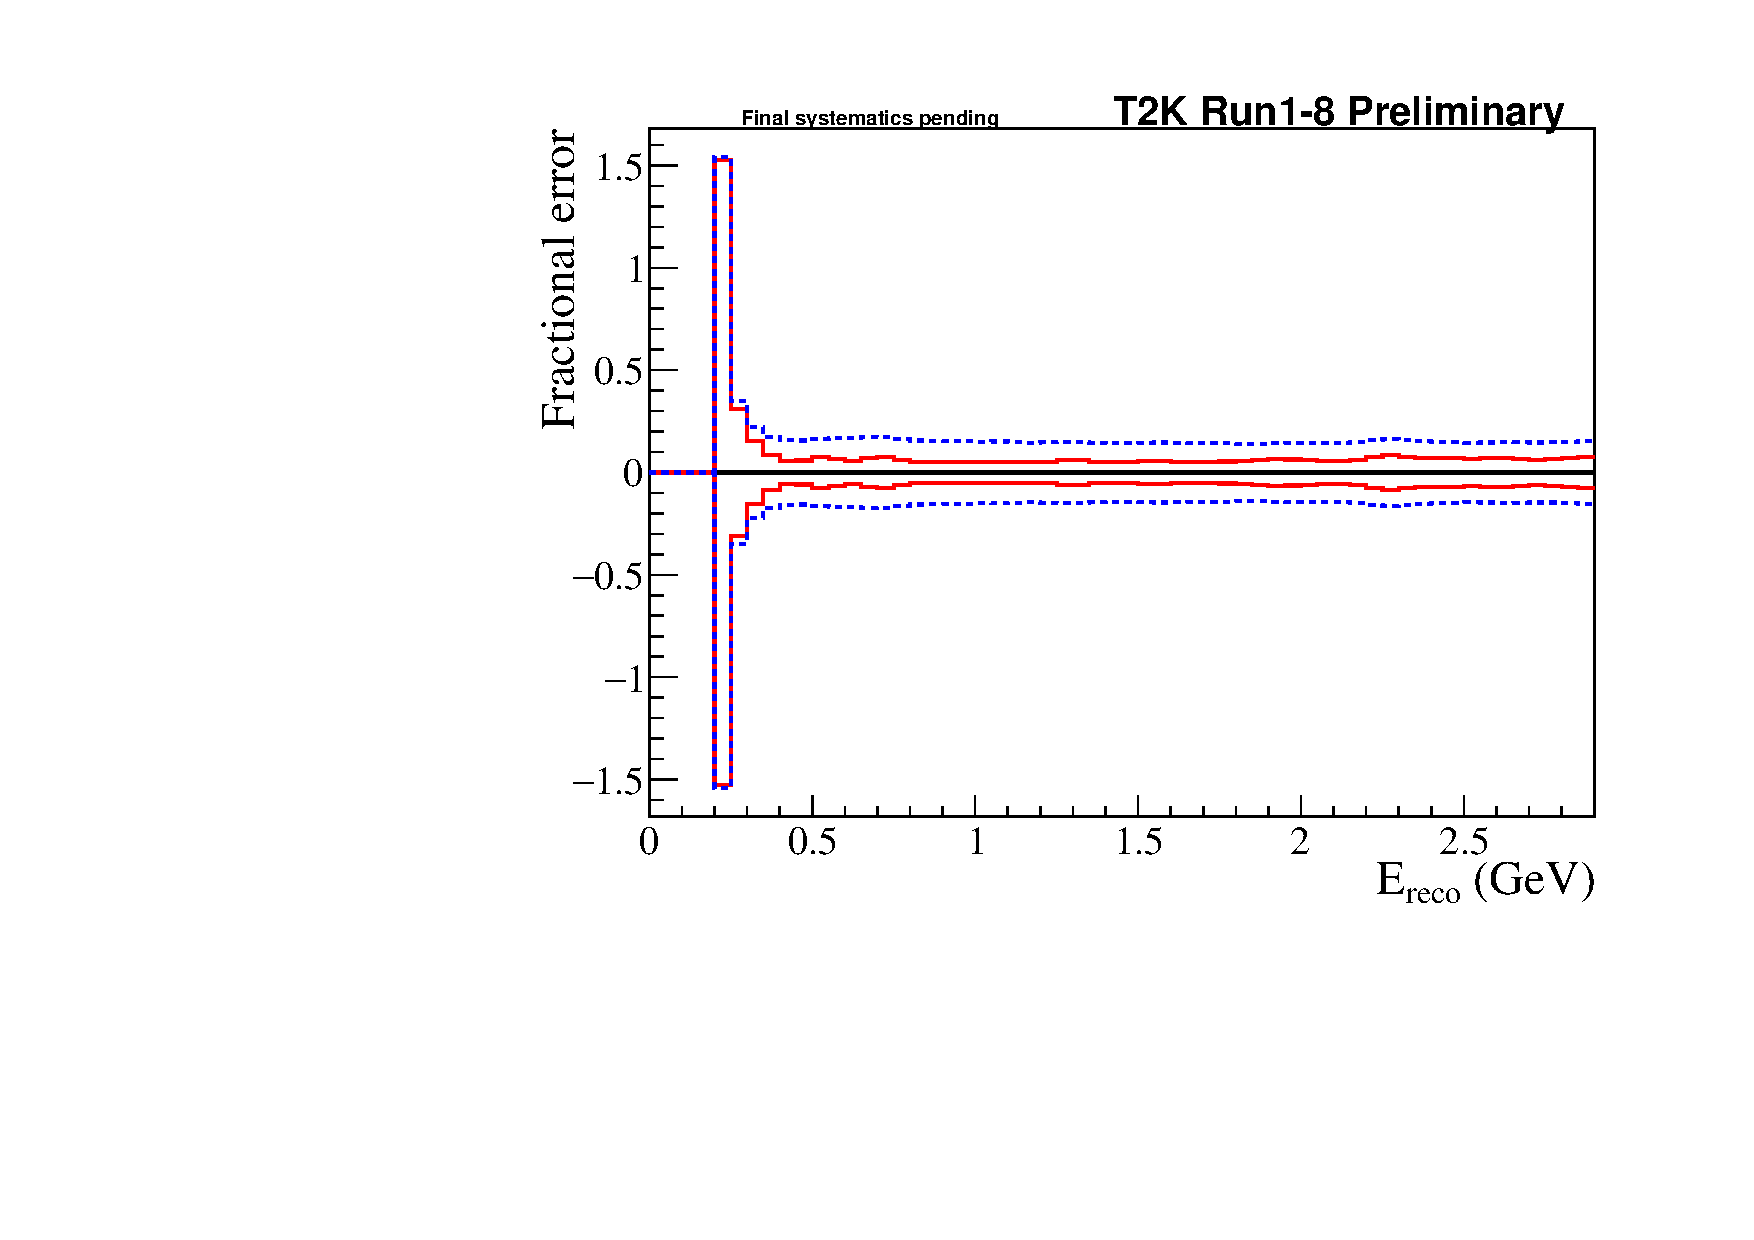
\includegraphics[width=0.9\textwidth]{systematics/envelopes/sk_errors/sk_error_table_1Rmu_all_envelope_fractional}
		\caption{Muon-like, neutrino mode}
	\end{subfigure}
	\begin{subfigure}[b]{0.49\textwidth}
		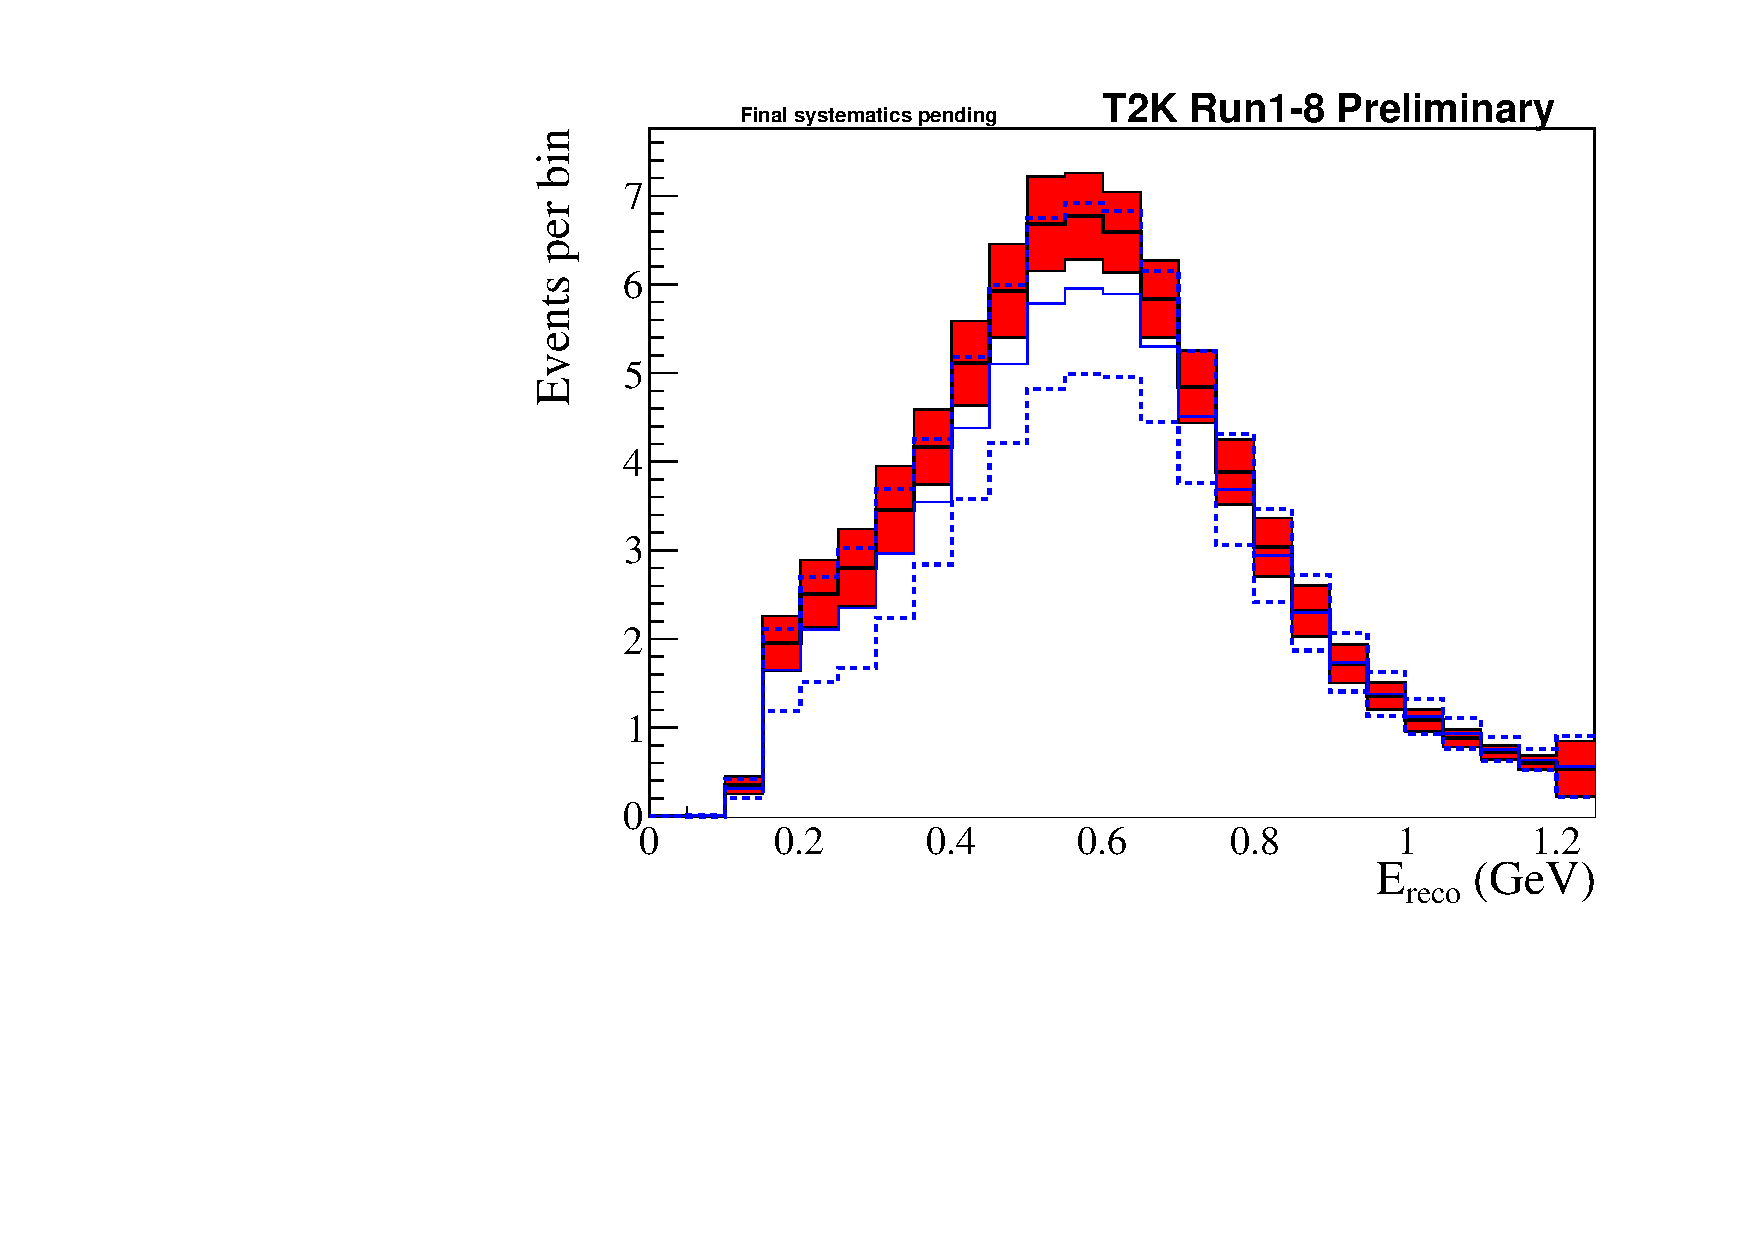
\includegraphics[width=0.9\textwidth]{systematics/envelopes/sk_errors/sk_error_table_1Re_all_envelope}
		\caption{Electron-like, neutrino mode}
	\end{subfigure}
	\begin{subfigure}[b]{0.49\textwidth}
		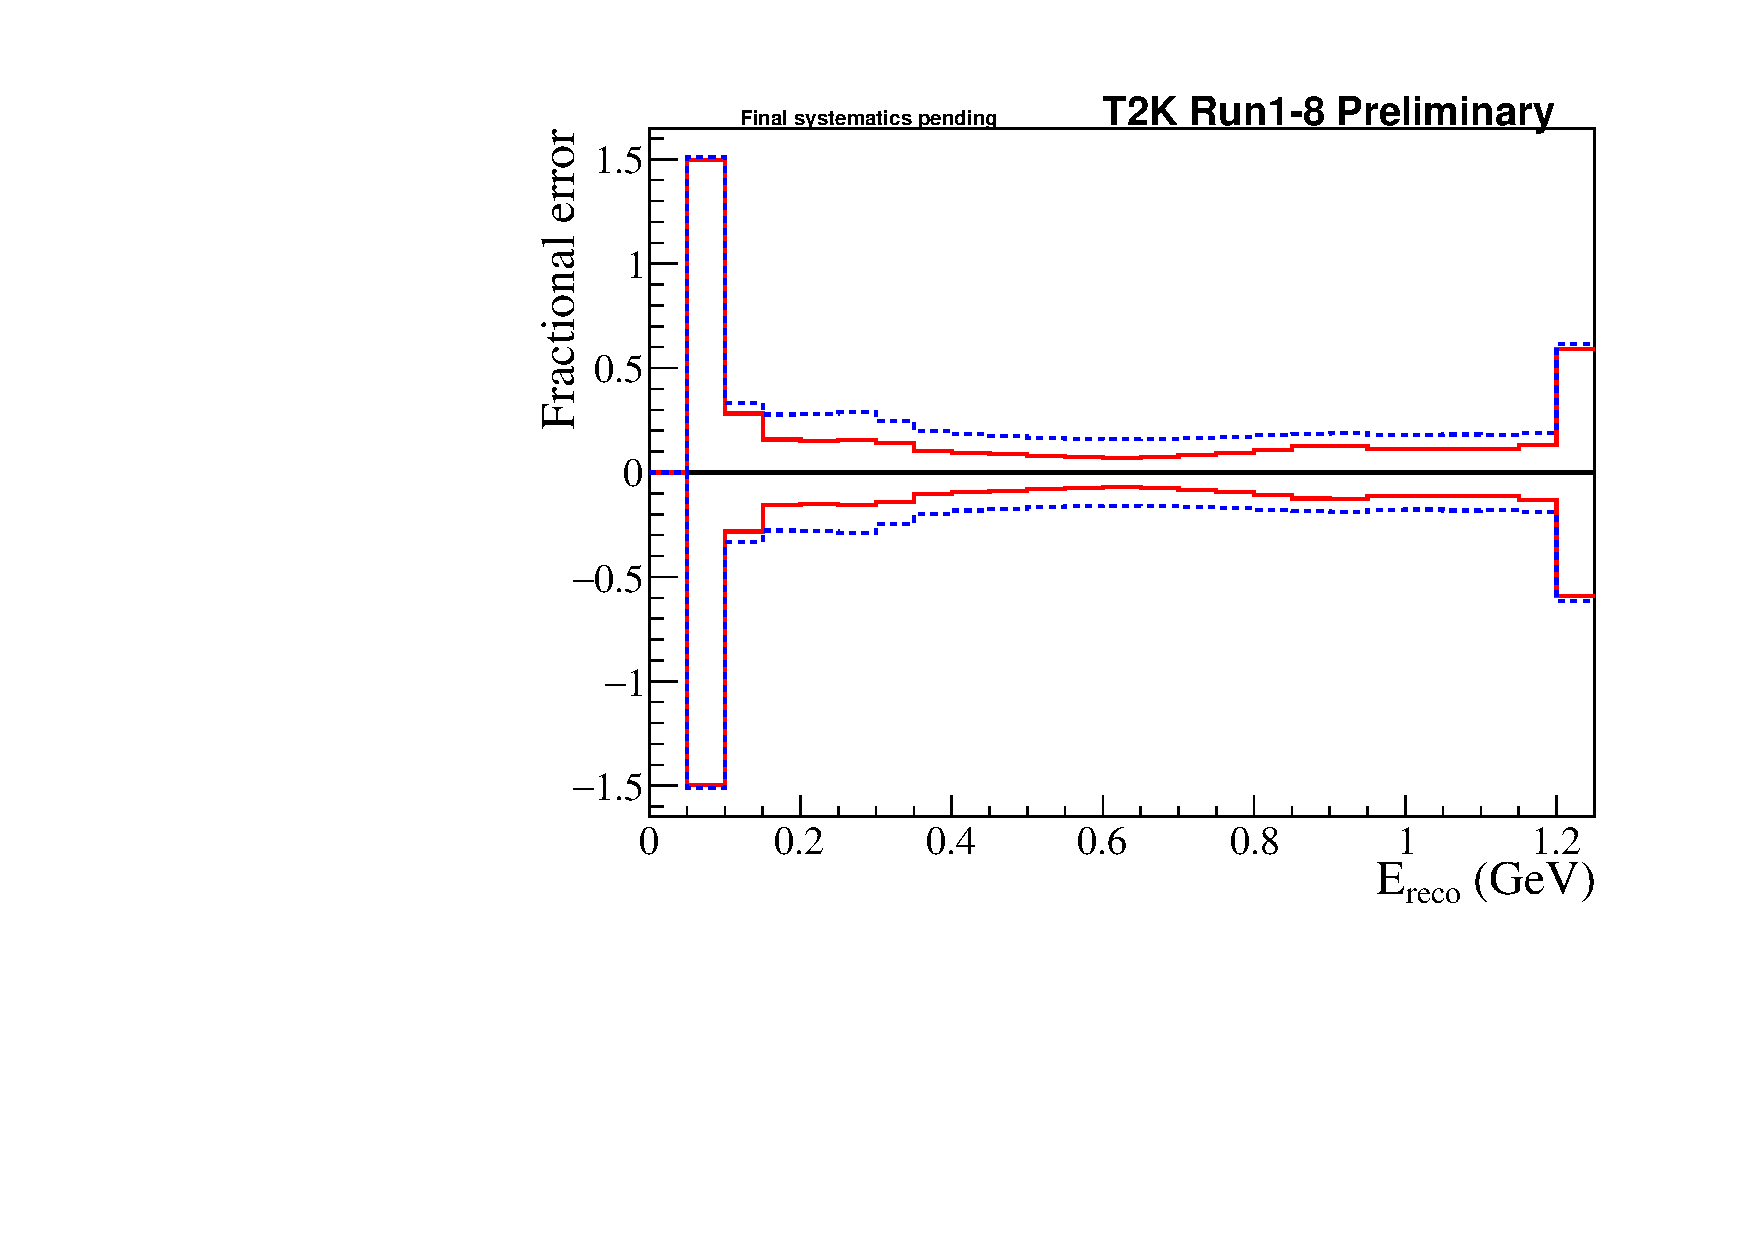
\includegraphics[width=0.9\textwidth]{systematics/envelopes/sk_errors/sk_error_table_1Re_all_envelope_fractional}
		\caption{Electron-like, neutrino mode}
	\end{subfigure}
	\begin{subfigure}[b]{0.49\textwidth}
		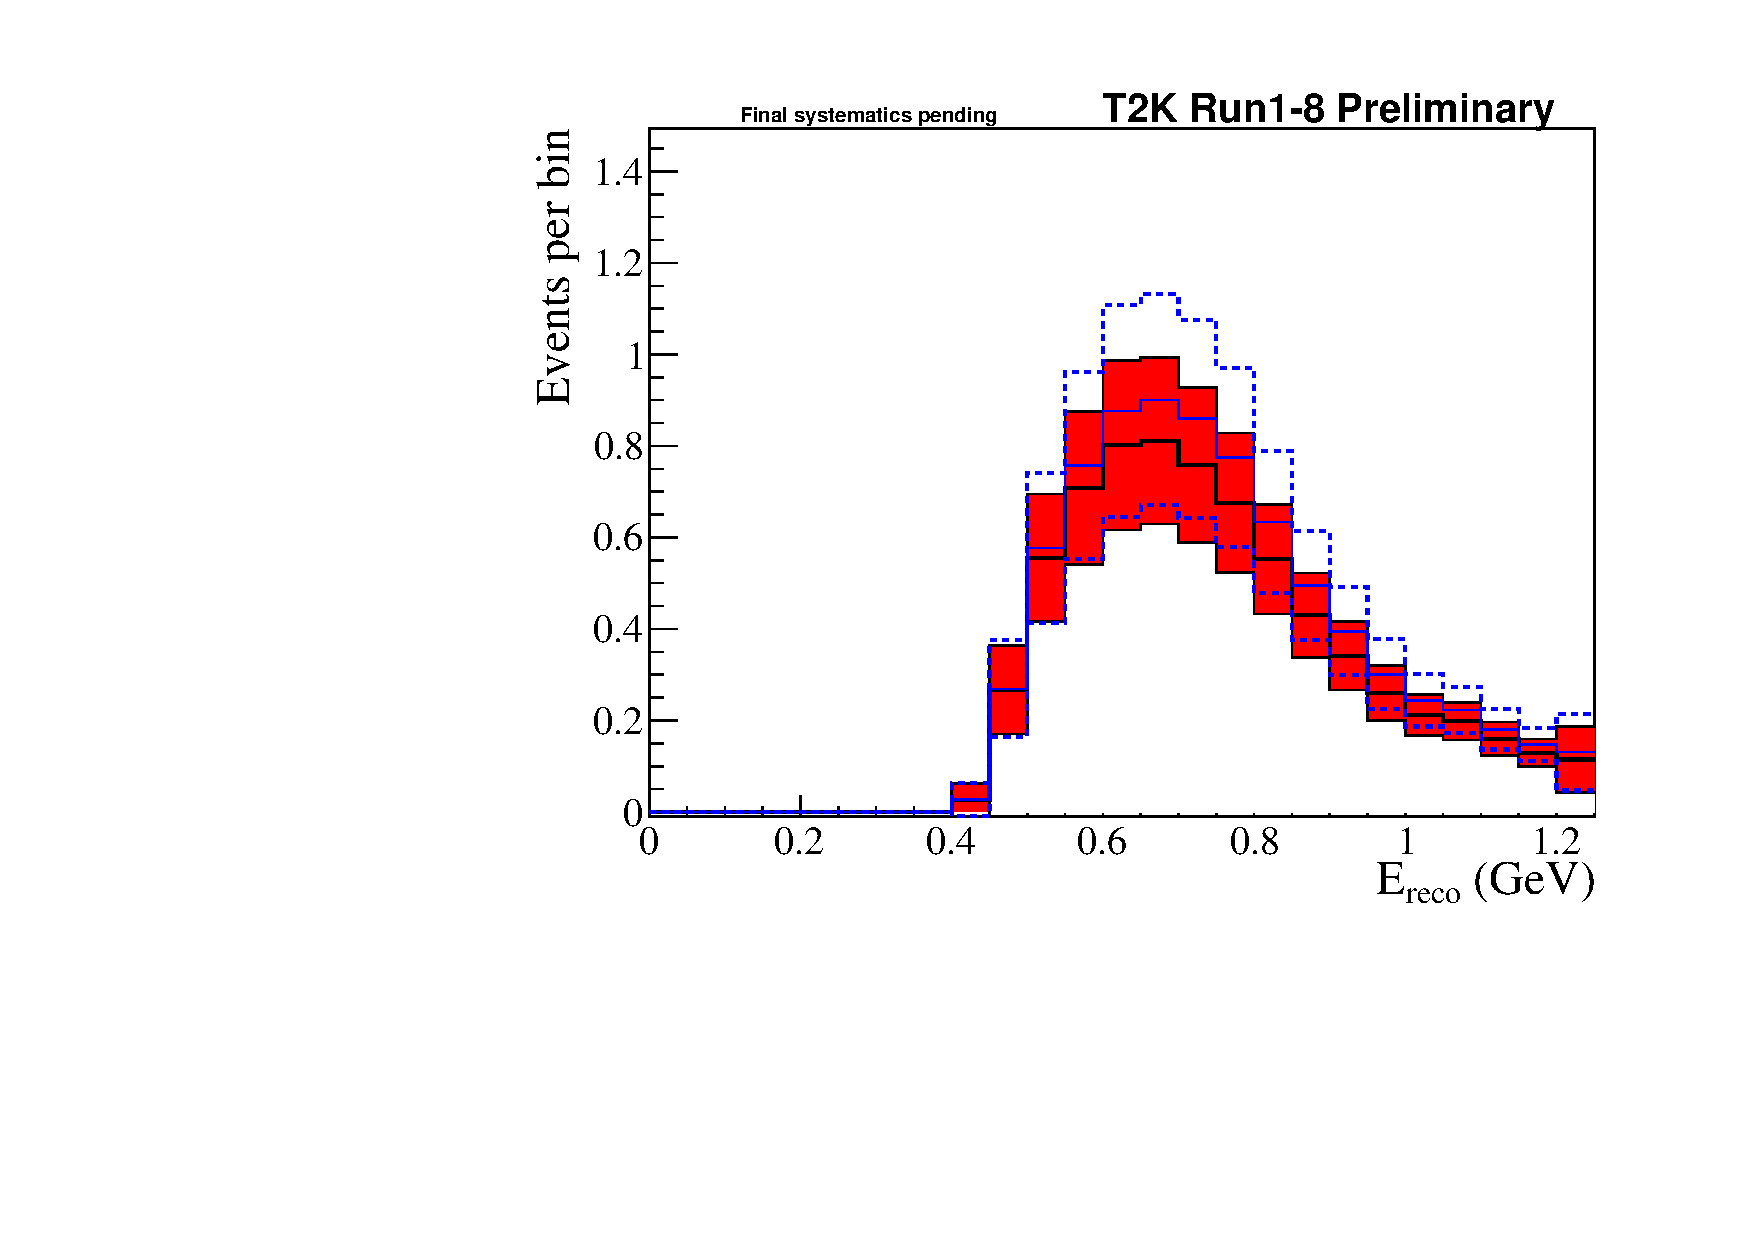
\includegraphics[width=0.9\textwidth]{systematics/envelopes/sk_errors/sk_error_table_MultiRe_all_envelope}
		\caption{\nueCConepi-like, neutrino mode}
	\end{subfigure}
	\begin{subfigure}[b]{0.49\textwidth}
		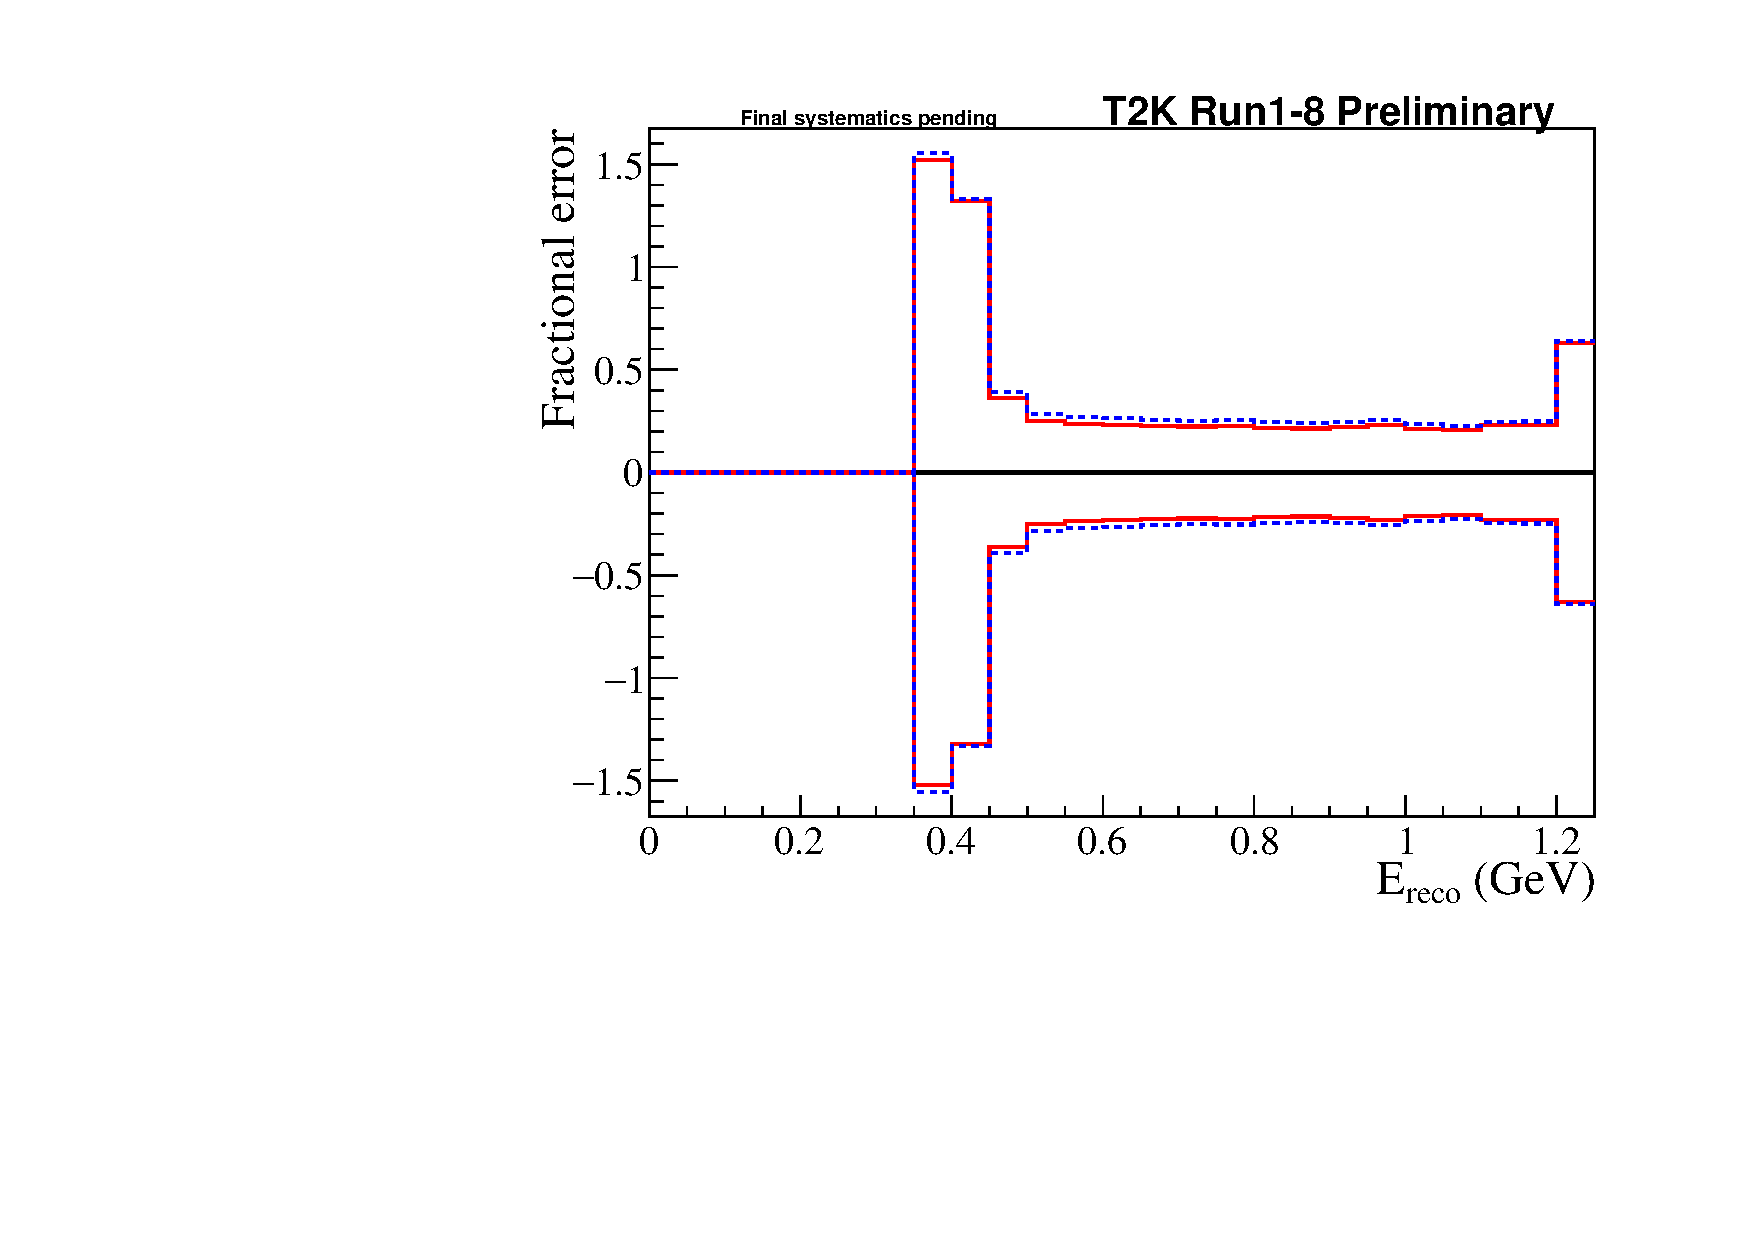
\includegraphics[width=0.9\textwidth]{systematics/envelopes/sk_errors/sk_error_table_MultiRe_all_envelope_fractional}
		\caption{\nueCConepi-like, neutrino mode}
	\end{subfigure}
	\caption {
		Error envelopes (left) and fractional errors (right) for the reconstructed neutrino energy spectrum for all systematic parameters for pre-BANFF (blue) and post-BANFF (red) errors. \num{1e4} toys are generated for the Asimov data set A with randomized systematic parameters with correlations taken into account. Since \deltacp, \ssqthtwothree, \dmsqtwothree and the mass hierarchy will be measured, only the uncertainty on \ssqthonethree, \ssqthonetwo and \dmsqonetwo are taken into account.
	}
	\label{fig:sk_envelopes_all}
\end{figure*}
\clearpage
\begin{figure*}
	\center
	\begin{subfigure}[b]{0.49\textwidth}
		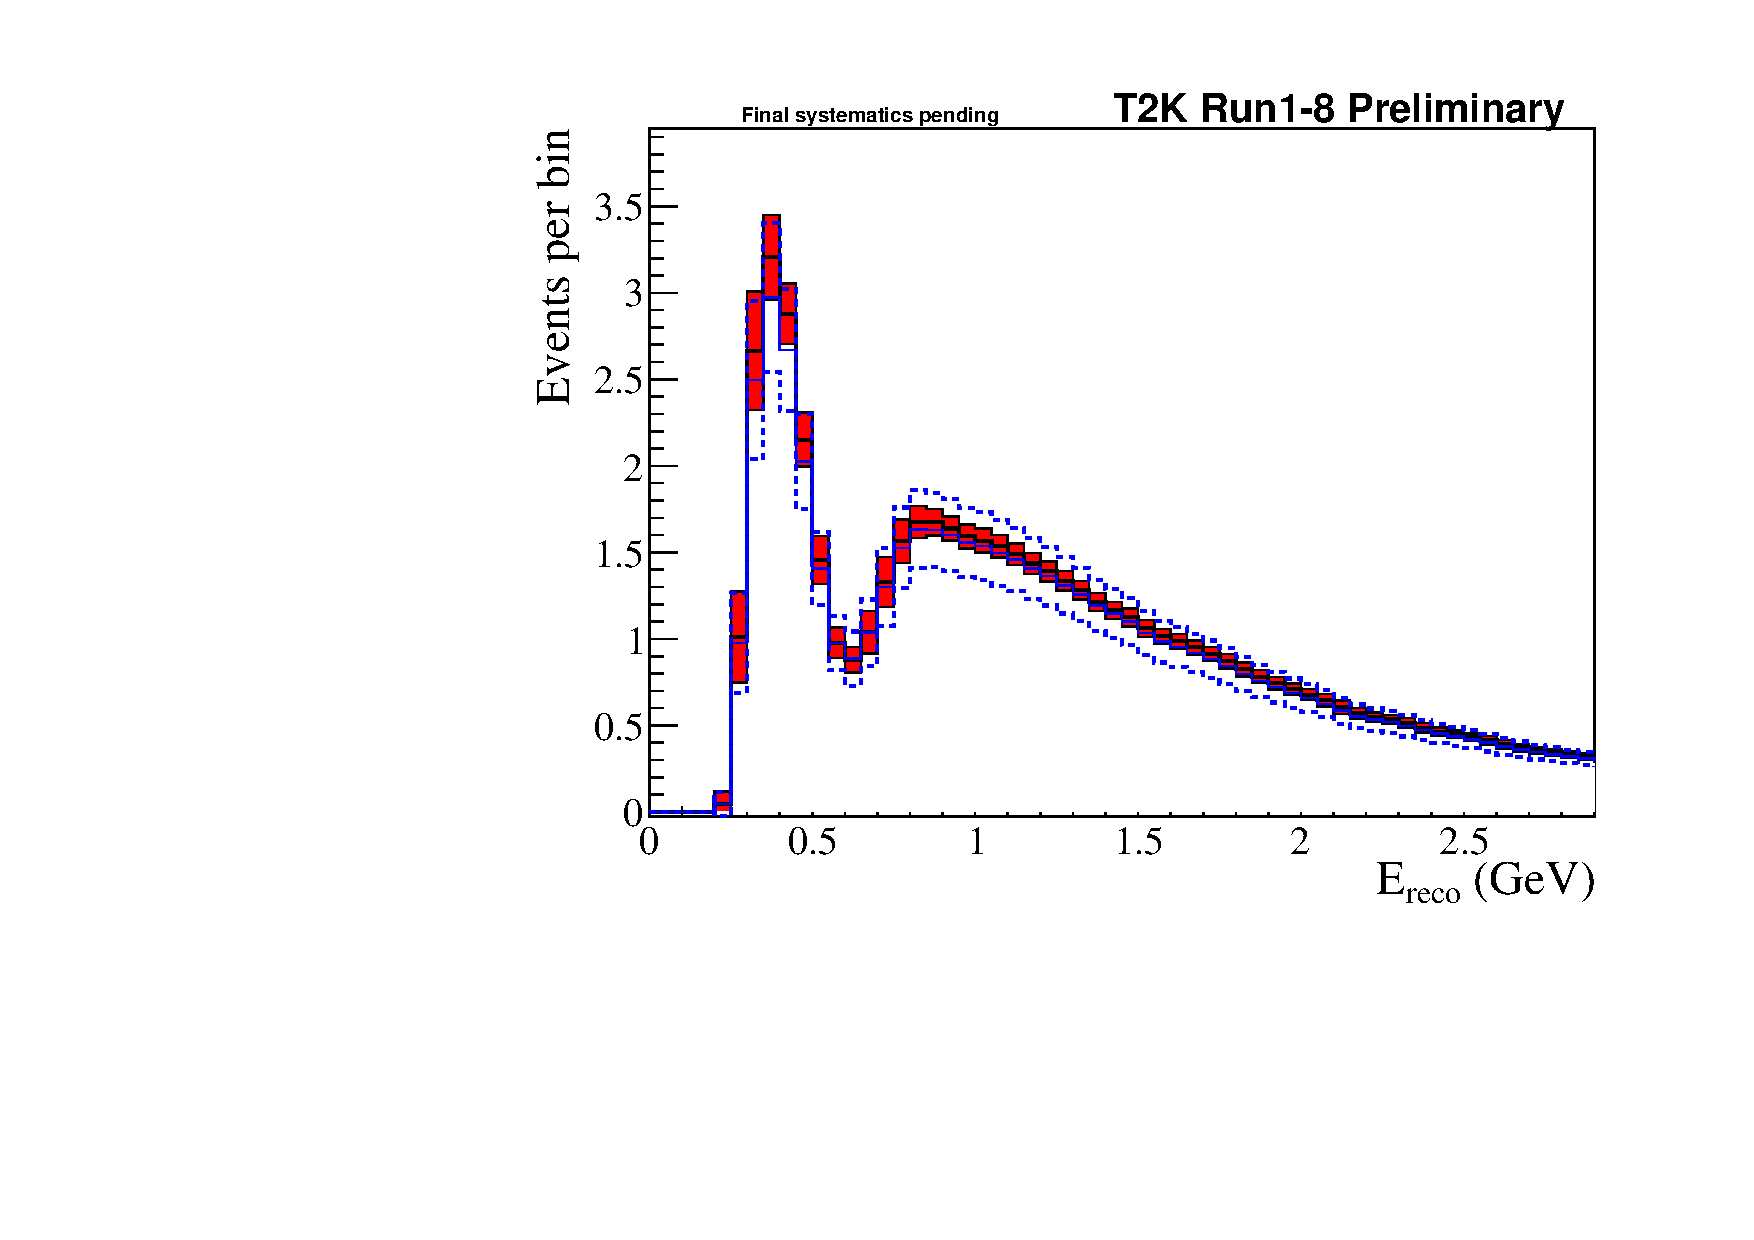
\includegraphics[width=0.9\textwidth]{systematics/envelopes/sk_errors/sk_error_table_RHC1Rmu_all_envelope}
		\caption{Muon-like, antineutrino mode}
	\end{subfigure}
	\begin{subfigure}[b]{0.49\textwidth}
		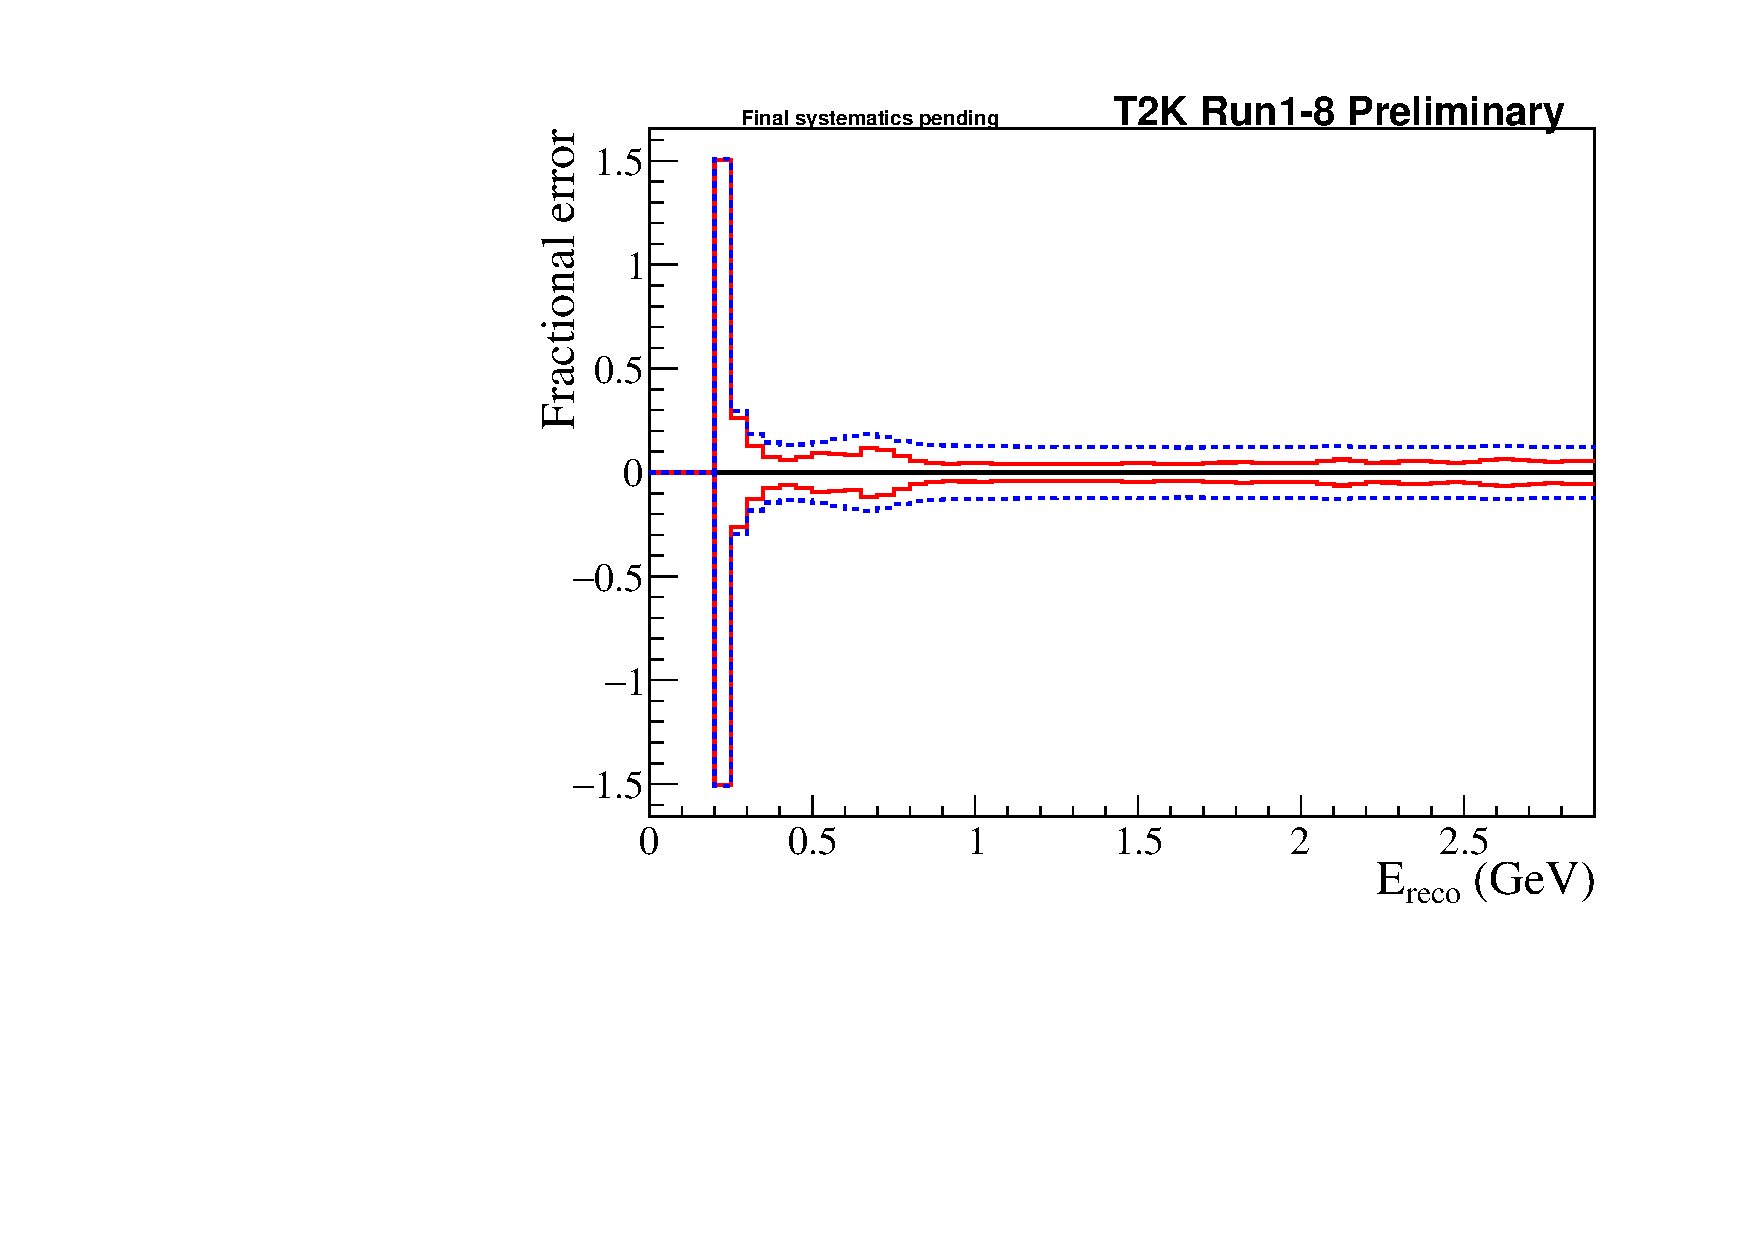
\includegraphics[width=0.9\textwidth]{systematics/envelopes/sk_errors/sk_error_table_RHC1Rmu_all_envelope_fractional}
		\caption{Muon-like, antineutrino mode}
	\end{subfigure}
	\begin{subfigure}[b]{0.49\textwidth}
		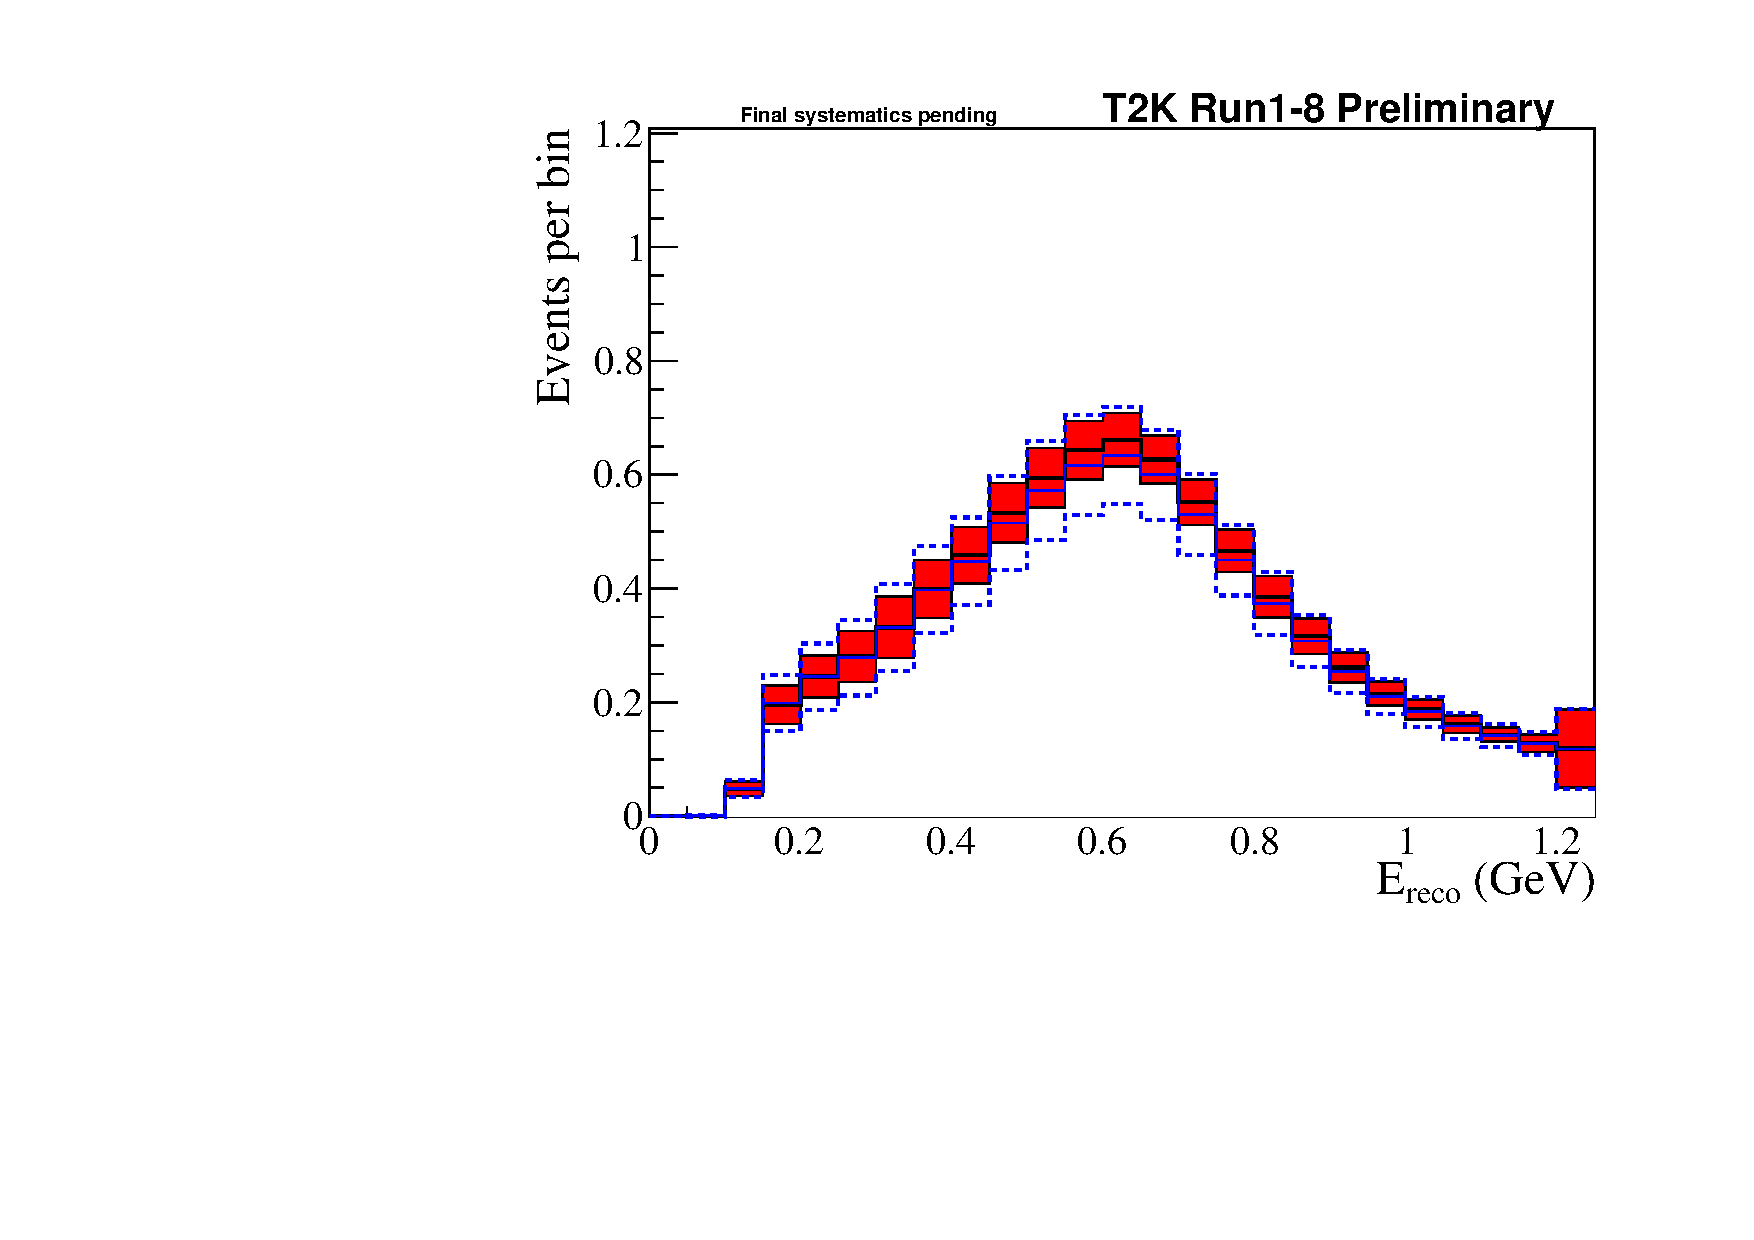
\includegraphics[width=0.9\textwidth]{systematics/envelopes/sk_errors/sk_error_table_RHC1Re_all_envelope}
		\caption{Electron-like antineutrino mode}
	\end{subfigure}
	\begin{subfigure}[b]{0.49\textwidth}
		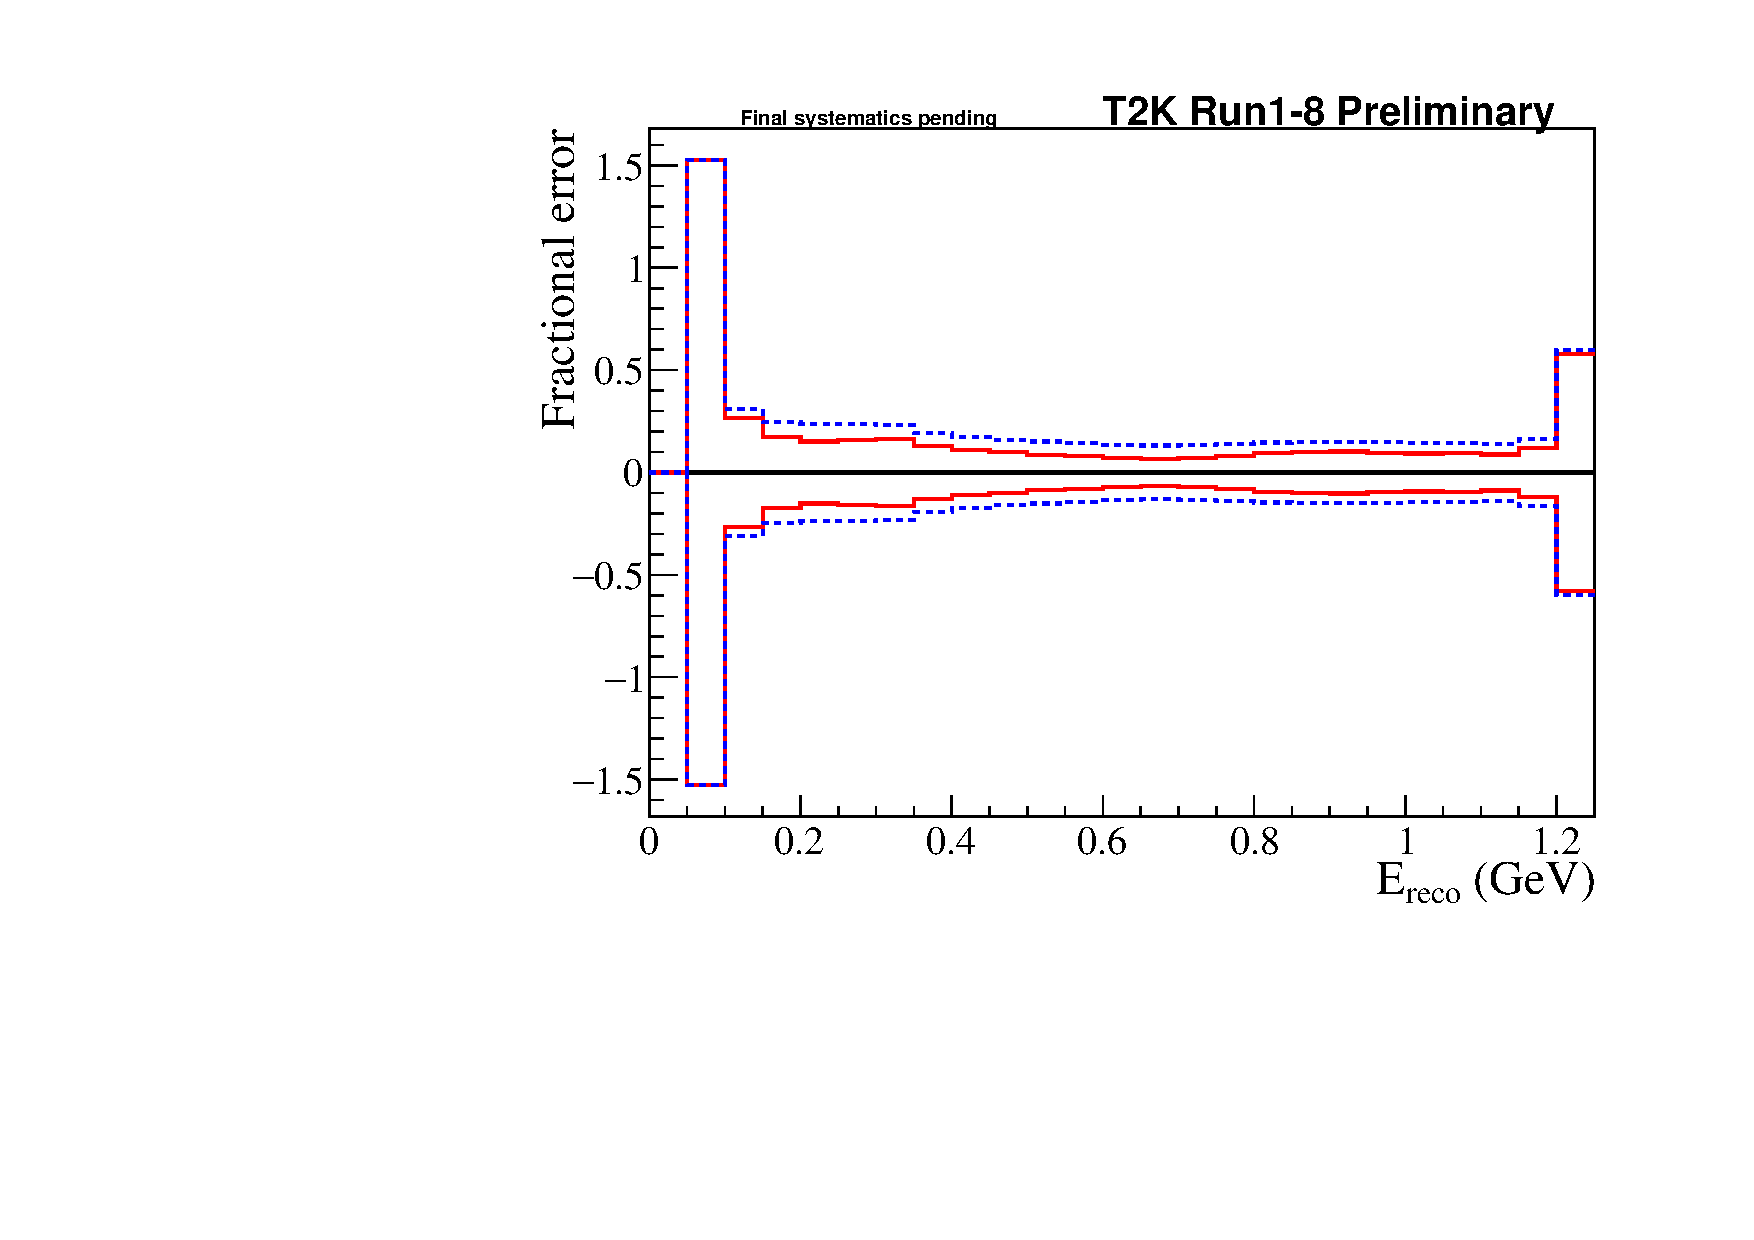
\includegraphics[width=0.9\textwidth]{systematics/envelopes/sk_errors/sk_error_table_RHC1Re_all_envelope_fractional}
		\caption{Electron-like antineutrino mode}
	\end{subfigure}
	\caption {
		Error envelopes (left) and fractional errors (right) for the reconstructed neutrino energy spectrum for all systematic parameters for pre-BANFF (blue) and post-BANFF (red) errors. \num{1e4} toys are generated for the Asimov data set A with randomized systematic parameters with correlations taken into account. Since \deltacp, \ssqthtwothree, \dmsqtwothree and the mass hierarchy will be measured, only the uncertainty on \ssqthonethree, \ssqthonetwo and \dmsqonetwo are taken into account.
	}
	\label{fig:sk_envelopes_all_b}
\end{figure*}
\clearpage
\begin{figure*}
	\center
	\begin{subfigure}[b]{0.49\textwidth}
		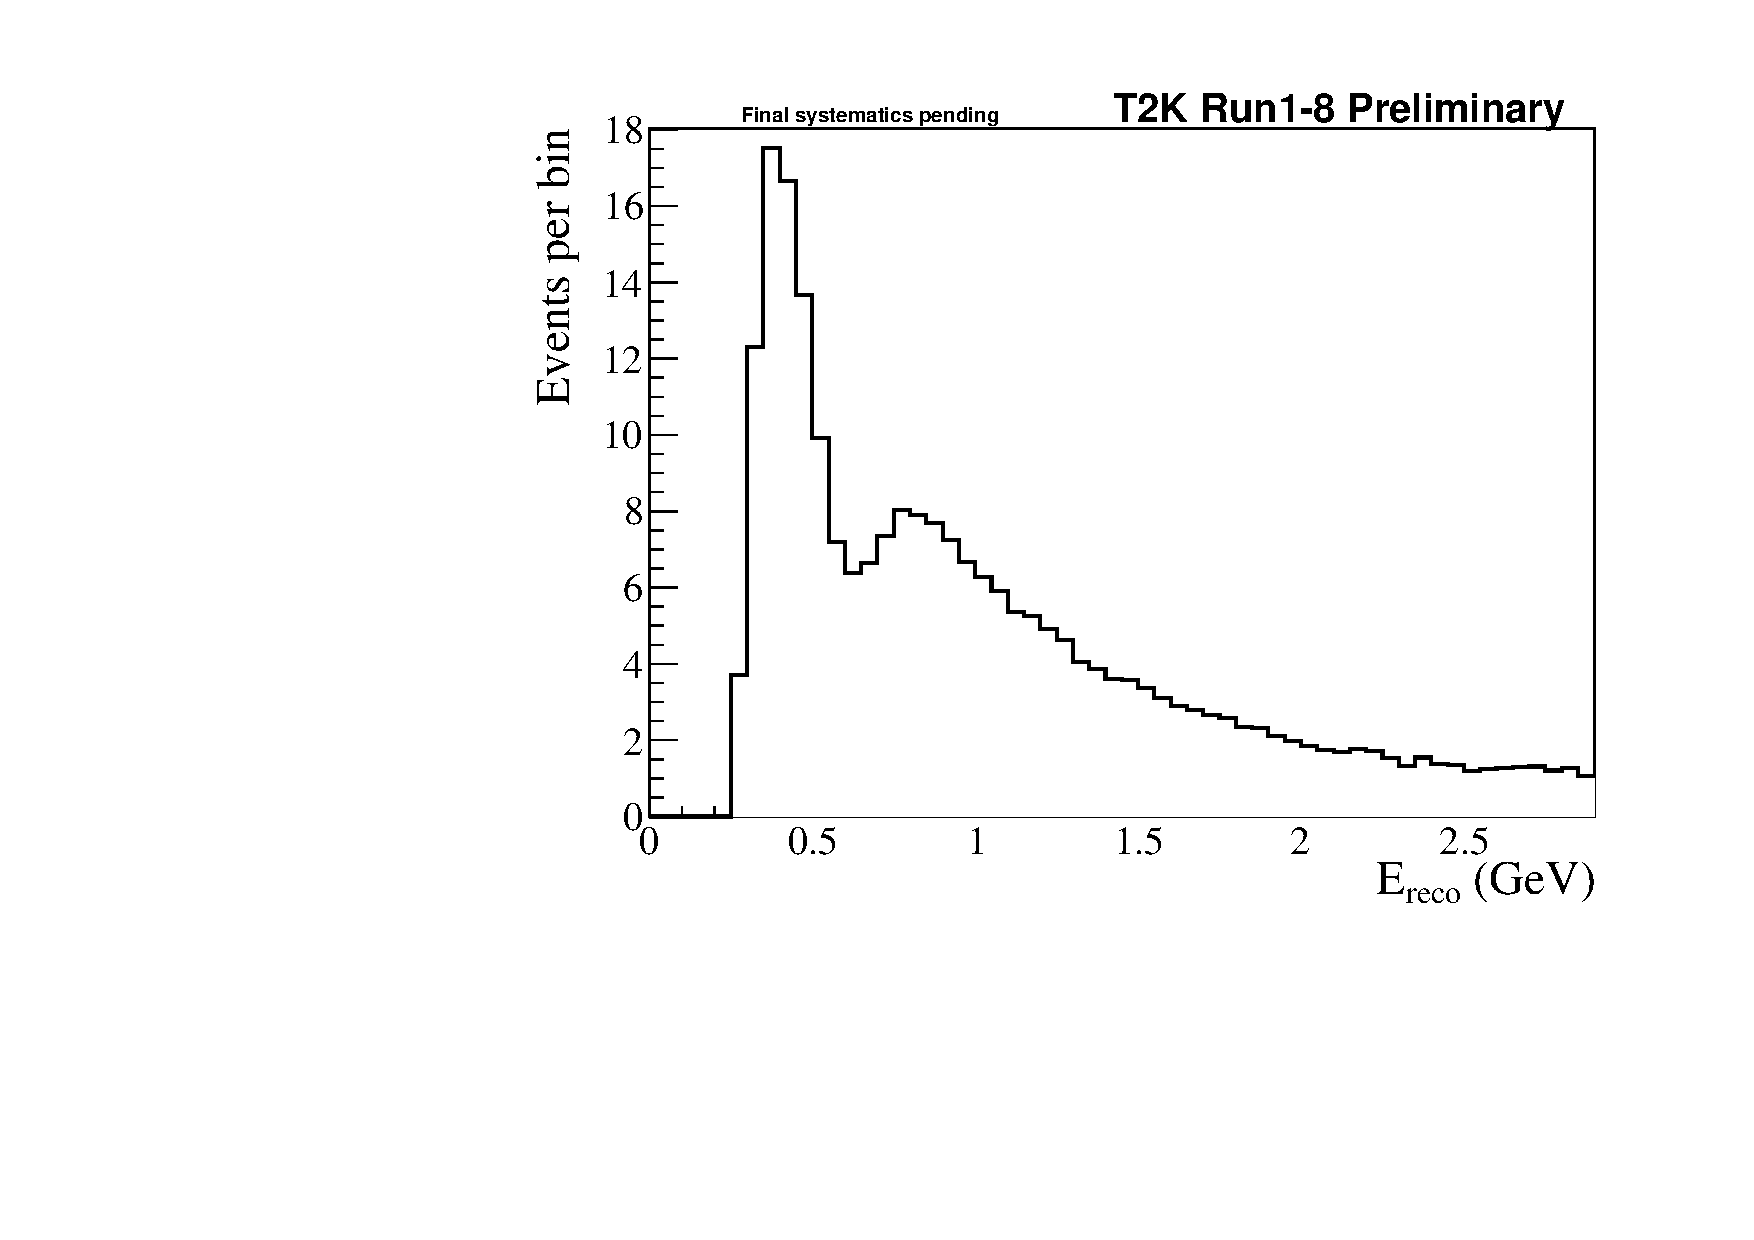
\includegraphics[width=0.9\textwidth]{systematics/envelopes/sk_errors/sk_error_table_1Rmu_osc_envelope}
		\caption{Muon-like, neutrino mode}
	\end{subfigure}
	\begin{subfigure}[b]{0.49\textwidth}
		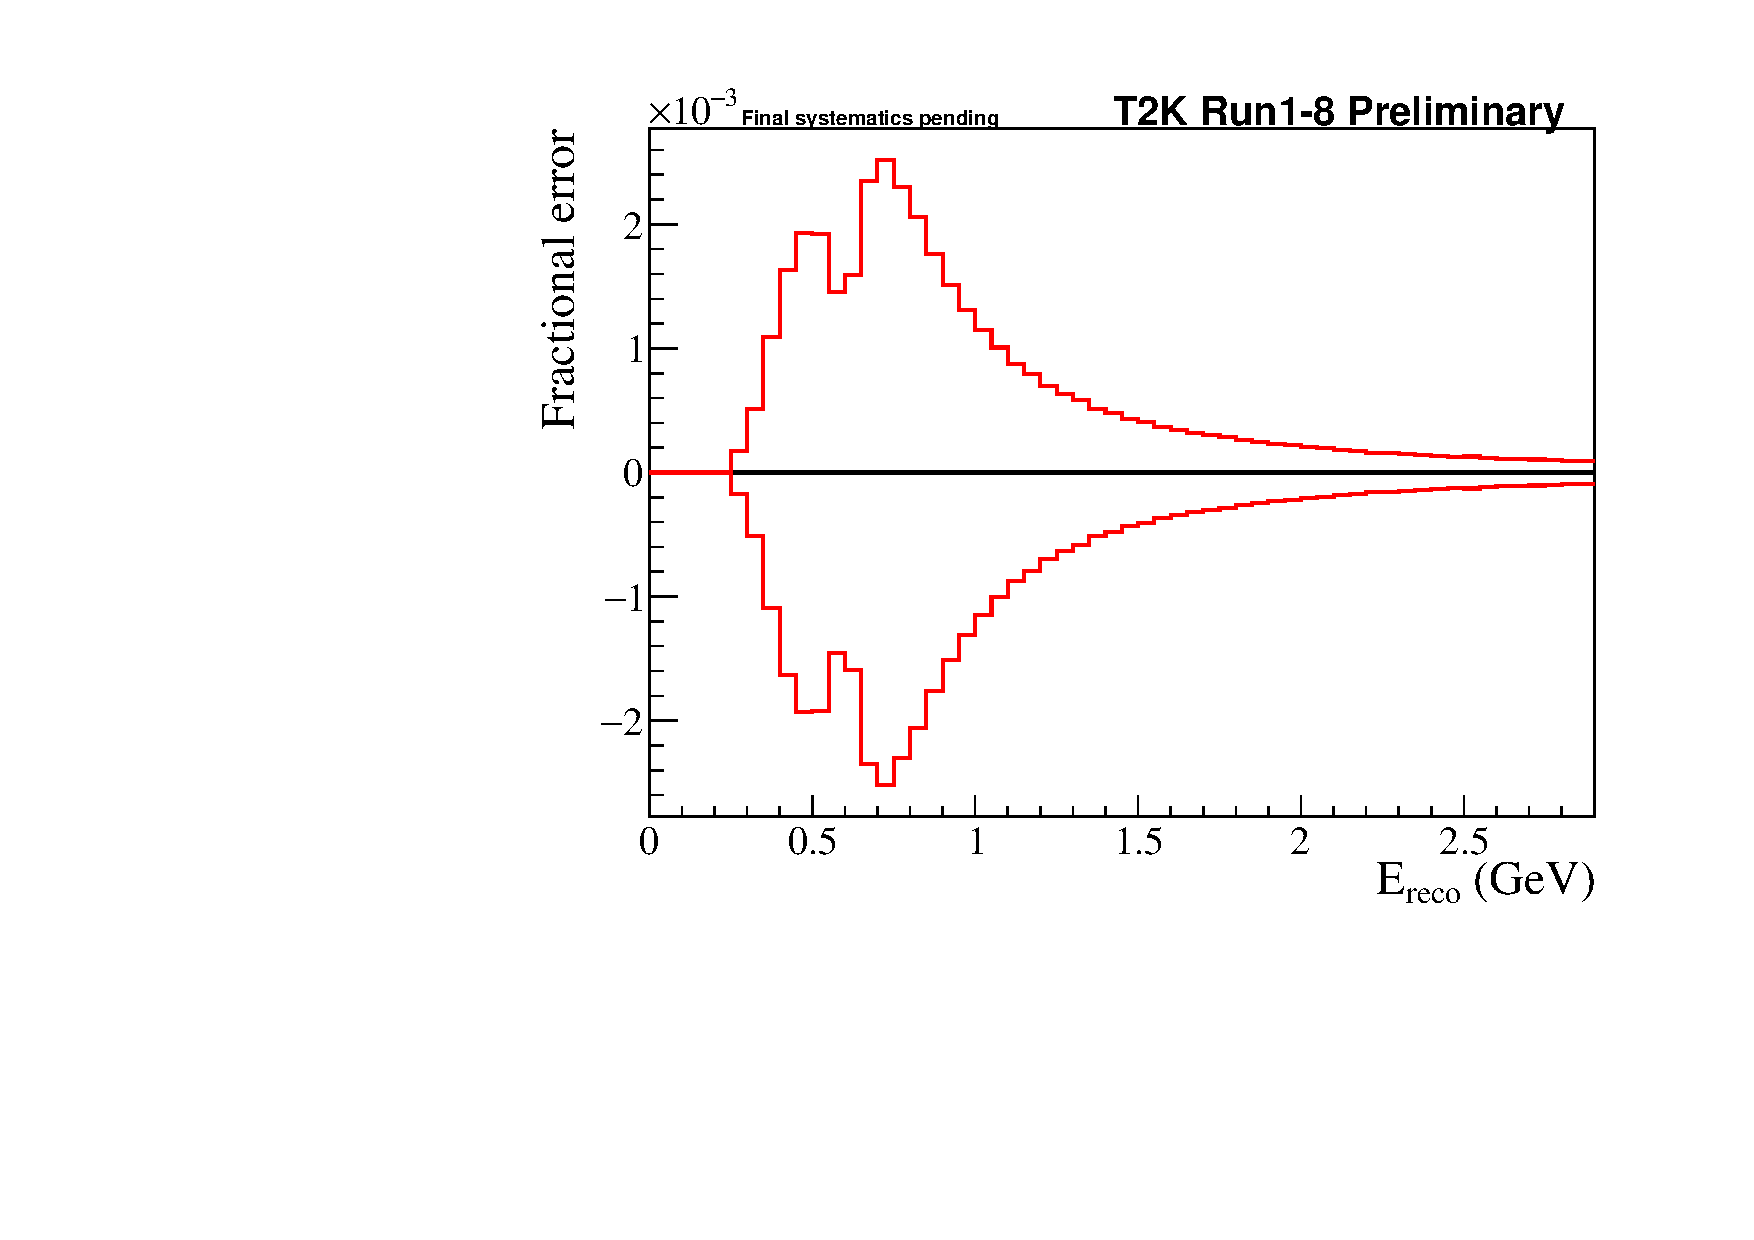
\includegraphics[width=0.9\textwidth]{systematics/envelopes/sk_errors/sk_error_table_1Rmu_osc_envelope_fractional}
		\caption{Muon-like, neutrino mode}
	\end{subfigure}
	\begin{subfigure}[b]{0.49\textwidth}
		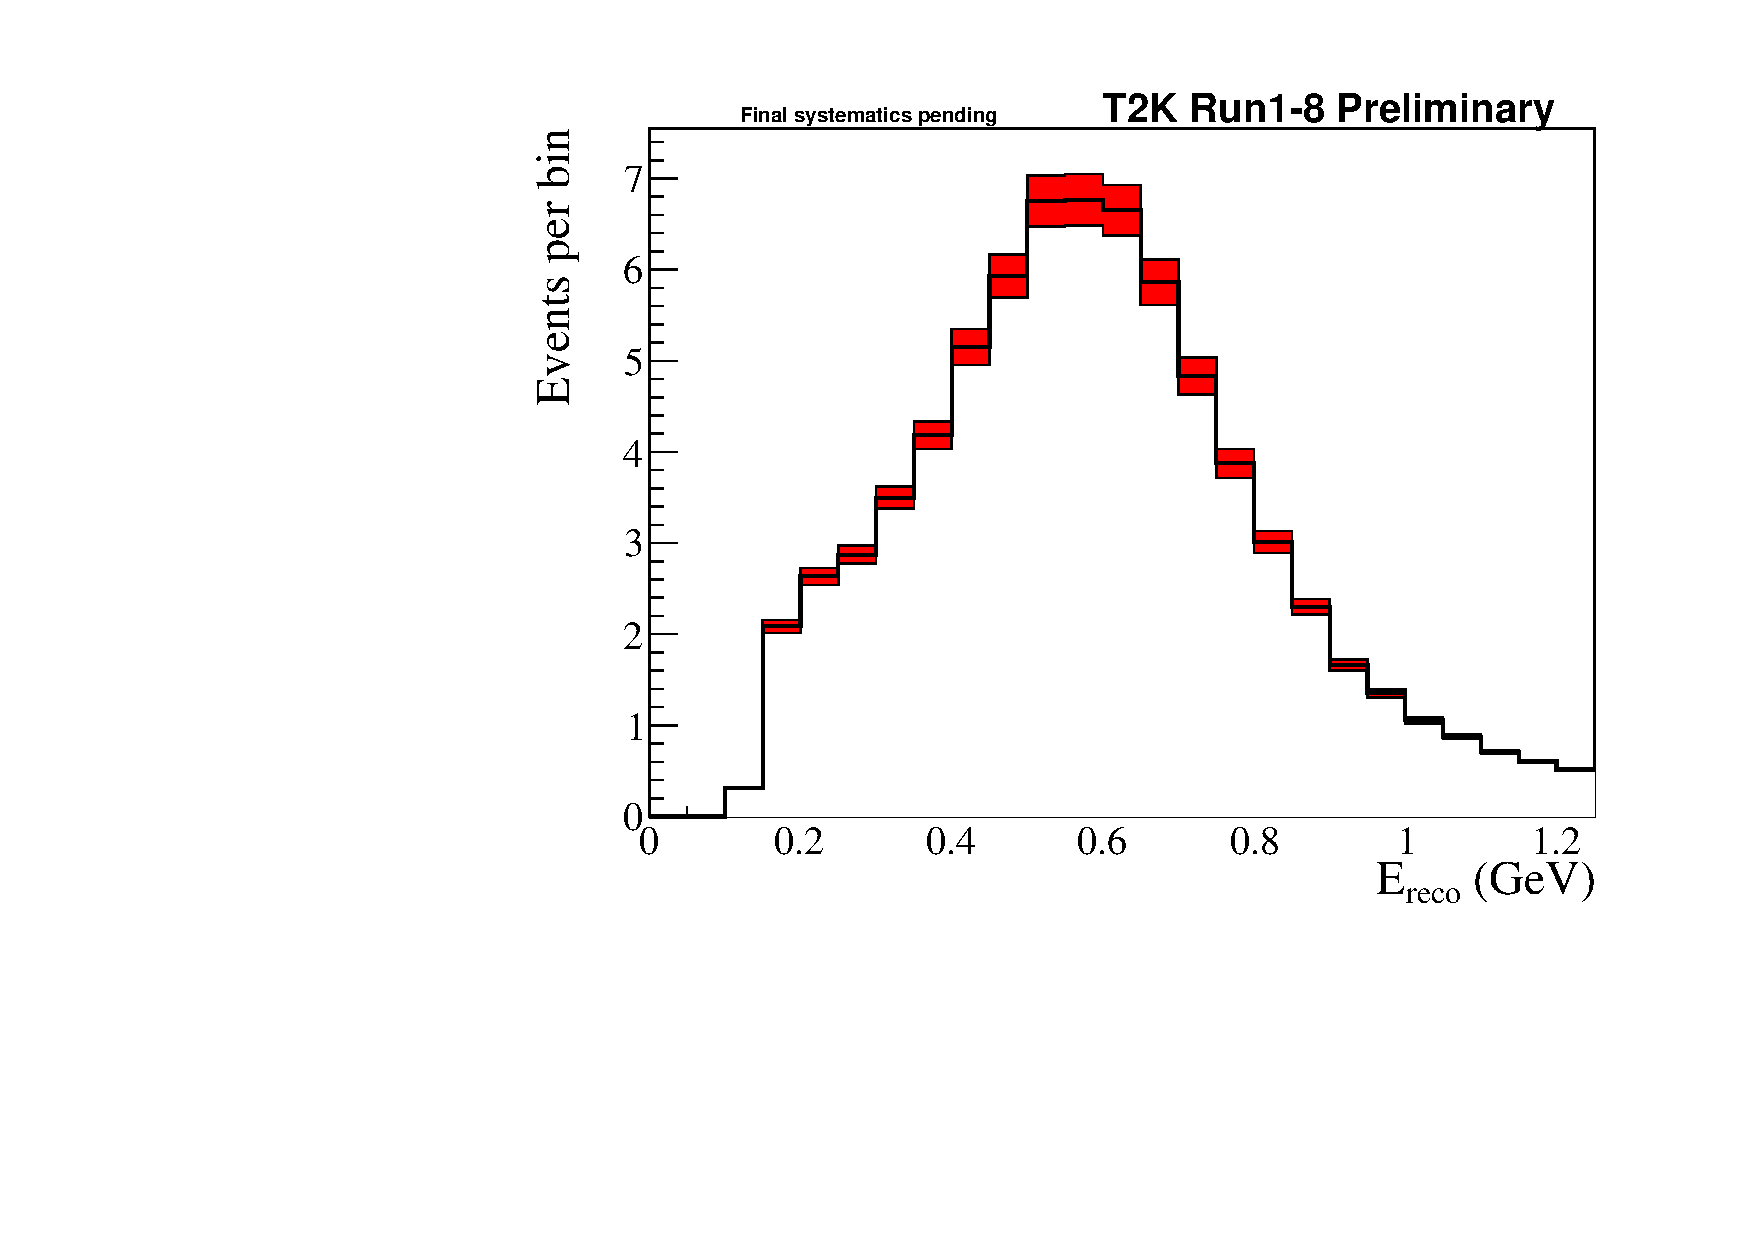
\includegraphics[width=0.9\textwidth]{systematics/envelopes/sk_errors/sk_error_table_1Re_osc_envelope}
		\caption{Electron-like, neutrino mode}
	\end{subfigure}
	\begin{subfigure}[b]{0.49\textwidth}
		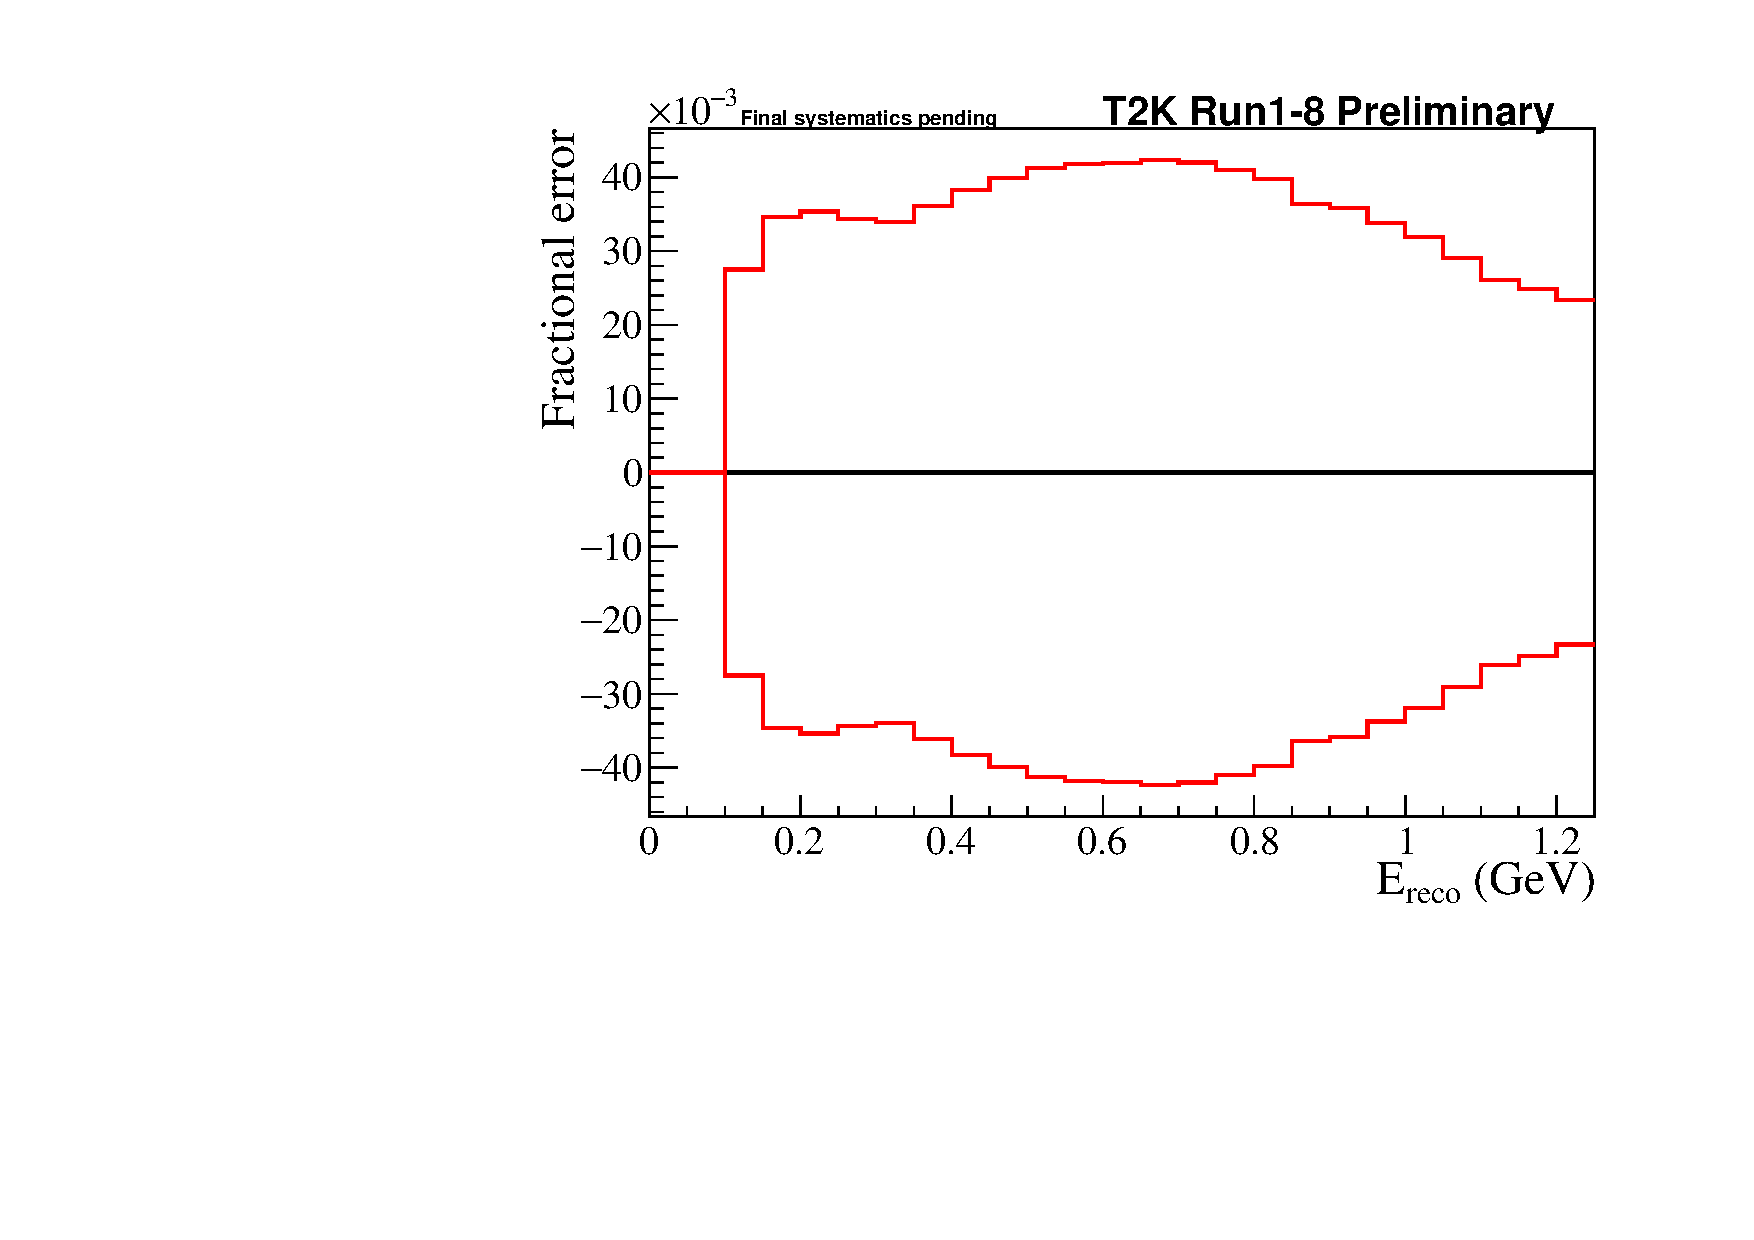
\includegraphics[width=0.9\textwidth]{systematics/envelopes/sk_errors/sk_error_table_1Re_osc_envelope_fractional}
		\caption{Electron-like, neutrino mode}
	\end{subfigure}
	\begin{subfigure}[b]{0.49\textwidth}
		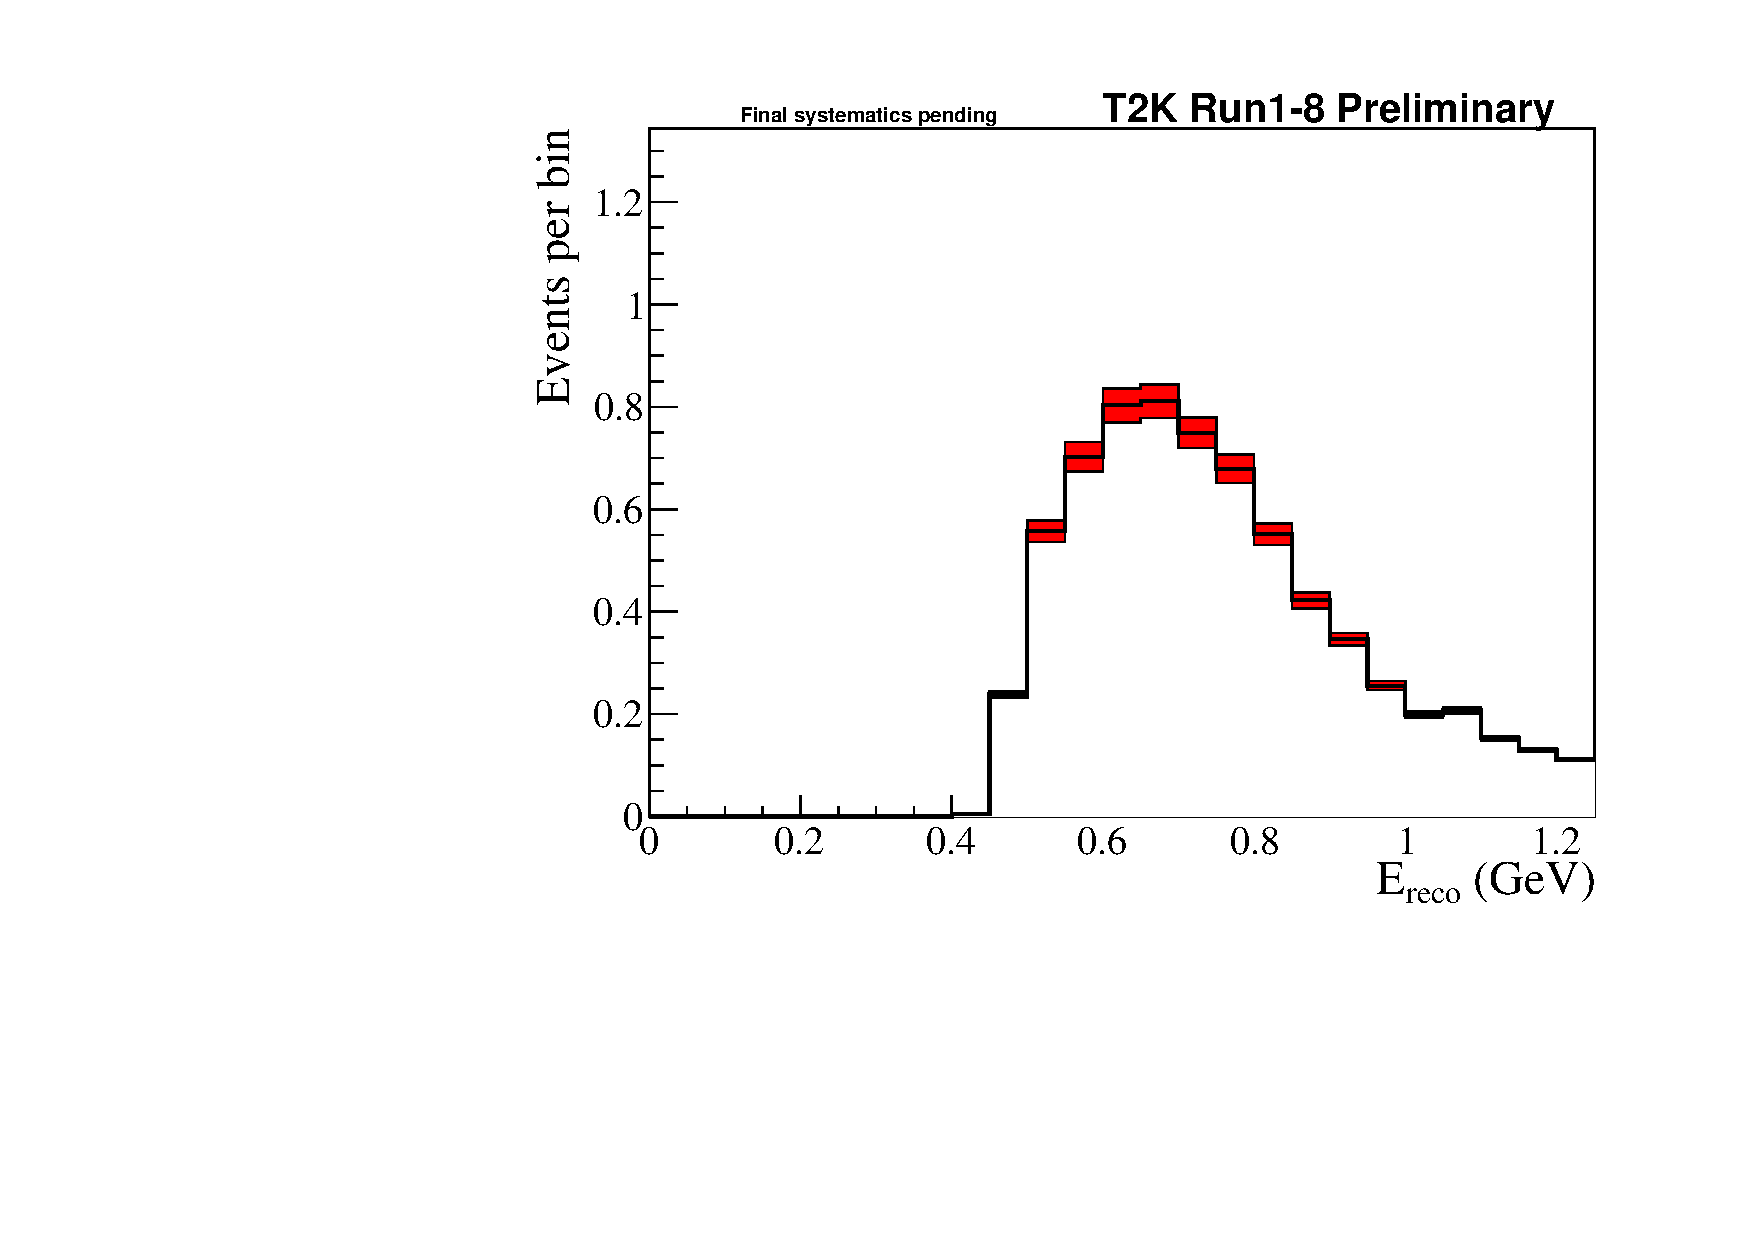
\includegraphics[width=0.9\textwidth]{systematics/envelopes/sk_errors/sk_error_table_MultiRe_osc_envelope}
		\caption{\nueCConepi-like, neutrino mode}
	\end{subfigure}
	\begin{subfigure}[b]{0.49\textwidth}
		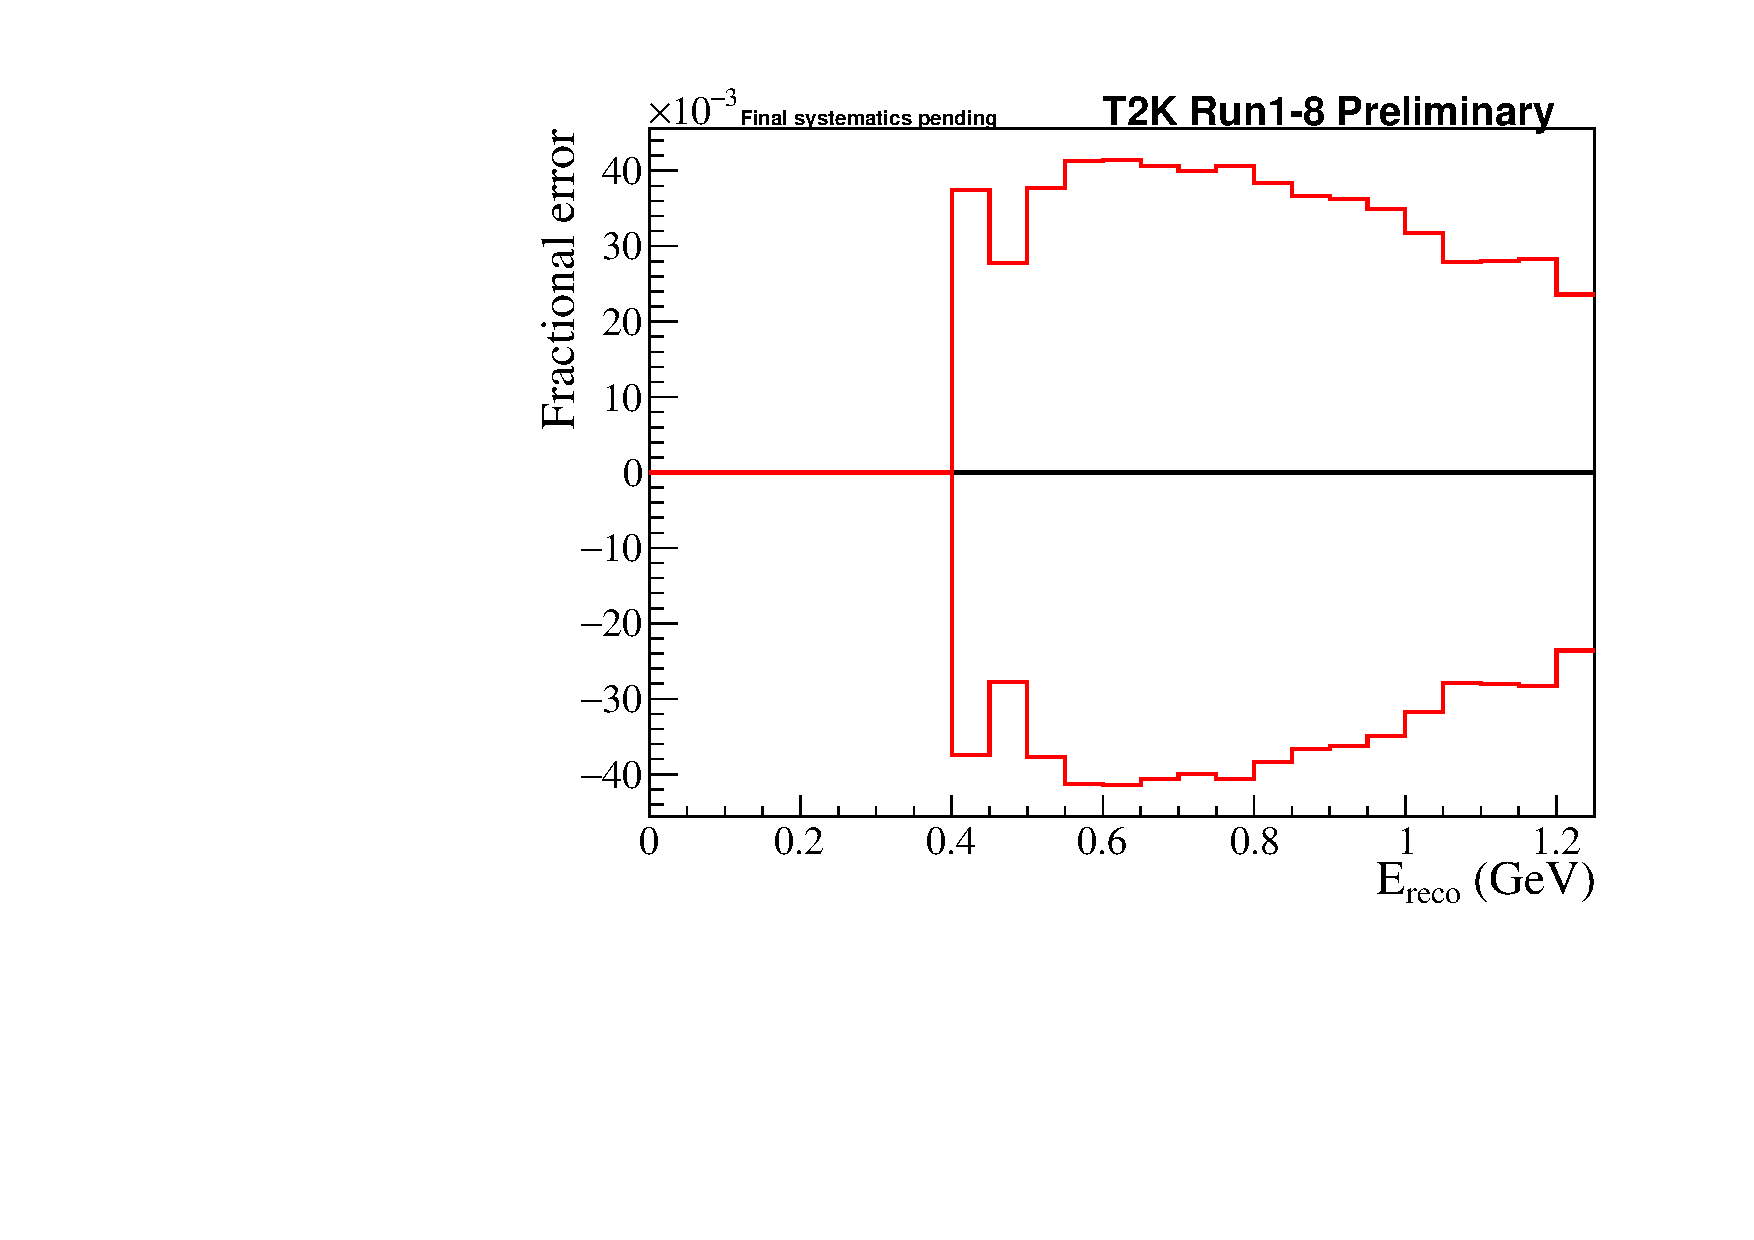
\includegraphics[width=0.9\textwidth]{systematics/envelopes/sk_errors/sk_error_table_MultiRe_osc_envelope_fractional}
		\caption{\nueCConepi-like, neutrino mode}
	\end{subfigure}
	\caption {
		Error envelopes (left) and fractional errors (right) for the reconstructed neutrino energy spectrum for all oscillation nuisance parameters. \num{1e4} toys are generated for the Asimov data set A with randomized systematic parameters with correlations taken into account. Since \deltacp, \ssqthtwothree, \dmsqtwothree and the mass hierarchy will be measured, only the uncertainty on \ssqthonethree, \ssqthonetwo and \dmsqonetwo are taken into account.
	}
	\label{fig:sk_envelopes_osc}
\end{figure*}
\clearpage

\begin{figure*}
	\center
	\begin{subfigure}[b]{0.49\textwidth}
		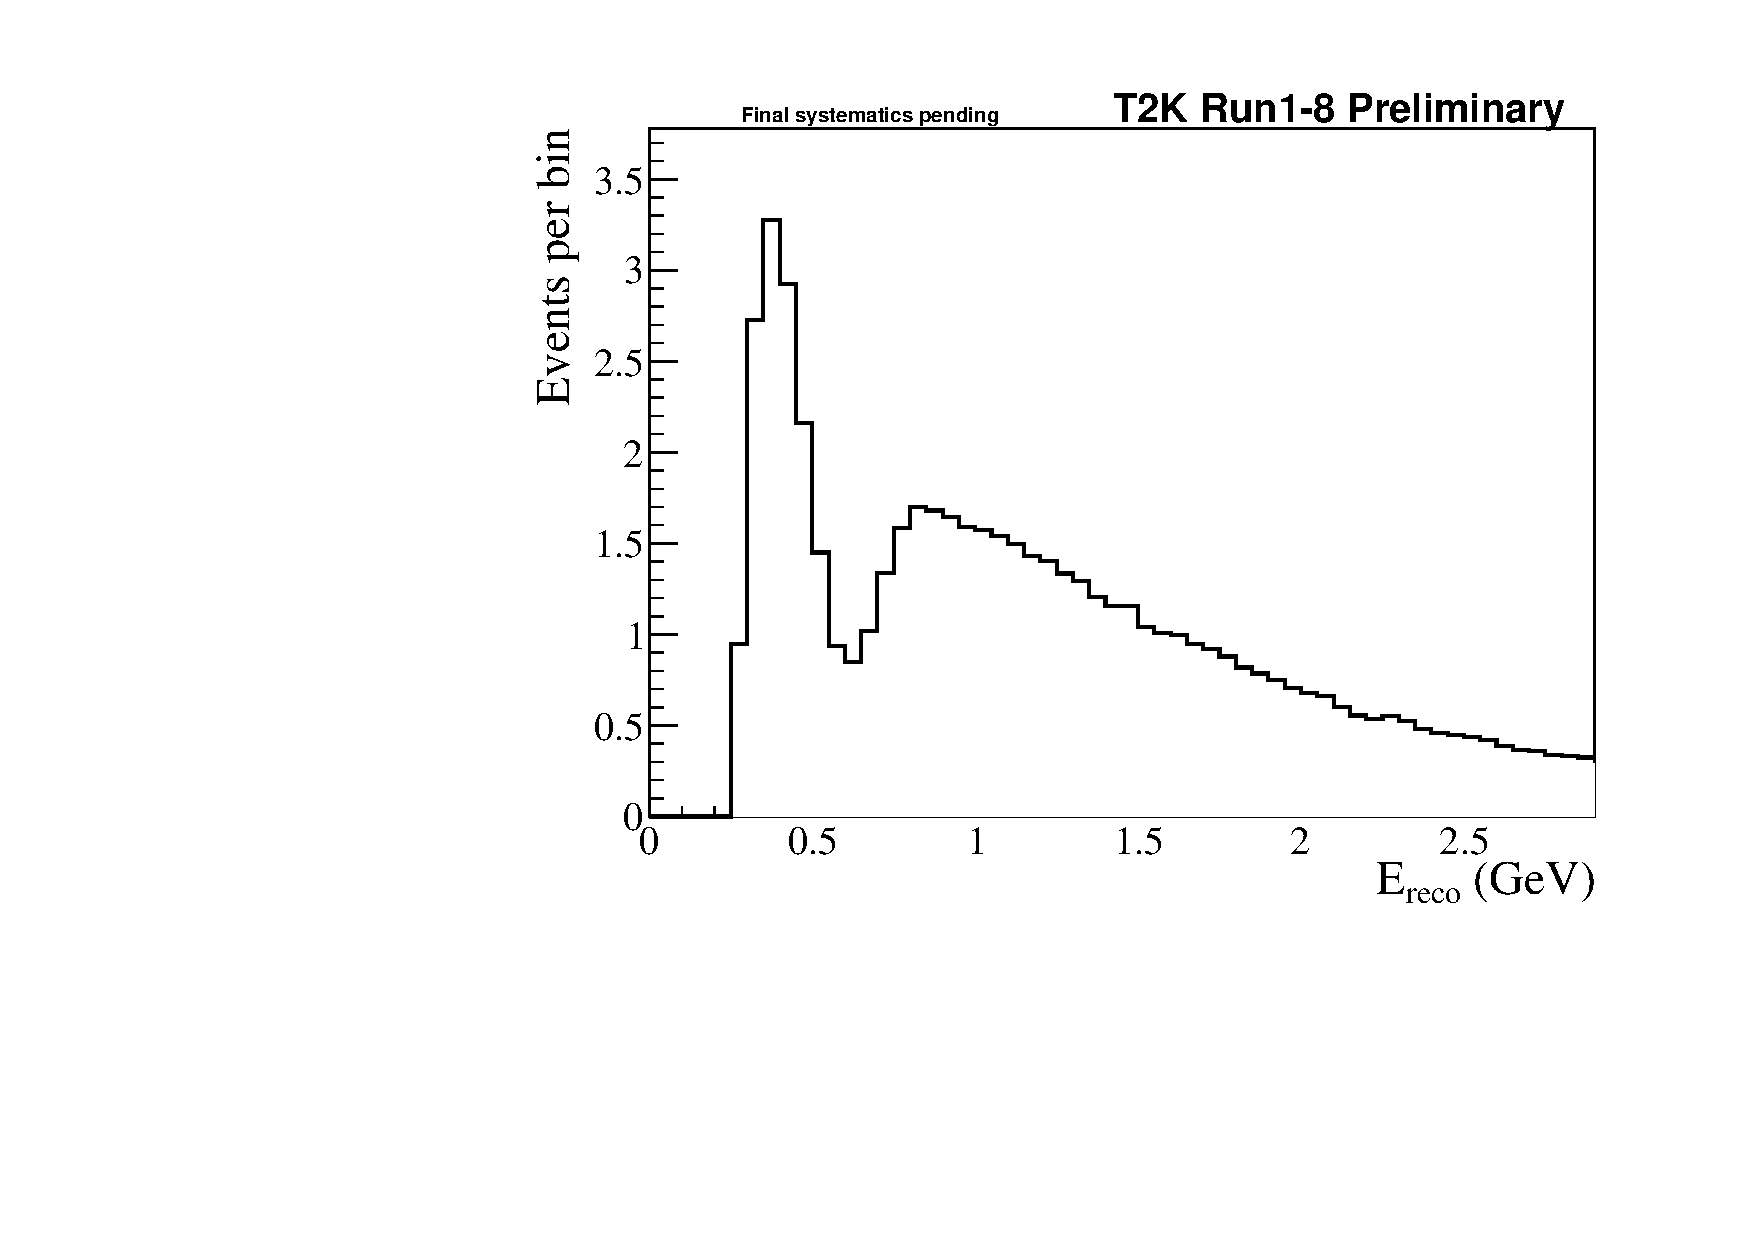
\includegraphics[width=0.9\textwidth]{systematics/envelopes/sk_errors/sk_error_table_RHC1Rmu_osc_envelope}
		\caption{Muon-like, antineutrino mode}
	\end{subfigure}
	\begin{subfigure}[b]{0.49\textwidth}
		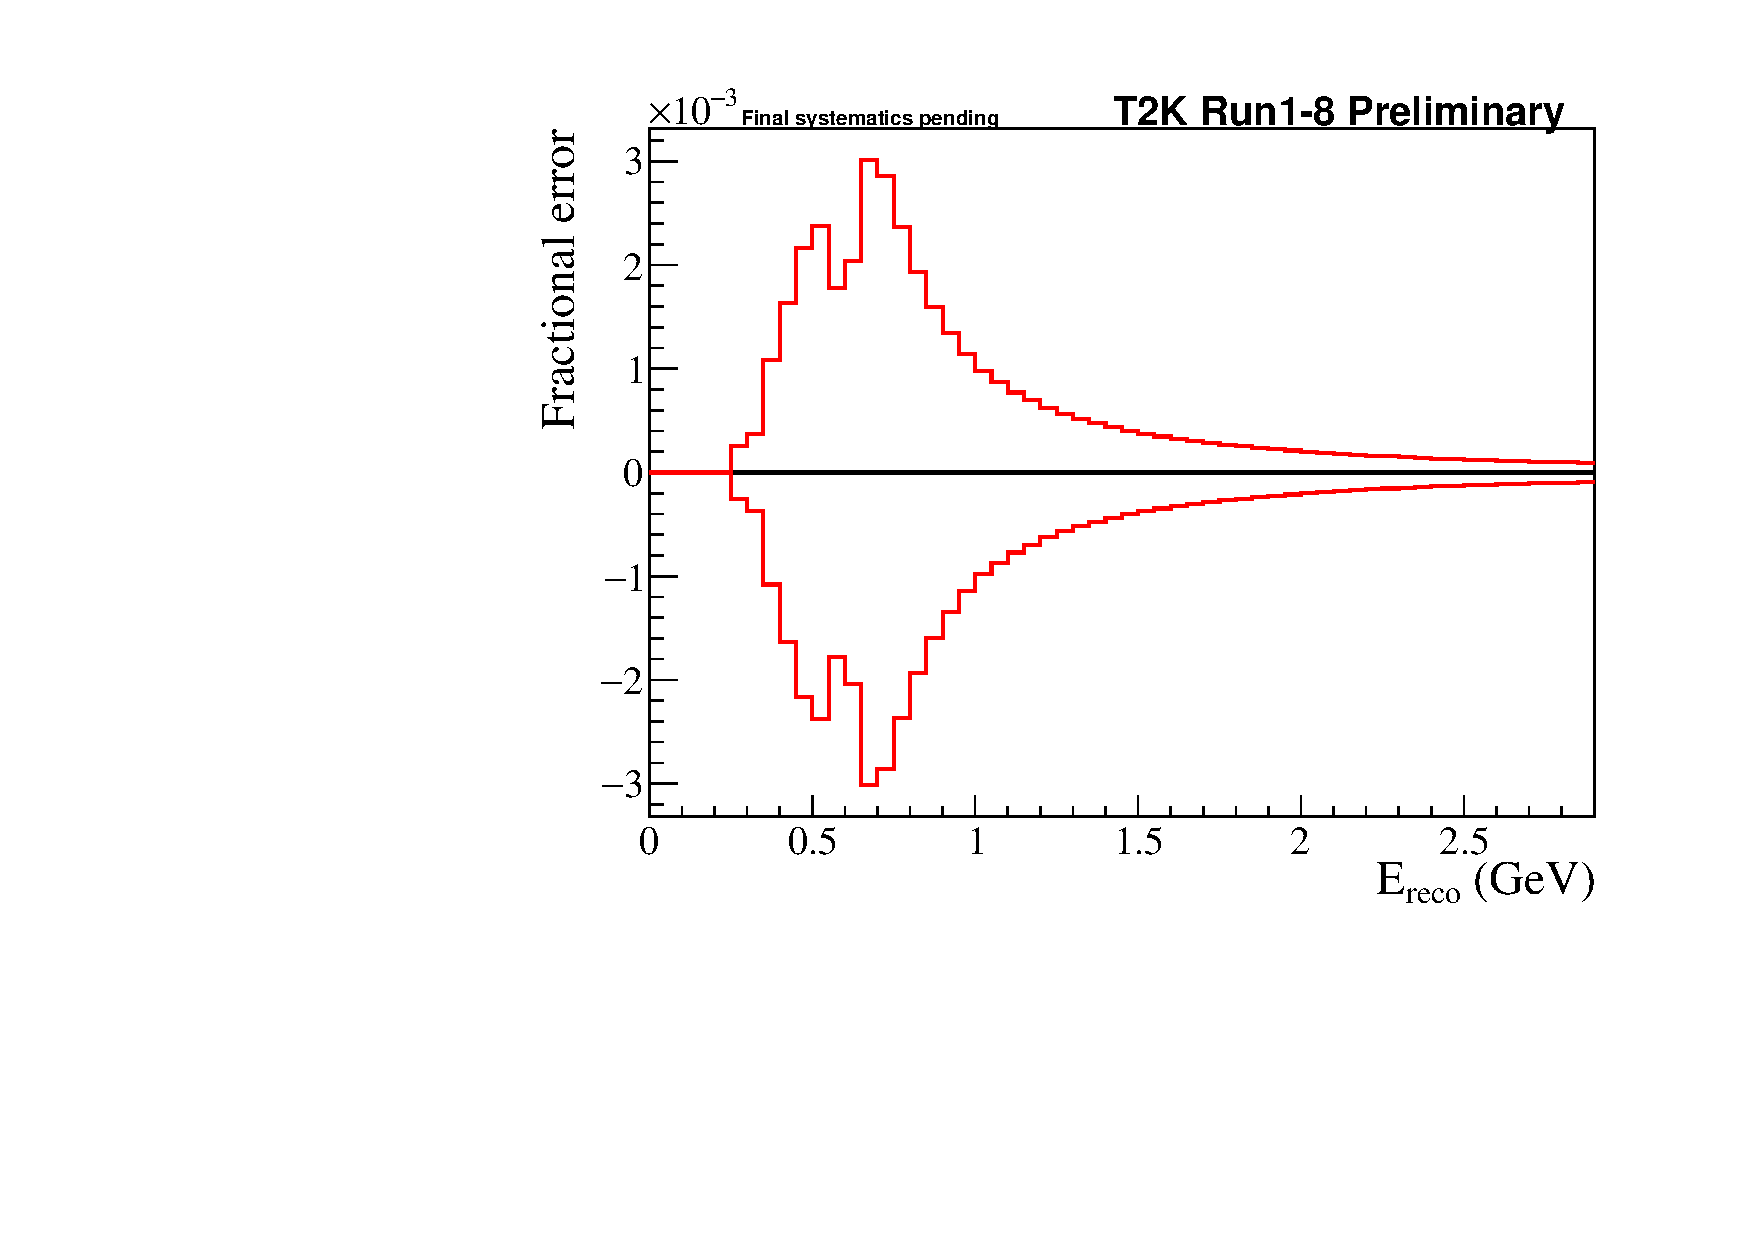
\includegraphics[width=0.9\textwidth]{systematics/envelopes/sk_errors/sk_error_table_RHC1Rmu_osc_envelope_fractional}
		\caption{Muon-like, antineutrino mode}
	\end{subfigure}
	\begin{subfigure}[b]{0.49\textwidth}
		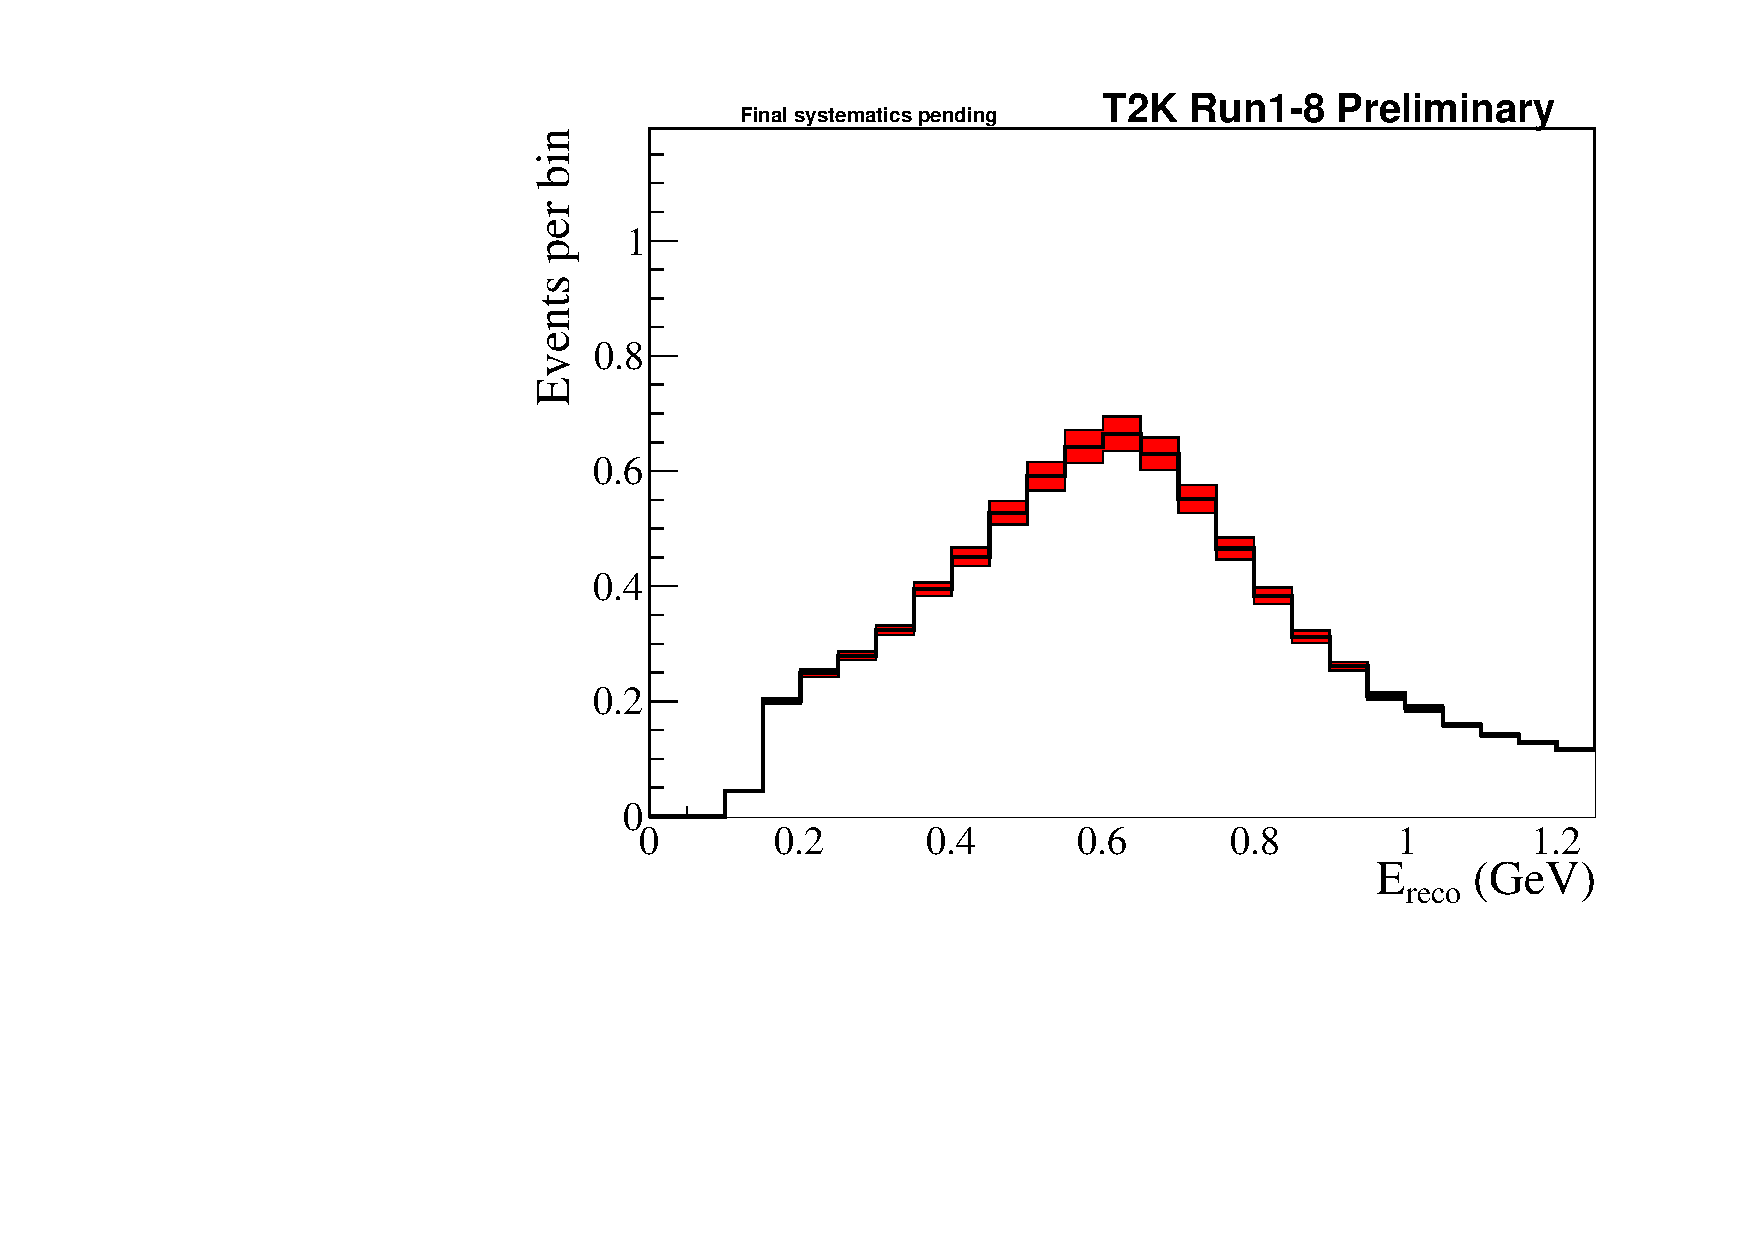
\includegraphics[width=0.9\textwidth]{systematics/envelopes/sk_errors/sk_error_table_RHC1Re_osc_envelope}
		\caption{Electron-like antineutrino mode}
	\end{subfigure}
	\begin{subfigure}[b]{0.49\textwidth}
		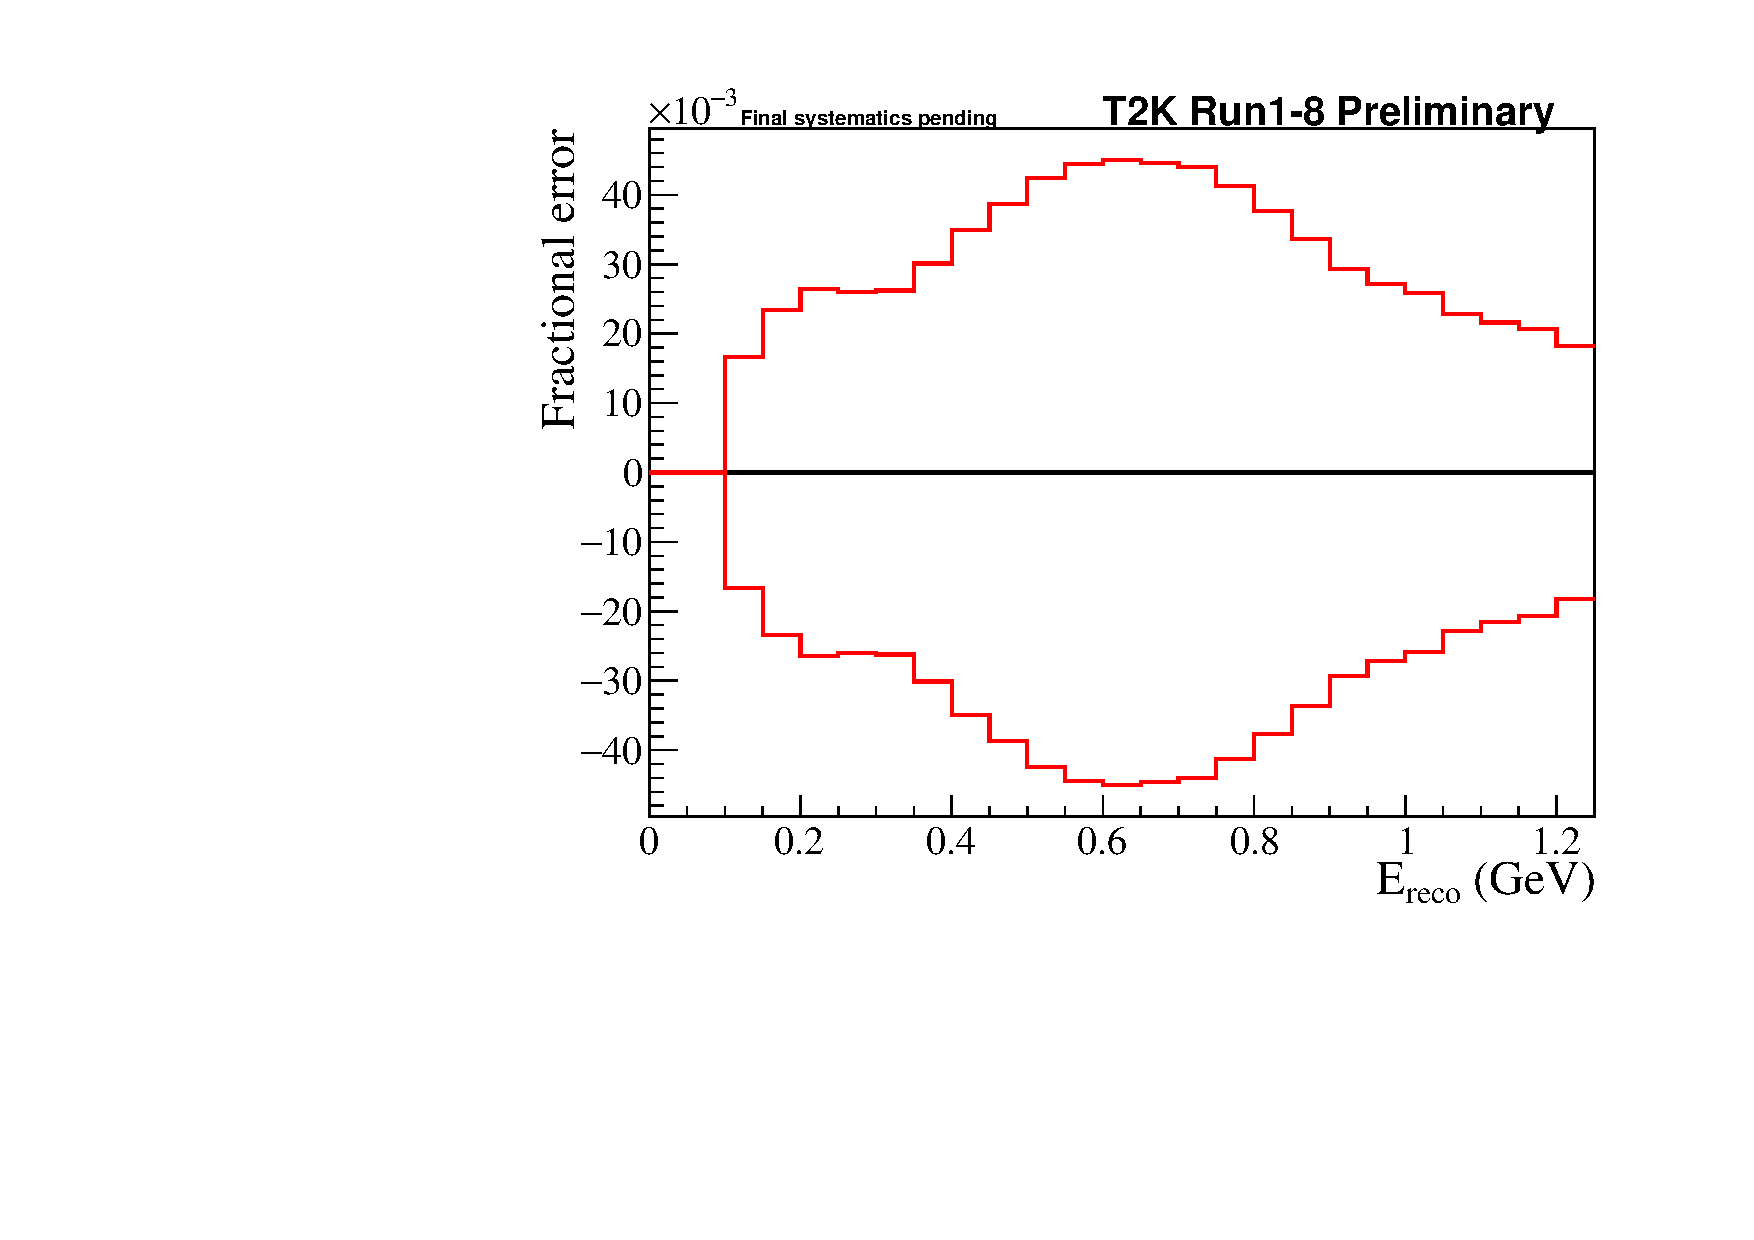
\includegraphics[width=0.9\textwidth]{systematics/envelopes/sk_errors/sk_error_table_RHC1Re_osc_envelope_fractional}
		\caption{Electron-like antineutrino mode}
	\end{subfigure}
	\caption {
		Error envelopes (left) and fractional errors (right) for the reconstructed neutrino energy spectrum for all oscillation nuisance parameters. \num{1e4} toys are generated for the Asimov data set A with randomized systematic parameters with correlations taken into account. Since \deltacp, \ssqthtwothree, \dmsqtwothree and the mass hierarchy will be measured, only the uncertainty on \ssqthonethree, \ssqthonetwo and \dmsqonetwo are taken into account.
	}
	\label{fig:sk_envelopes_osc_b}
\end{figure*}
\clearpage
\begin{figure*}
	\center
	\begin{subfigure}[b]{0.49\textwidth}
		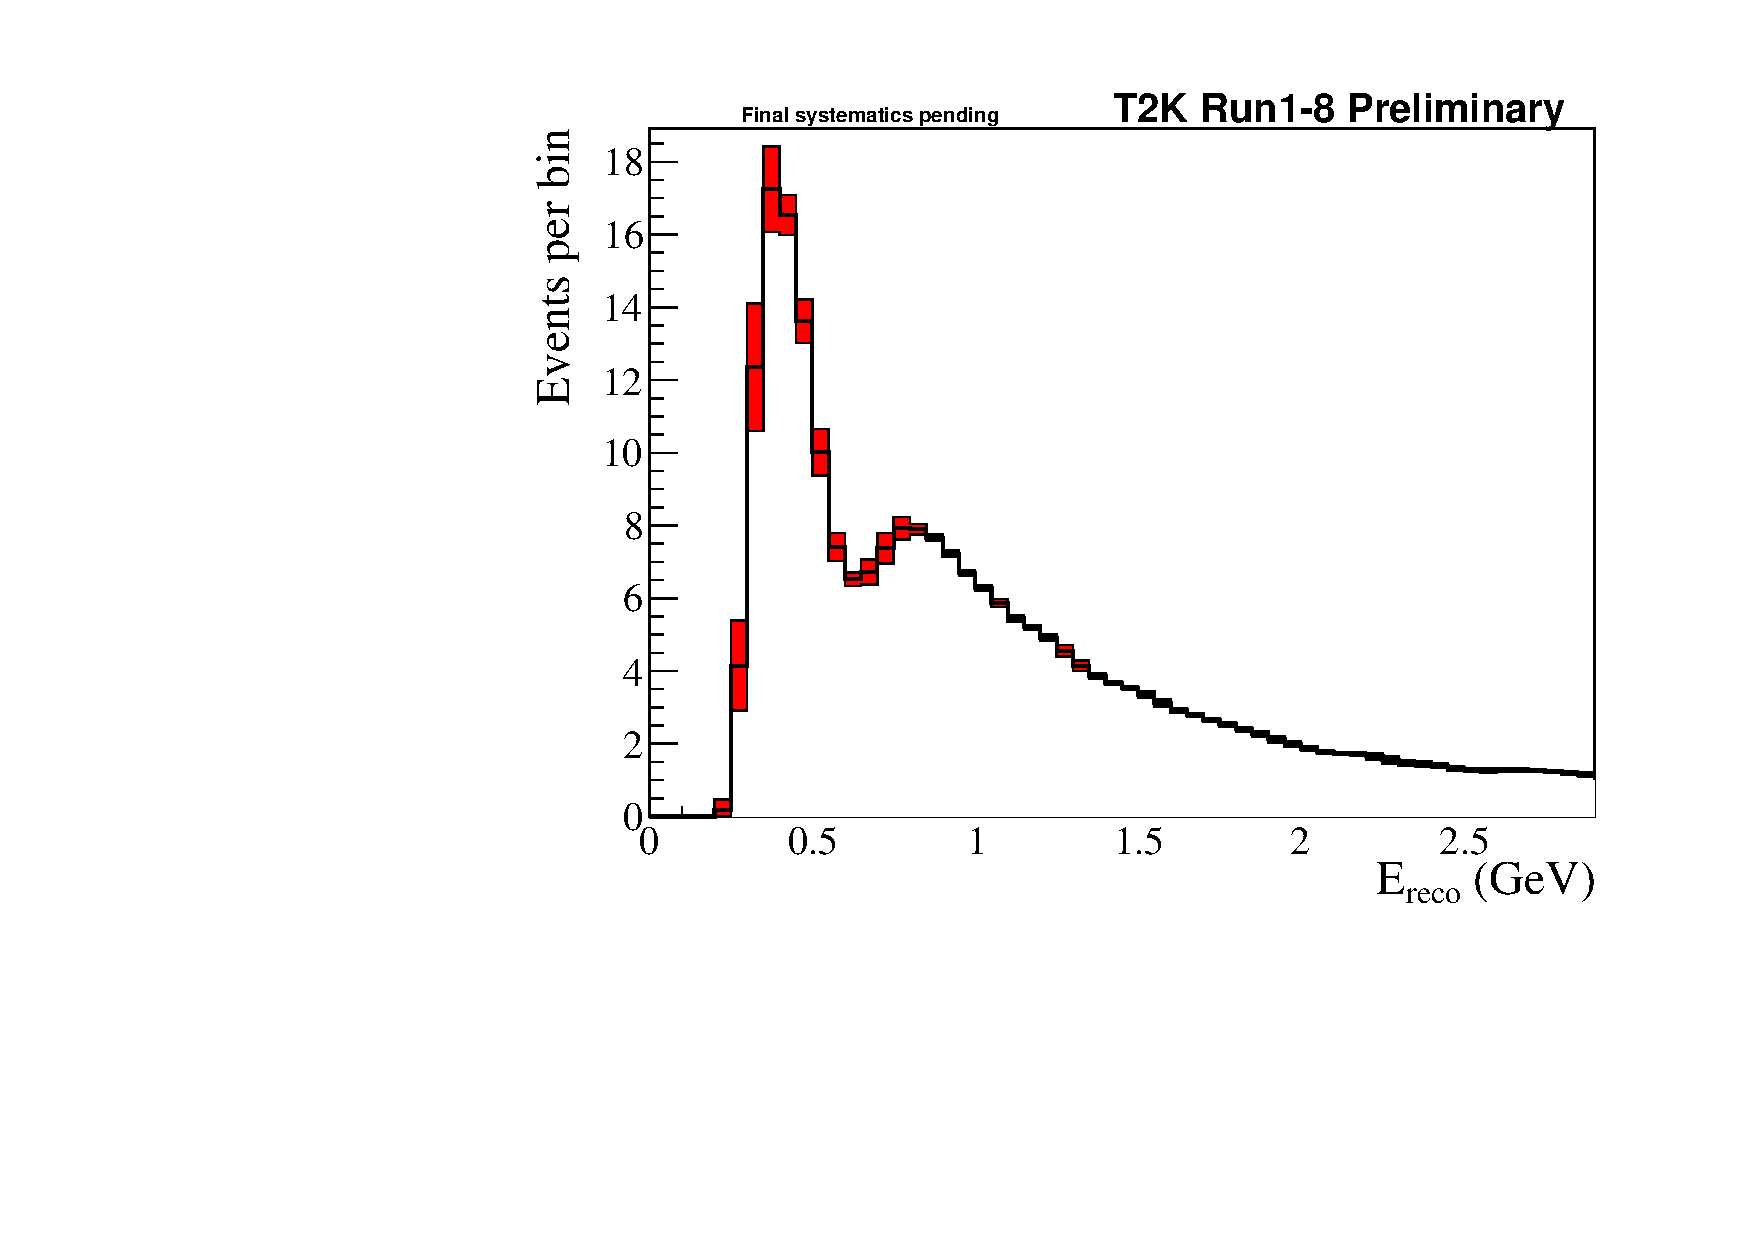
\includegraphics[width=0.9\textwidth]{systematics/envelopes/sk_errors/sk_error_table_1Rmu_skdet_envelope}
		\caption{Muon-like, neutrino mode}
	\end{subfigure}
	\begin{subfigure}[b]{0.49\textwidth}
		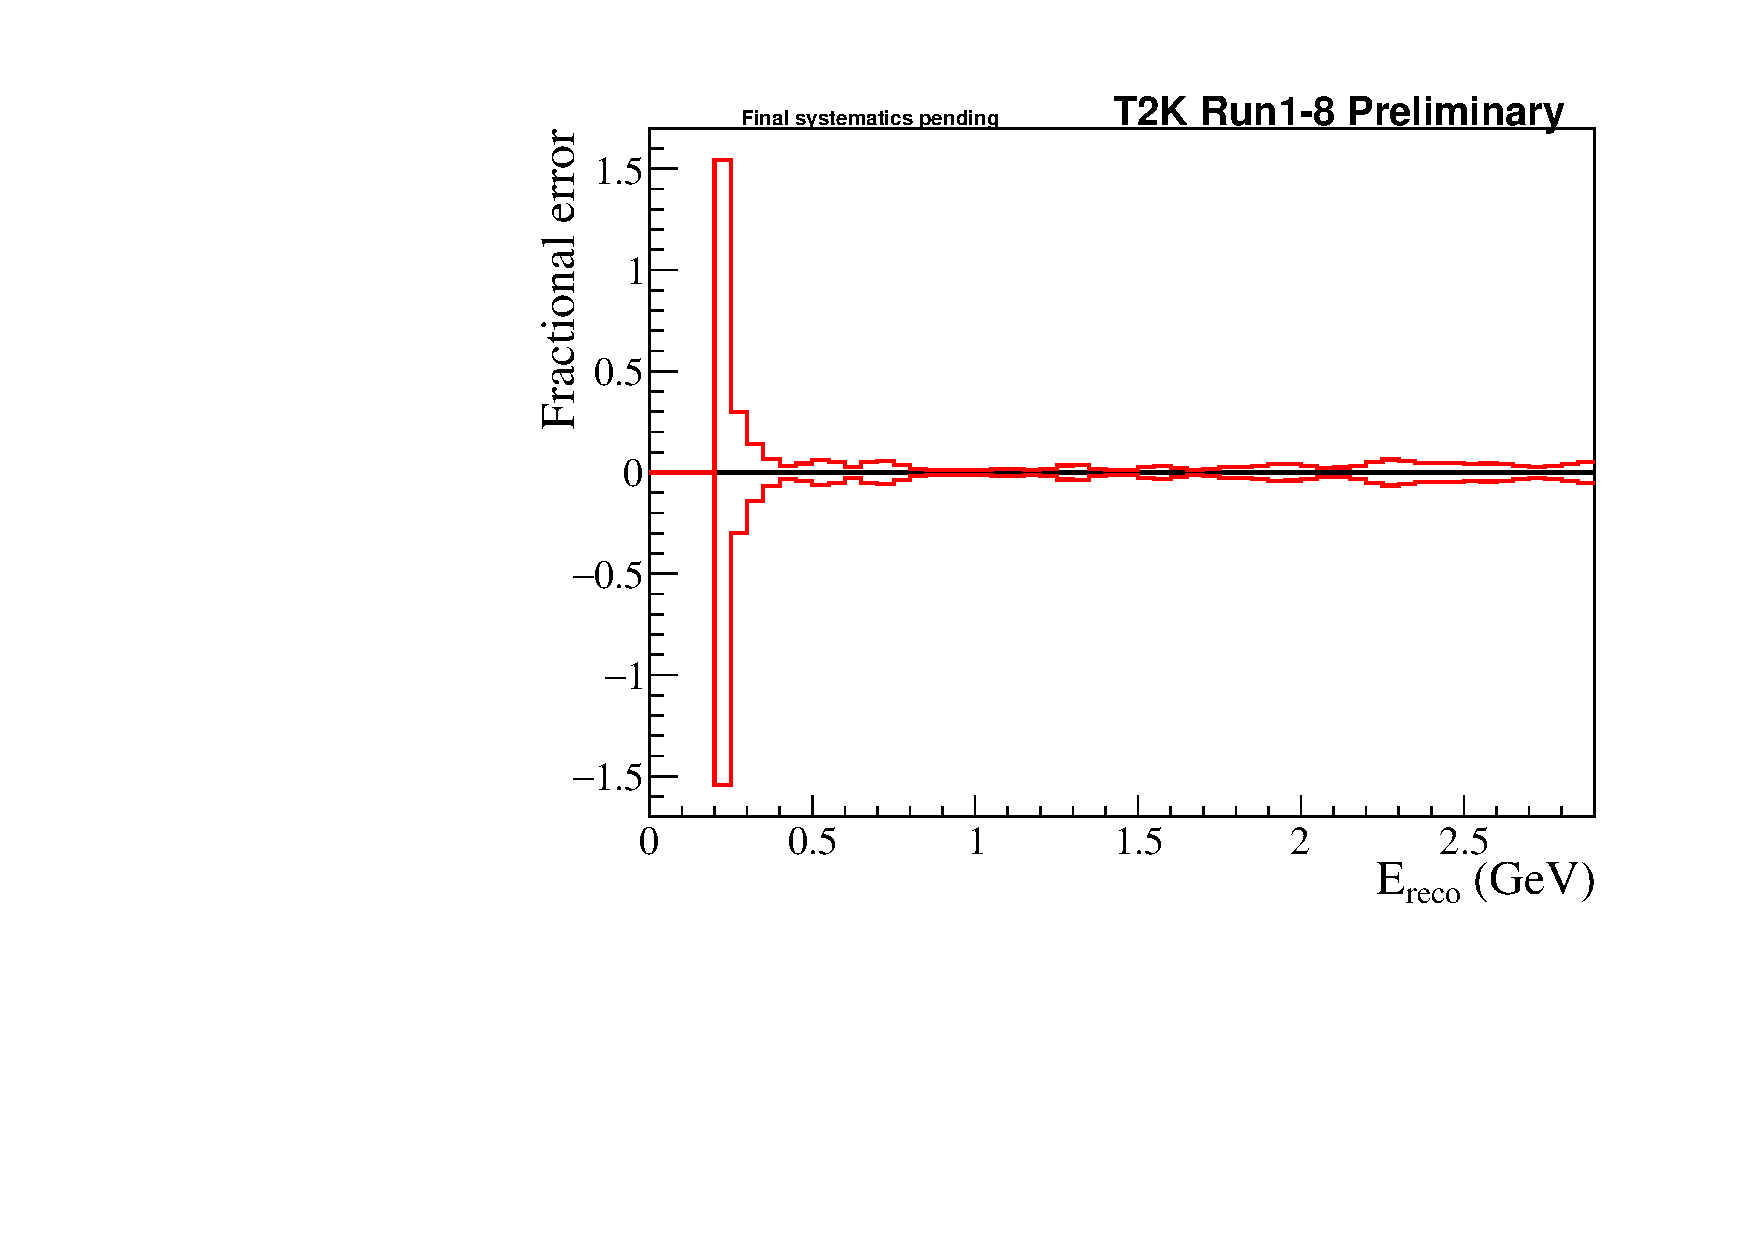
\includegraphics[width=0.9\textwidth]{systematics/envelopes/sk_errors/sk_error_table_1Rmu_skdet_envelope_fractional}
		\caption{Muon-like, neutrino mode}
	\end{subfigure}
	\begin{subfigure}[b]{0.49\textwidth}
		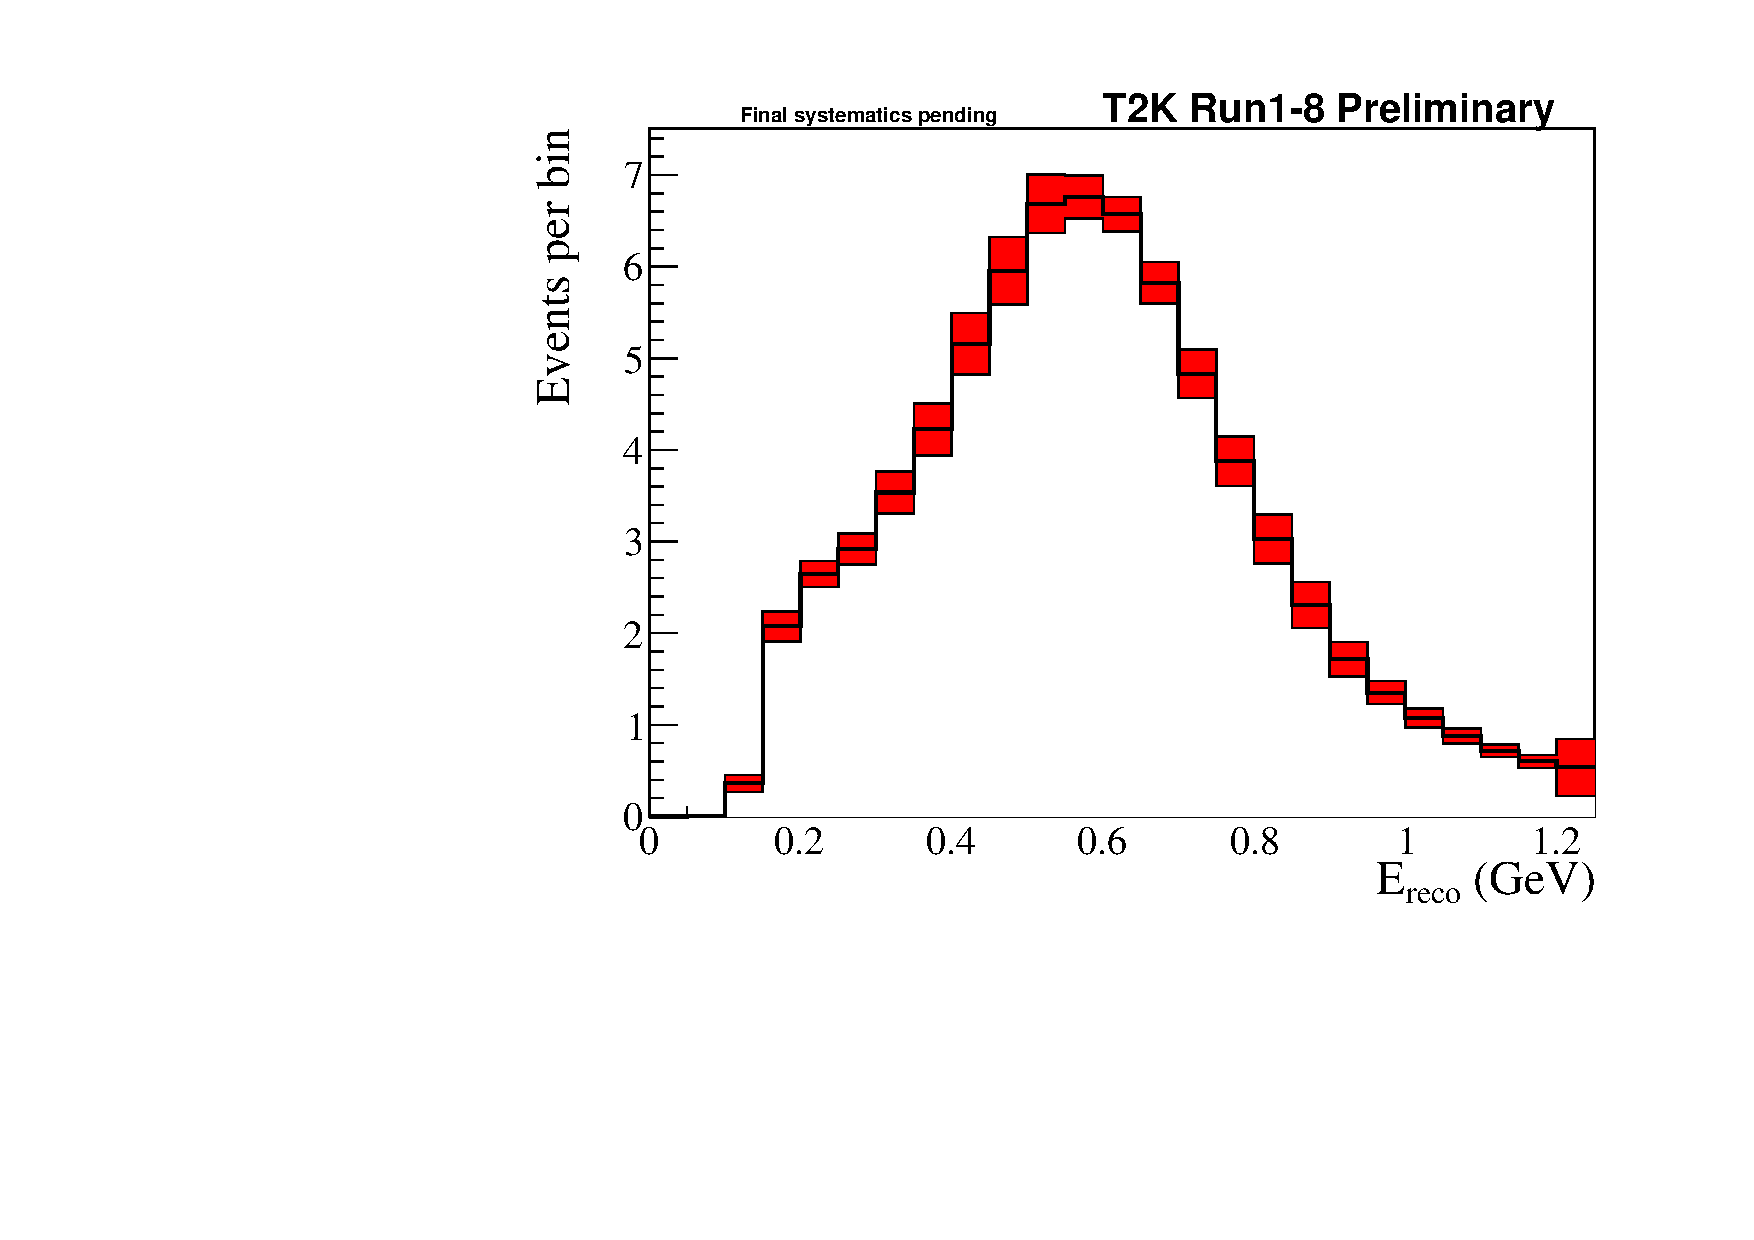
\includegraphics[width=0.9\textwidth]{systematics/envelopes/sk_errors/sk_error_table_1Re_skdet_envelope}
		\caption{Electron-like, neutrino mode}
	\end{subfigure}
	\begin{subfigure}[b]{0.49\textwidth}
		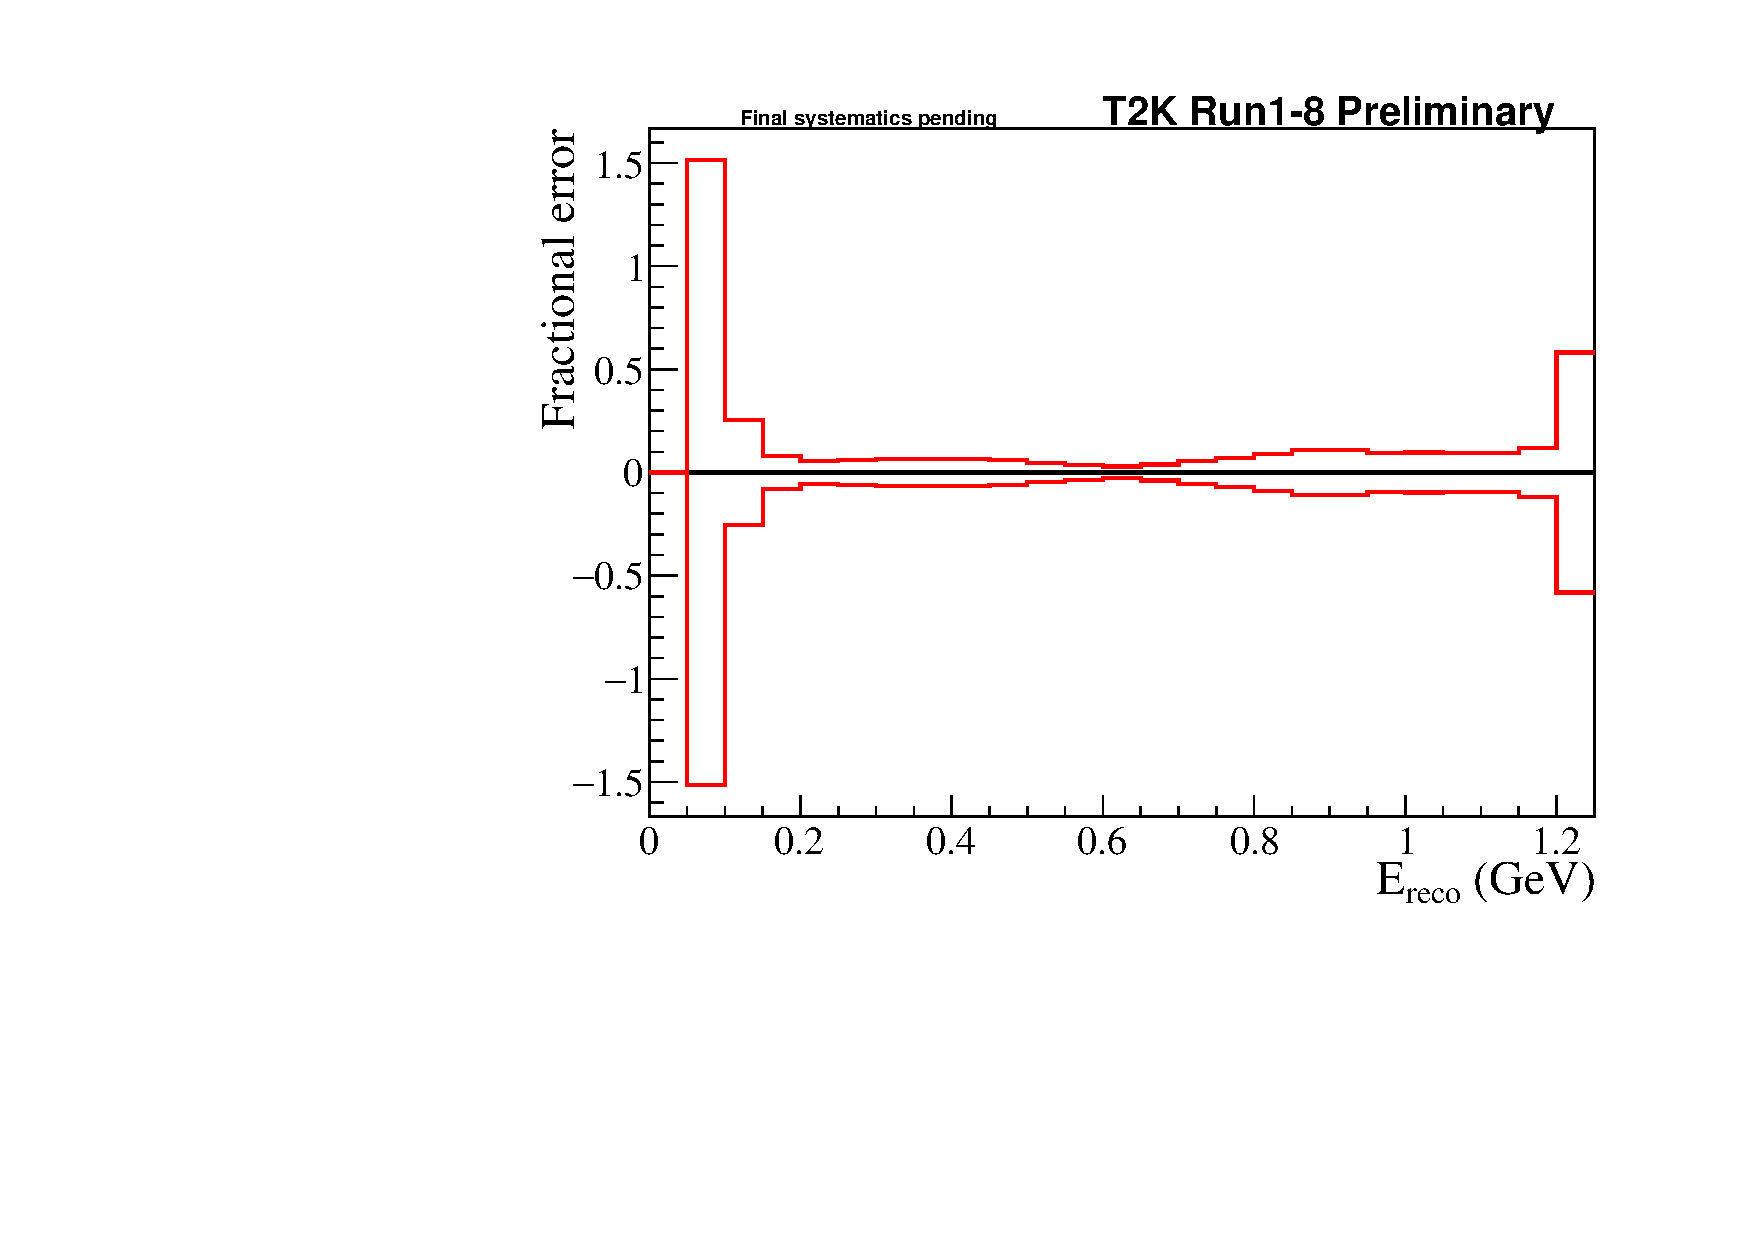
\includegraphics[width=0.9\textwidth]{systematics/envelopes/sk_errors/sk_error_table_1Re_skdet_envelope_fractional}
		\caption{Electron-like, neutrino mode}
	\end{subfigure}
	\begin{subfigure}[b]{0.49\textwidth}
		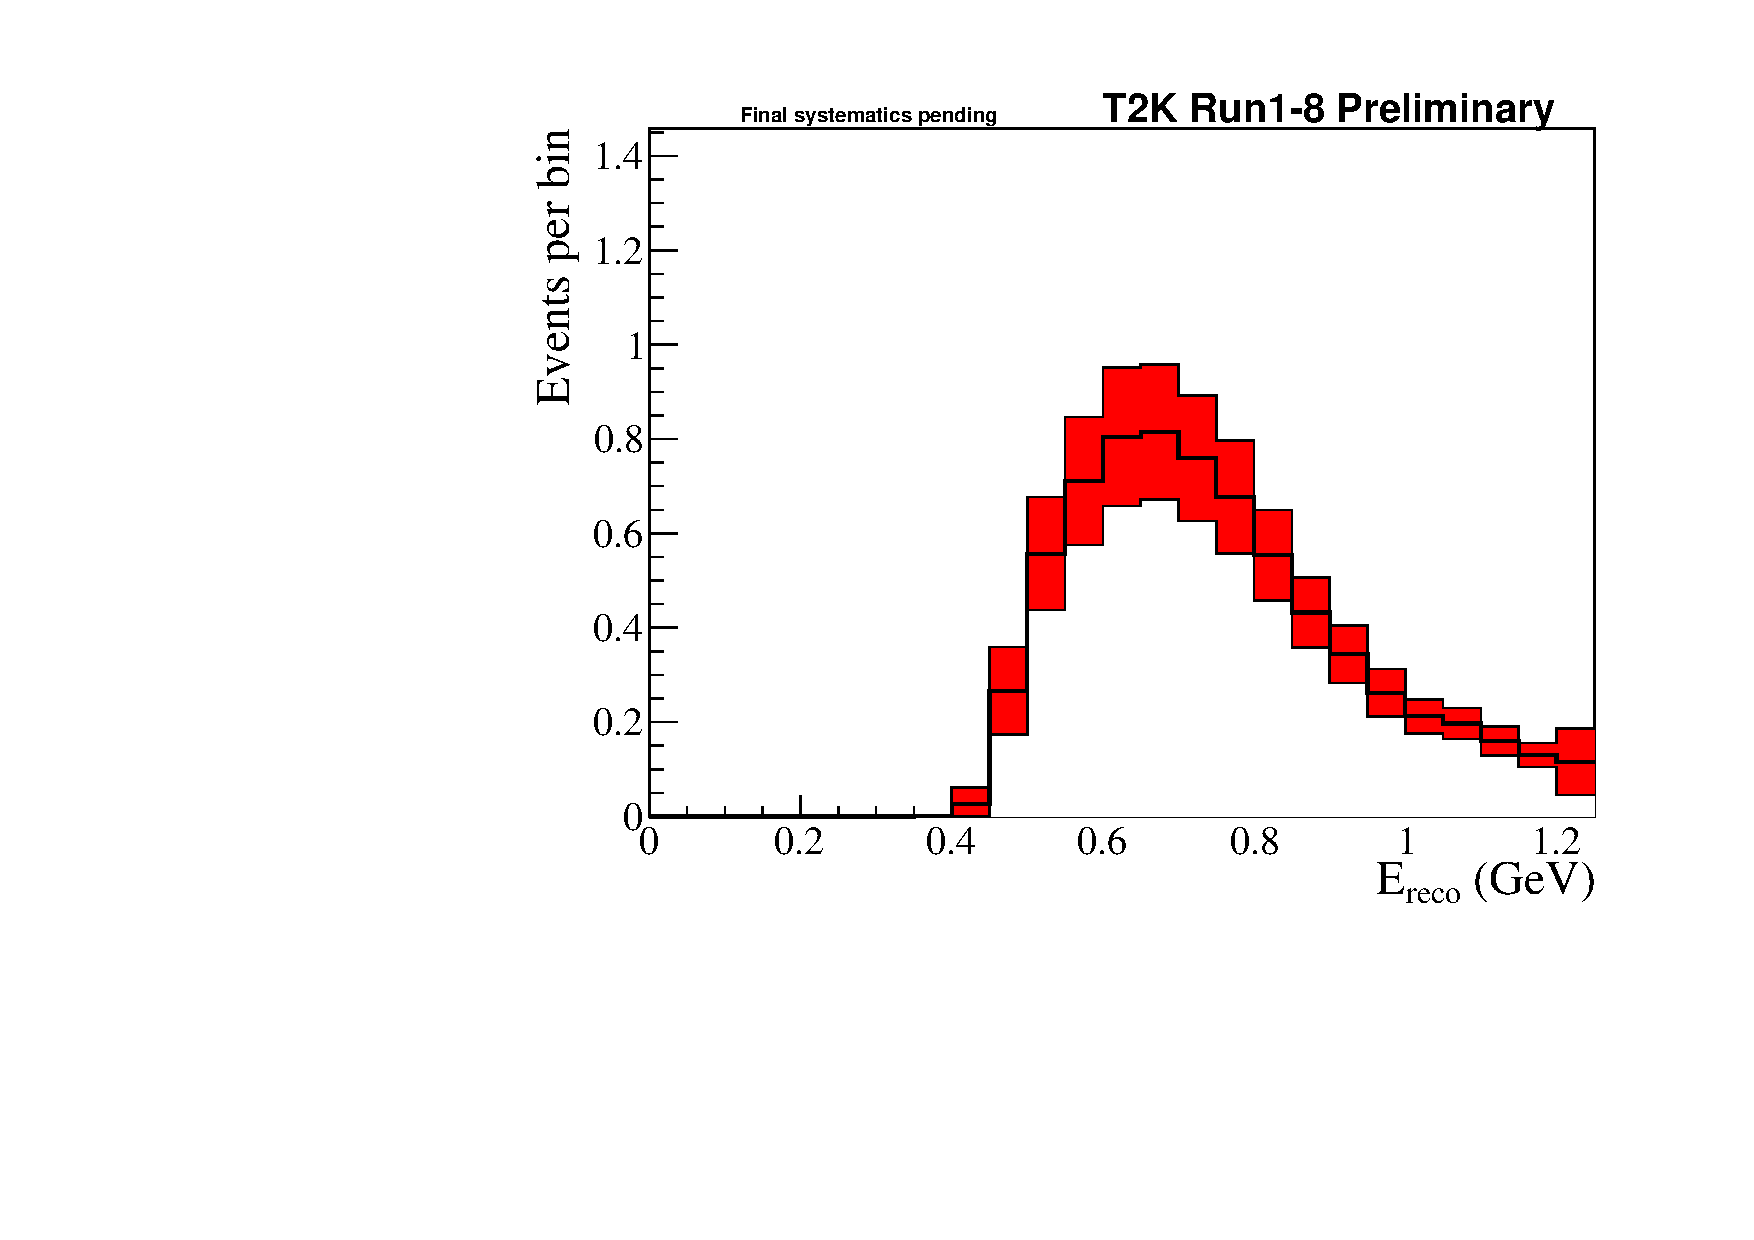
\includegraphics[width=0.9\textwidth]{systematics/envelopes/sk_errors/sk_error_table_MultiRe_skdet_envelope}
		\caption{\nueCConepi-like, neutrino mode}
	\end{subfigure}
	\begin{subfigure}[b]{0.49\textwidth}
		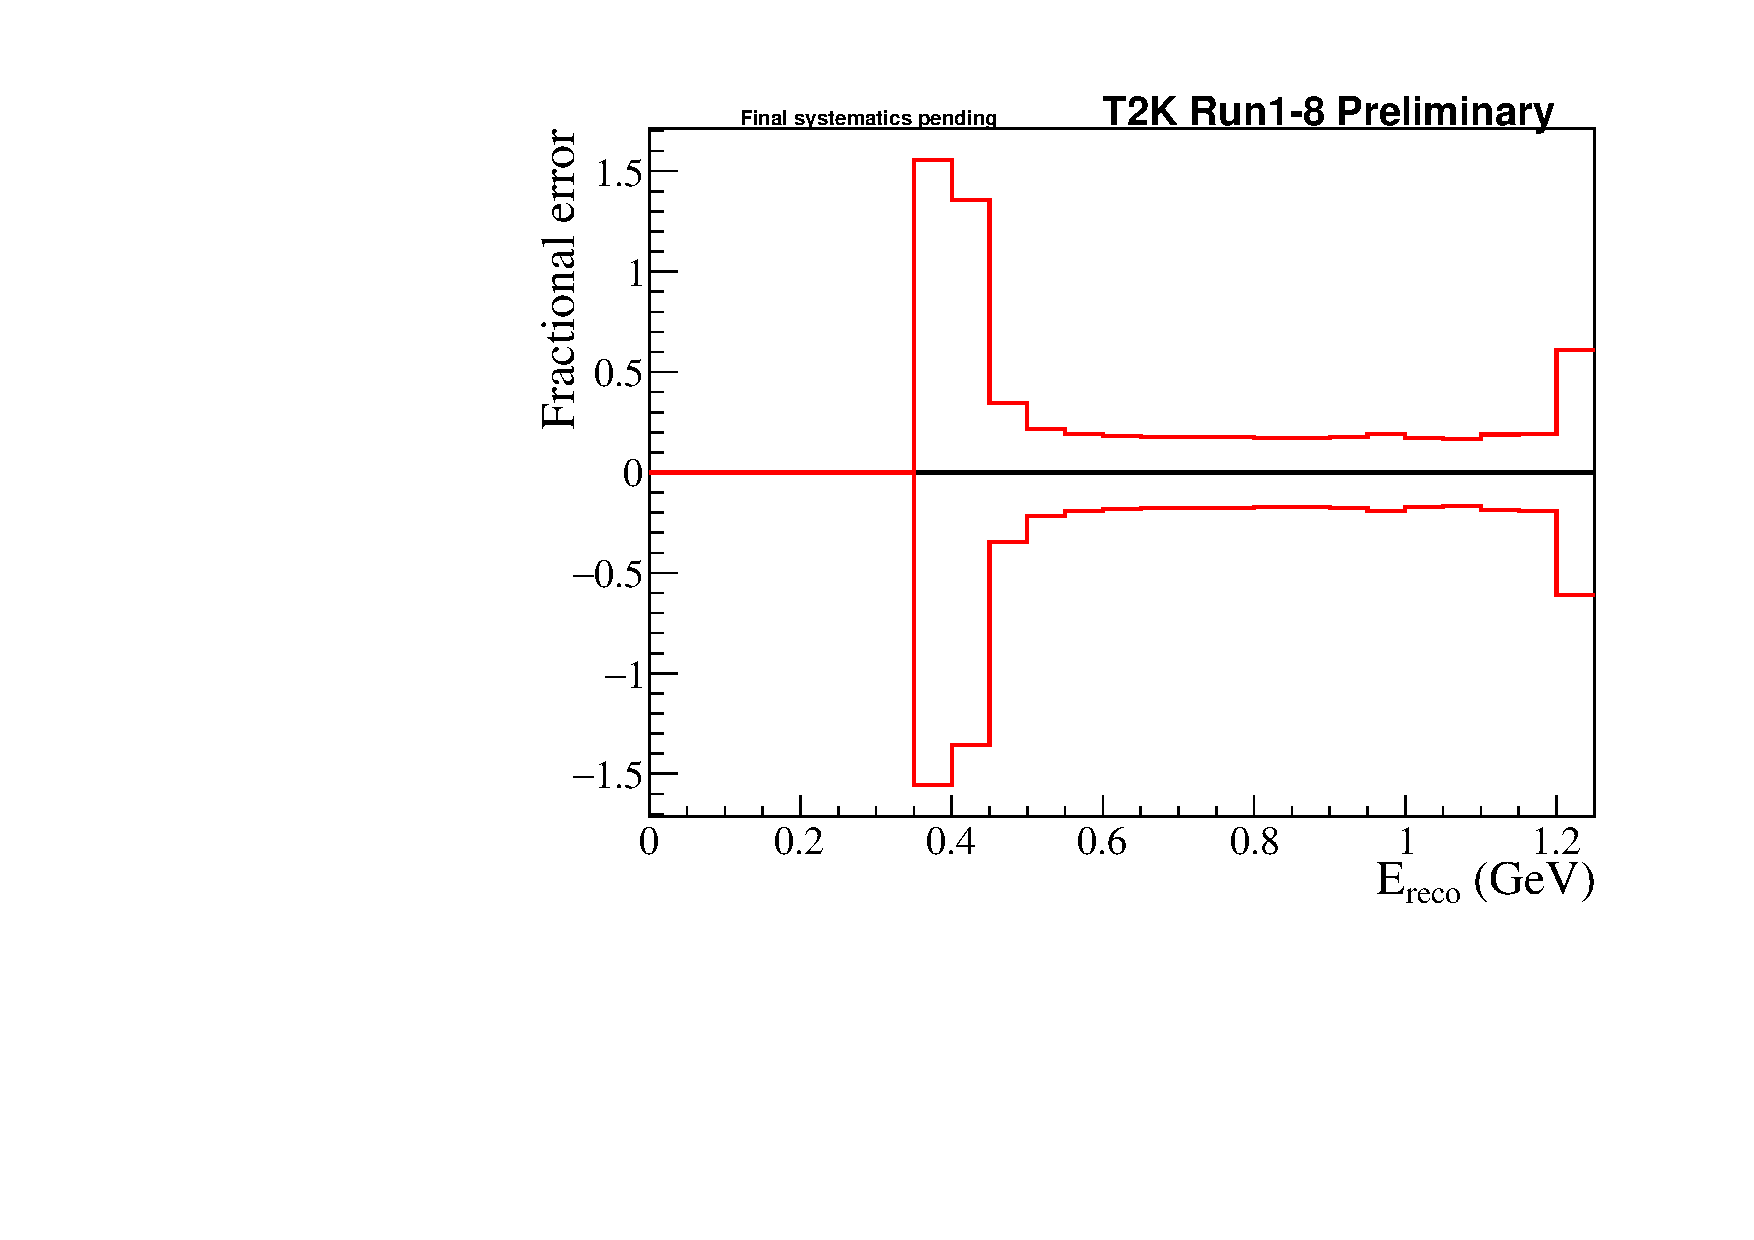
\includegraphics[width=0.9\textwidth]{systematics/envelopes/sk_errors/sk_error_table_MultiRe_skdet_envelope_fractional}
		\caption{\nueCConepi-like, neutrino mode}
	\end{subfigure}
	\caption {
		Error envelopes (left) and fractional error (right) for the reconstructed neutrino energy spectrum for Super-K detector systematic parameters. \num{1e4} toys are generated for the Asimov data set A with randomized systematic parameters with correlations taken into account.
	}
	\label{fig:sk_envelopes_skdet}
\end{figure*}
\clearpage

\begin{figure*}
	\center
	\begin{subfigure}[b]{0.49\textwidth}
		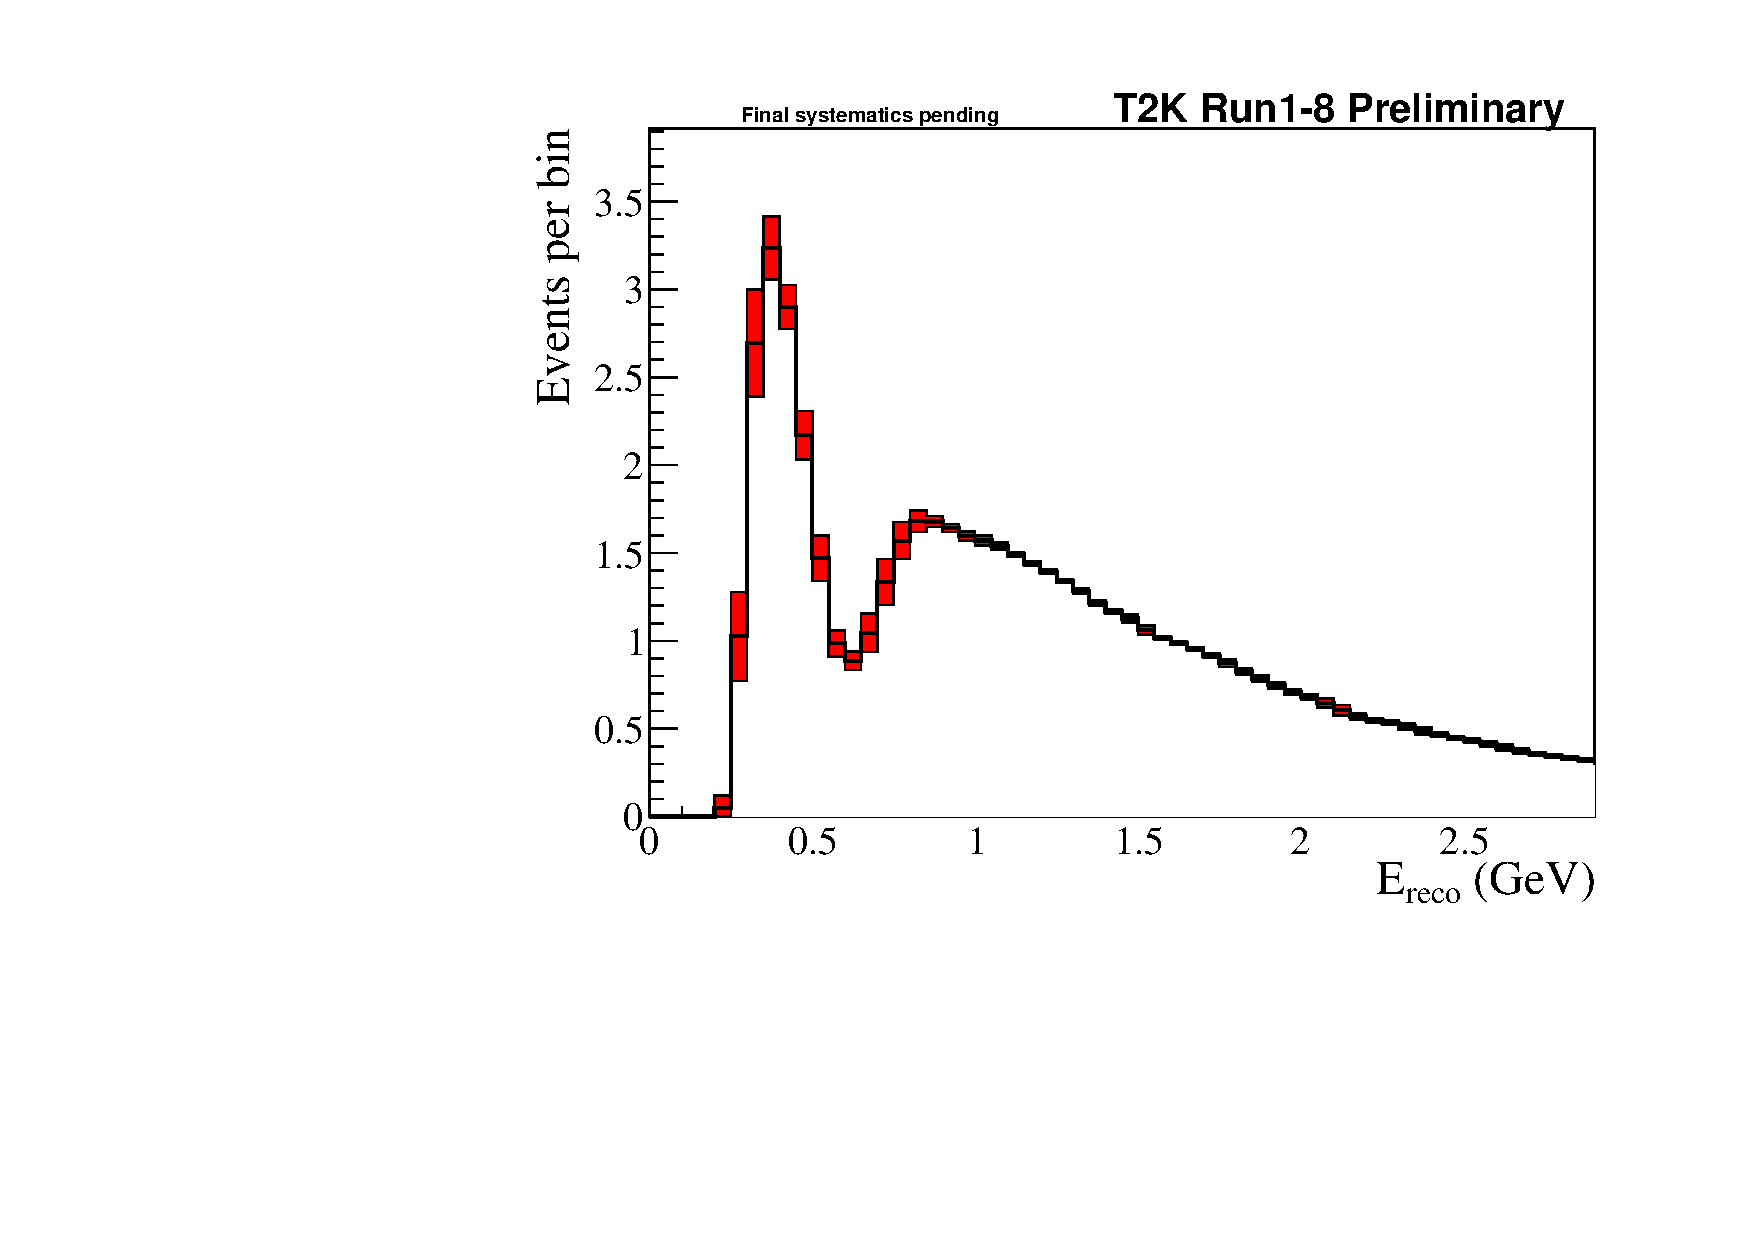
\includegraphics[width=0.9\textwidth]{systematics/envelopes/sk_errors/sk_error_table_RHC1Rmu_skdet_envelope}
		\caption{Muon-like, antineutrino mode}
	\end{subfigure}
	\begin{subfigure}[b]{0.49\textwidth}
		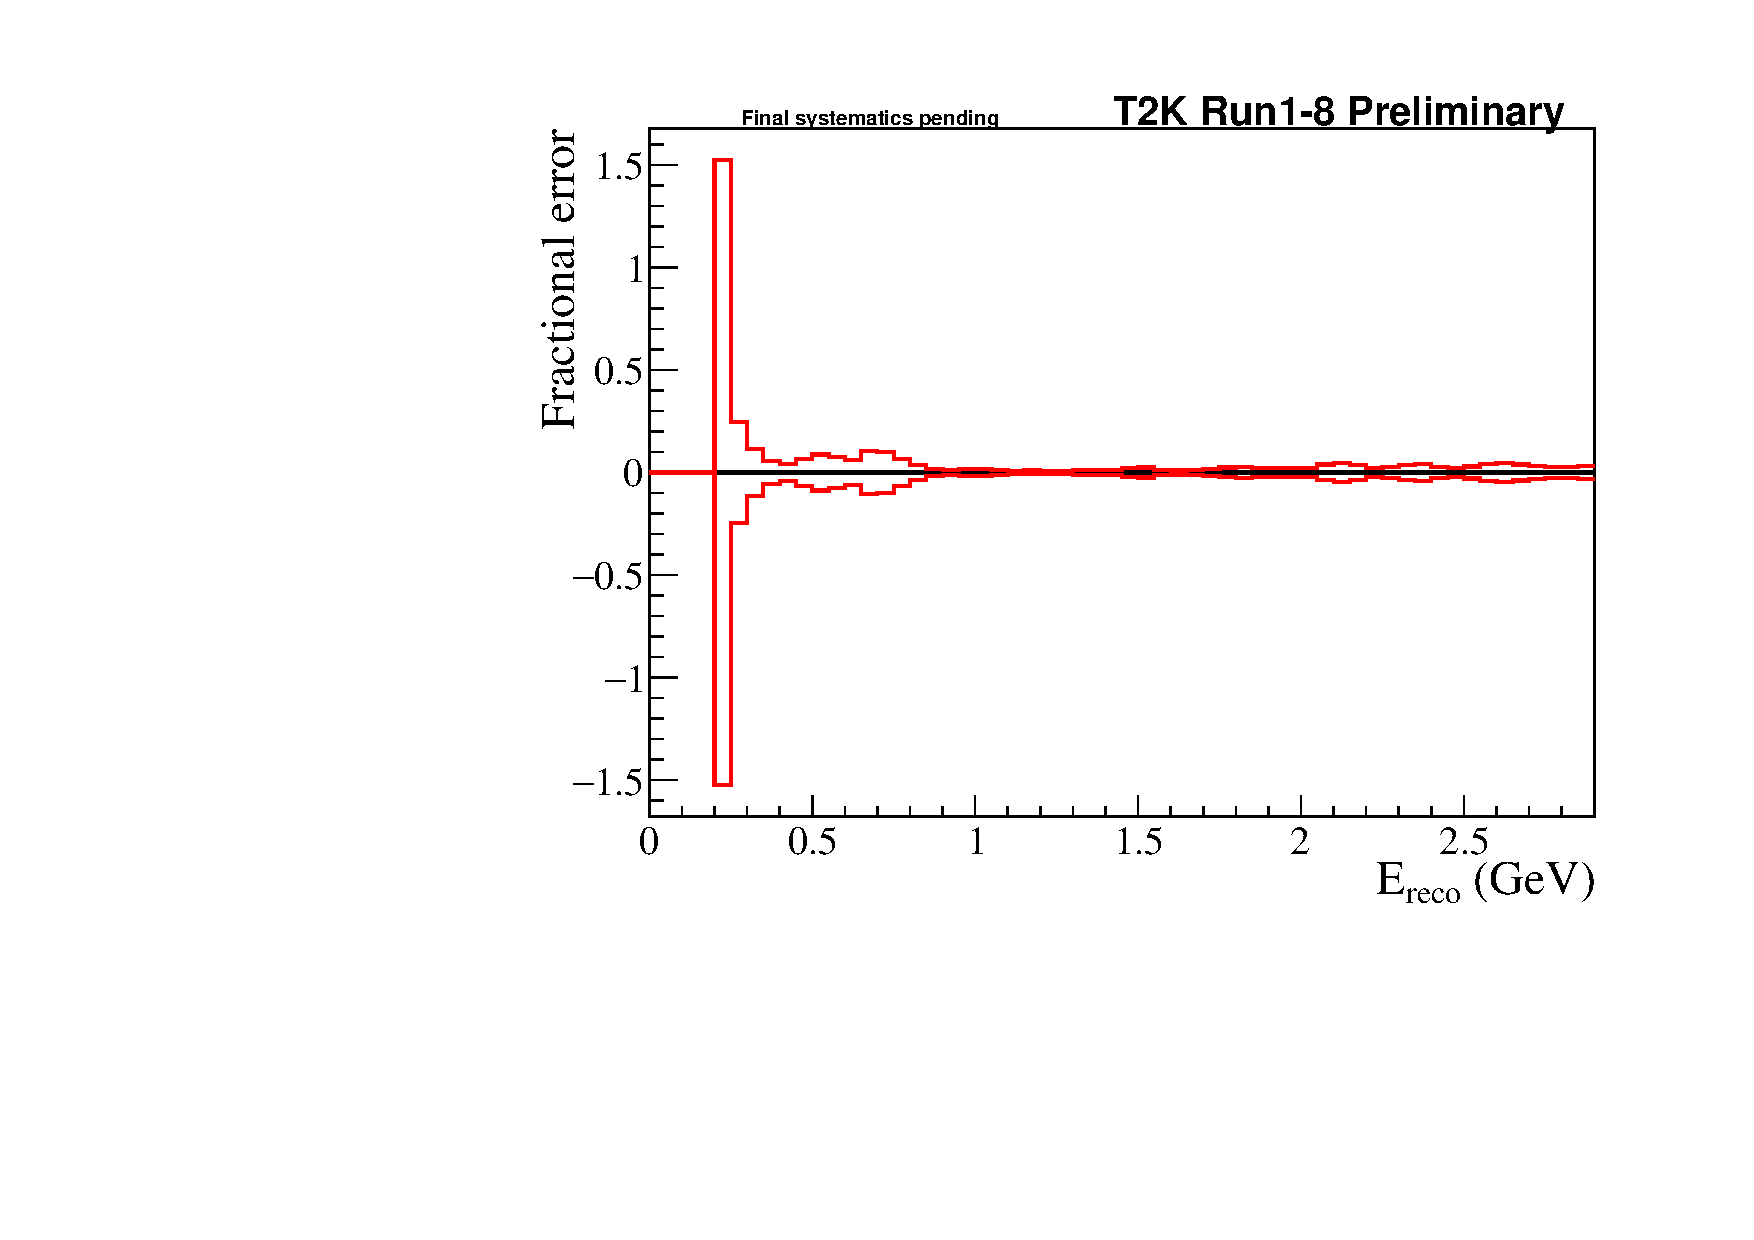
\includegraphics[width=0.9\textwidth]{systematics/envelopes/sk_errors/sk_error_table_RHC1Rmu_skdet_envelope_fractional}
		\caption{Muon-like, antineutrino mode}
	\end{subfigure}
	\begin{subfigure}[b]{0.49\textwidth}
		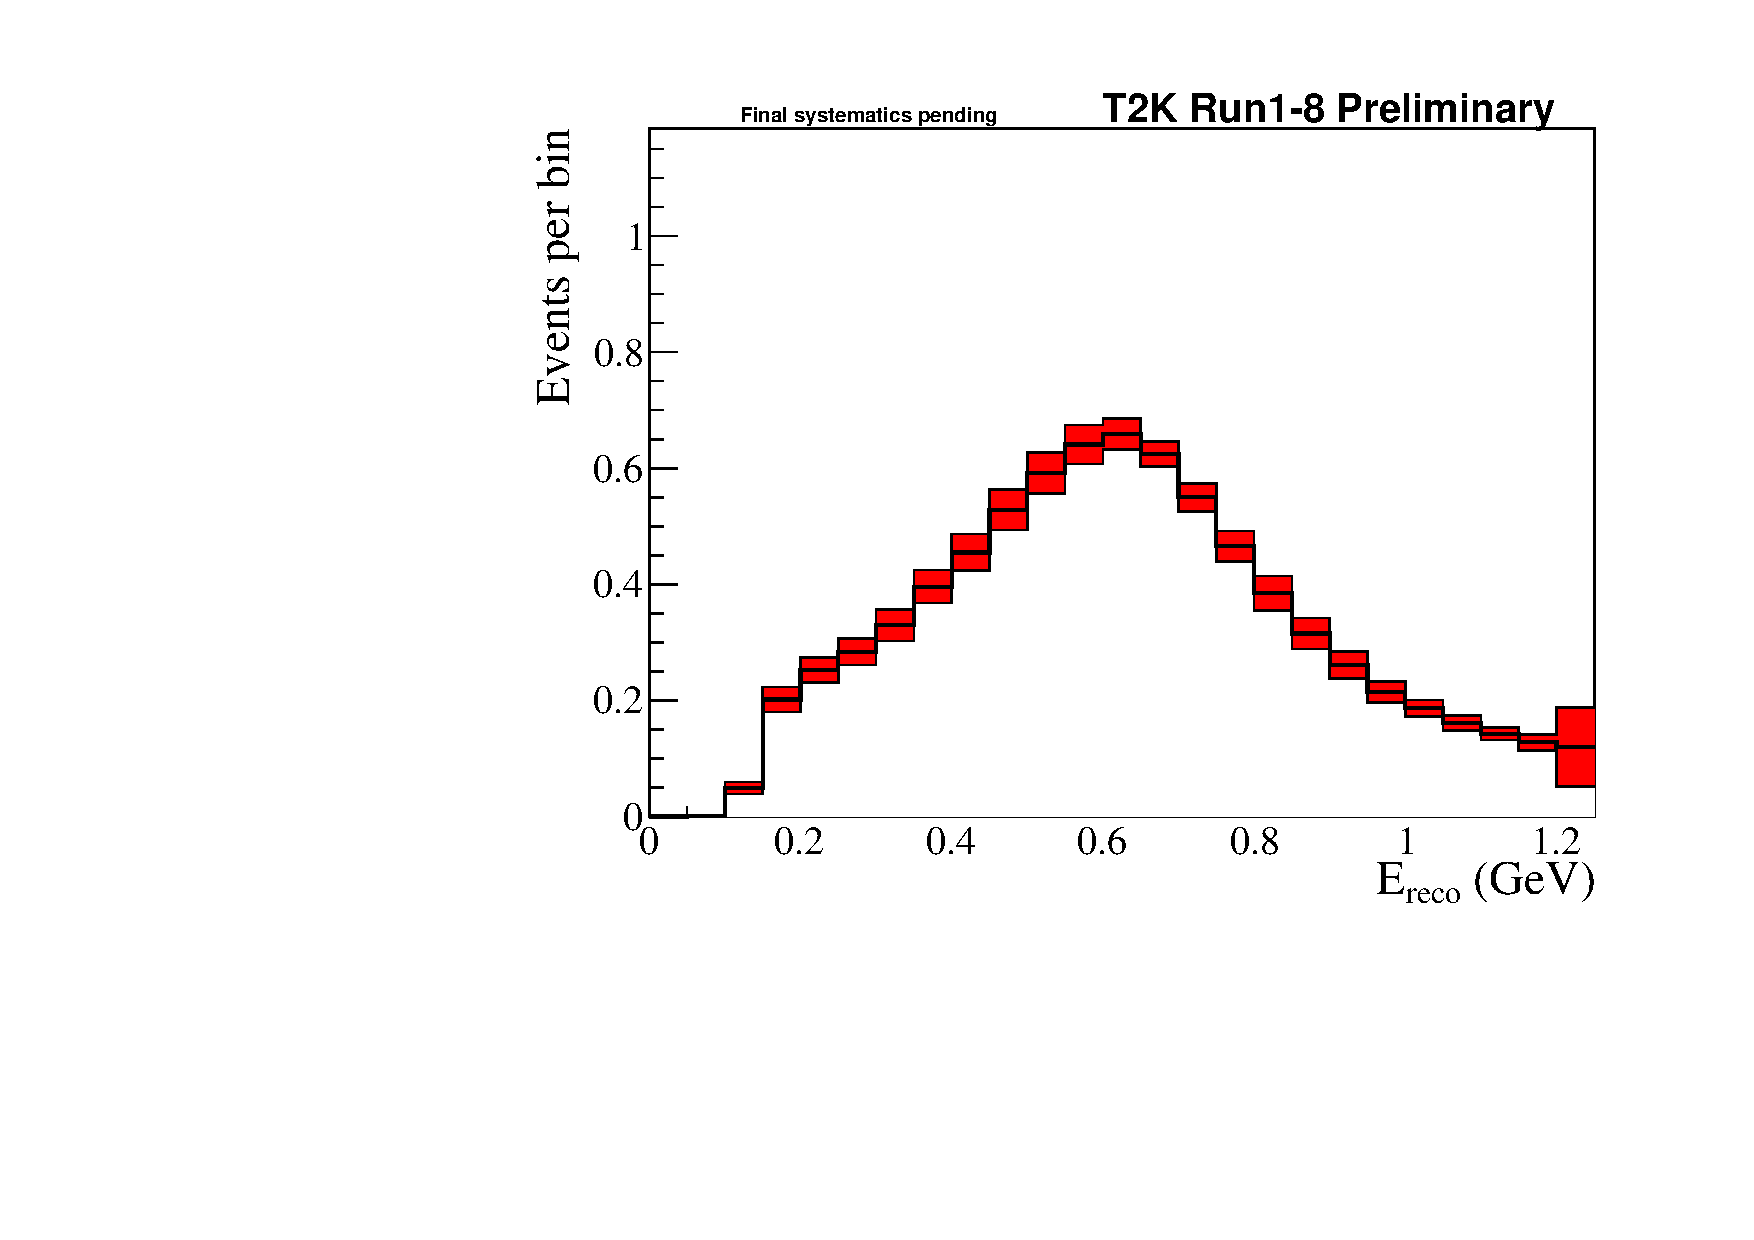
\includegraphics[width=0.9\textwidth]{systematics/envelopes/sk_errors/sk_error_table_RHC1Re_skdet_envelope}
		\caption{Electron-like antineutrino mode}
	\end{subfigure}
	\begin{subfigure}[b]{0.49\textwidth}
		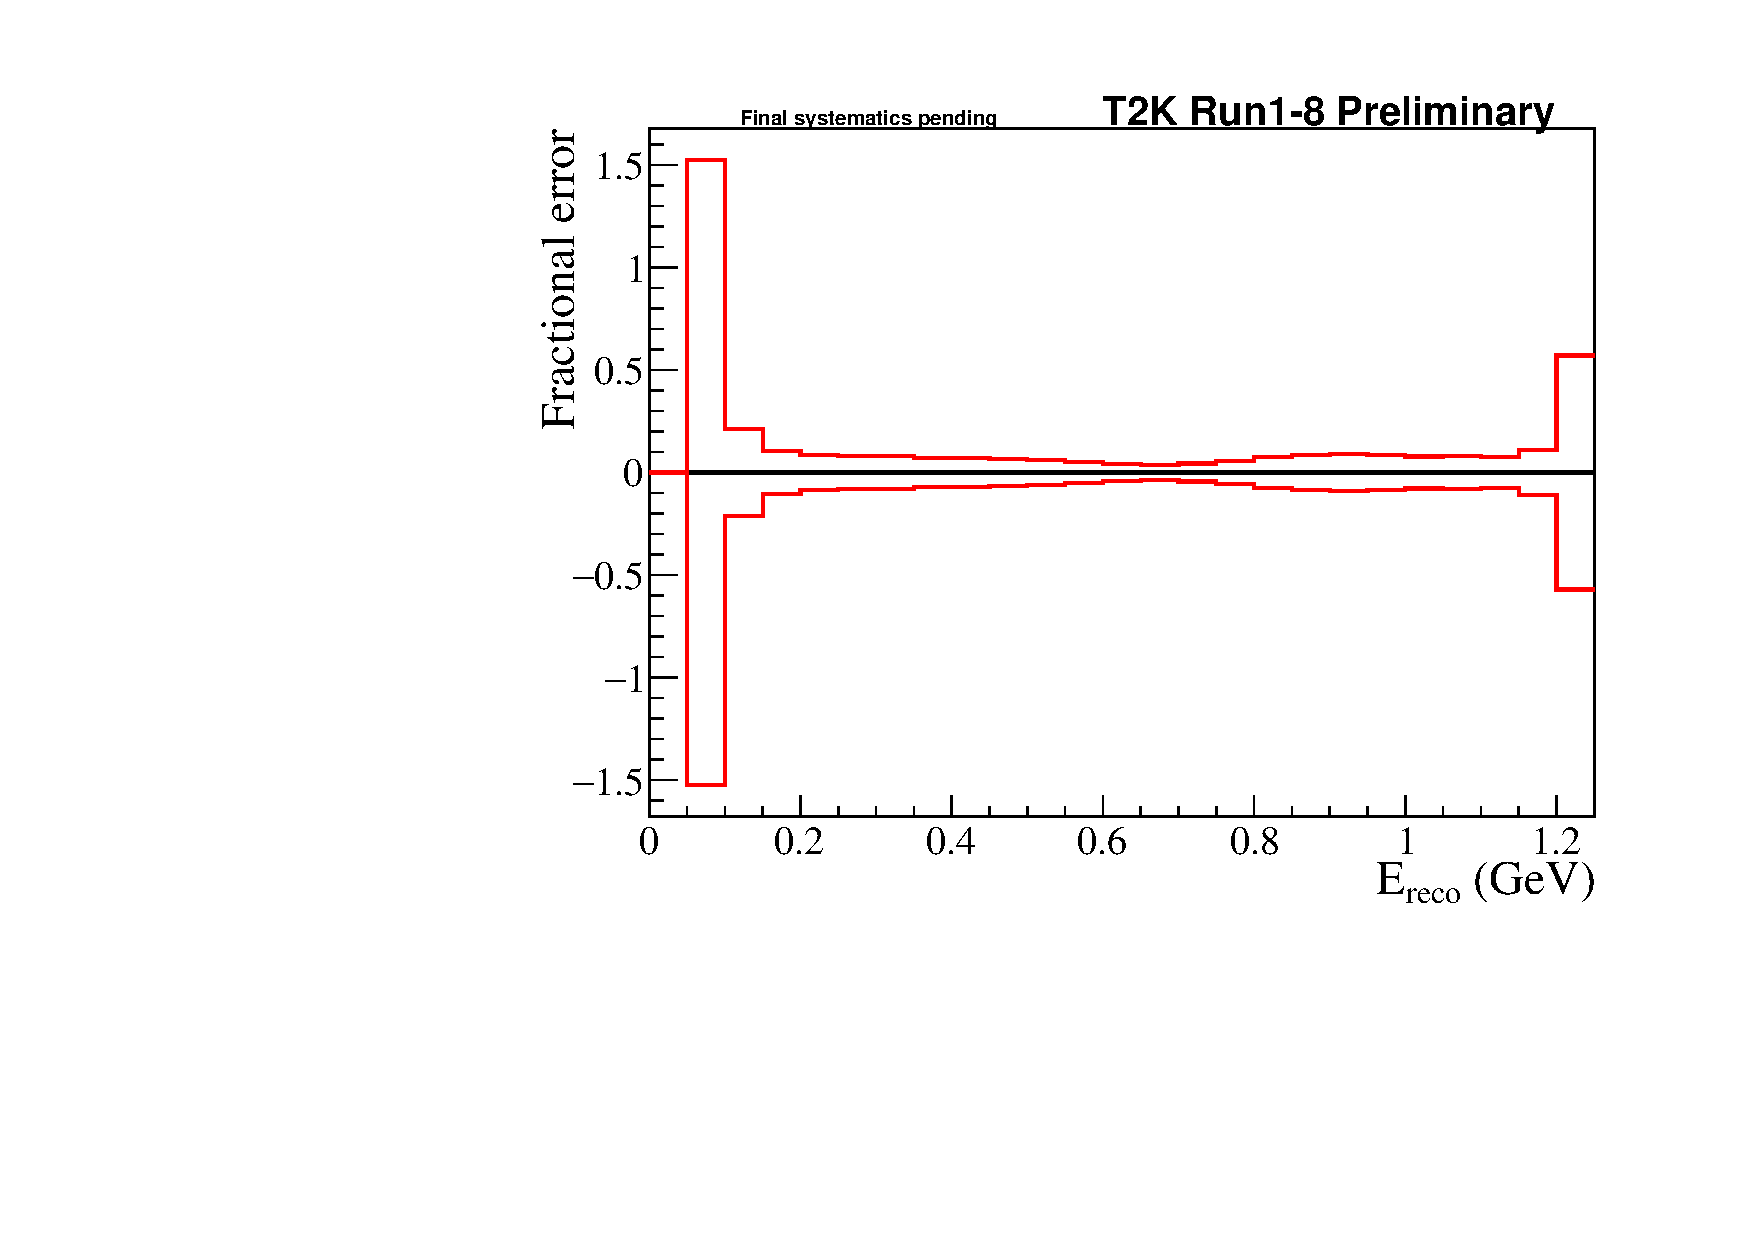
\includegraphics[width=0.9\textwidth]{systematics/envelopes/sk_errors/sk_error_table_RHC1Re_skdet_envelope_fractional}
		\caption{Electron-like antineutrino mode}
	\end{subfigure}
	\caption {
		Error envelopes (left) and fractional error (right) for the reconstructed neutrino energy spectrum for Super-K detector systematic parameters. \num{1e4} toys are generated for the Asimov data set A with randomized systematic parameters with correlations taken into account.
	}
	\label{fig:sk_envelopes_skdet_b}
\end{figure*}
\clearpage
\begin{figure*}
	\center
	\begin{subfigure}[b]{0.49\textwidth}
		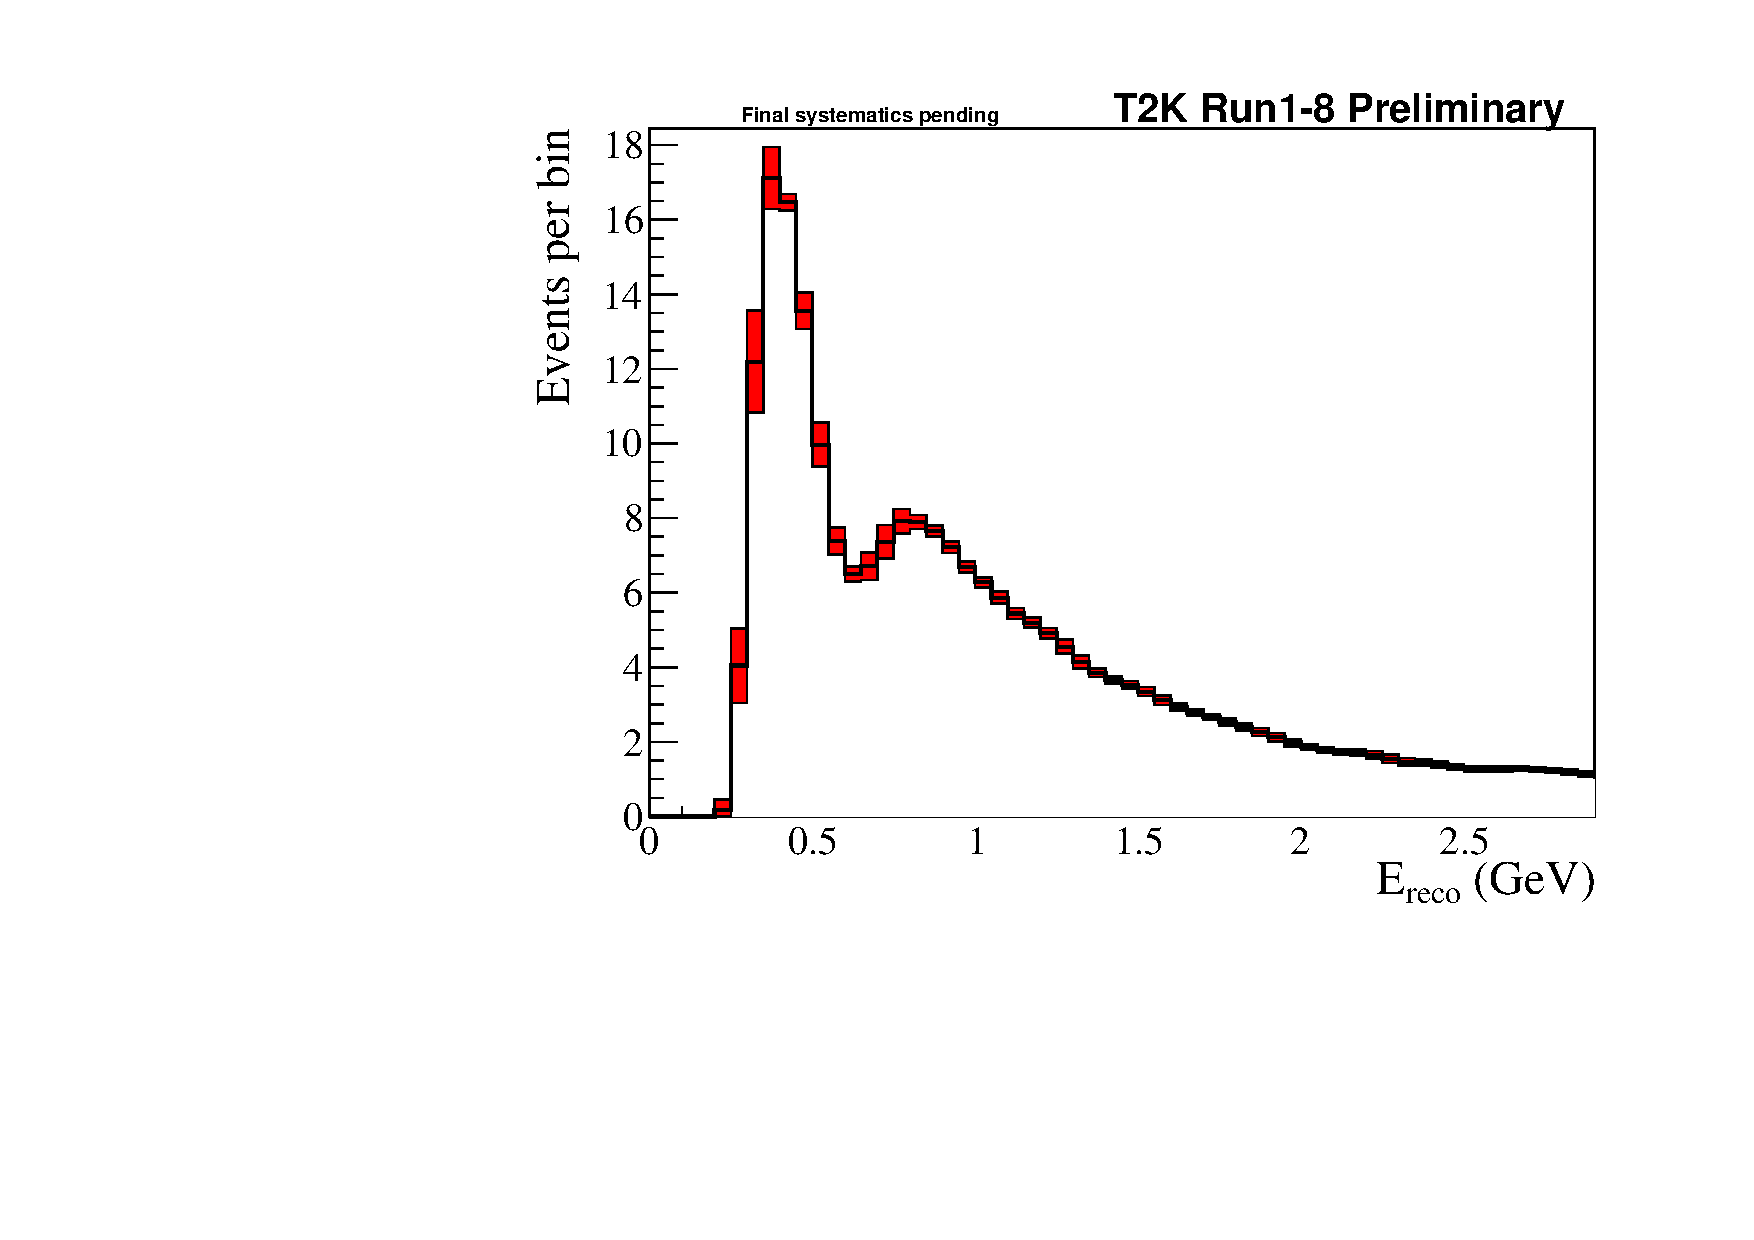
\includegraphics[width=0.9\textwidth]{systematics/envelopes/sk_errors/sk_error_table_1Rmu_skfsi_envelope}
		\caption{Muon-like, neutrino mode}
	\end{subfigure}
	\begin{subfigure}[b]{0.49\textwidth}
		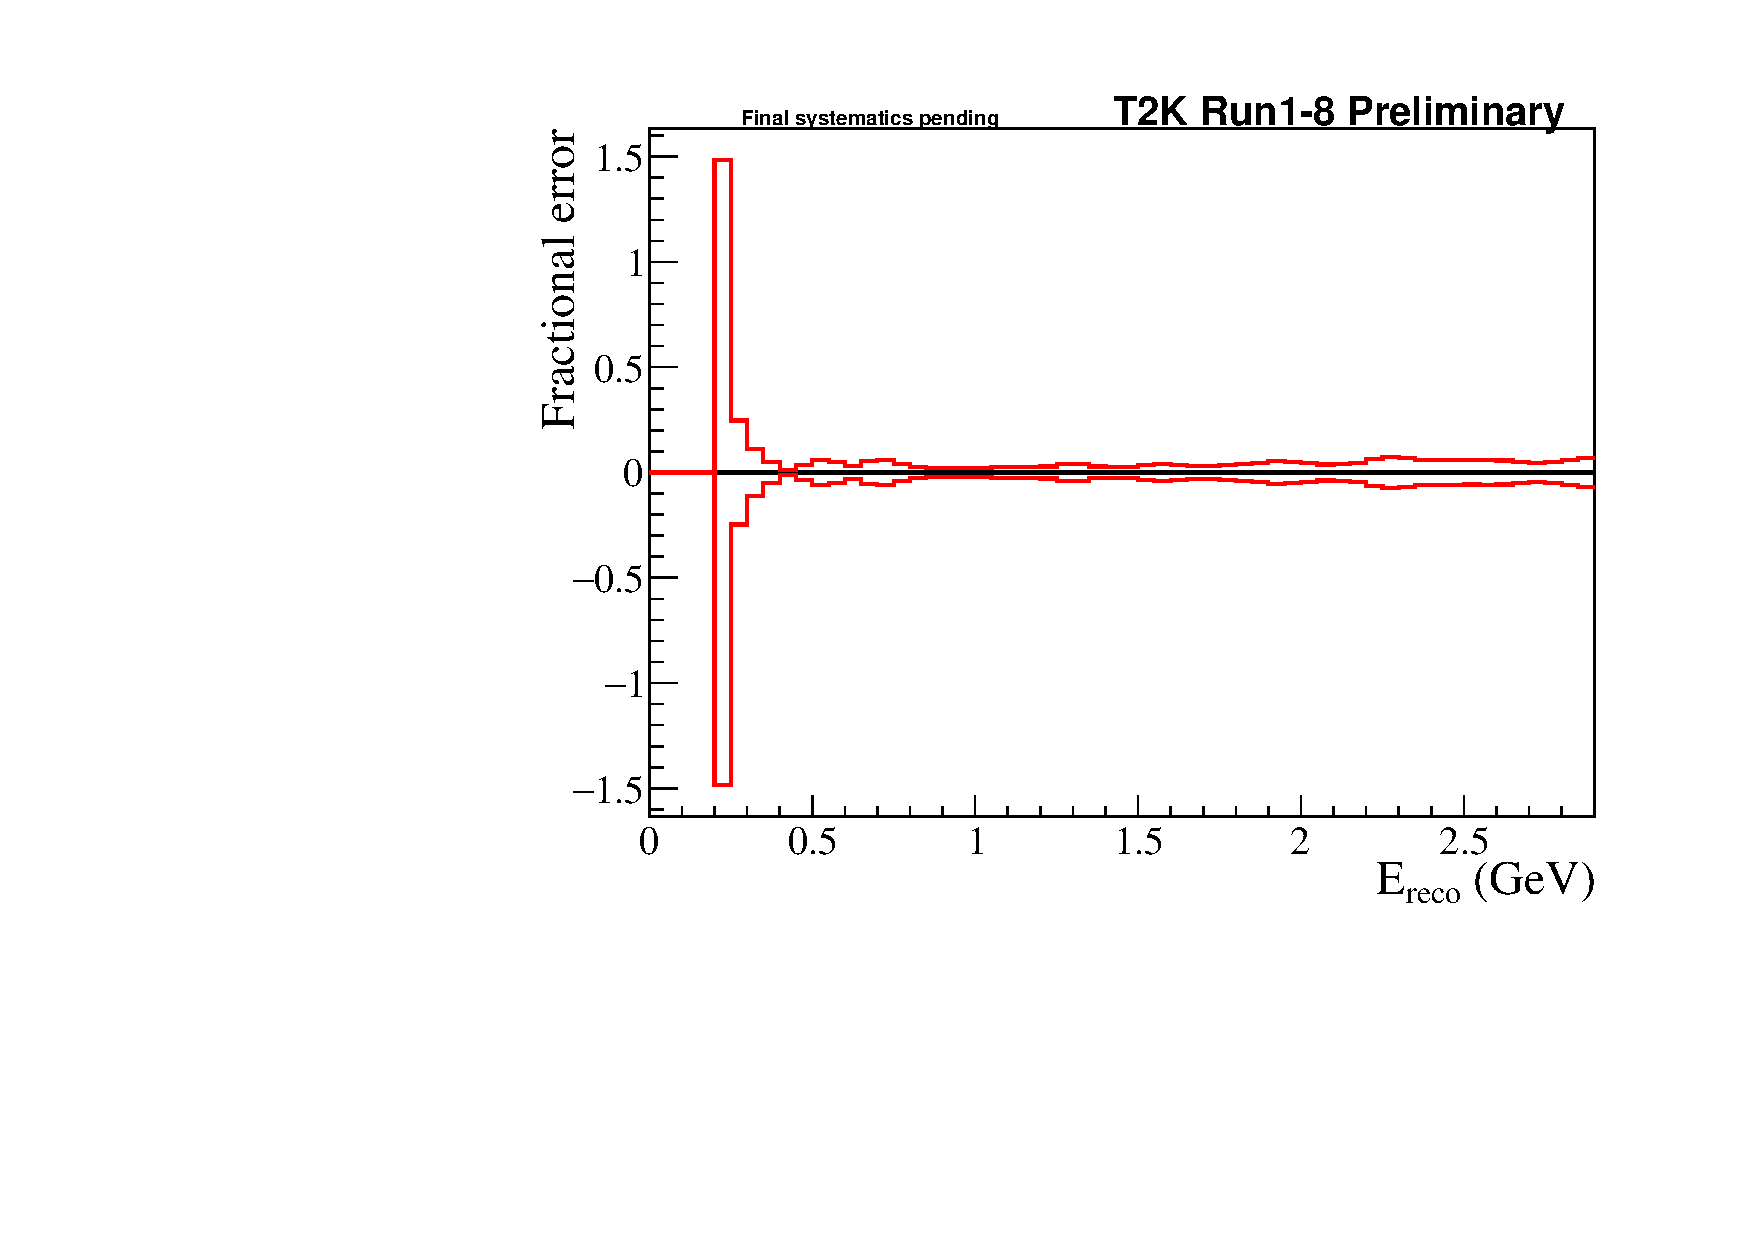
\includegraphics[width=0.9\textwidth]{systematics/envelopes/sk_errors/sk_error_table_1Rmu_skfsi_envelope_fractional}
		\caption{Muon-like, neutrino mode}
	\end{subfigure}
	\begin{subfigure}[b]{0.49\textwidth}
		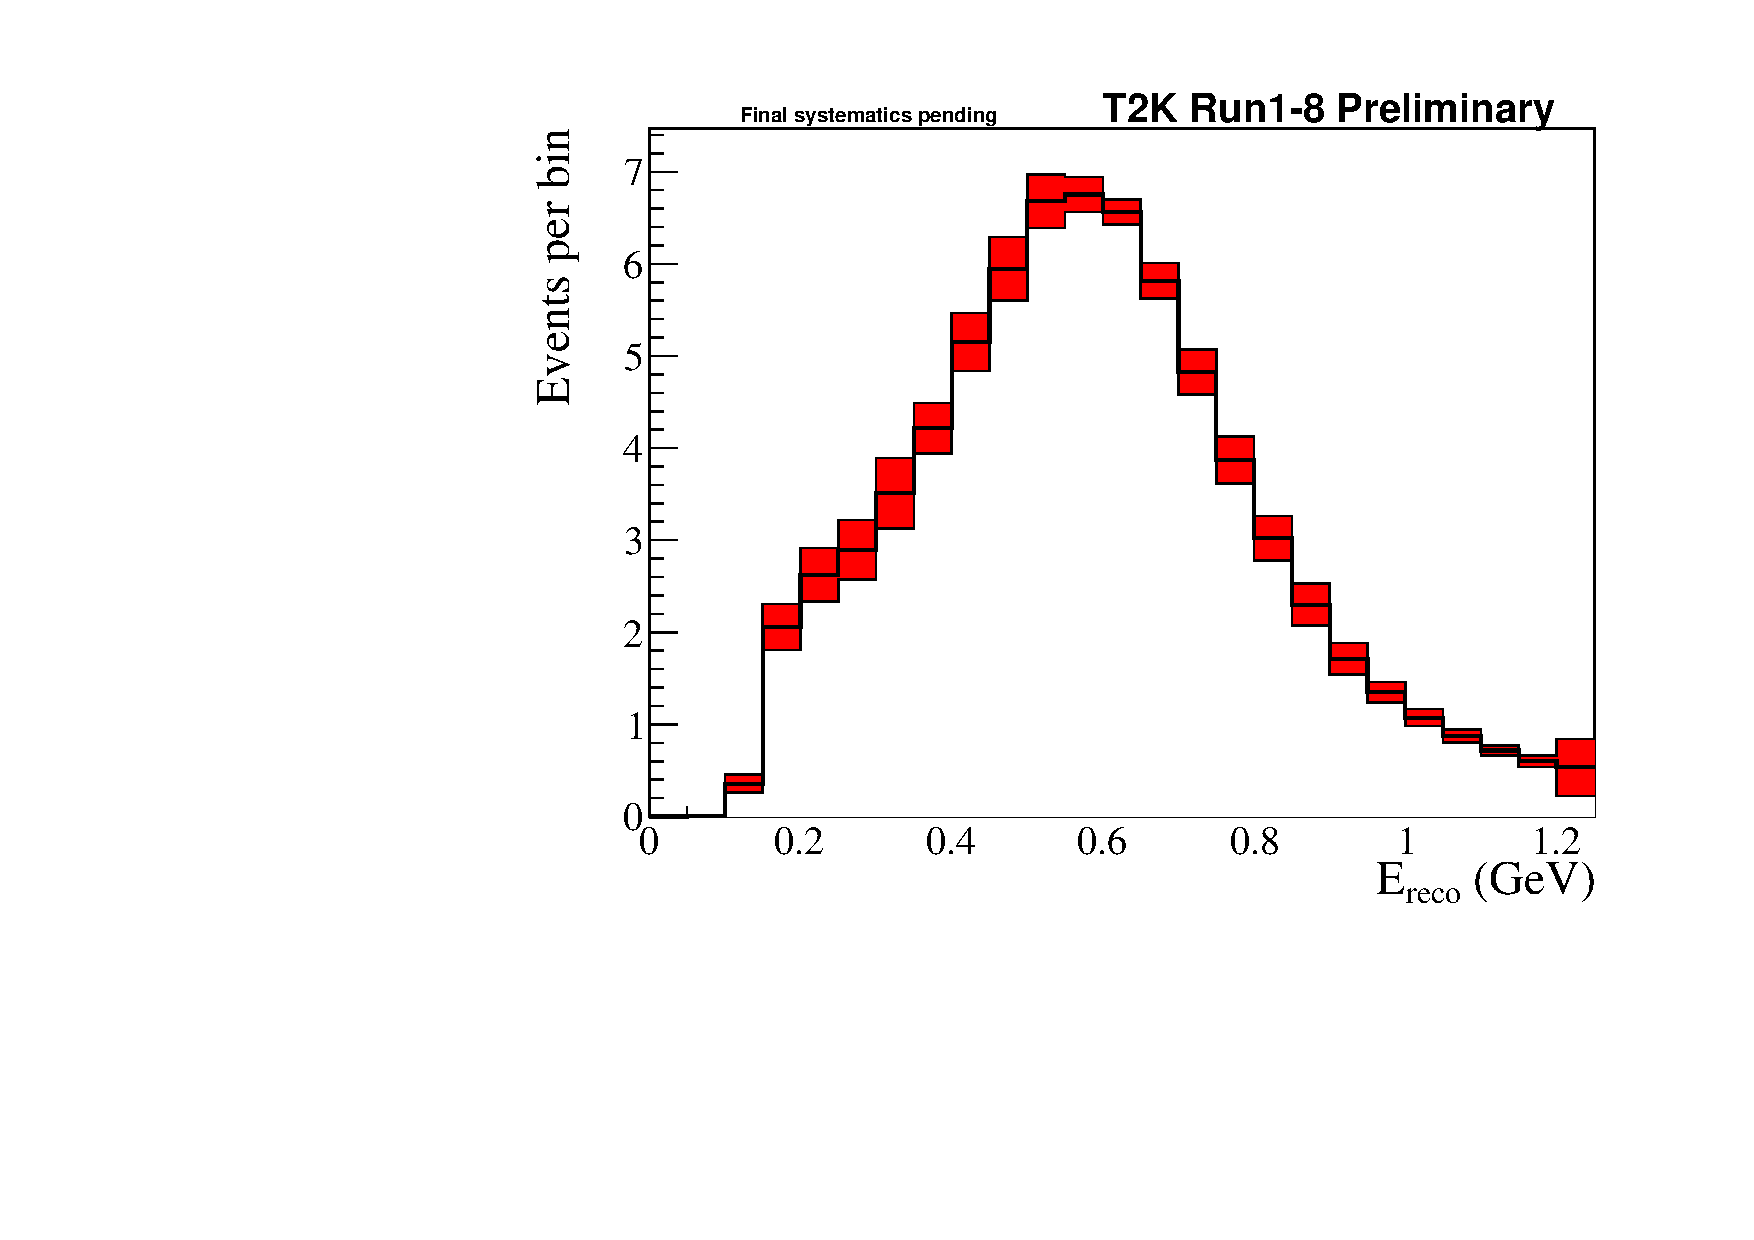
\includegraphics[width=0.9\textwidth]{systematics/envelopes/sk_errors/sk_error_table_1Re_skfsi_envelope}
		\caption{Electron-like, neutrino mode}
	\end{subfigure}
	\begin{subfigure}[b]{0.49\textwidth}
		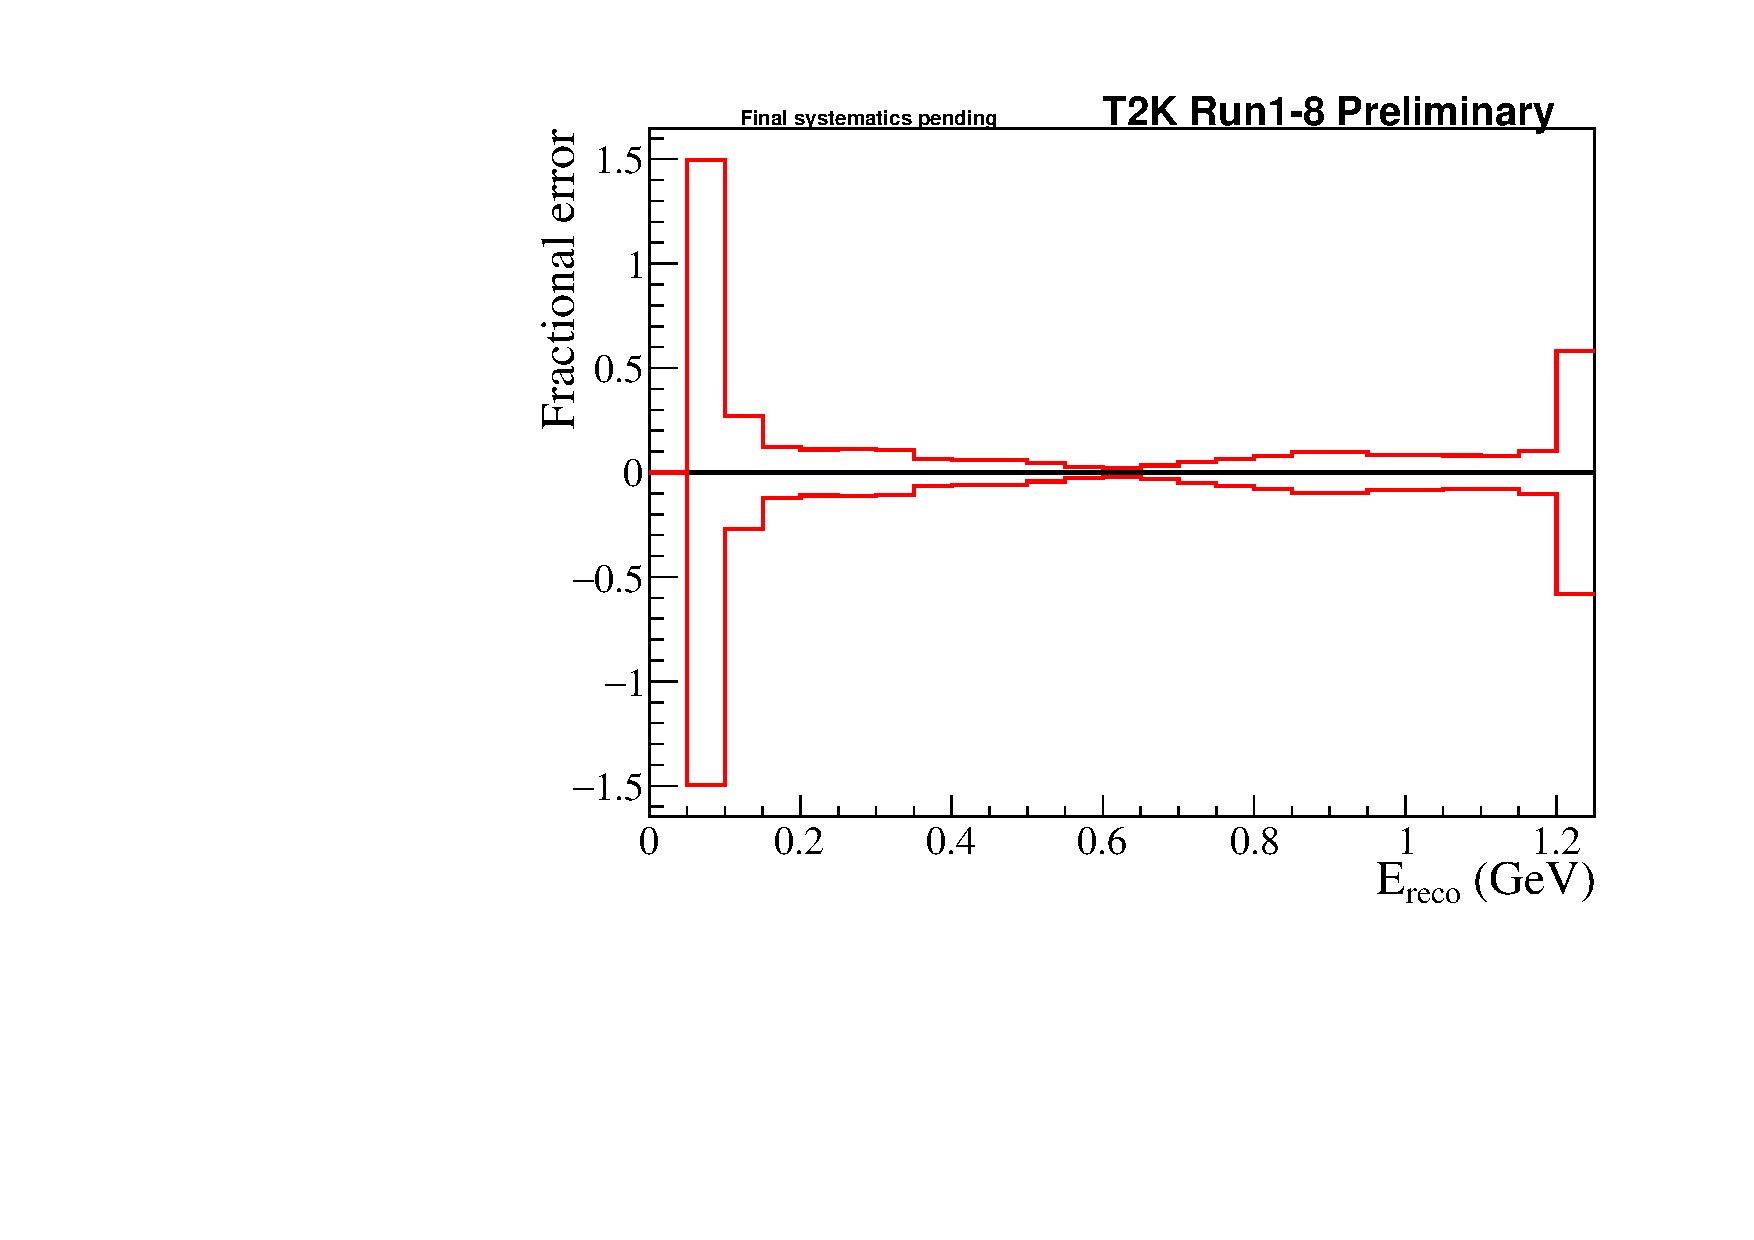
\includegraphics[width=0.9\textwidth]{systematics/envelopes/sk_errors/sk_error_table_1Re_skfsi_envelope_fractional}
		\caption{Electron-like, neutrino mode}
	\end{subfigure}
	\begin{subfigure}[b]{0.49\textwidth}
		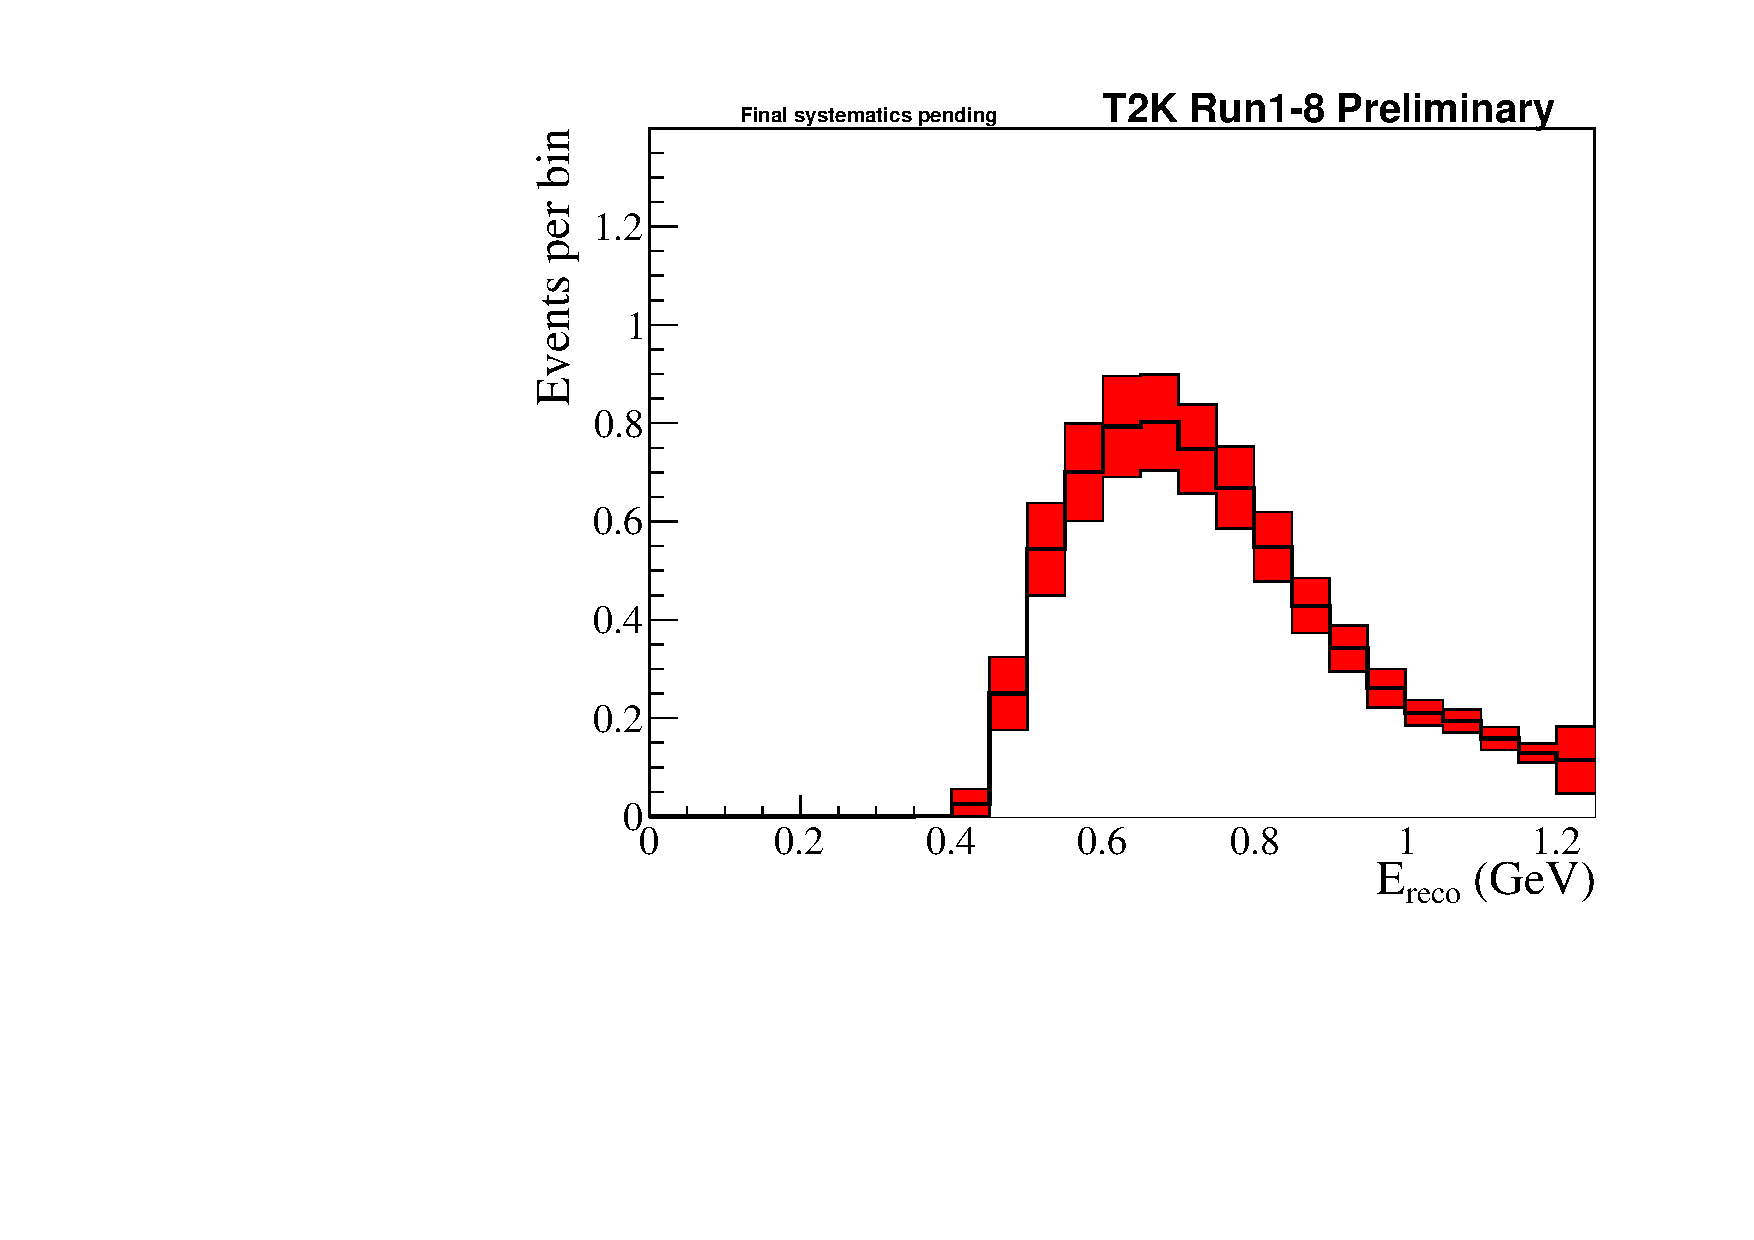
\includegraphics[width=0.9\textwidth]{systematics/envelopes/sk_errors/sk_error_table_MultiRe_skfsi_envelope}
		\caption{\nueCConepi-like, neutrino mode}
	\end{subfigure}
	\begin{subfigure}[b]{0.49\textwidth}
		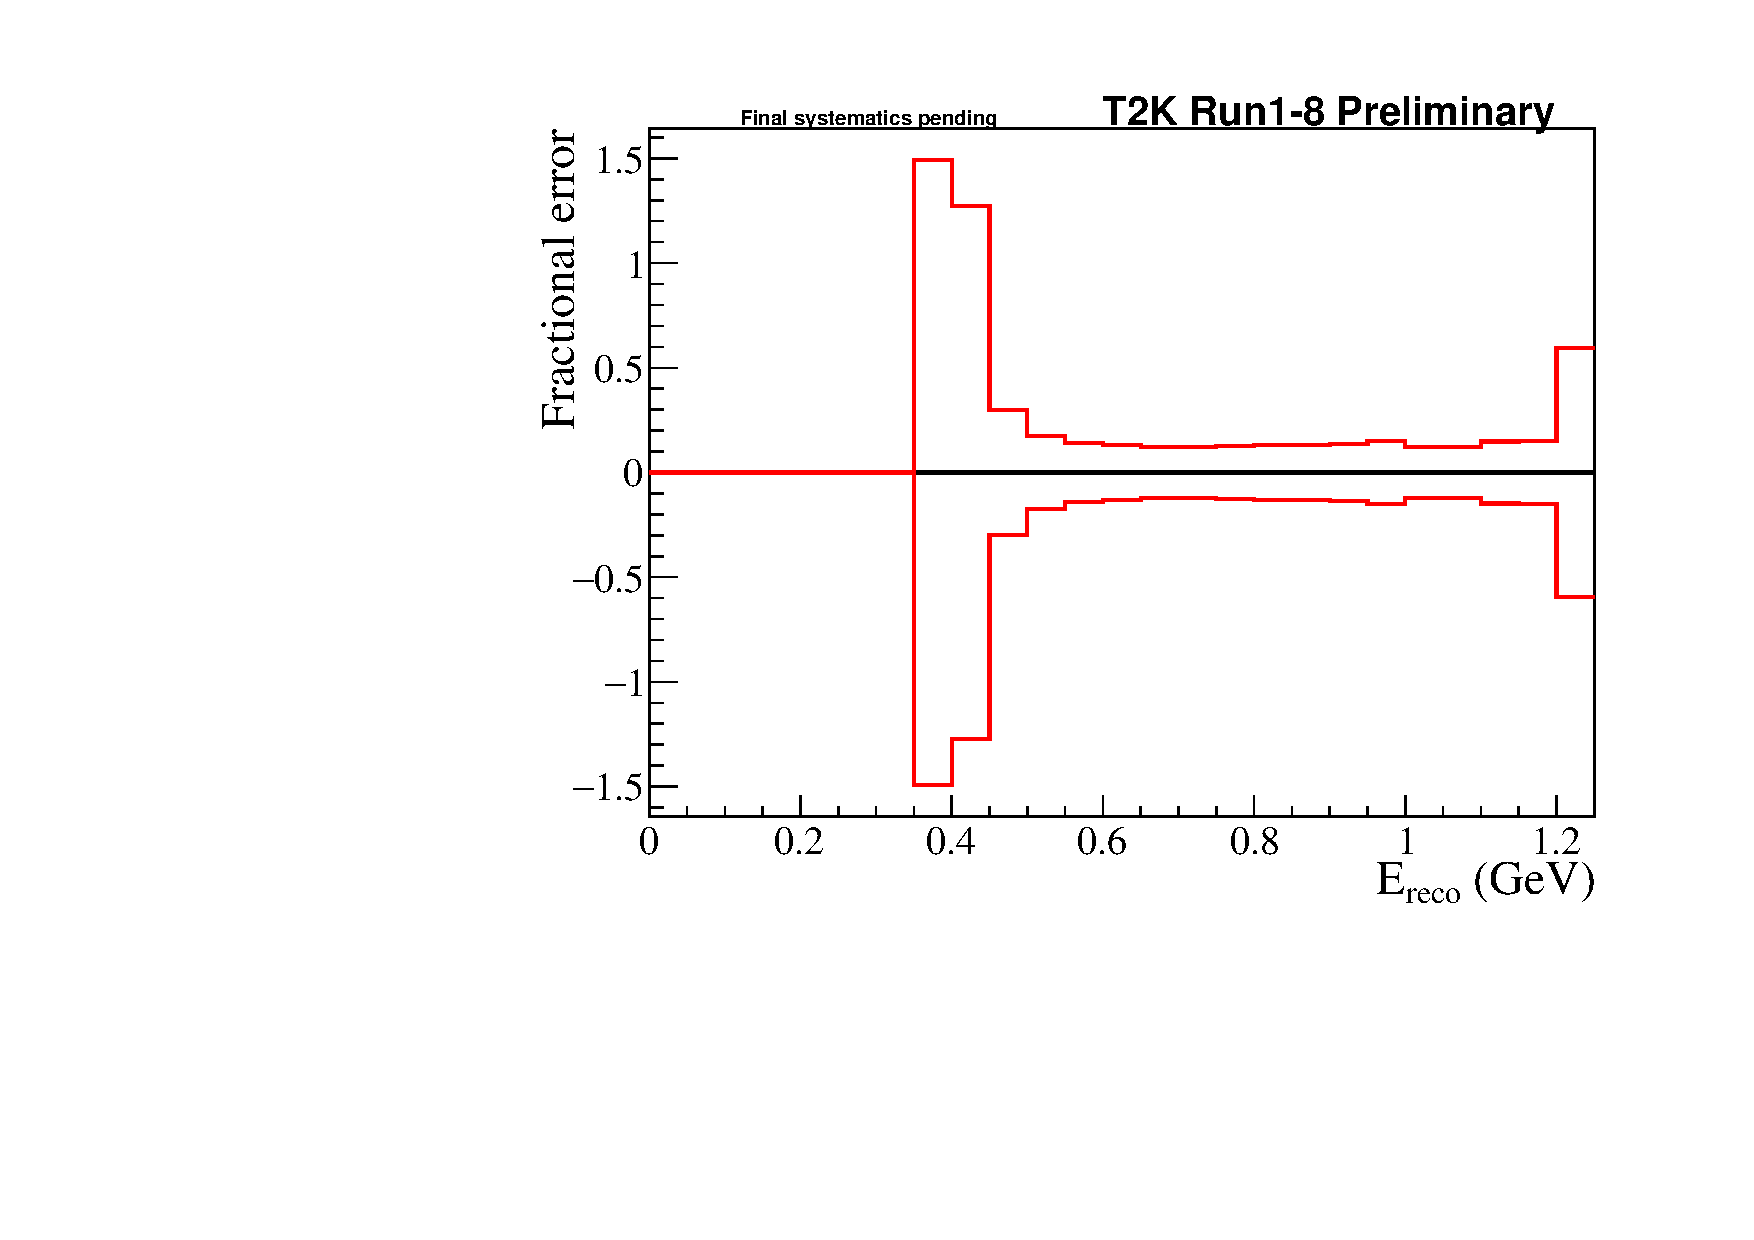
\includegraphics[width=0.9\textwidth]{systematics/envelopes/sk_errors/sk_error_table_MultiRe_skfsi_envelope_fractional}
		\caption{\nueCConepi-like, neutrino mode}
	\end{subfigure}
	\caption {
		Error envelopes (left) and fractional error (right) for the reconstructed neutrino energy spectrum for Super-K FSI+SI+PN systematic parameters. \num{1e4} toys are generated for the Asimov data set A with randomized systematic parameters with correlations taken into account.
	}
	\label{fig:sk_envelopes_skfsi}
\end{figure*}
\clearpage

\begin{figure*}
	\center
	\begin{subfigure}[b]{0.49\textwidth}
		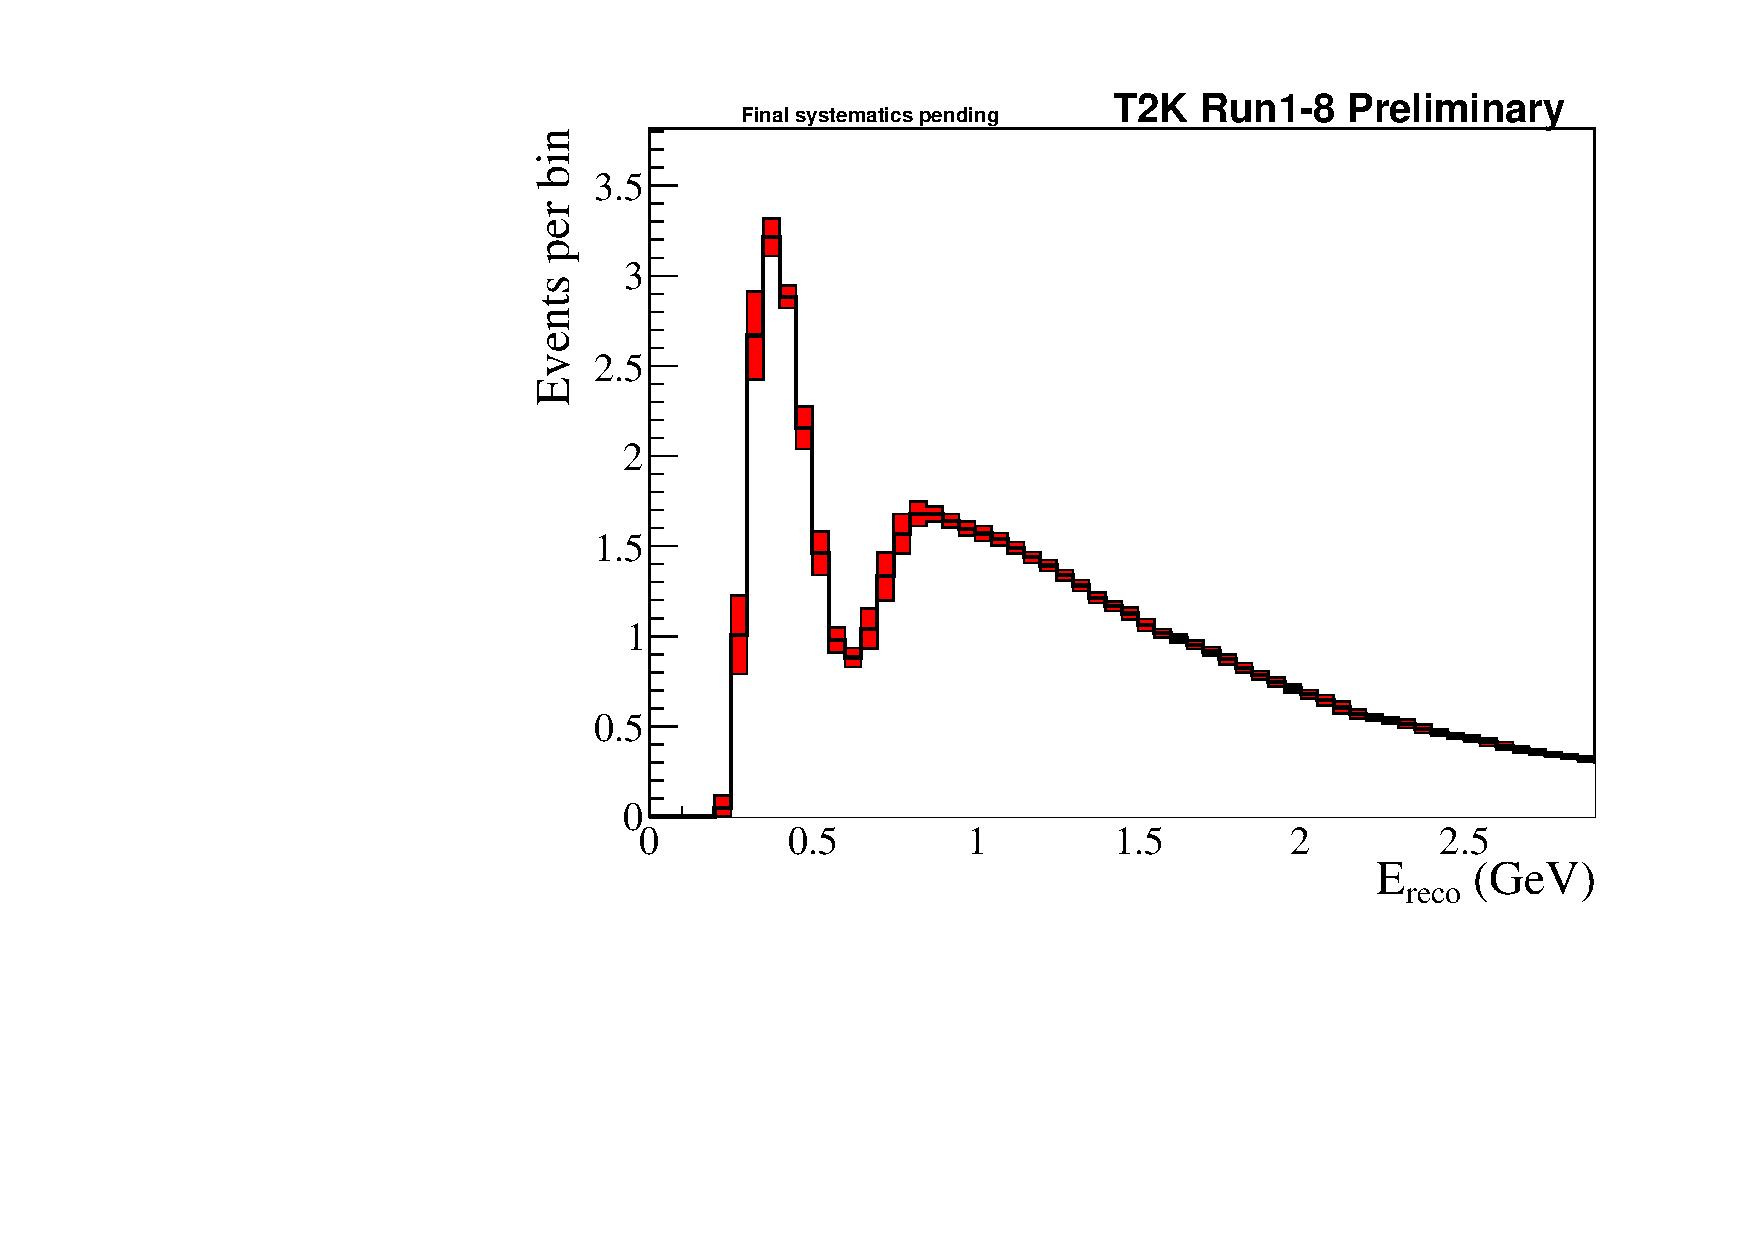
\includegraphics[width=0.9\textwidth]{systematics/envelopes/sk_errors/sk_error_table_RHC1Rmu_skfsi_envelope}
		\caption{Muon-like, antineutrino mode}
	\end{subfigure}
	\begin{subfigure}[b]{0.49\textwidth}
		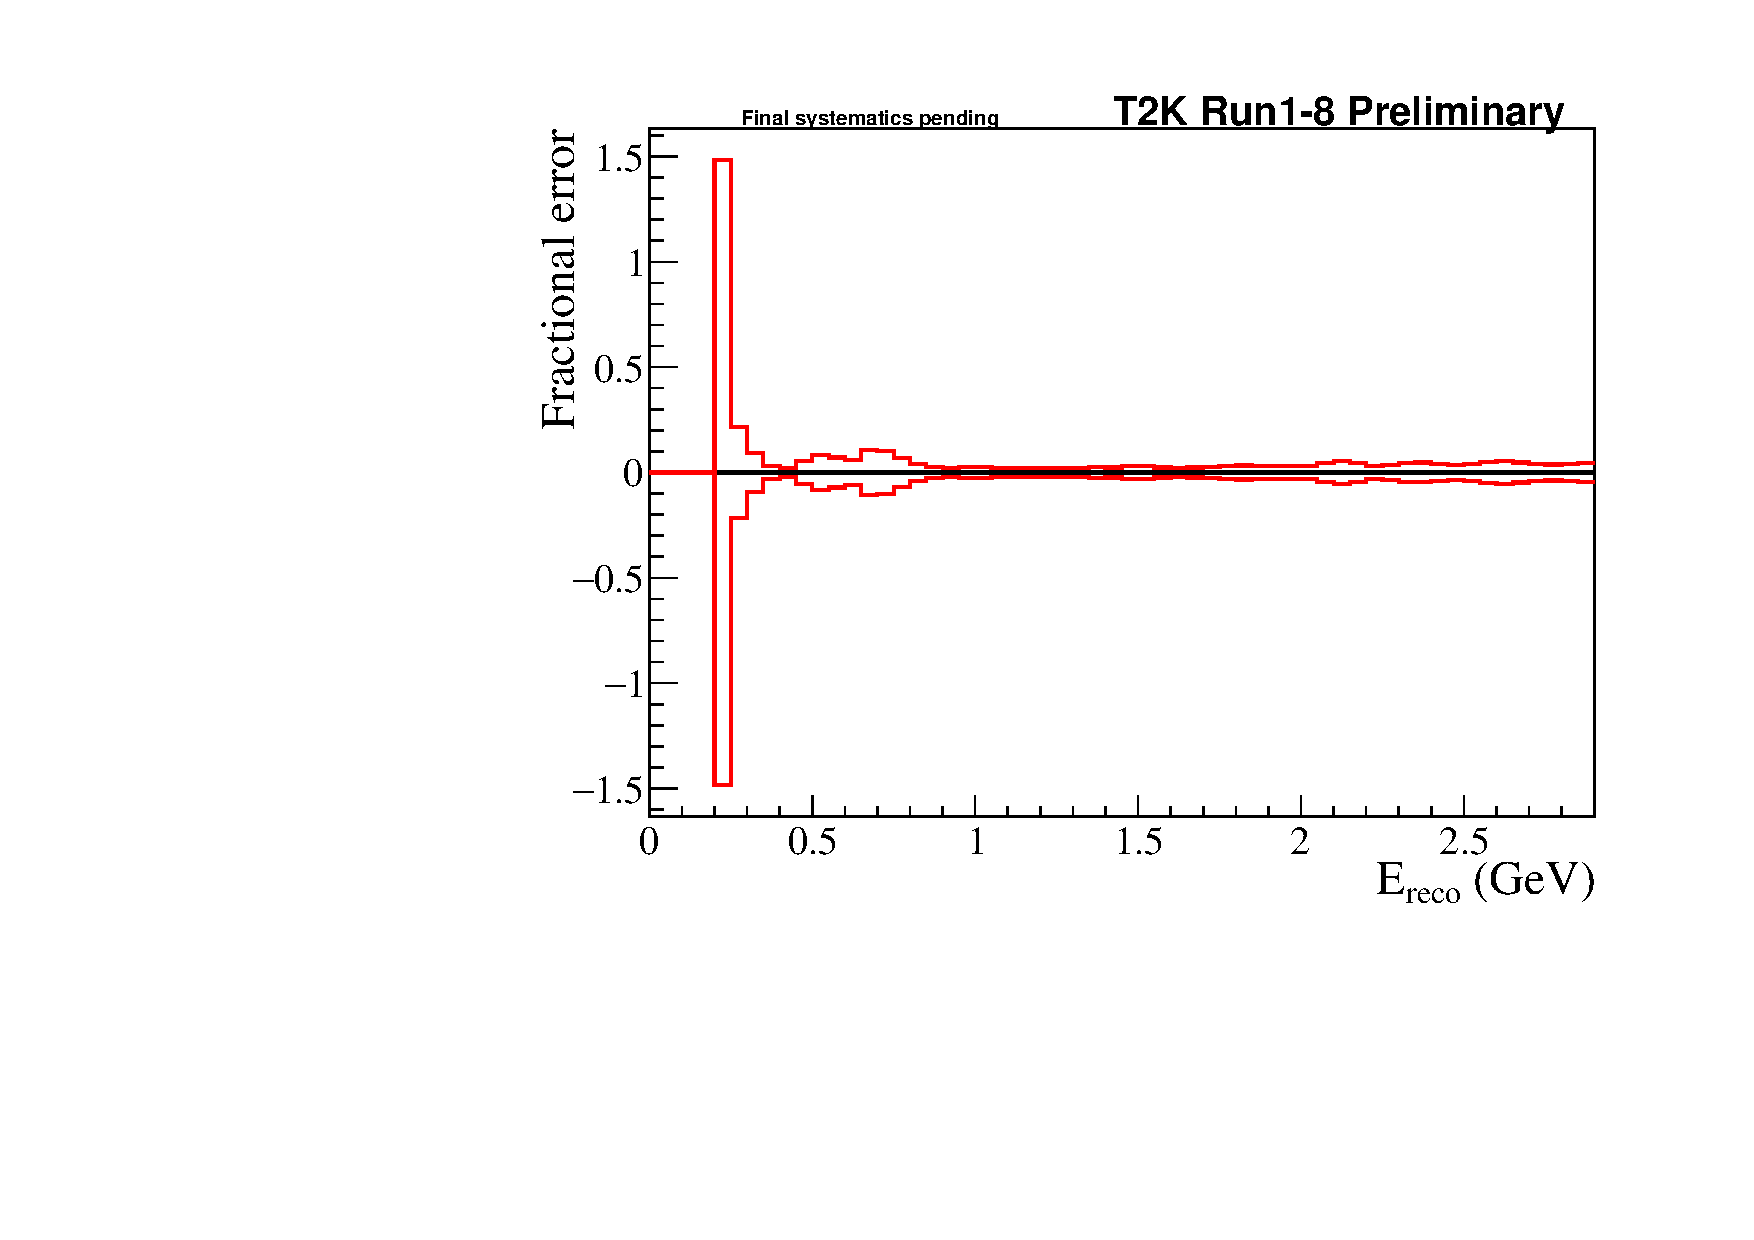
\includegraphics[width=0.9\textwidth]{systematics/envelopes/sk_errors/sk_error_table_RHC1Rmu_skfsi_envelope_fractional}
		\caption{Muon-like, antineutrino mode}
	\end{subfigure}
	\begin{subfigure}[b]{0.49\textwidth}
		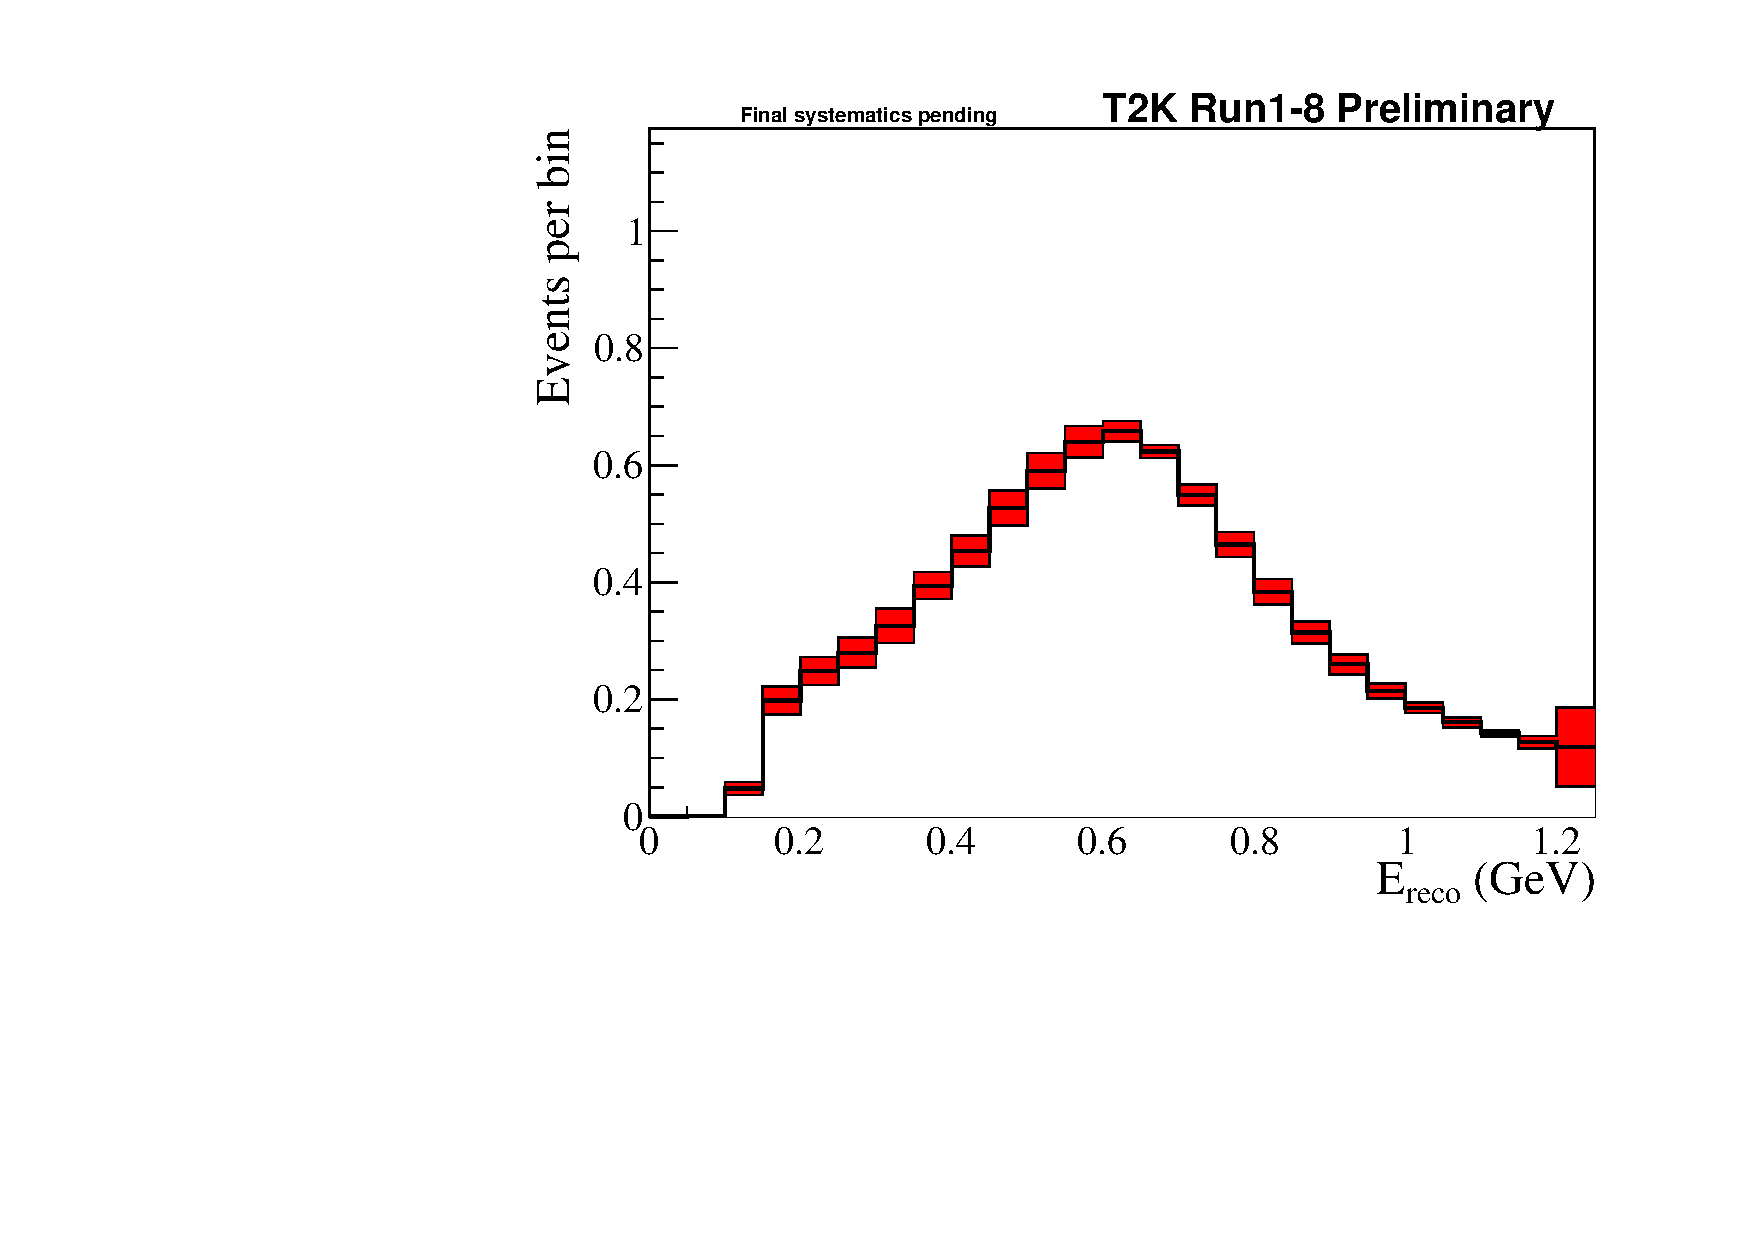
\includegraphics[width=0.9\textwidth]{systematics/envelopes/sk_errors/sk_error_table_RHC1Re_skfsi_envelope}
		\caption{Electron-like antineutrino mode}
	\end{subfigure}
	\begin{subfigure}[b]{0.49\textwidth}
		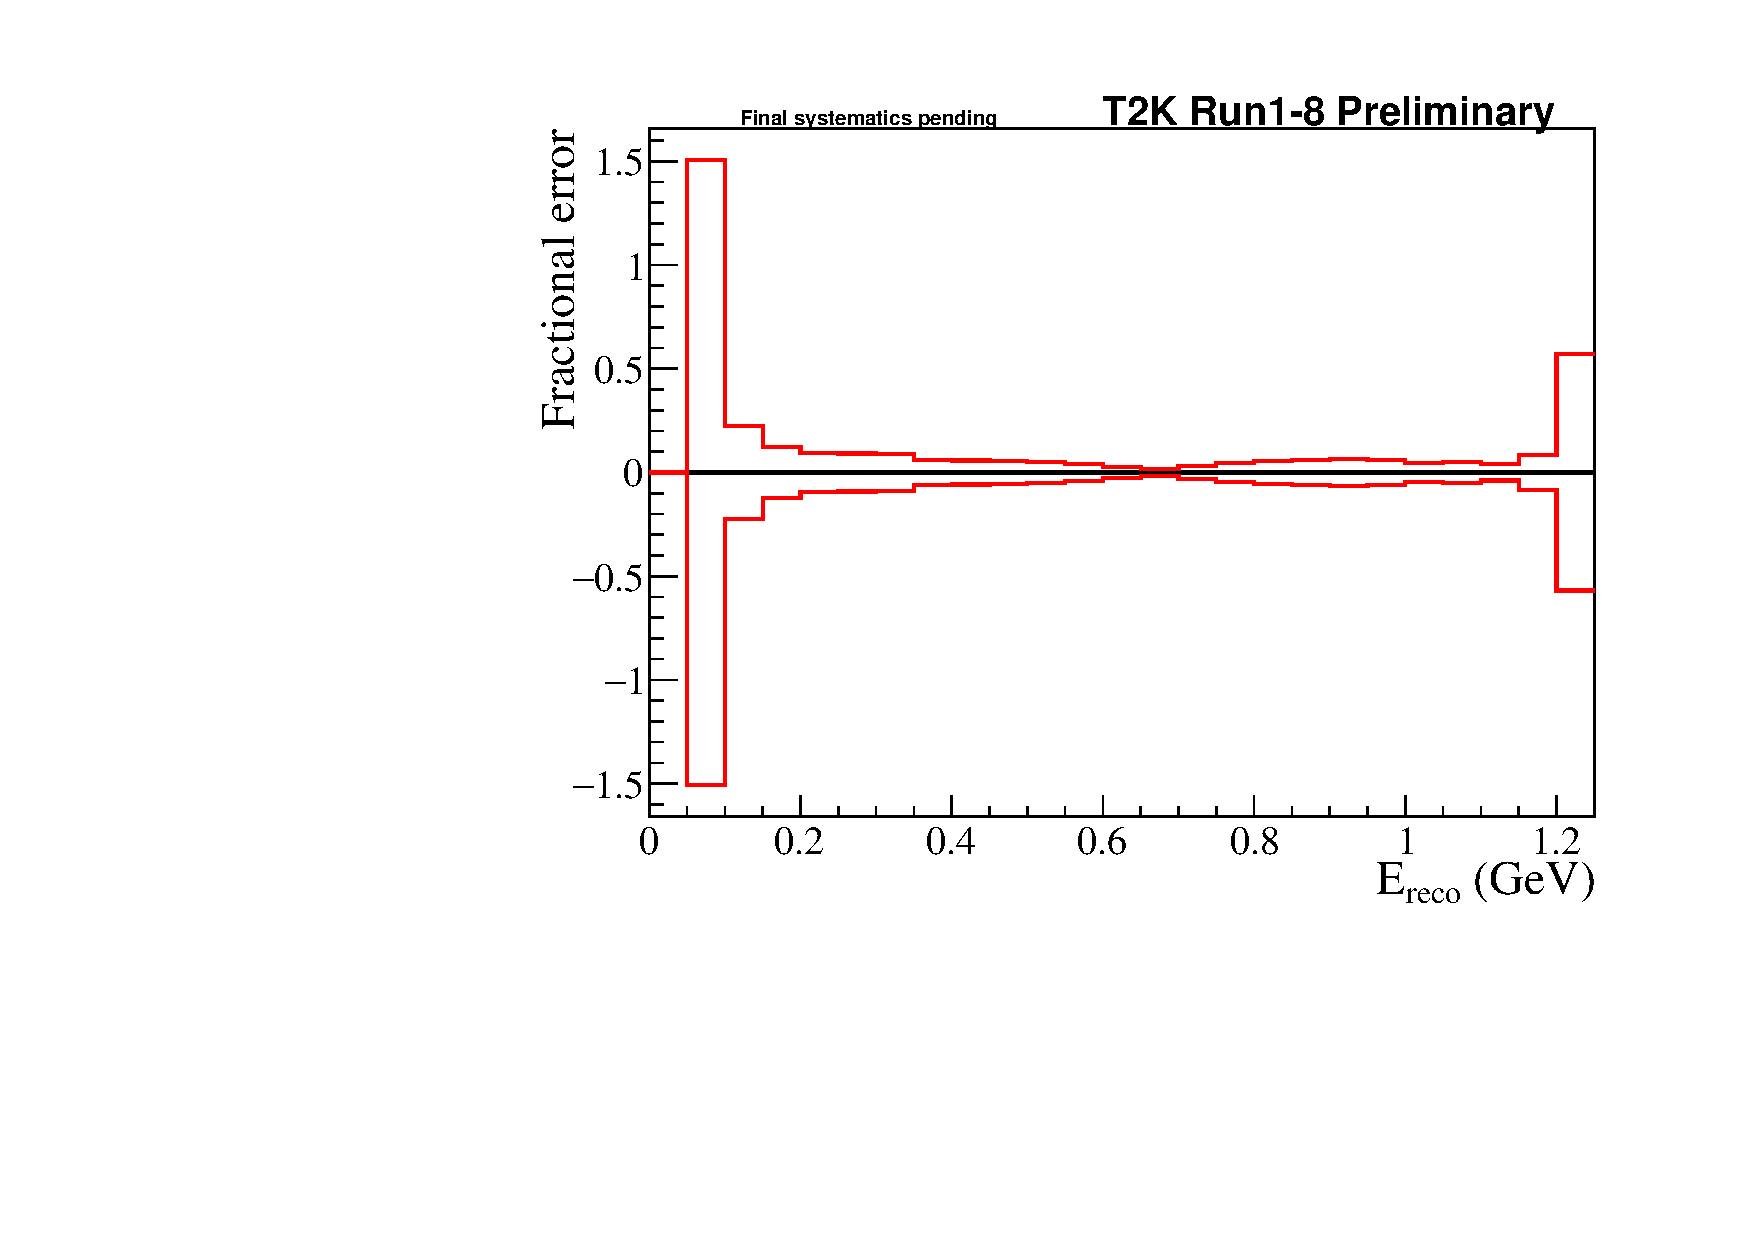
\includegraphics[width=0.9\textwidth]{systematics/envelopes/sk_errors/sk_error_table_RHC1Re_skfsi_envelope_fractional}
		\caption{Electron-like antineutrino mode}
	\end{subfigure}
	\caption {
		Error envelopes (left) and fractional errors (right) for the reconstructed neutrino energy spectrum for Super-K FSI+SI+PN systematic parameters. \num{1e4} toys are generated for the Asimov data set A with randomized systematic parameters with correlations taken into account.
	}
	\label{fig:sk_envelopes_skfsi_b}
\end{figure*}
\clearpage
\begin{figure*}
	\center
	\begin{subfigure}[b]{0.49\textwidth}
		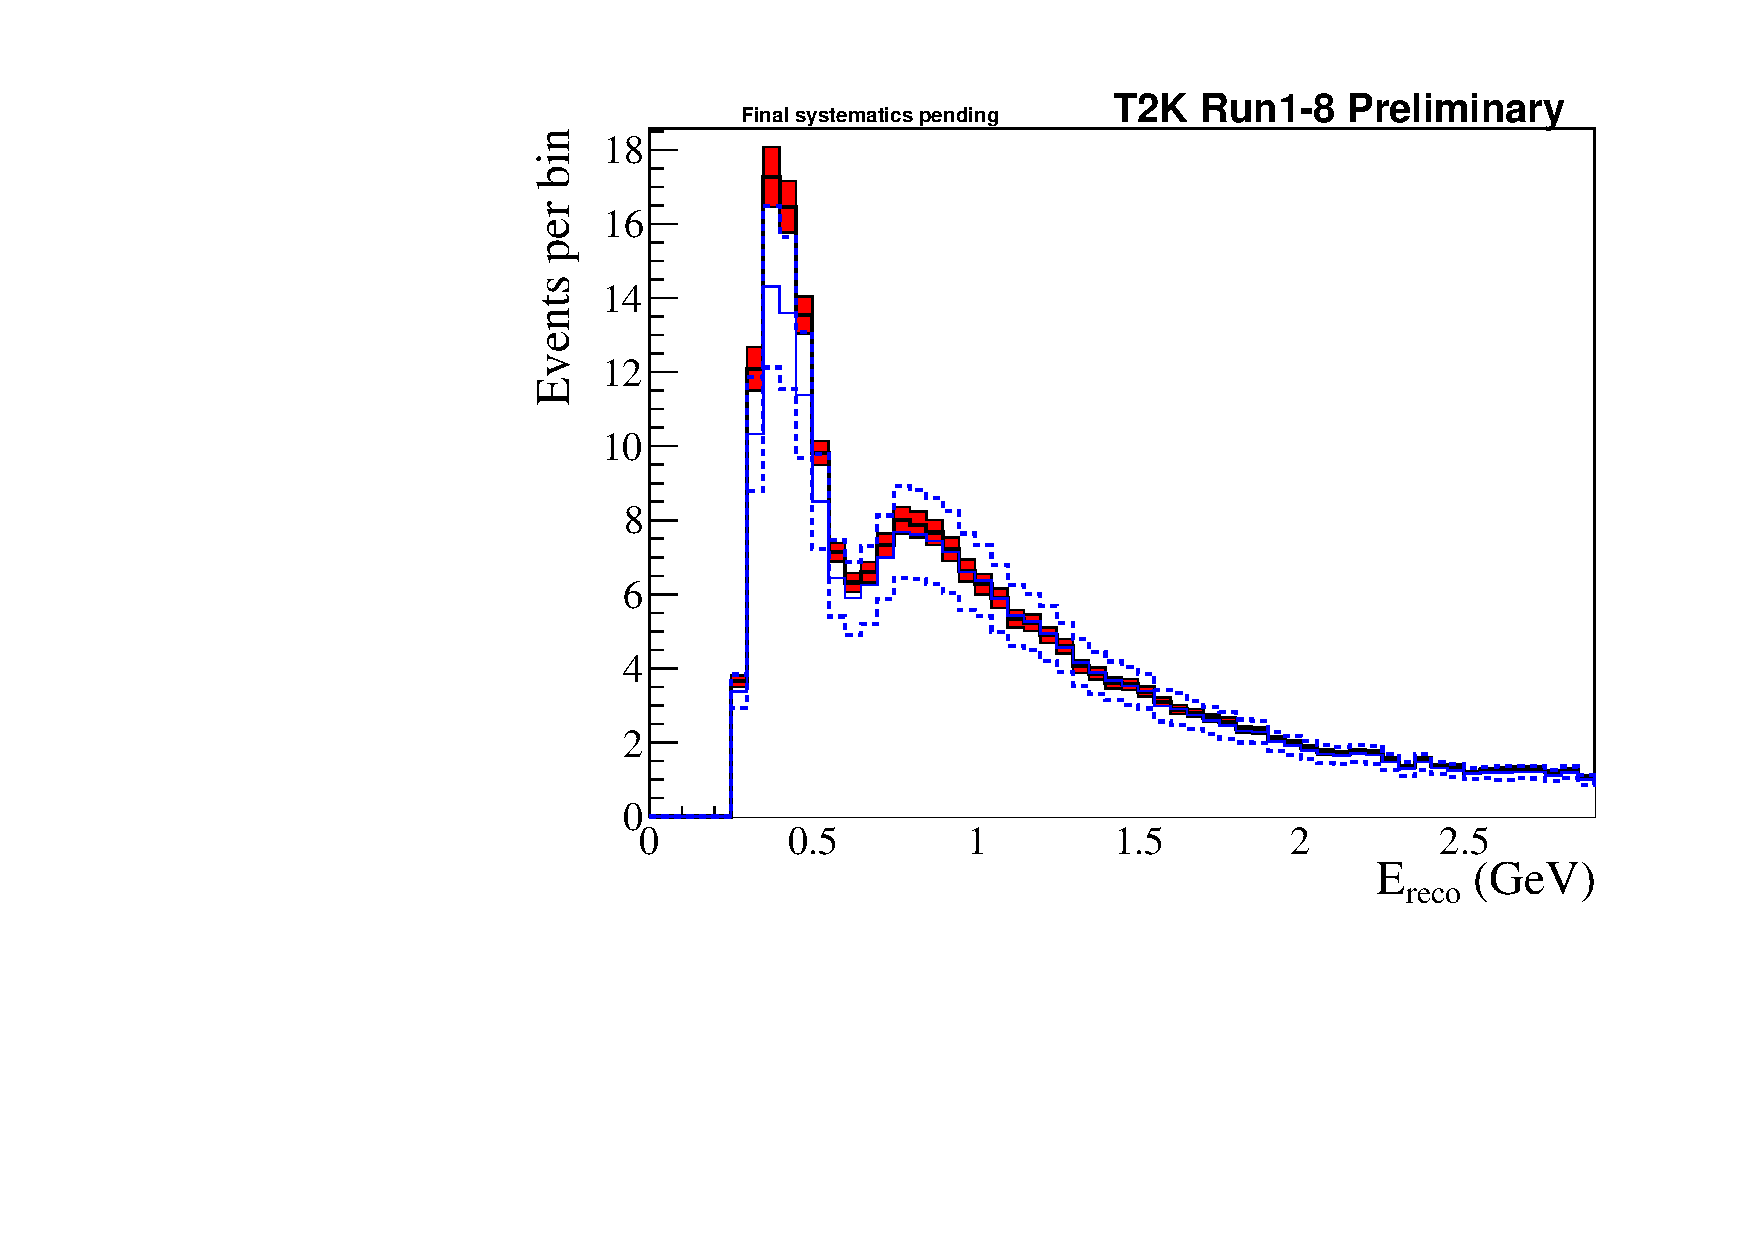
\includegraphics[width=0.9\textwidth]{systematics/envelopes/sk_errors/sk_error_table_1Rmu_banff_constrained_envelope}
		\caption{Muon-like, neutrino mode}
	\end{subfigure}
	\begin{subfigure}[b]{0.49\textwidth}
		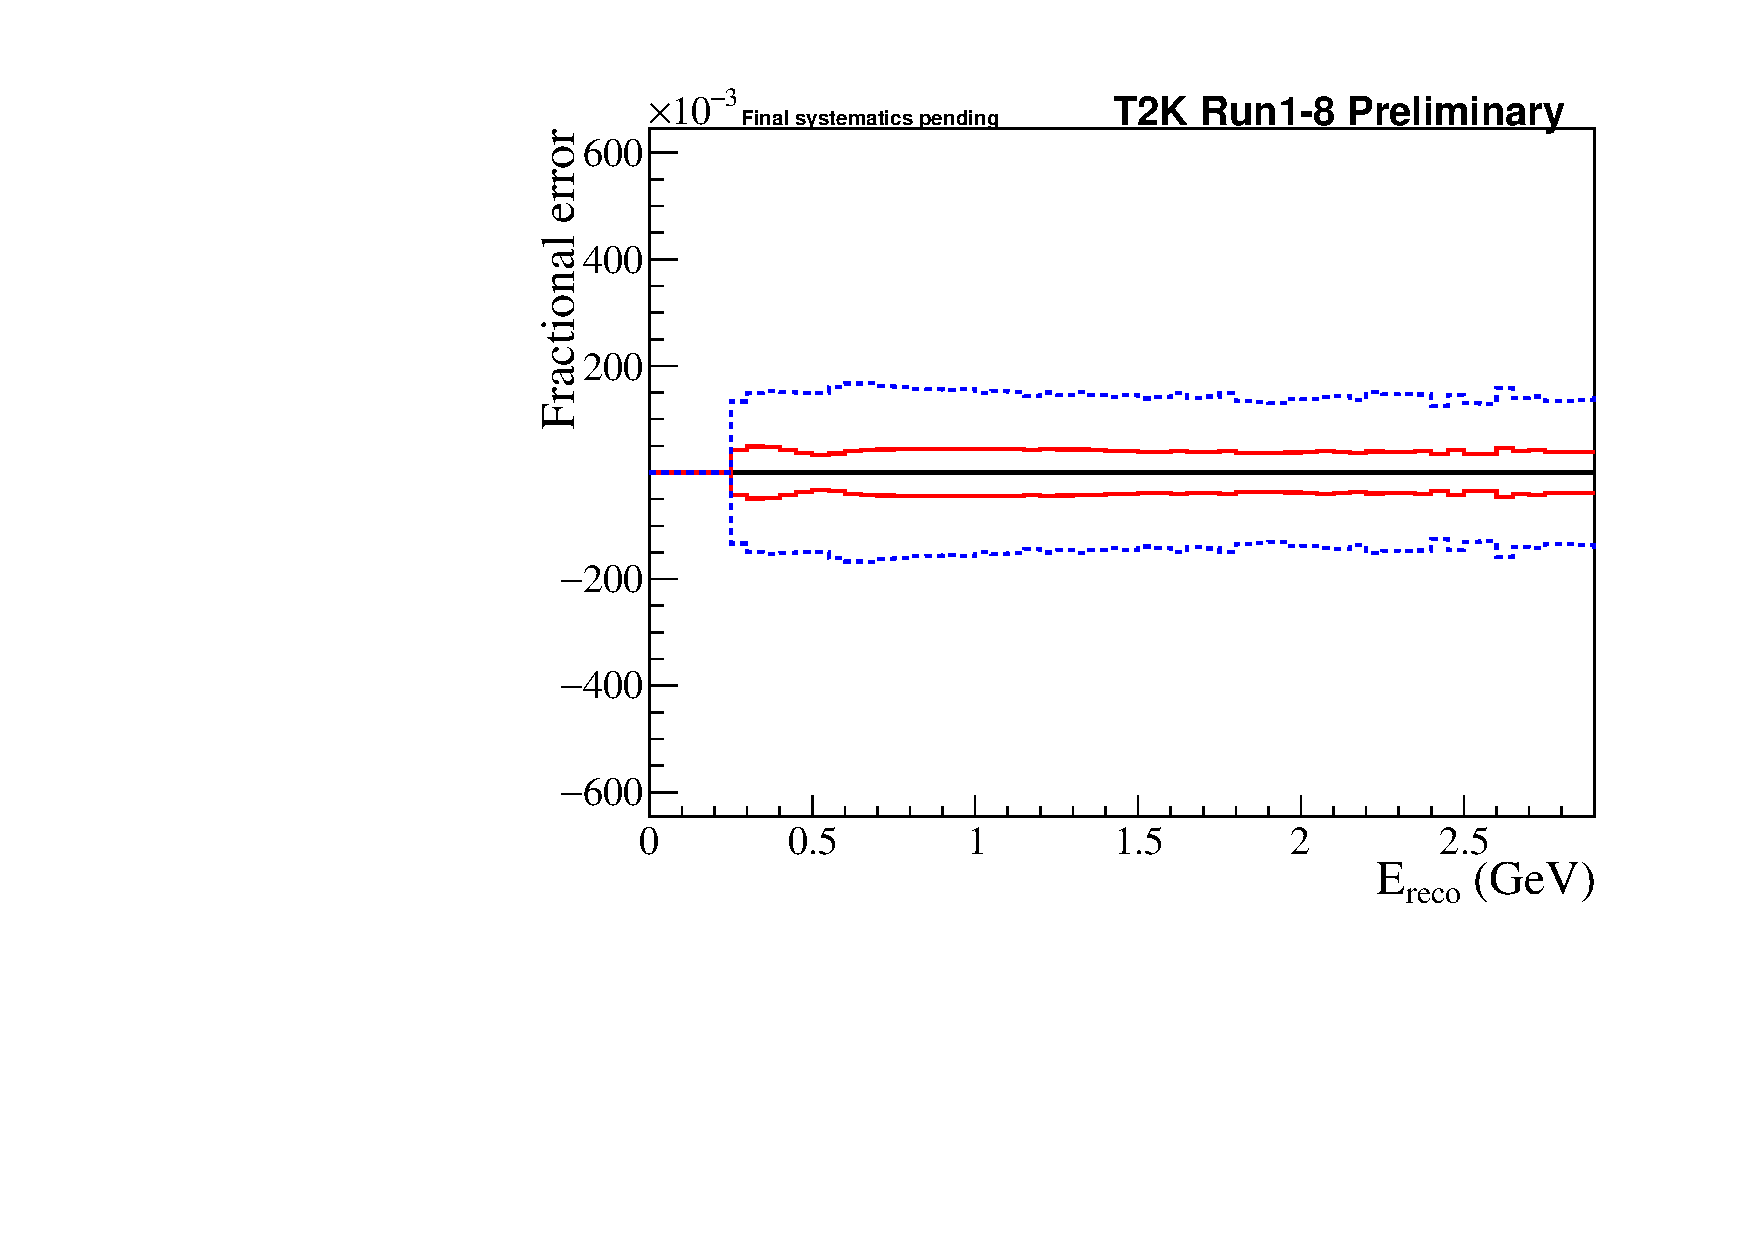
\includegraphics[width=0.9\textwidth]{systematics/envelopes/sk_errors/sk_error_table_1Rmu_banff_constrained_envelope_fractional}
		\caption{Muon-like, neutrino mode}
	\end{subfigure}
	\begin{subfigure}[b]{0.49\textwidth}
		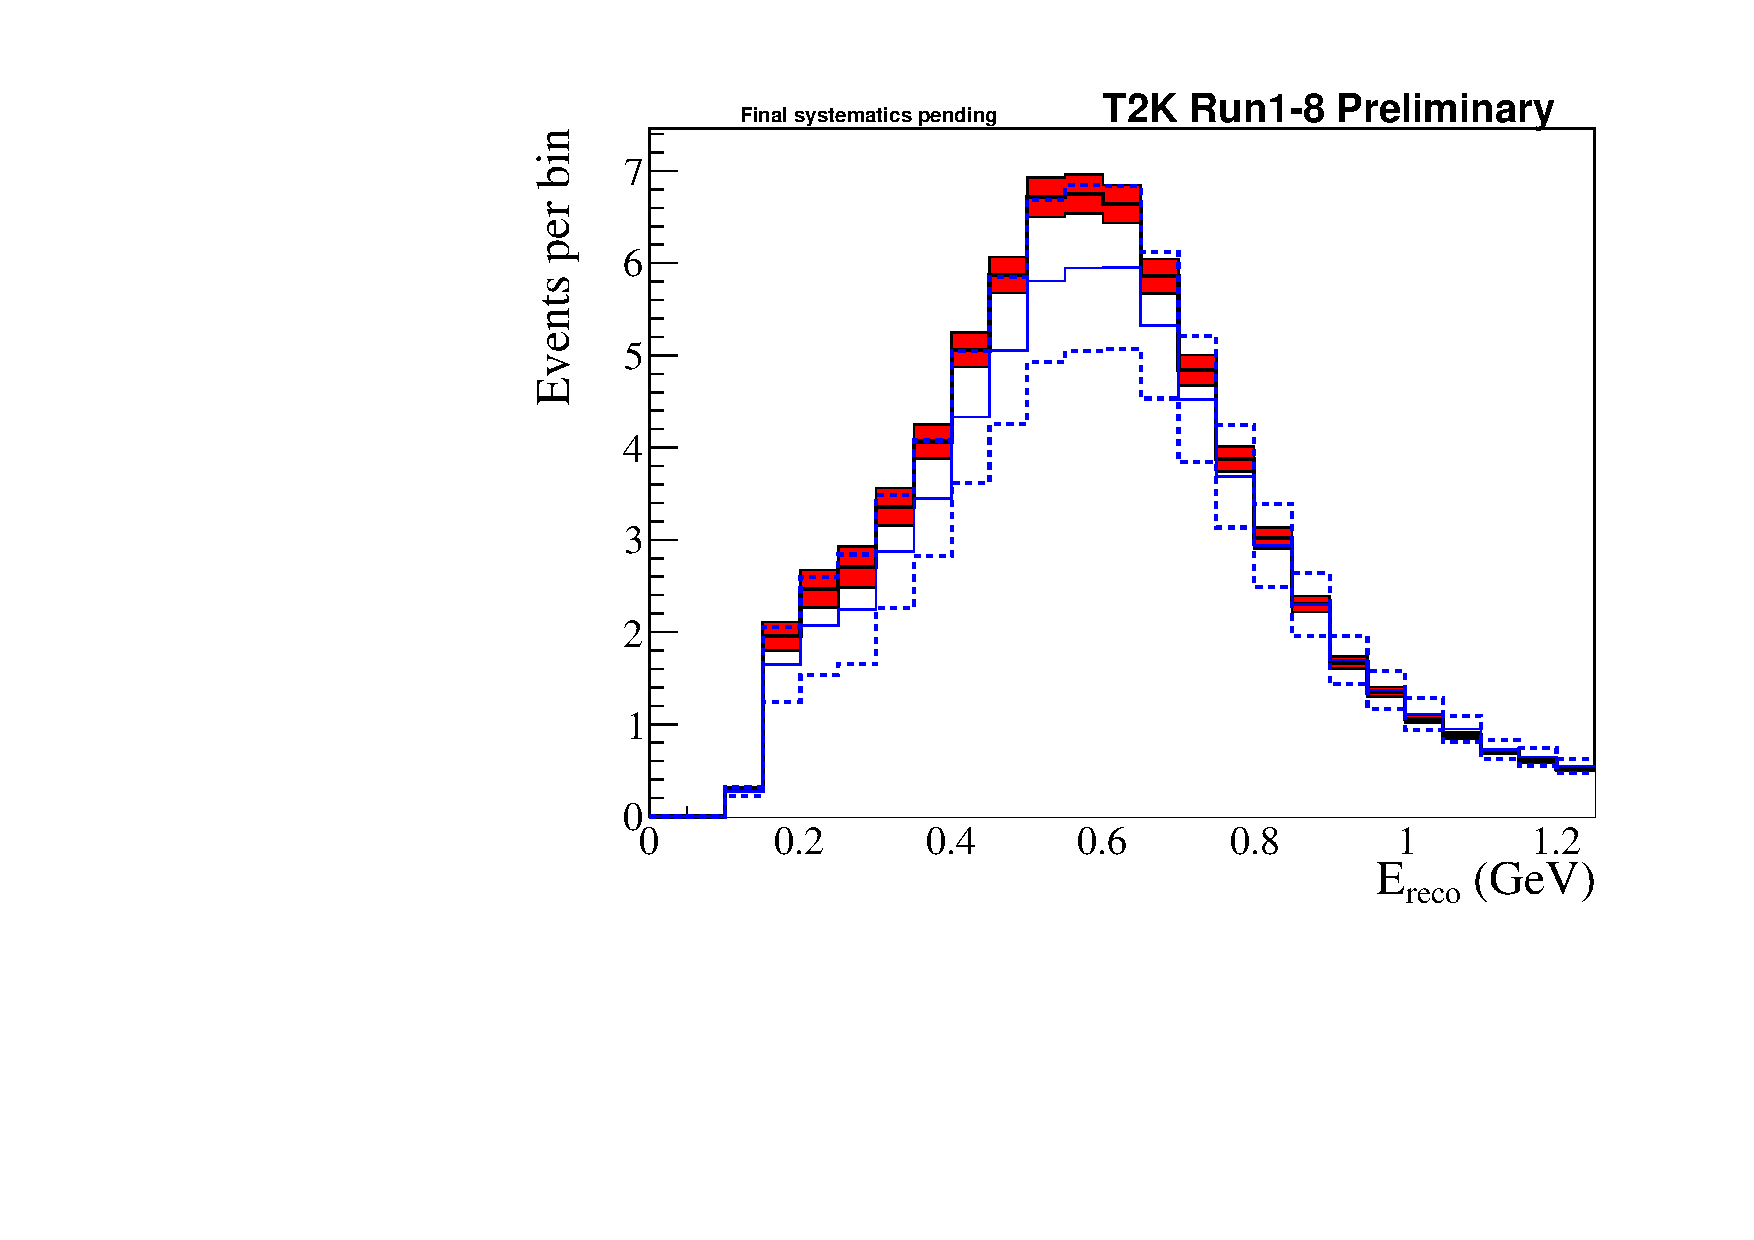
\includegraphics[width=0.9\textwidth]{systematics/envelopes/sk_errors/sk_error_table_1Re_banff_constrained_envelope}
		\caption{Electron-like, neutrino mode}
	\end{subfigure}
	\begin{subfigure}[b]{0.49\textwidth}
		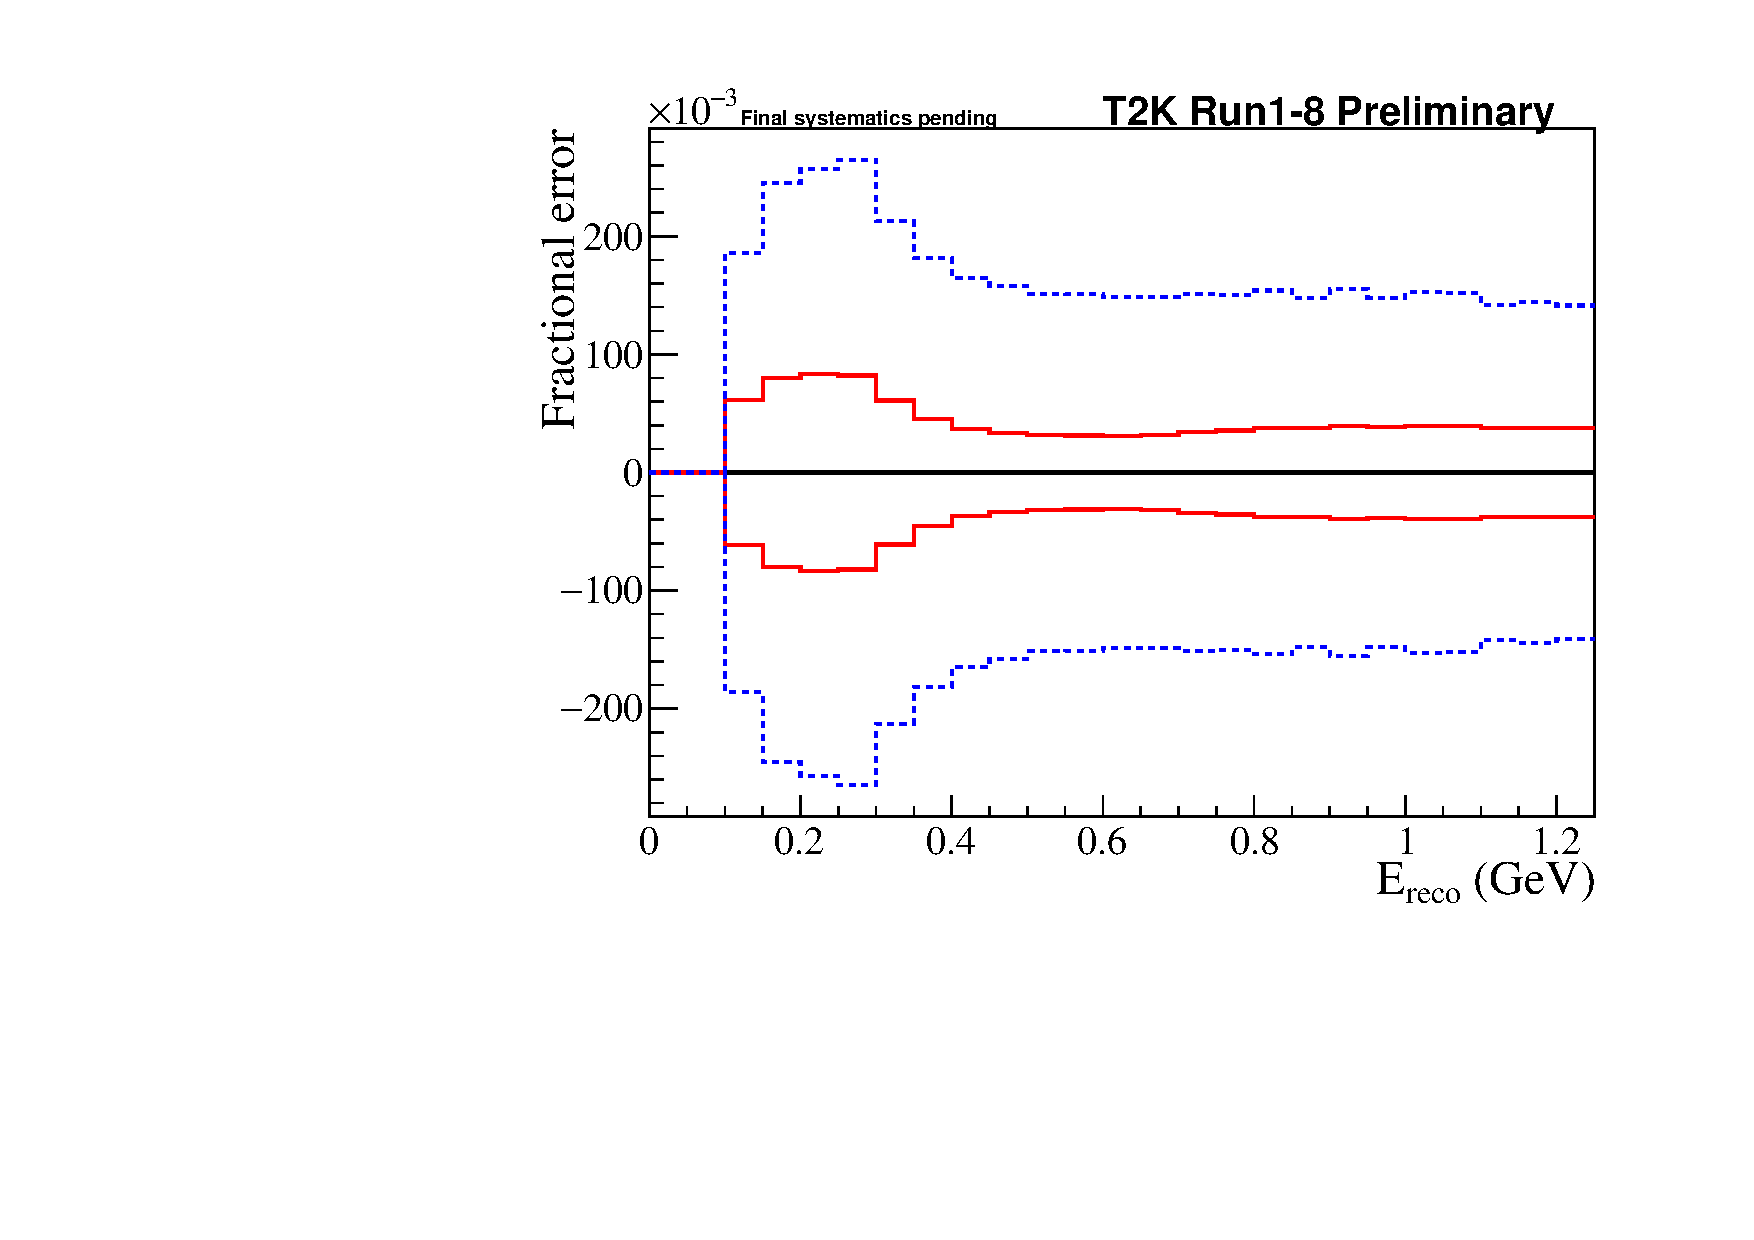
\includegraphics[width=0.9\textwidth]{systematics/envelopes/sk_errors/sk_error_table_1Re_banff_constrained_envelope_fractional}
		\caption{Electron-like, neutrino mode}
	\end{subfigure}
	\begin{subfigure}[b]{0.49\textwidth}
		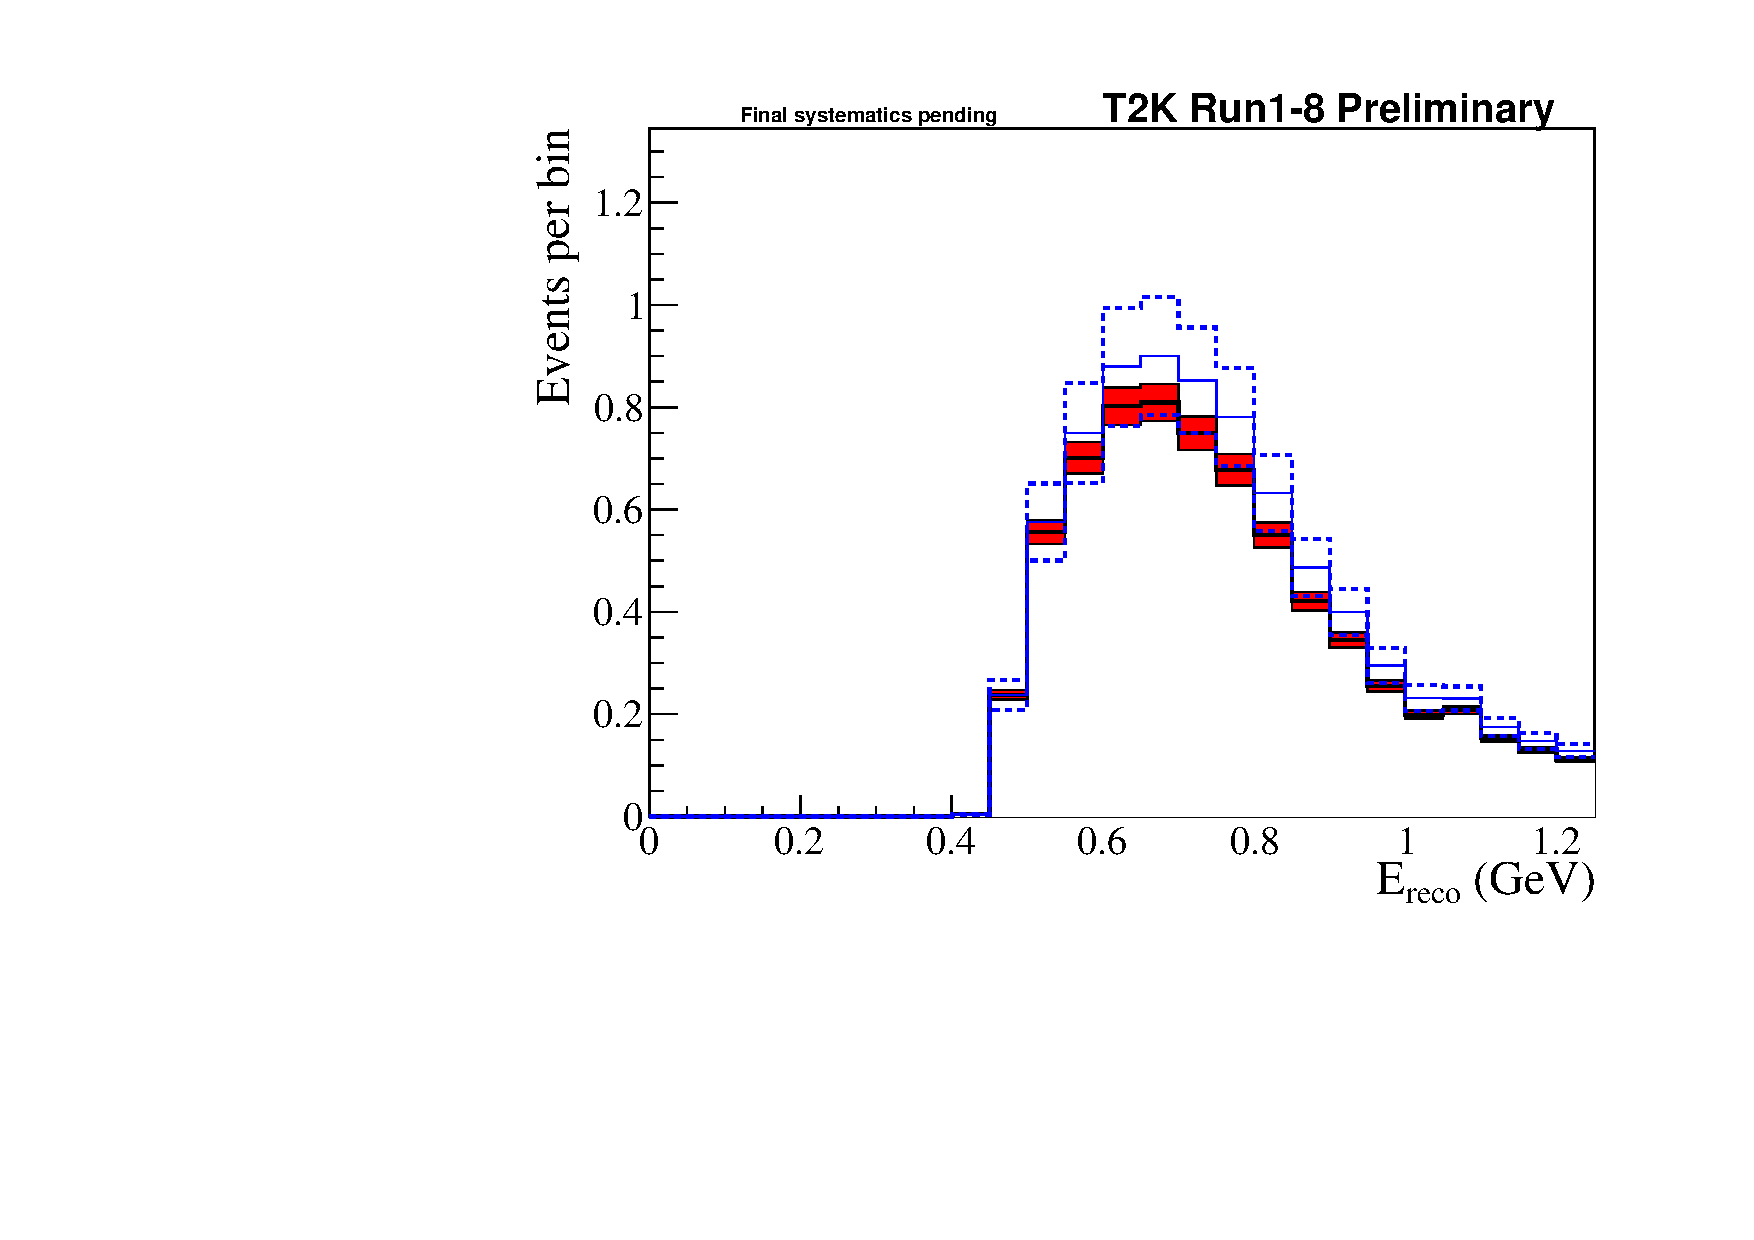
\includegraphics[width=0.9\textwidth]{systematics/envelopes/sk_errors/sk_error_table_MultiRe_banff_constrained_envelope}
		\caption{\nueCConepi-like, neutrino mode}
	\end{subfigure}
	\begin{subfigure}[b]{0.49\textwidth}
		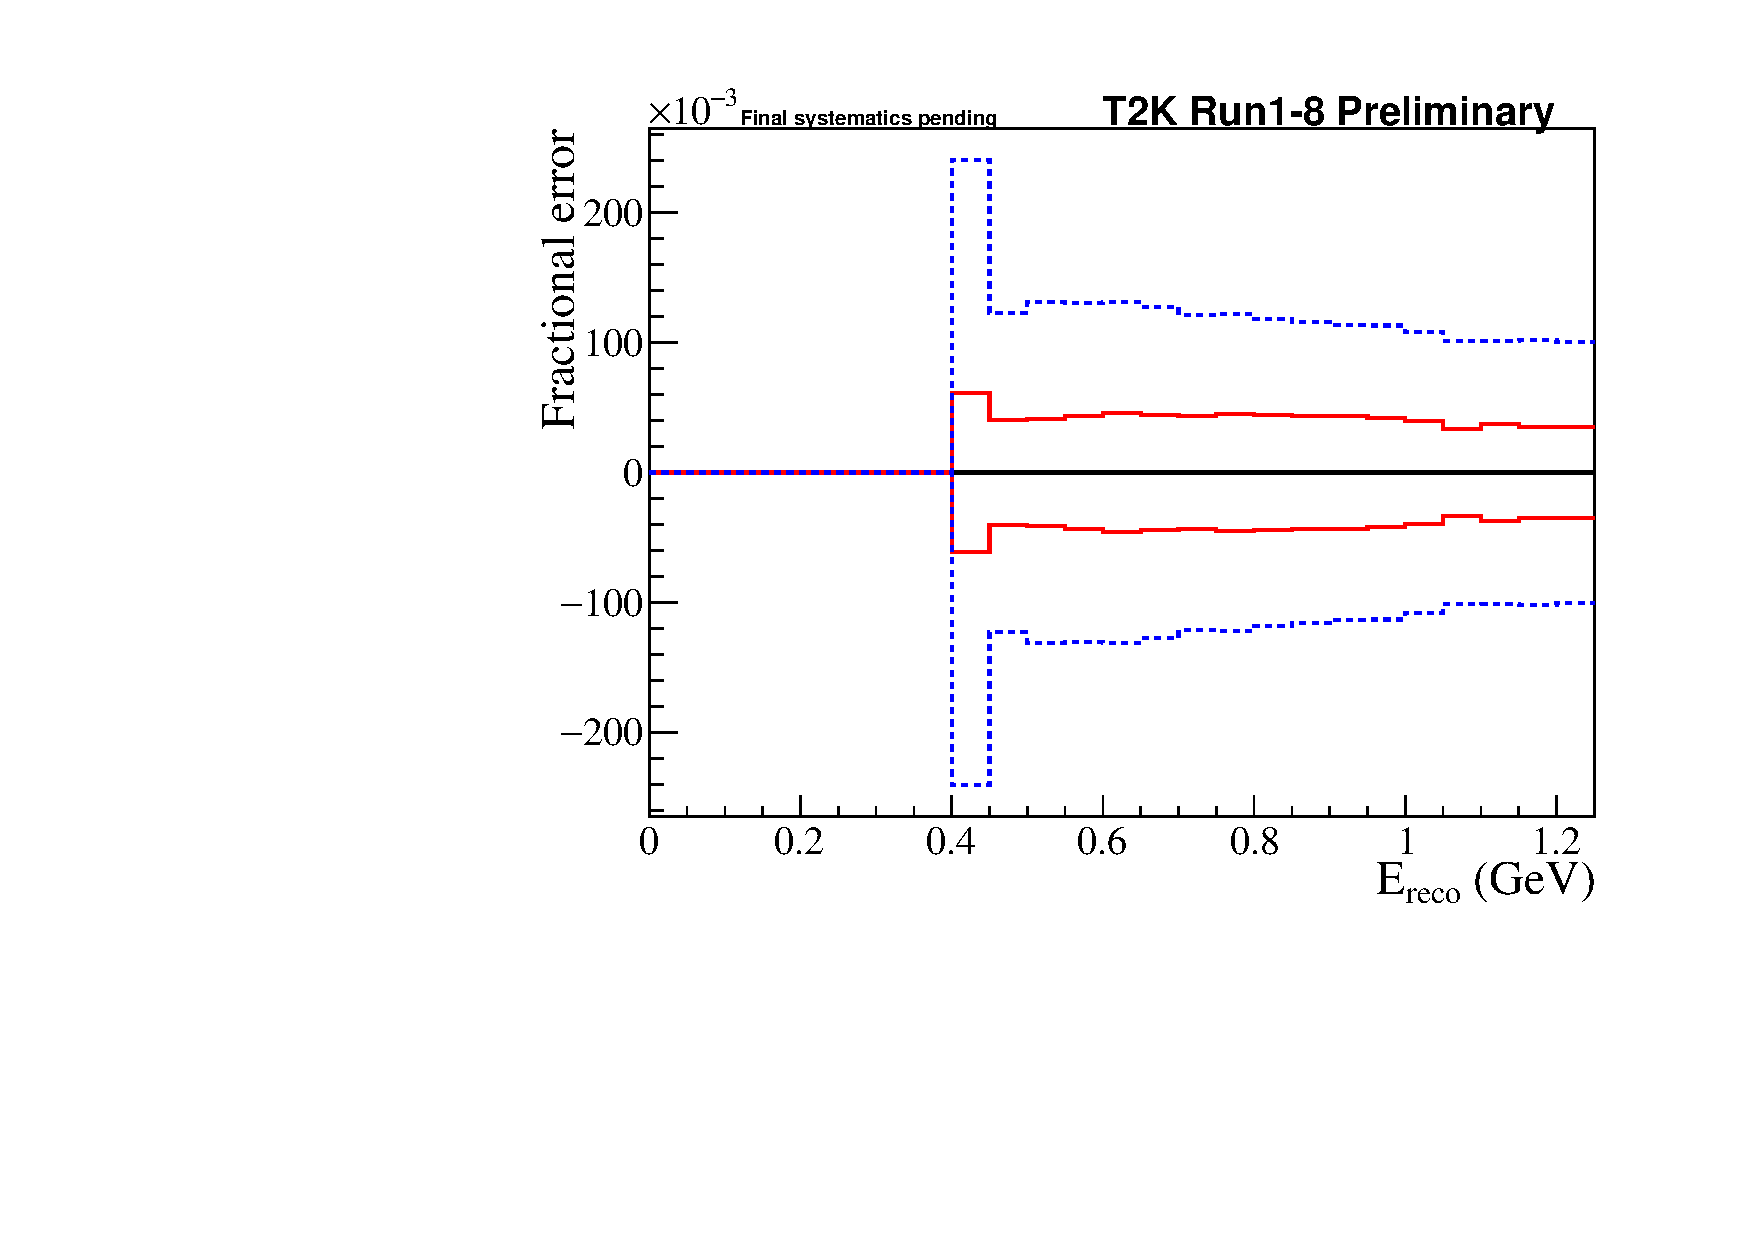
\includegraphics[width=0.9\textwidth]{systematics/envelopes/sk_errors/sk_error_table_MultiRe_banff_constrained_envelope_fractional}
		\caption{\nueCConepi-like, neutrino mode}
	\end{subfigure}
	\caption {
		Error envelopes (left) and fractional errors (right) for the reconstructed neutrino energy spectrum for the flux and constrained cross-section systematic parameters for pre-BANFF (blue) and post-BANFF (red) errors. \num{1e4} toys are generated for the Asimov data set A with randomized systematic parameters with correlations taken into account.
	}
	\label{fig:sk_envelopes_banff}
\end{figure*}
\clearpage

\begin{figure*}
	\center
	\begin{subfigure}[b]{0.49\textwidth}
		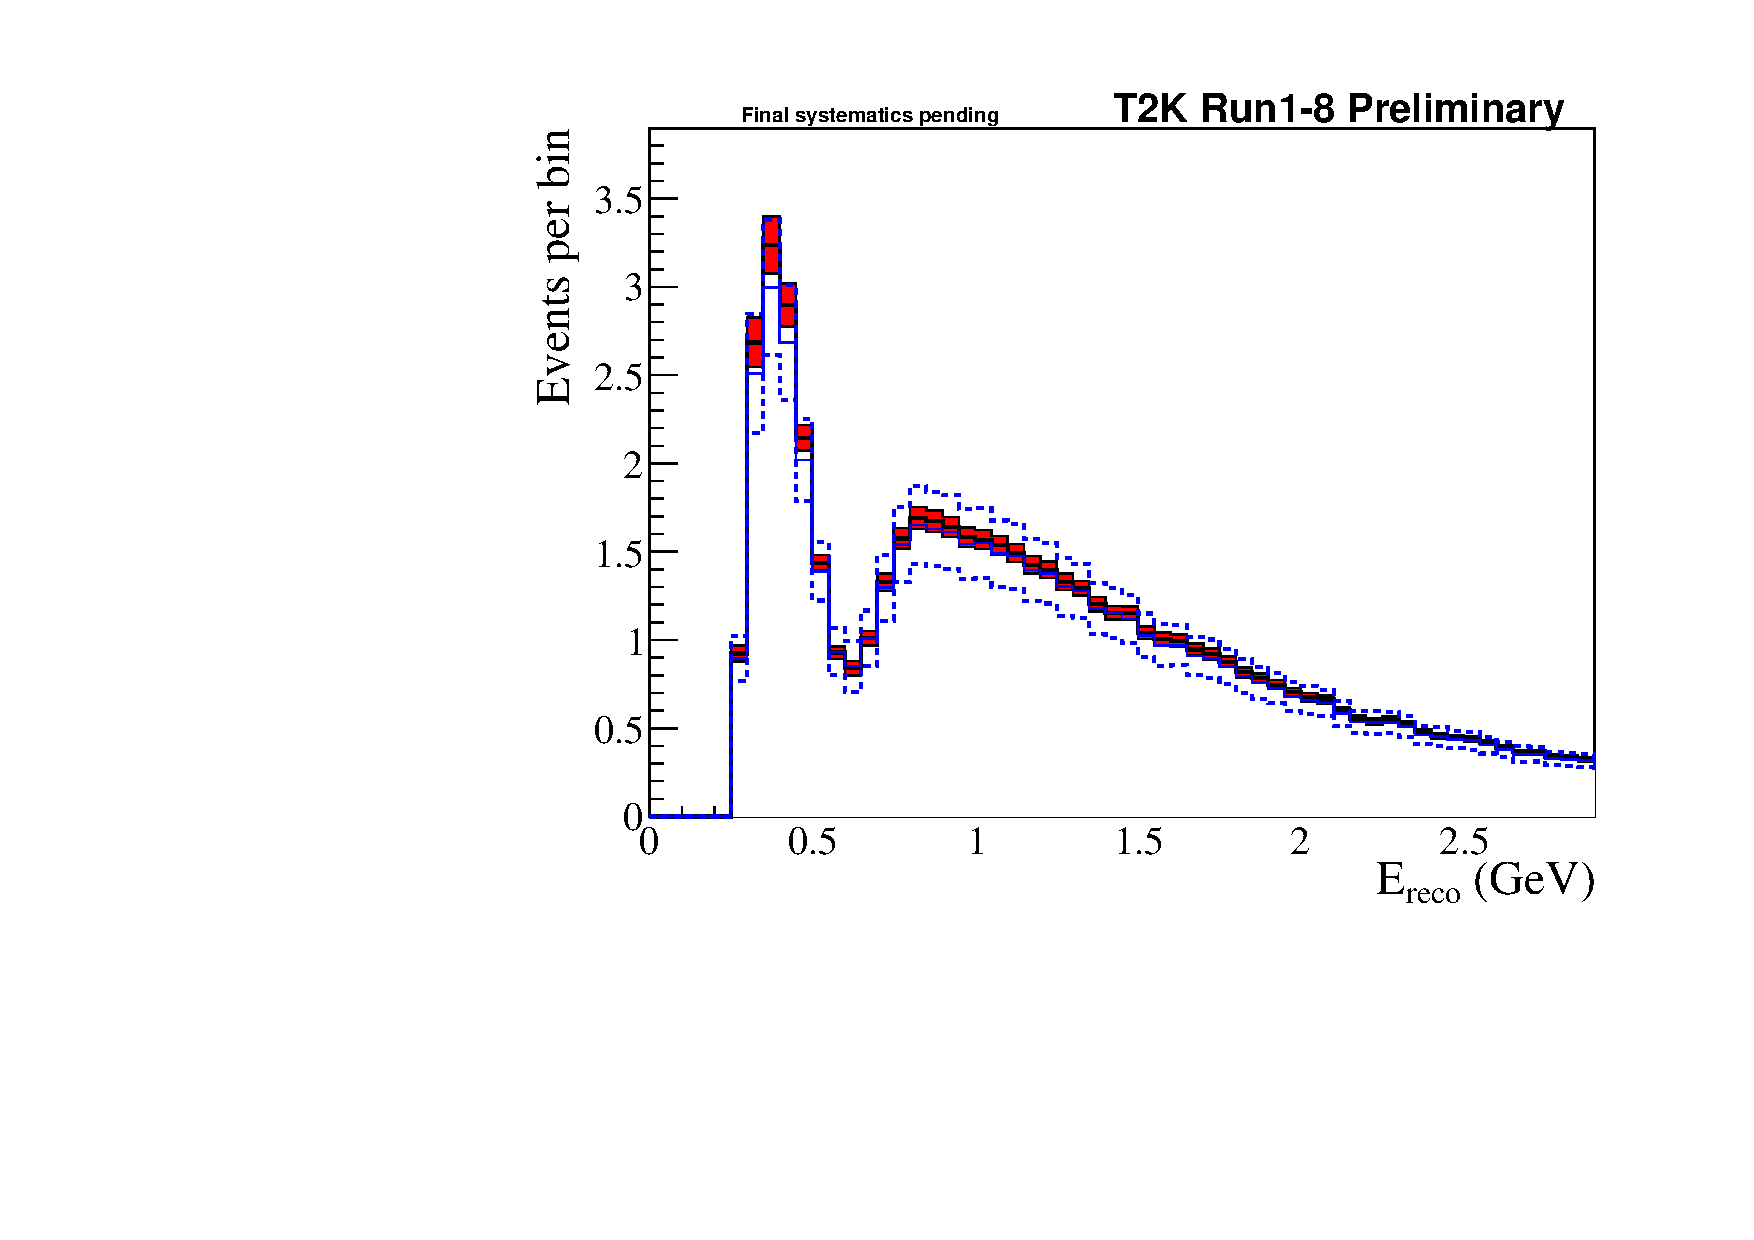
\includegraphics[width=0.9\textwidth]{systematics/envelopes/sk_errors/sk_error_table_RHC1Rmu_banff_constrained_envelope}
		\caption{Muon-like, antineutrino mode}
	\end{subfigure}
	\begin{subfigure}[b]{0.49\textwidth}
		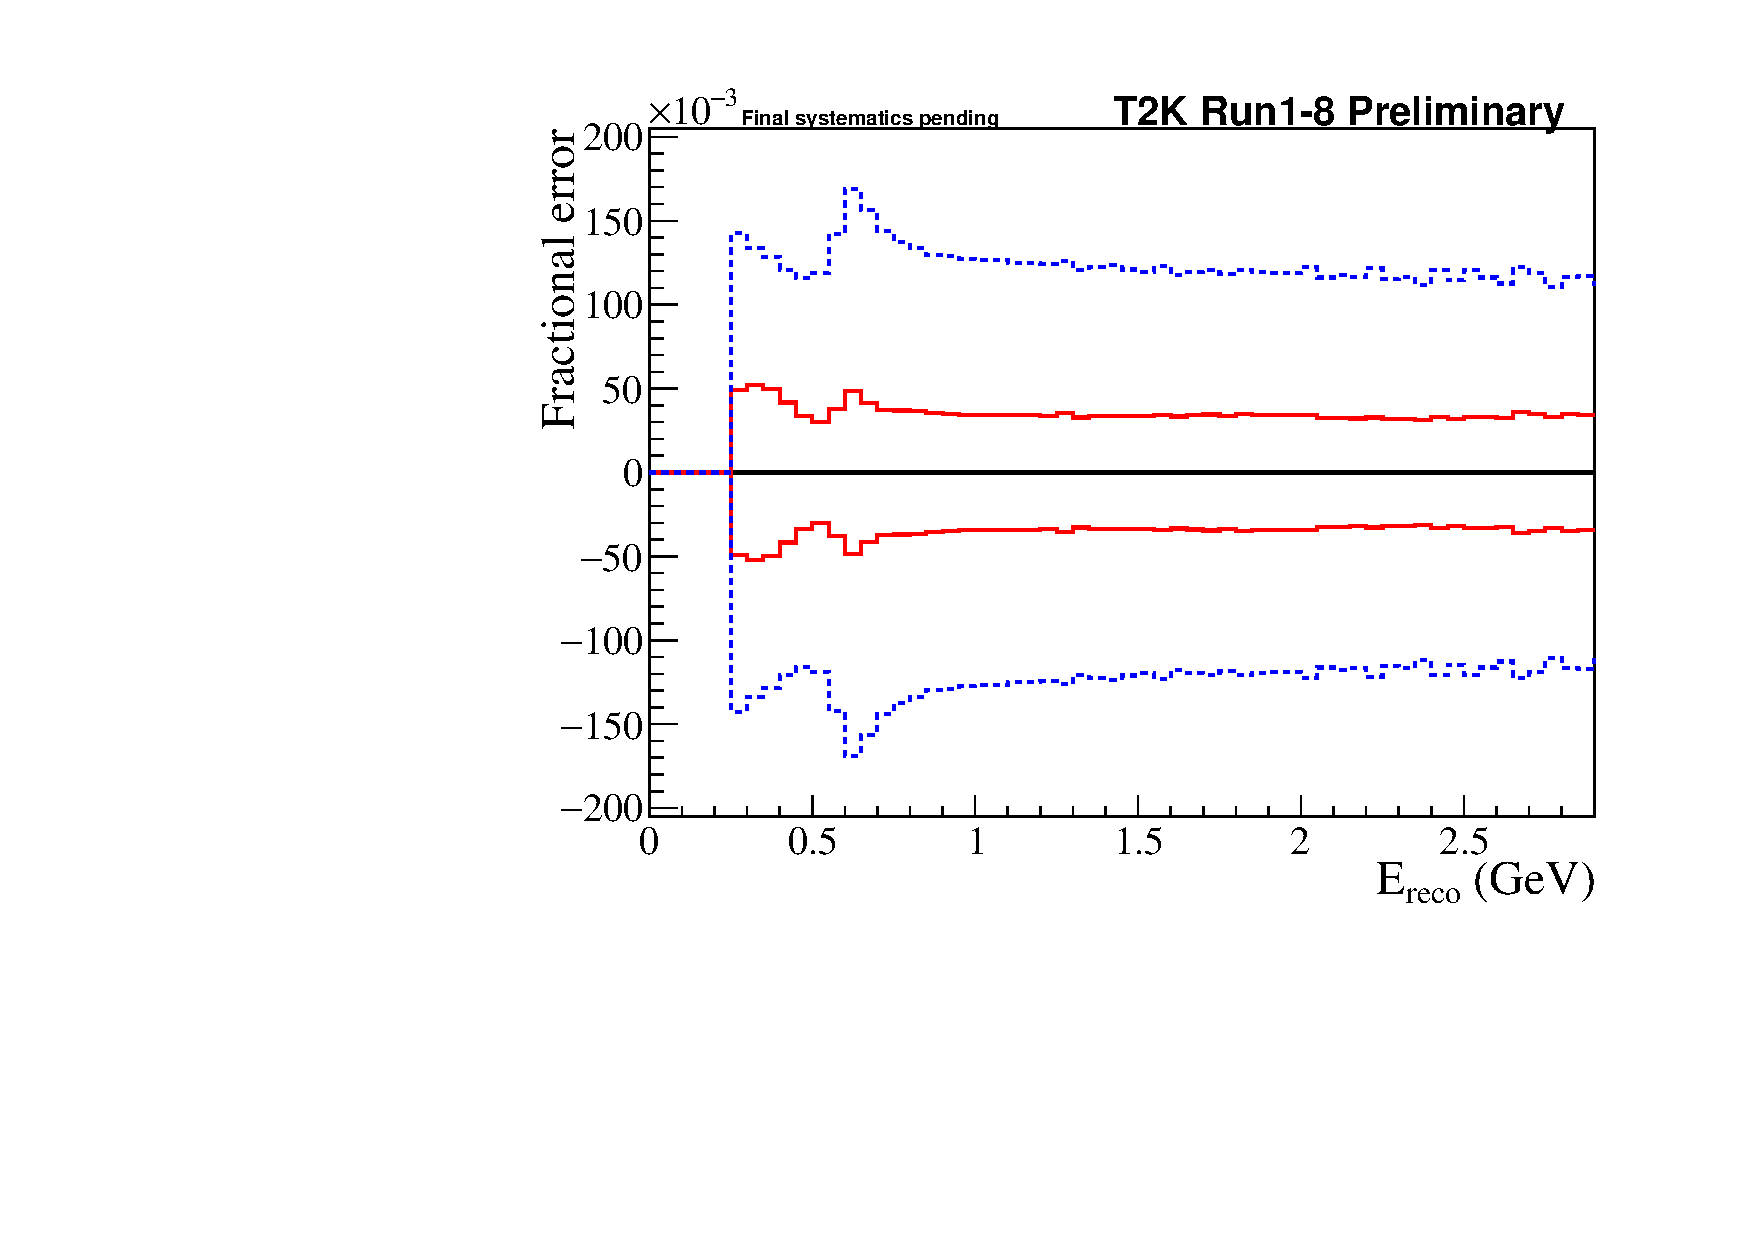
\includegraphics[width=0.9\textwidth]{systematics/envelopes/sk_errors/sk_error_table_RHC1Rmu_banff_constrained_envelope_fractional}
		\caption{Muon-like, antineutrino mode}
	\end{subfigure}
	\begin{subfigure}[b]{0.49\textwidth}
		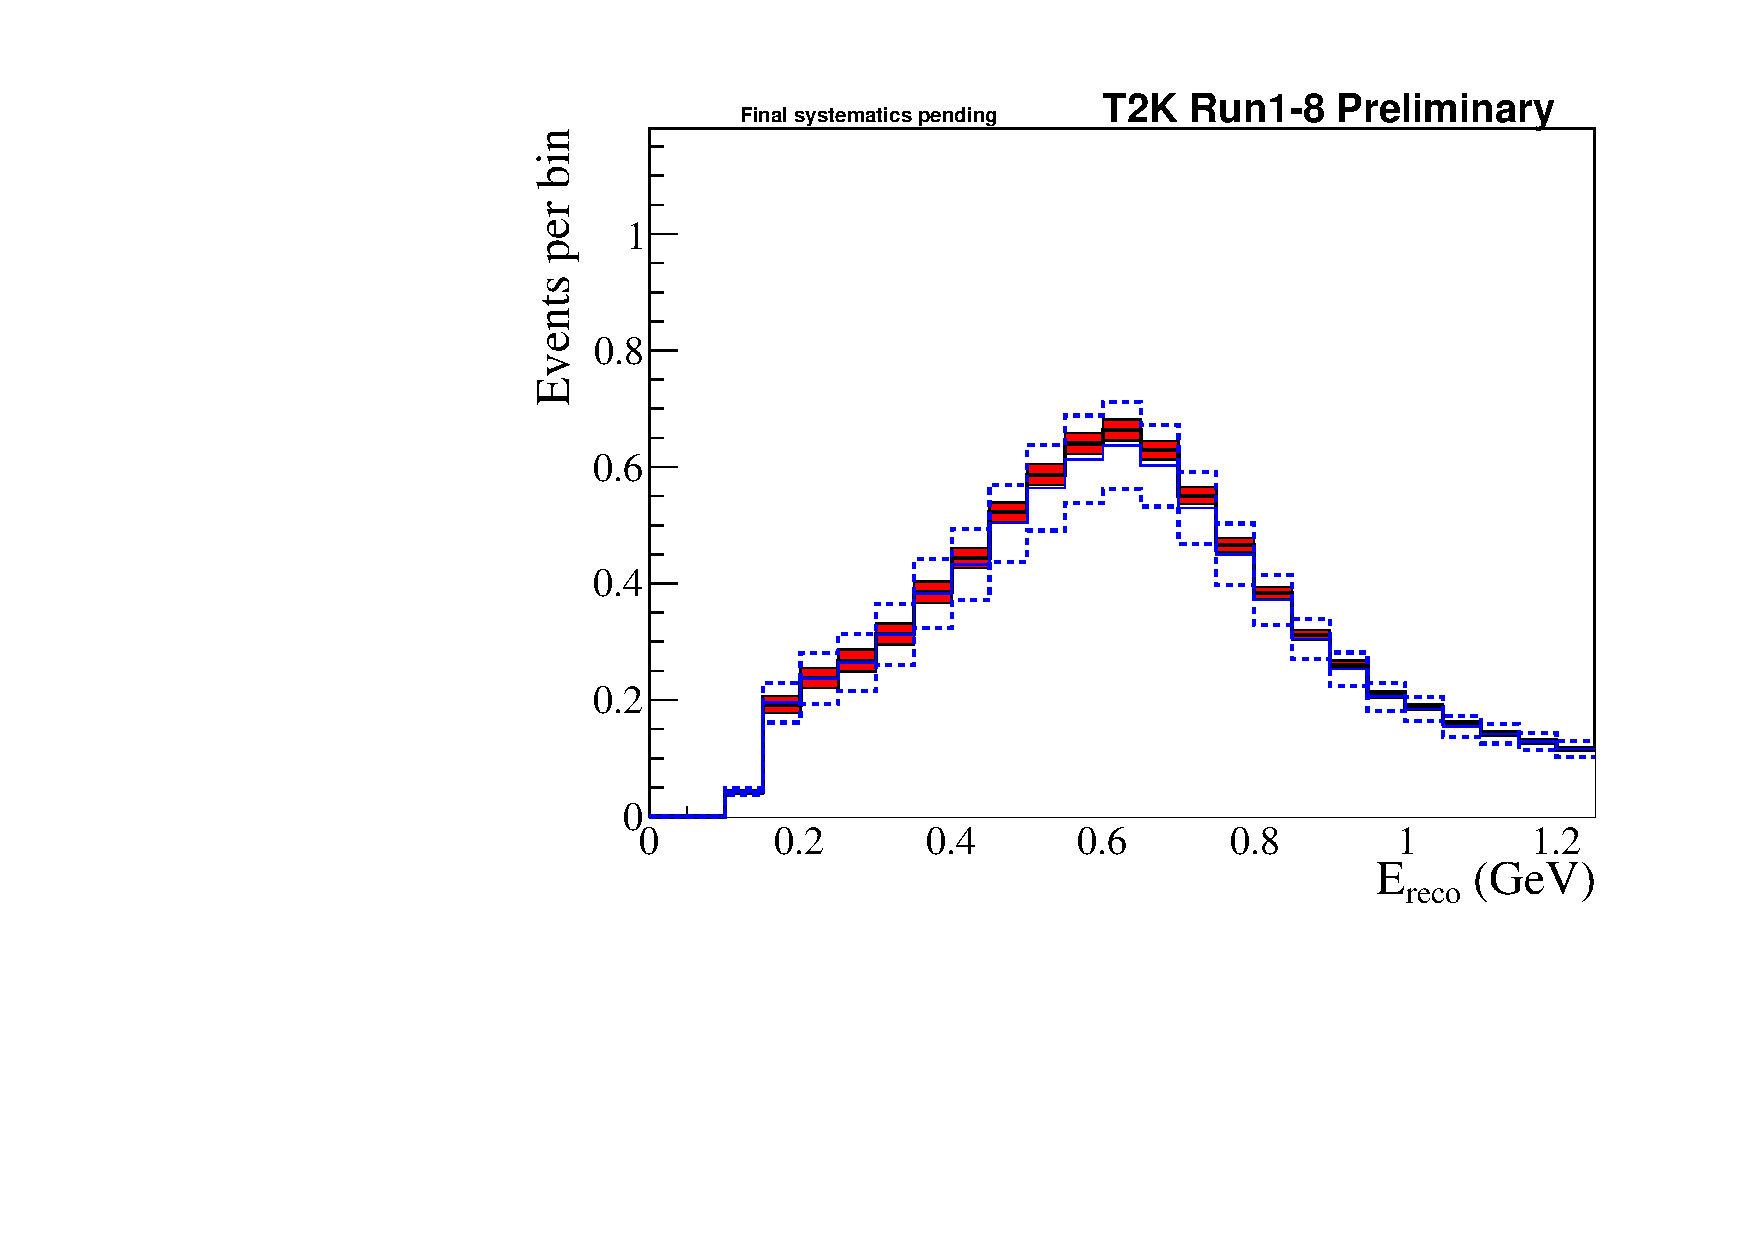
\includegraphics[width=0.9\textwidth]{systematics/envelopes/sk_errors/sk_error_table_RHC1Re_banff_constrained_envelope}
		\caption{Electron-like antineutrino mode}
	\end{subfigure}
	\begin{subfigure}[b]{0.49\textwidth}
		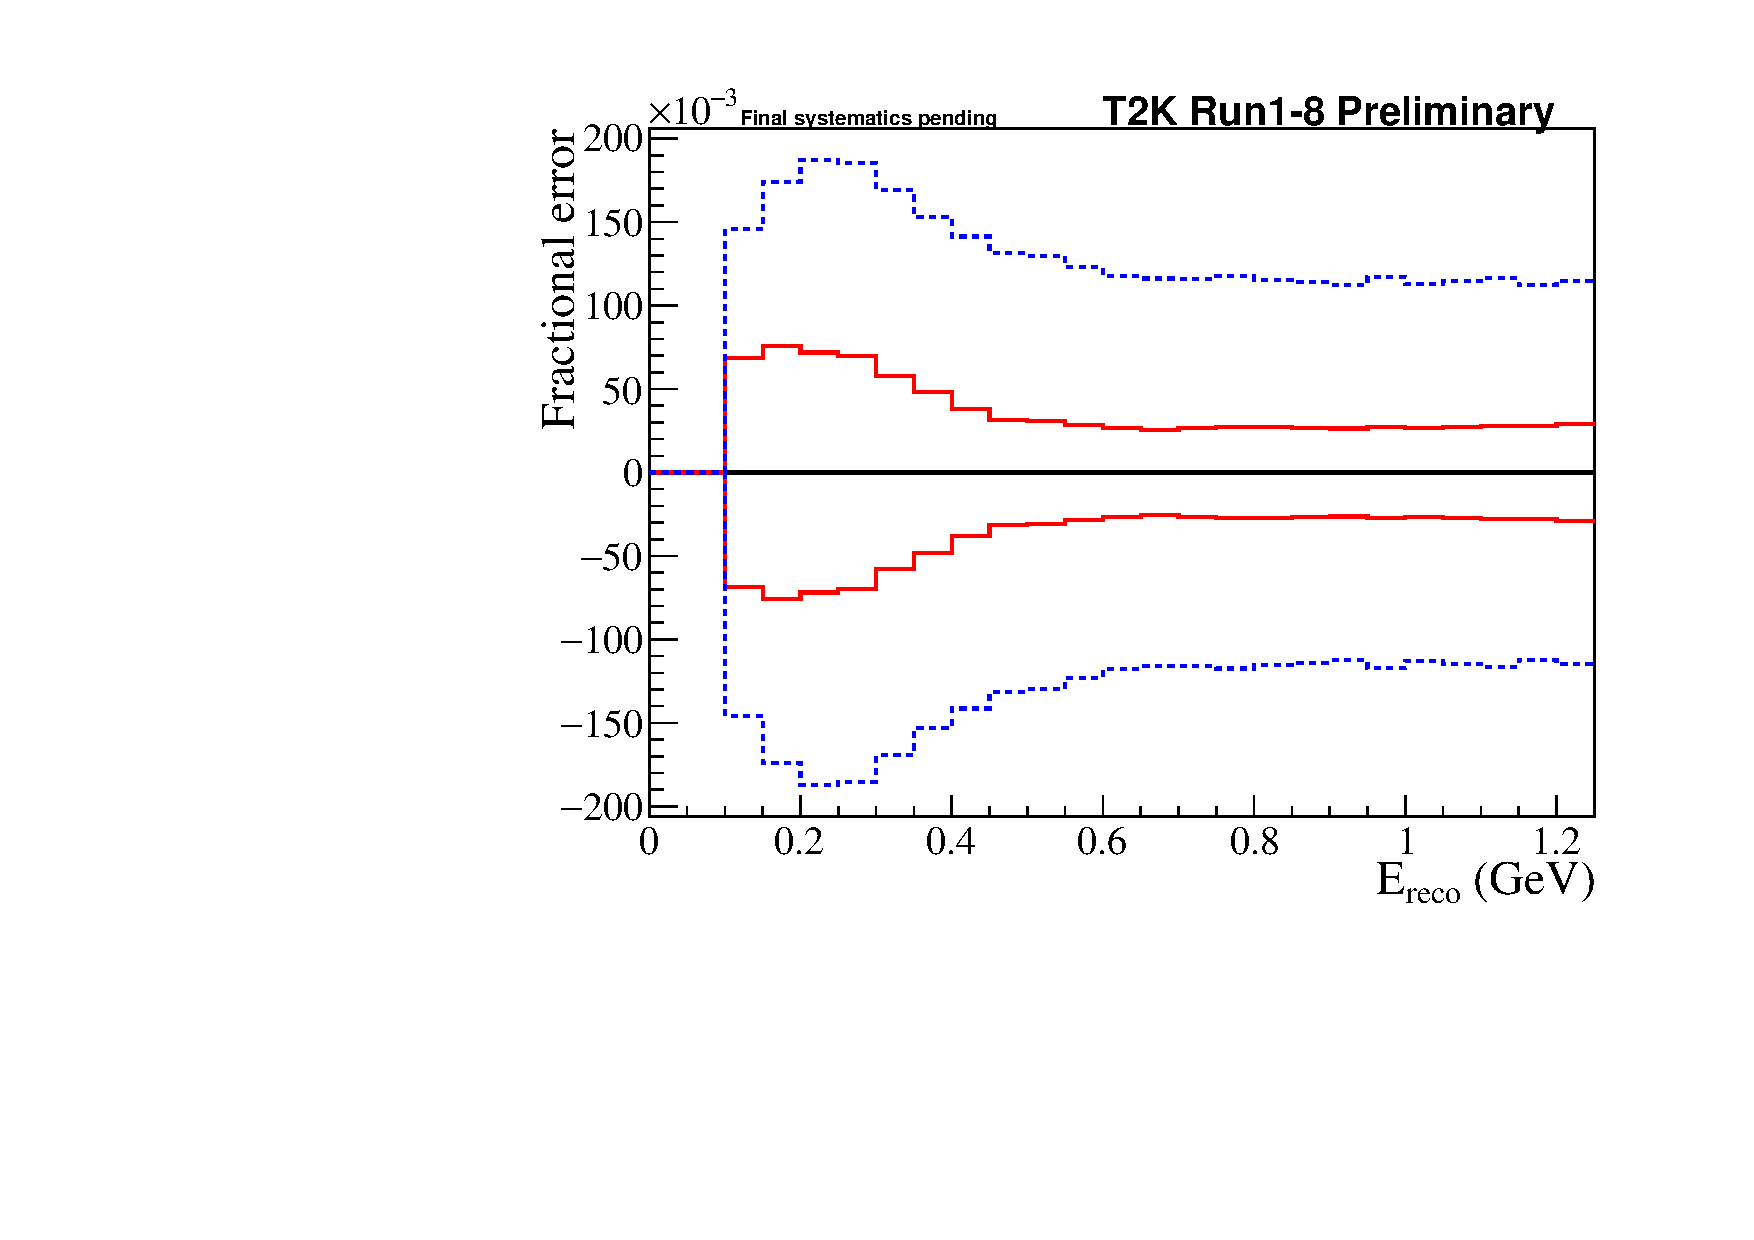
\includegraphics[width=0.9\textwidth]{systematics/envelopes/sk_errors/sk_error_table_RHC1Re_banff_constrained_envelope_fractional}
		\caption{Electron-like antineutrino mode}
	\end{subfigure}
	\caption {
		Error envelopes (left) and fractional error (right) for the reconstructed neutrino energy spectrum for the flux and constrained cross-section systematic parameters for pre-BANFF (blue) and post-BANFF (red) errors. \num{1e4} toys are generated for the Asimov data set A with randomized systematic parameters with correlations taken into account.
	}
	\label{fig:sk_envelopes_banff_b}
\end{figure*}
\clearpage
\begin{figure*}
	\center
	\begin{subfigure}[b]{0.49\textwidth}
		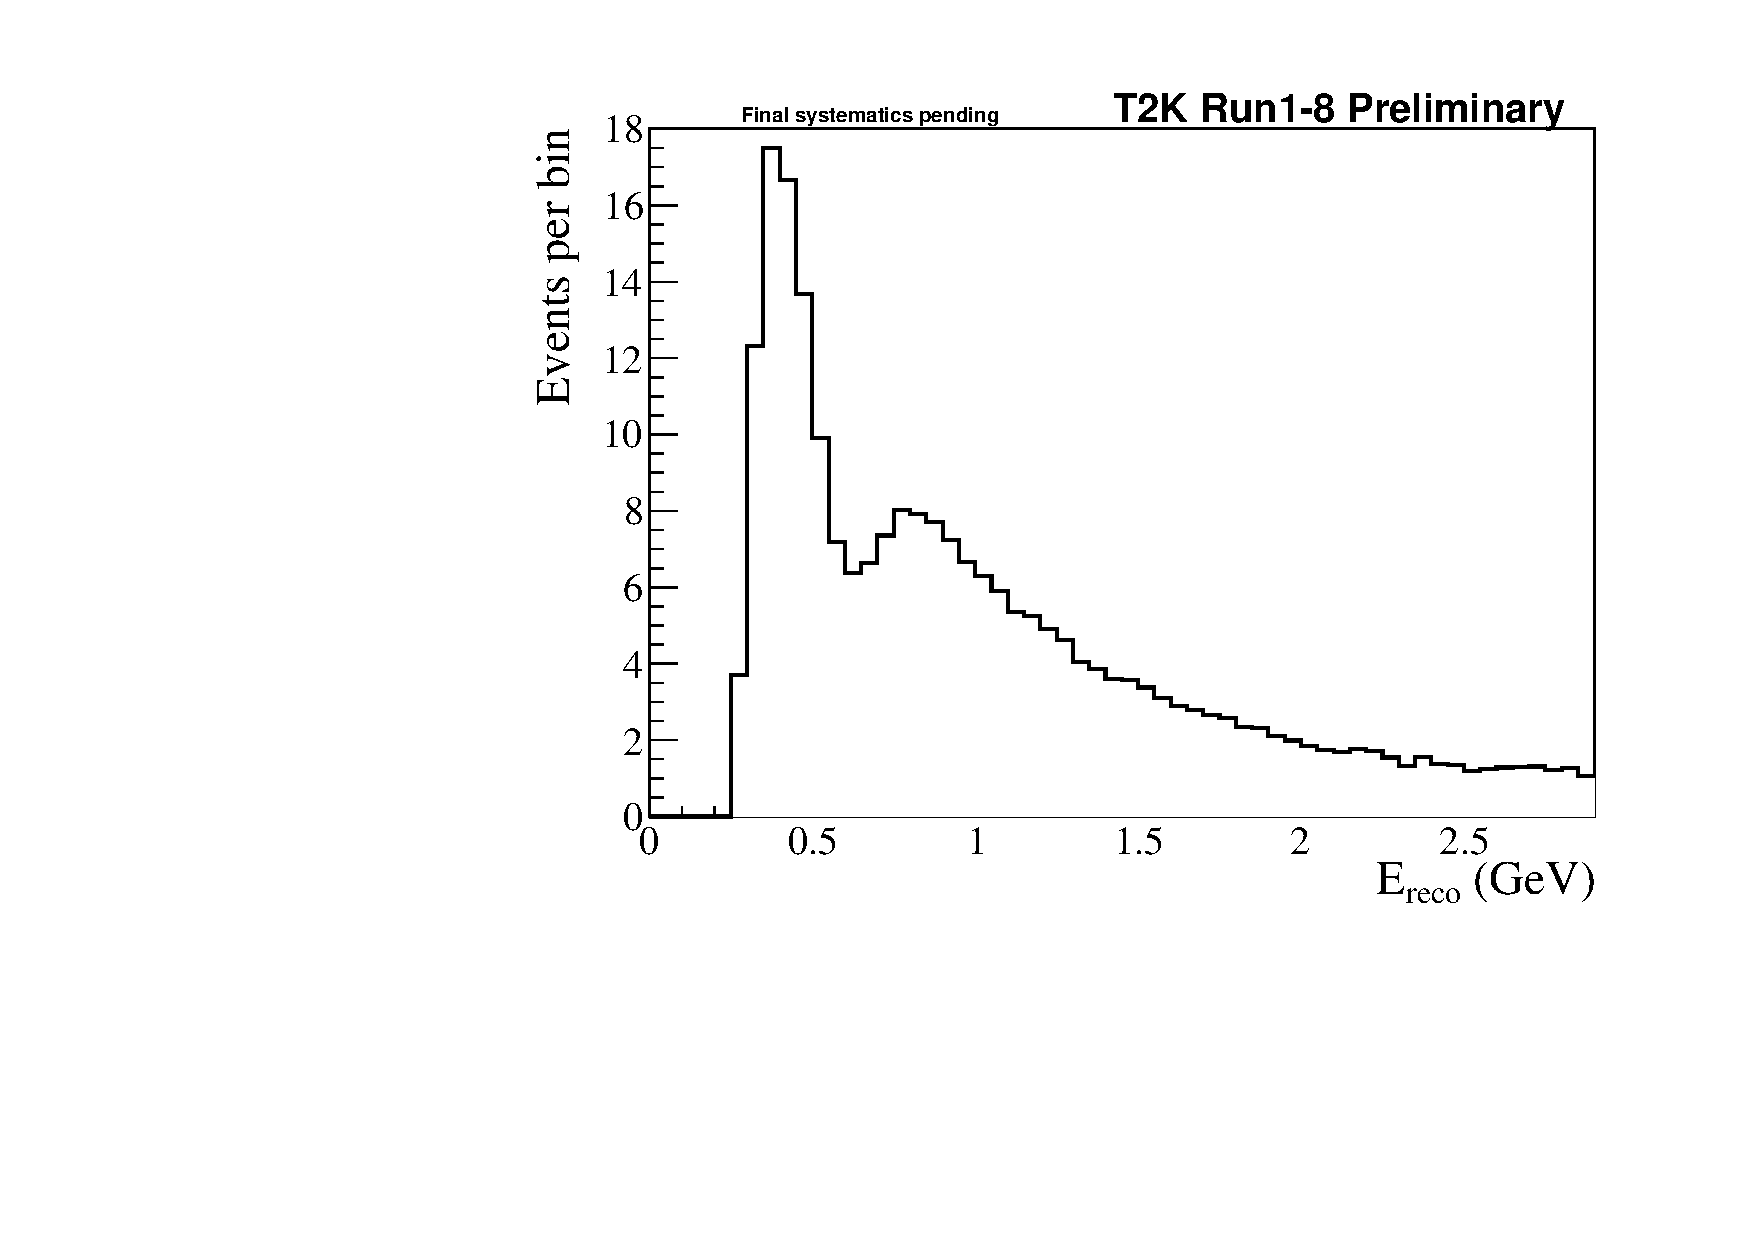
\includegraphics[width=0.9\textwidth]{systematics/envelopes/sk_errors/sk_error_table_1Rmu_xsec_nue_envelope}
		\caption{Muon-like, neutrino mode}
	\end{subfigure}
	\begin{subfigure}[b]{0.49\textwidth}
		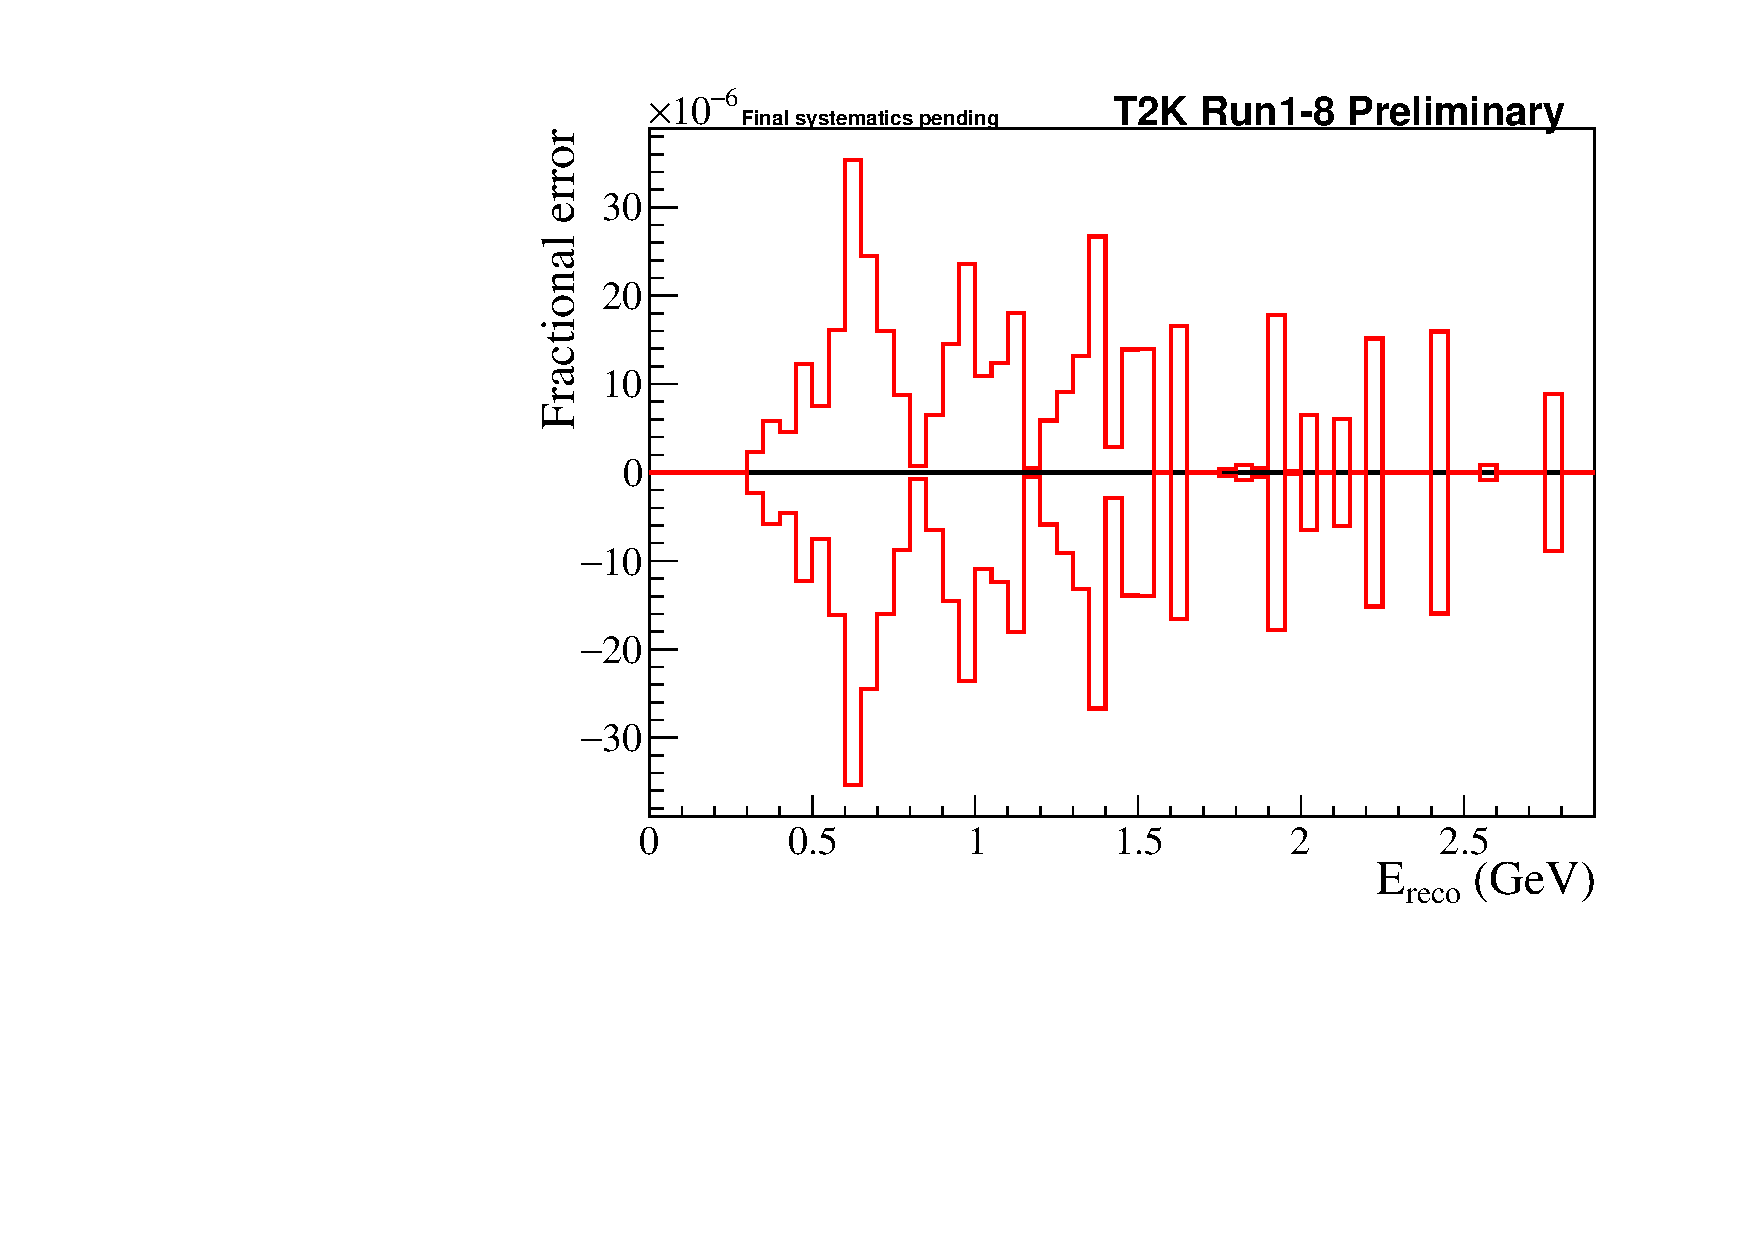
\includegraphics[width=0.9\textwidth]{systematics/envelopes/sk_errors/sk_error_table_1Rmu_xsec_nue_envelope_fractional}
		\caption{Muon-like, neutrino mode}
	\end{subfigure}
	\begin{subfigure}[b]{0.49\textwidth}
		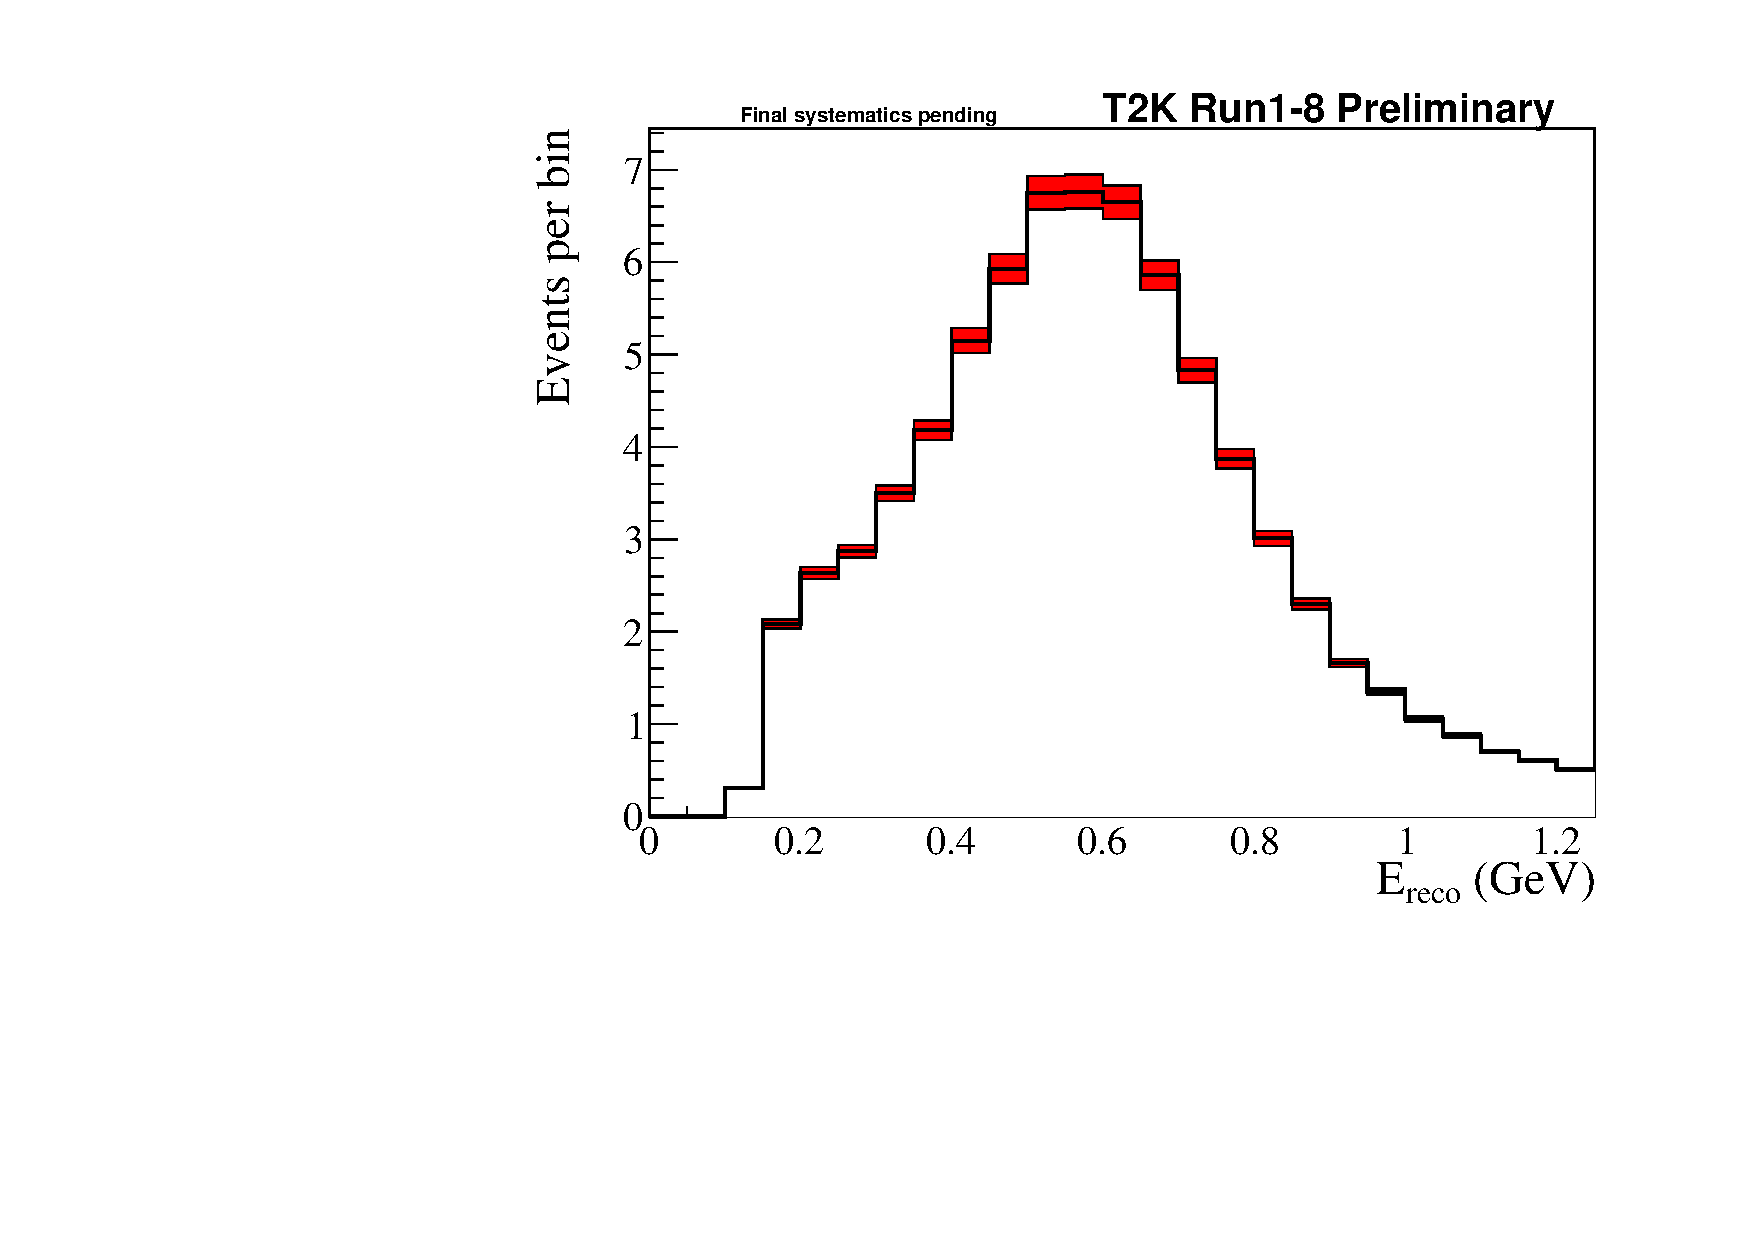
\includegraphics[width=0.9\textwidth]{systematics/envelopes/sk_errors/sk_error_table_1Re_xsec_nue_envelope}
		\caption{Electron-like, neutrino mode}
	\end{subfigure}
	\begin{subfigure}[b]{0.49\textwidth}
		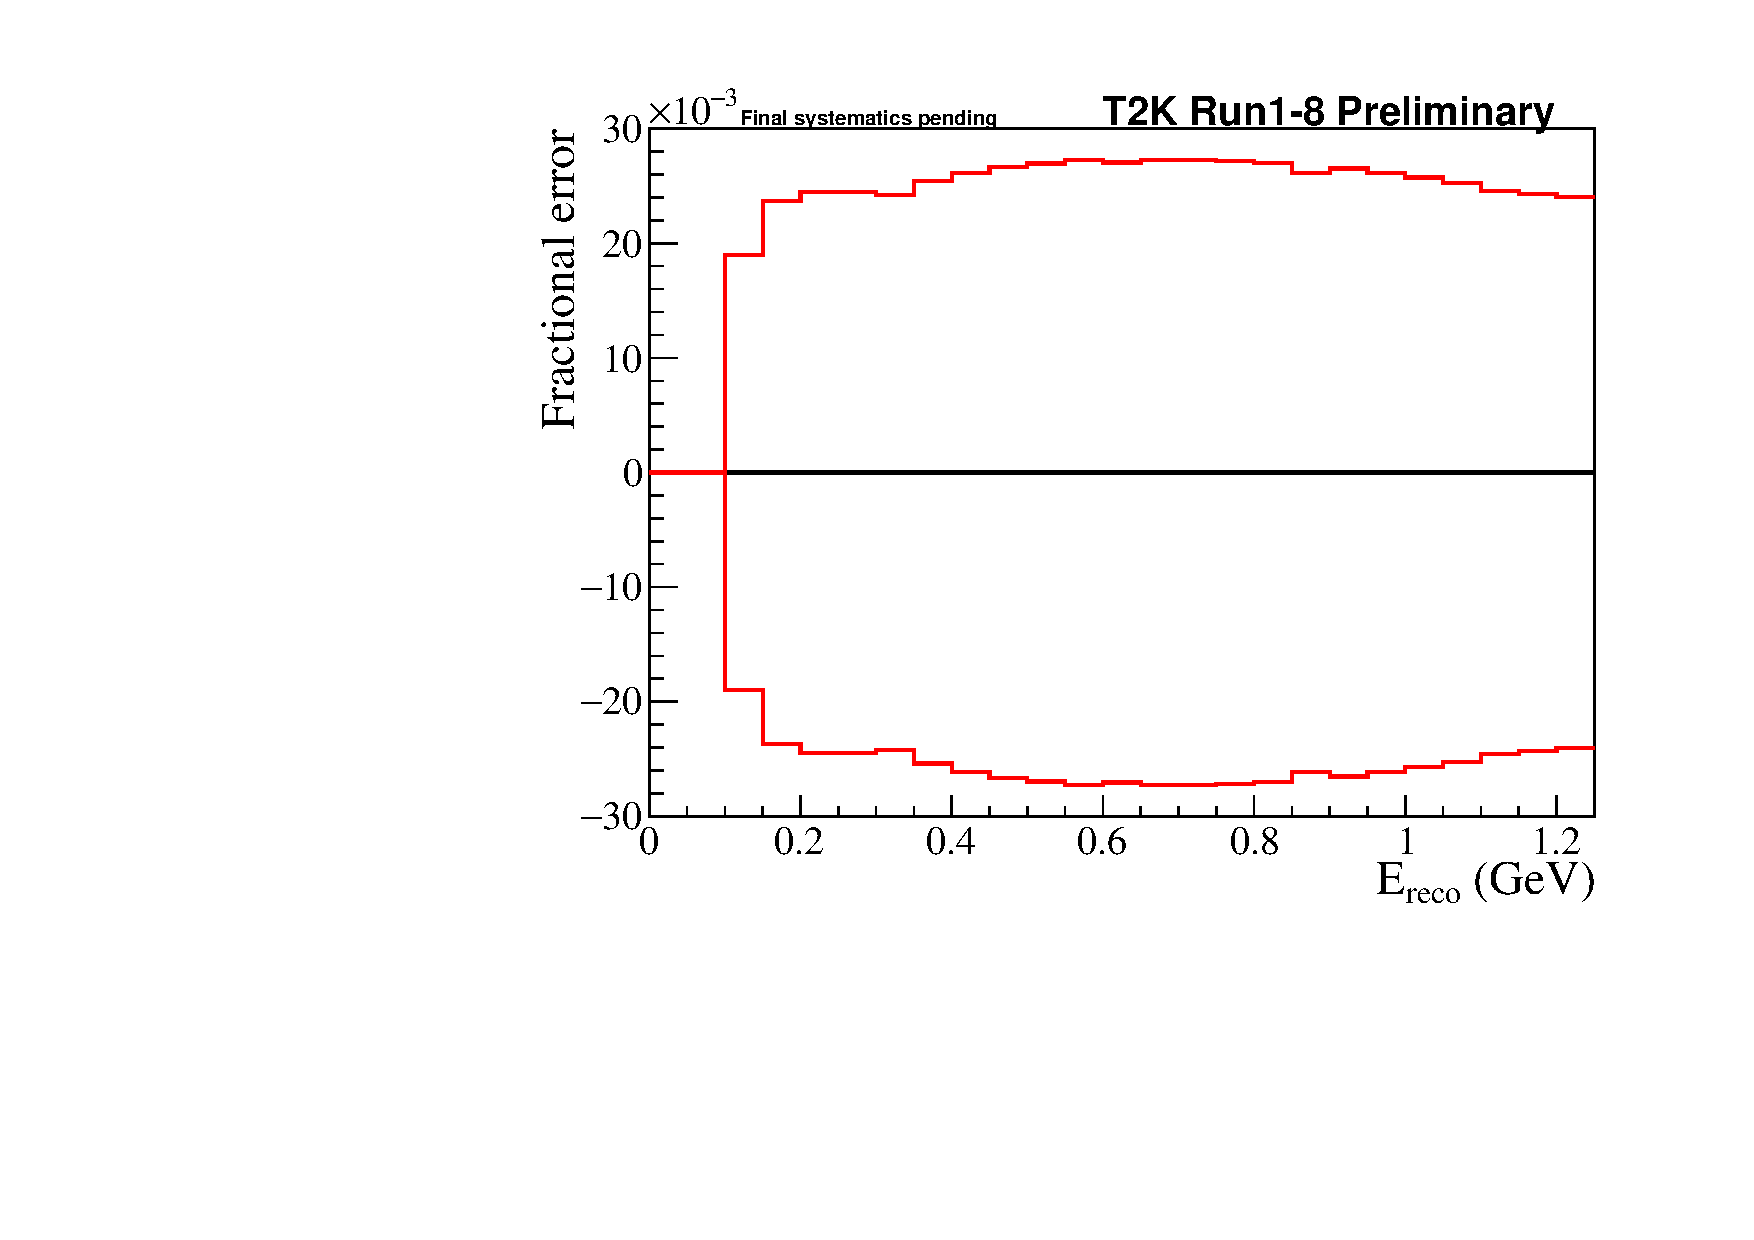
\includegraphics[width=0.9\textwidth]{systematics/envelopes/sk_errors/sk_error_table_1Re_xsec_nue_envelope_fractional}
		\caption{Electron-like, neutrino mode}
	\end{subfigure}
	\begin{subfigure}[b]{0.49\textwidth}
		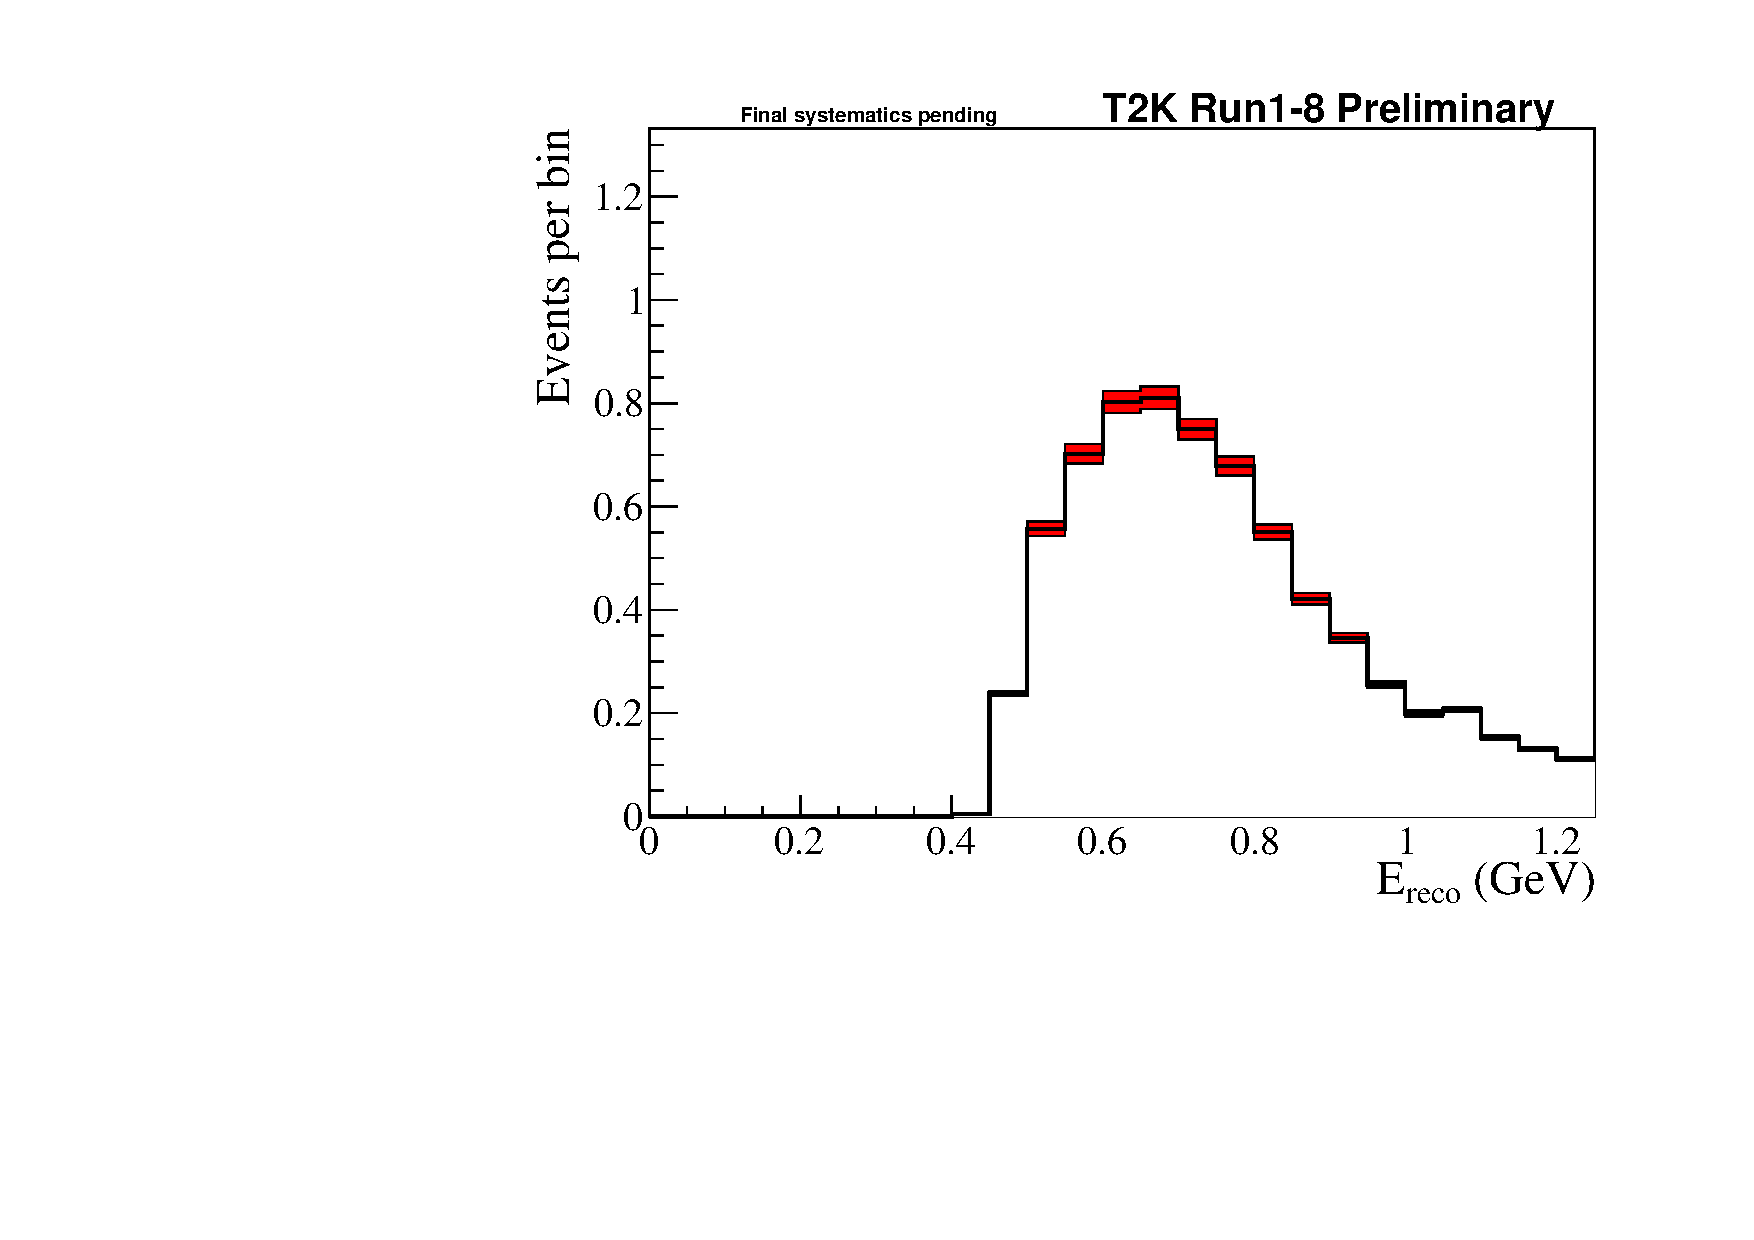
\includegraphics[width=0.9\textwidth]{systematics/envelopes/sk_errors/sk_error_table_MultiRe_xsec_nue_envelope}
		\caption{\nueCConepi-like, neutrino mode}
	\end{subfigure}
	\begin{subfigure}[b]{0.49\textwidth}
		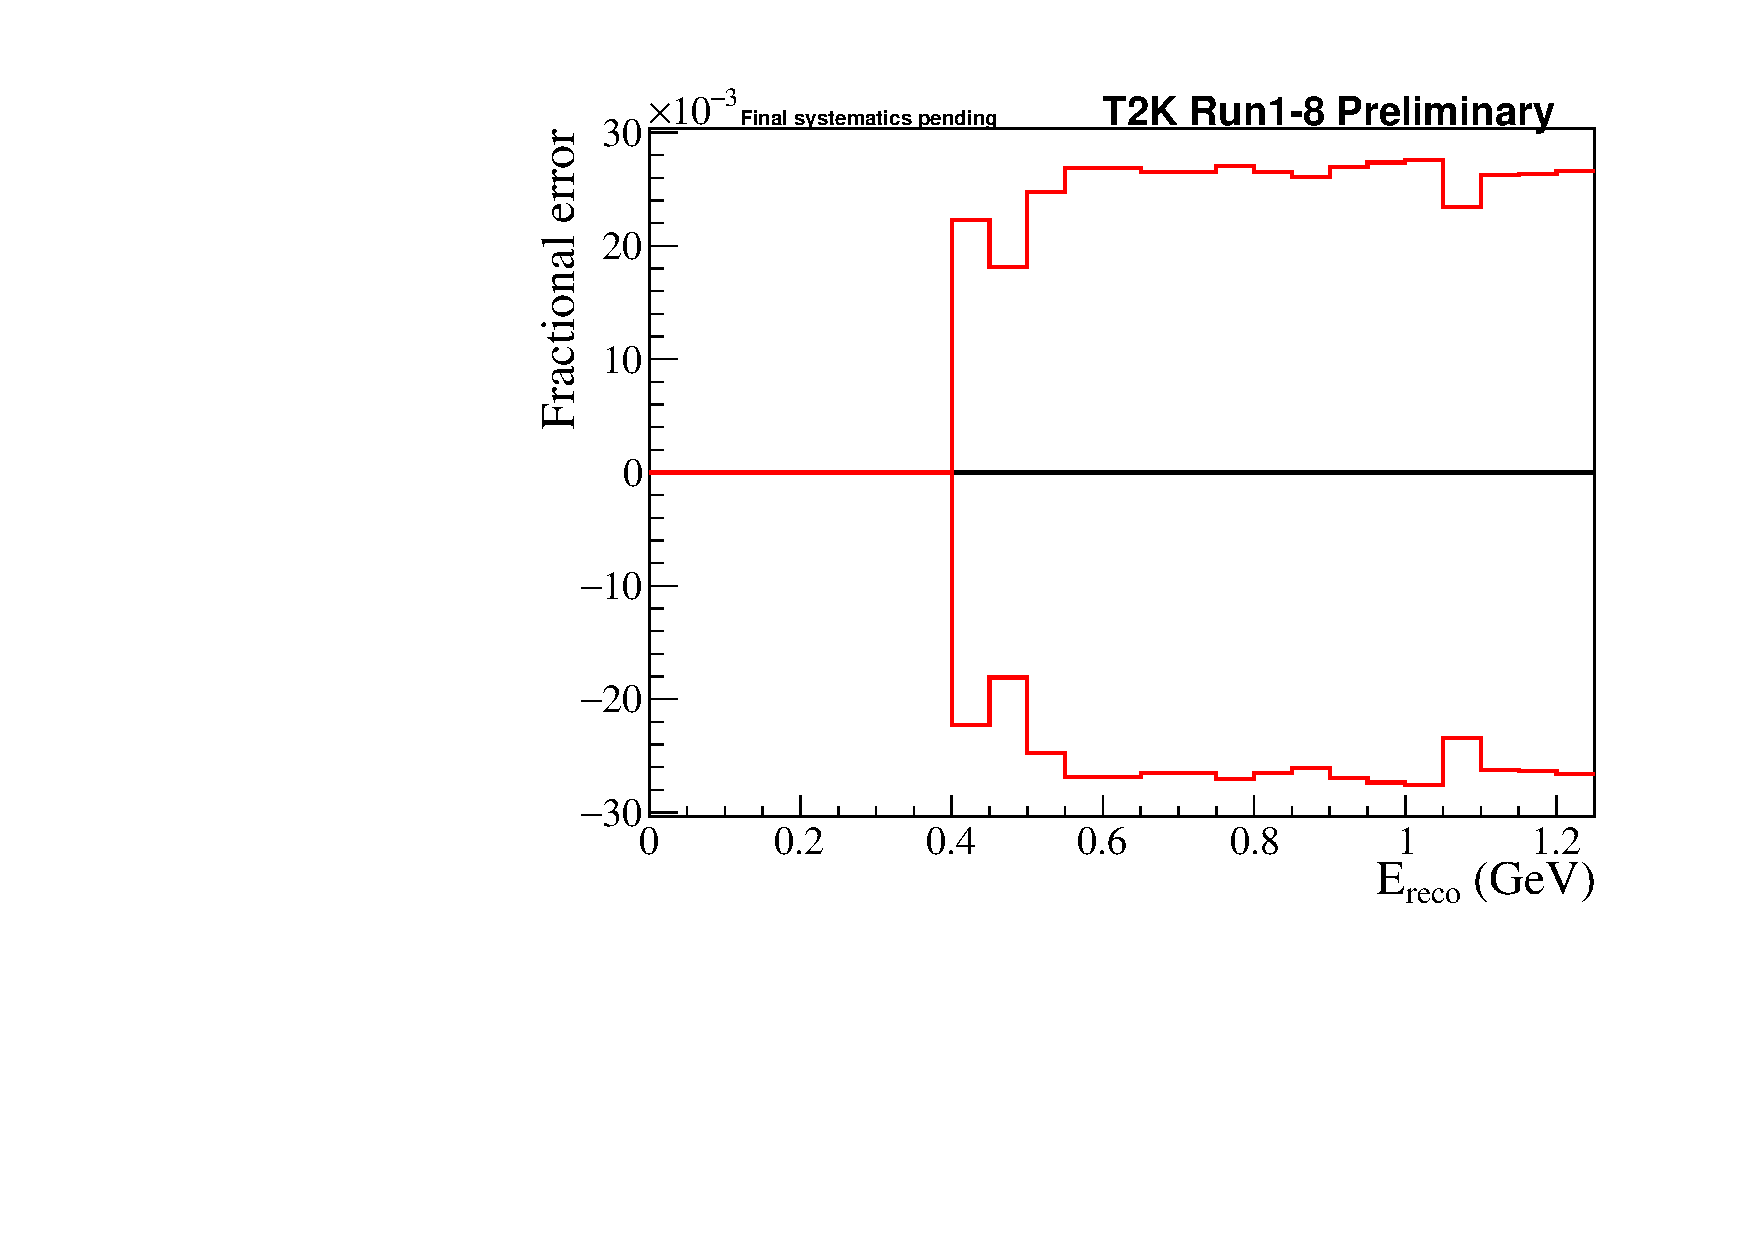
\includegraphics[width=0.9\textwidth]{systematics/envelopes/sk_errors/sk_error_table_MultiRe_xsec_nue_envelope_fractional}
		\caption{\nueCConepi-like, neutrino mode}
	\end{subfigure}
	\caption {
		Error envelopes (left) and fractional errors (right) for the reconstructed neutrino energy spectrum for the unconstrained electron neutrino cross-section systematic parameters. \num{1e4} toys are generated for the Asimov data set A with randomized systematic parameters with correlations taken into account.
	}
	\label{fig:sk_envelopes_xsec_nue}
\end{figure*}
\clearpage

\begin{figure*}
	\center
	\begin{subfigure}[b]{0.49\textwidth}
		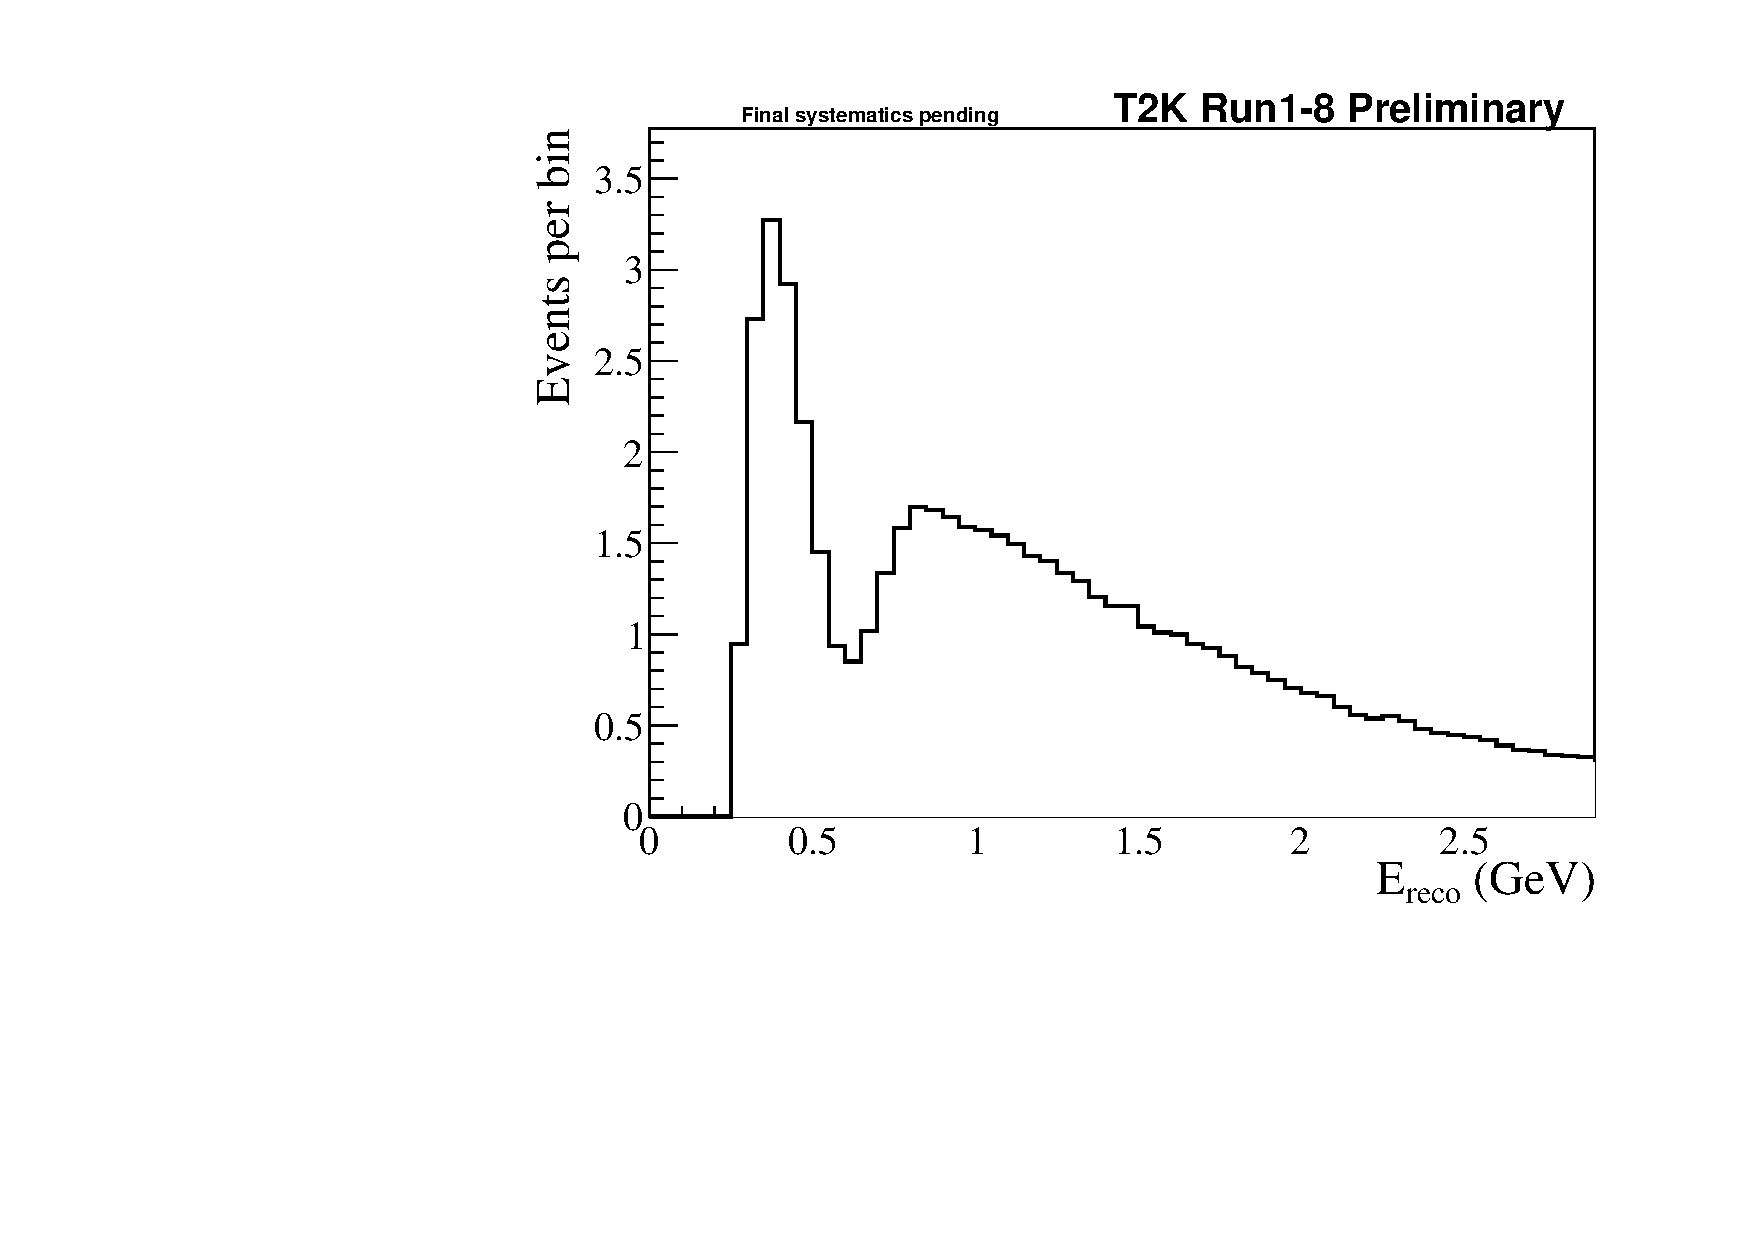
\includegraphics[width=0.9\textwidth]{systematics/envelopes/sk_errors/sk_error_table_RHC1Rmu_xsec_nue_envelope}
		\caption{Muon-like, antineutrino mode}
	\end{subfigure}
	\begin{subfigure}[b]{0.49\textwidth}
		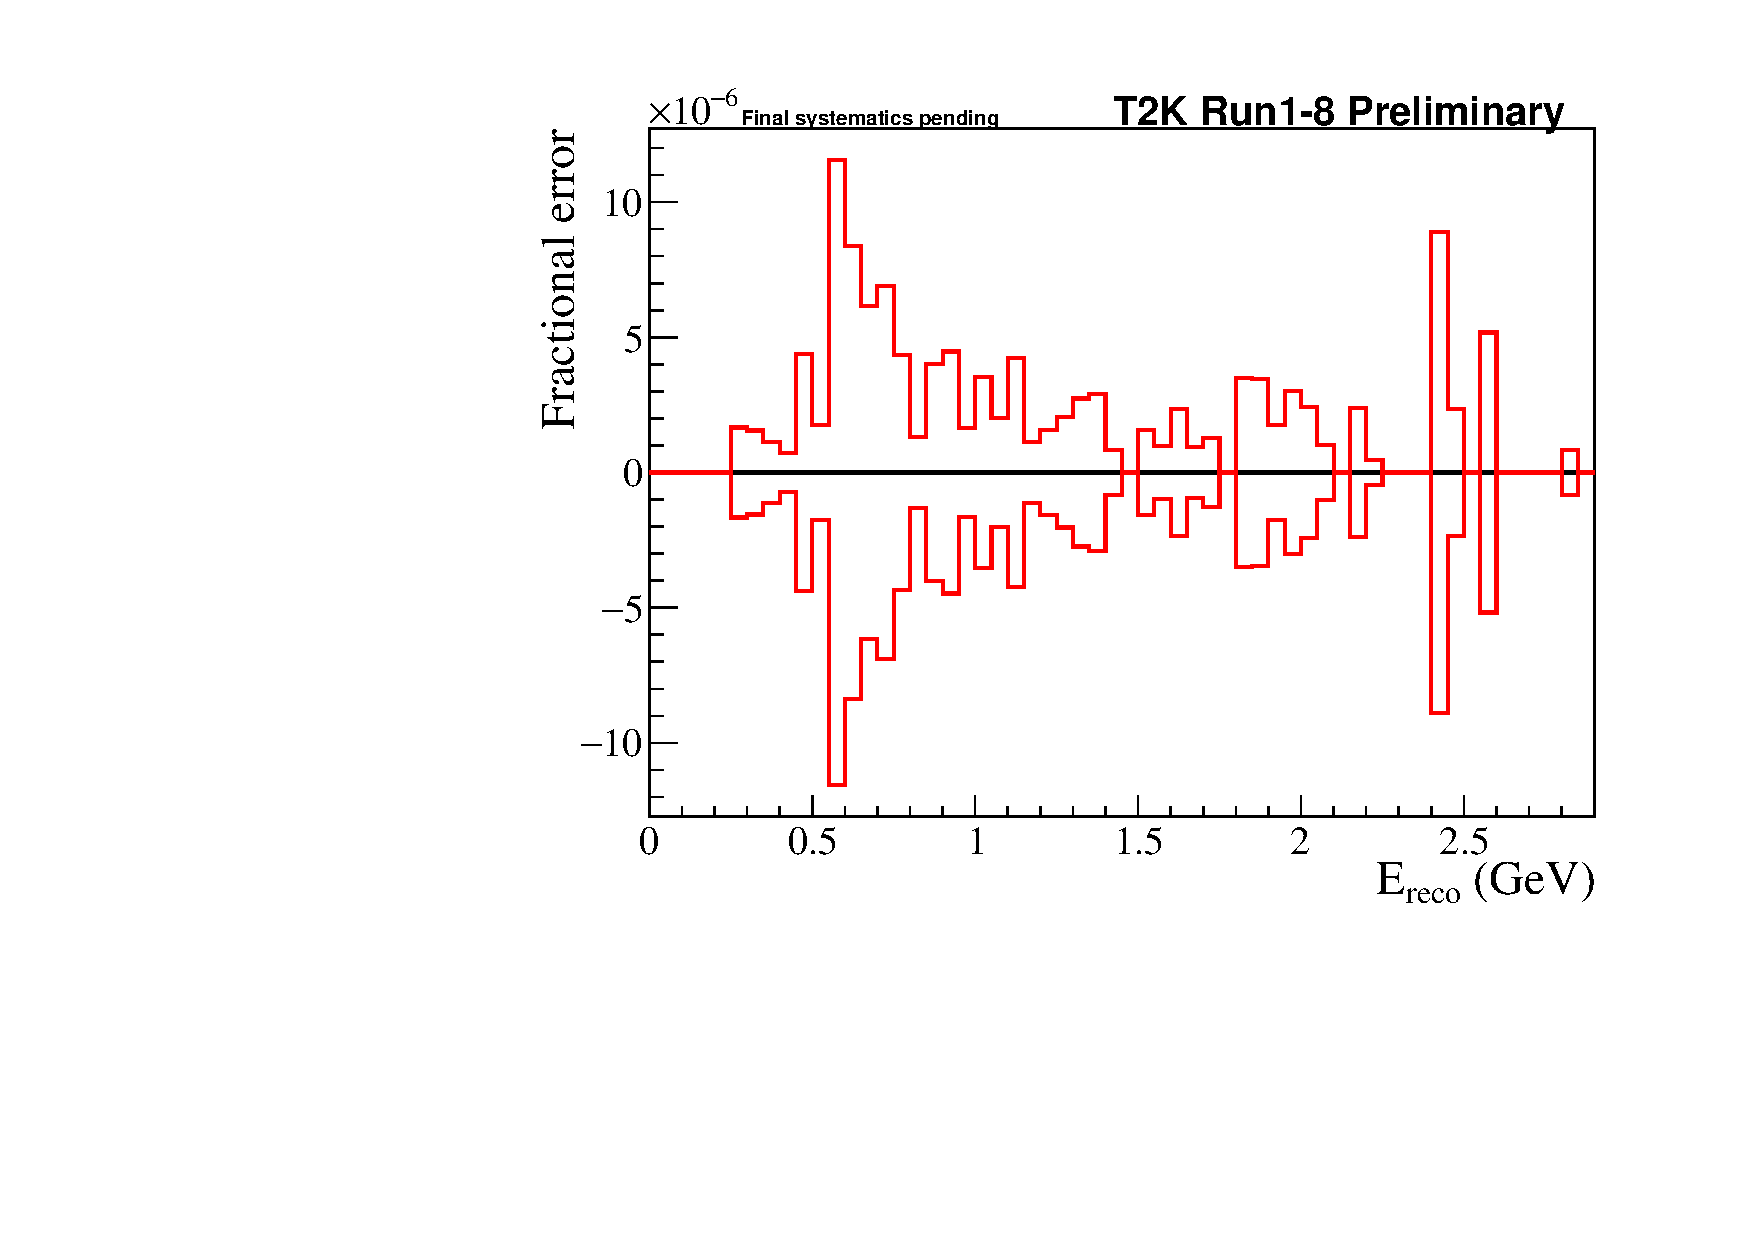
\includegraphics[width=0.9\textwidth]{systematics/envelopes/sk_errors/sk_error_table_RHC1Rmu_xsec_nue_envelope_fractional}
		\caption{Muon-like, antineutrino mode}
	\end{subfigure}
	\begin{subfigure}[b]{0.49\textwidth}
		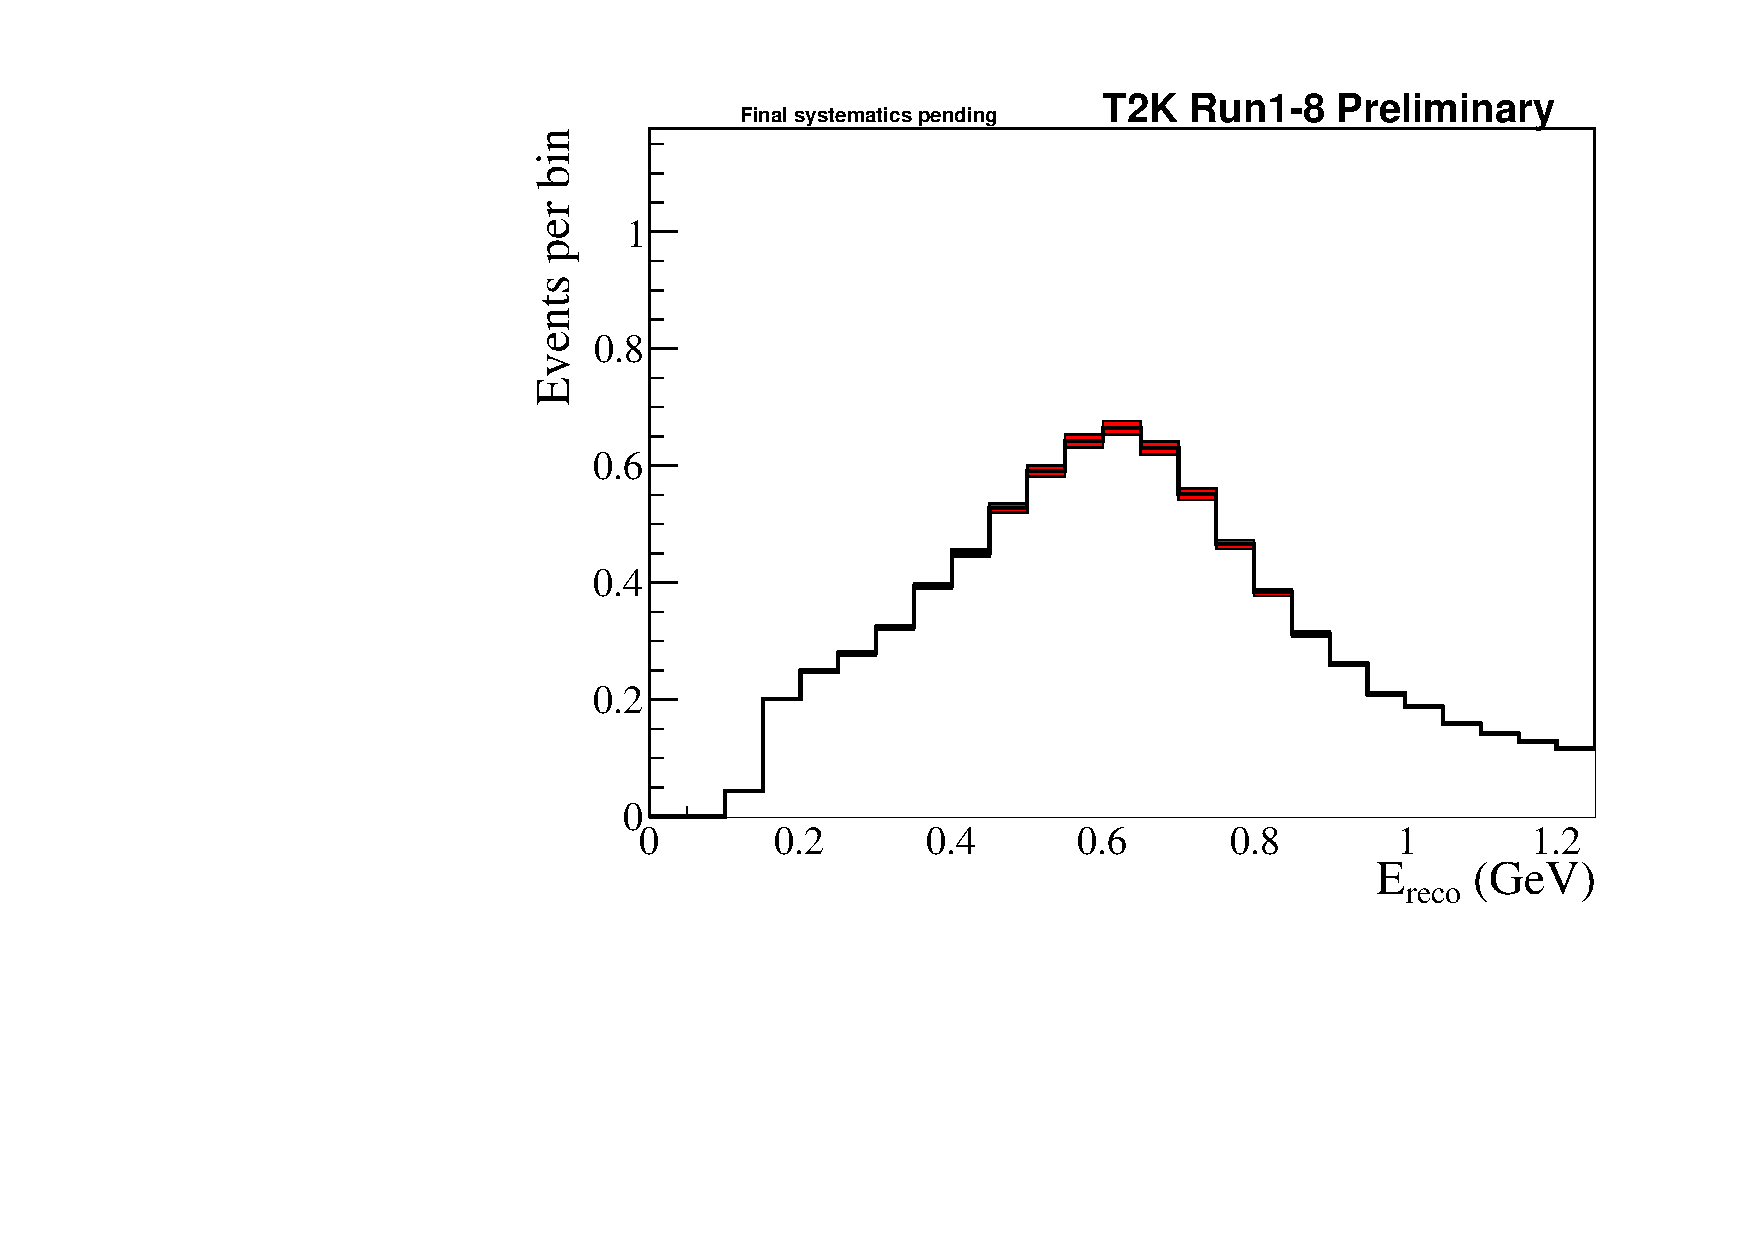
\includegraphics[width=0.9\textwidth]{systematics/envelopes/sk_errors/sk_error_table_RHC1Re_xsec_nue_envelope}
		\caption{Electron-like antineutrino mode}
	\end{subfigure}
	\begin{subfigure}[b]{0.49\textwidth}
		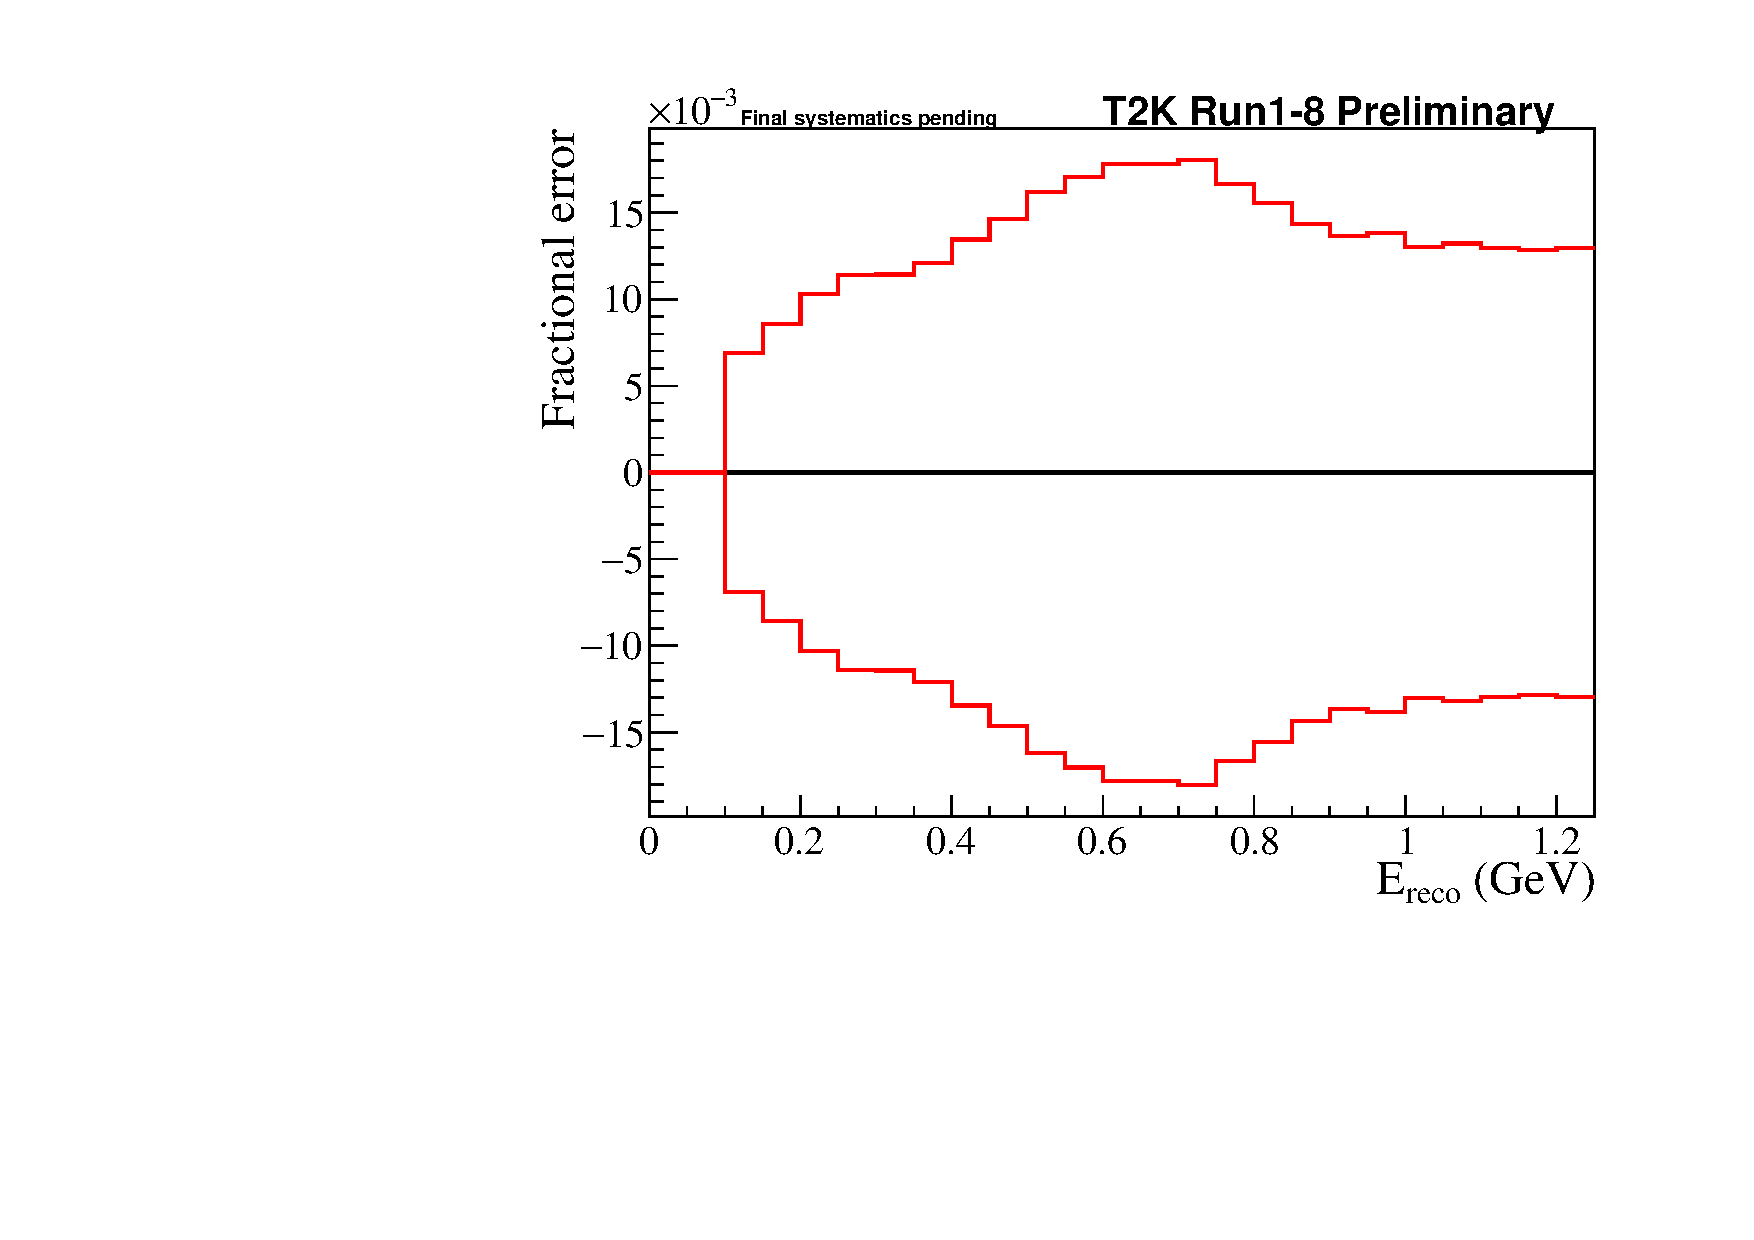
\includegraphics[width=0.9\textwidth]{systematics/envelopes/sk_errors/sk_error_table_RHC1Re_xsec_nue_envelope_fractional}
		\caption{Electron-like antineutrino mode}
	\end{subfigure}
	\caption {
		Error envelopes (left) and fractional errors (right) for the reconstructed neutrino energy spectrum for the unconstrained electron neutrino cross-section systematic parameters. \num{1e4} toys are generated for the Asimov data set A with randomized systematic parameters with correlations taken into account.
	}
	\label{fig:sk_envelopes_xsec_nue_b}
\end{figure*}
\clearpage
\begin{figure*}
	\center
	\begin{subfigure}[b]{0.49\textwidth}
		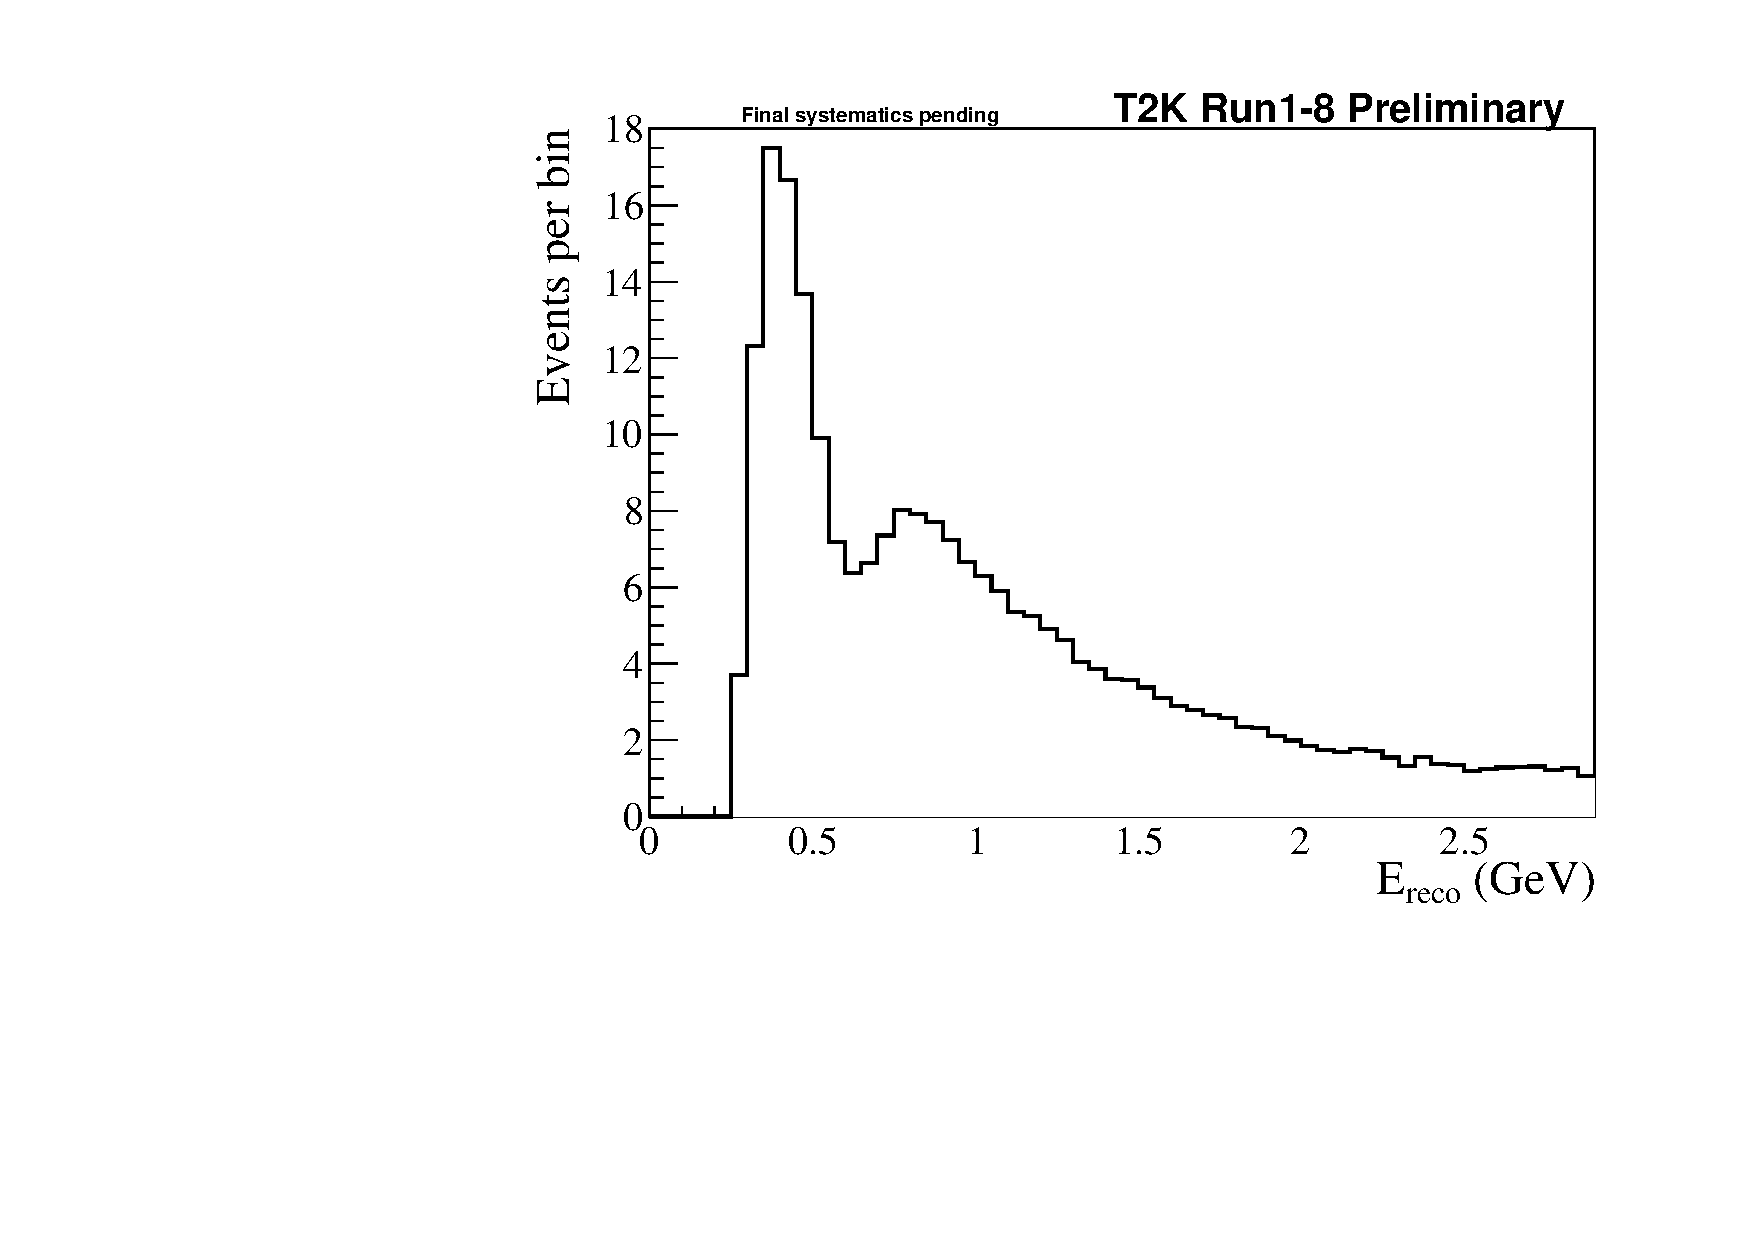
\includegraphics[width=0.9\textwidth]{systematics/envelopes/sk_errors/sk_error_table_1Rmu_xsec_ncgamma_envelope}
		\caption{Muon-like, neutrino mode}
	\end{subfigure}
	\begin{subfigure}[b]{0.49\textwidth}
		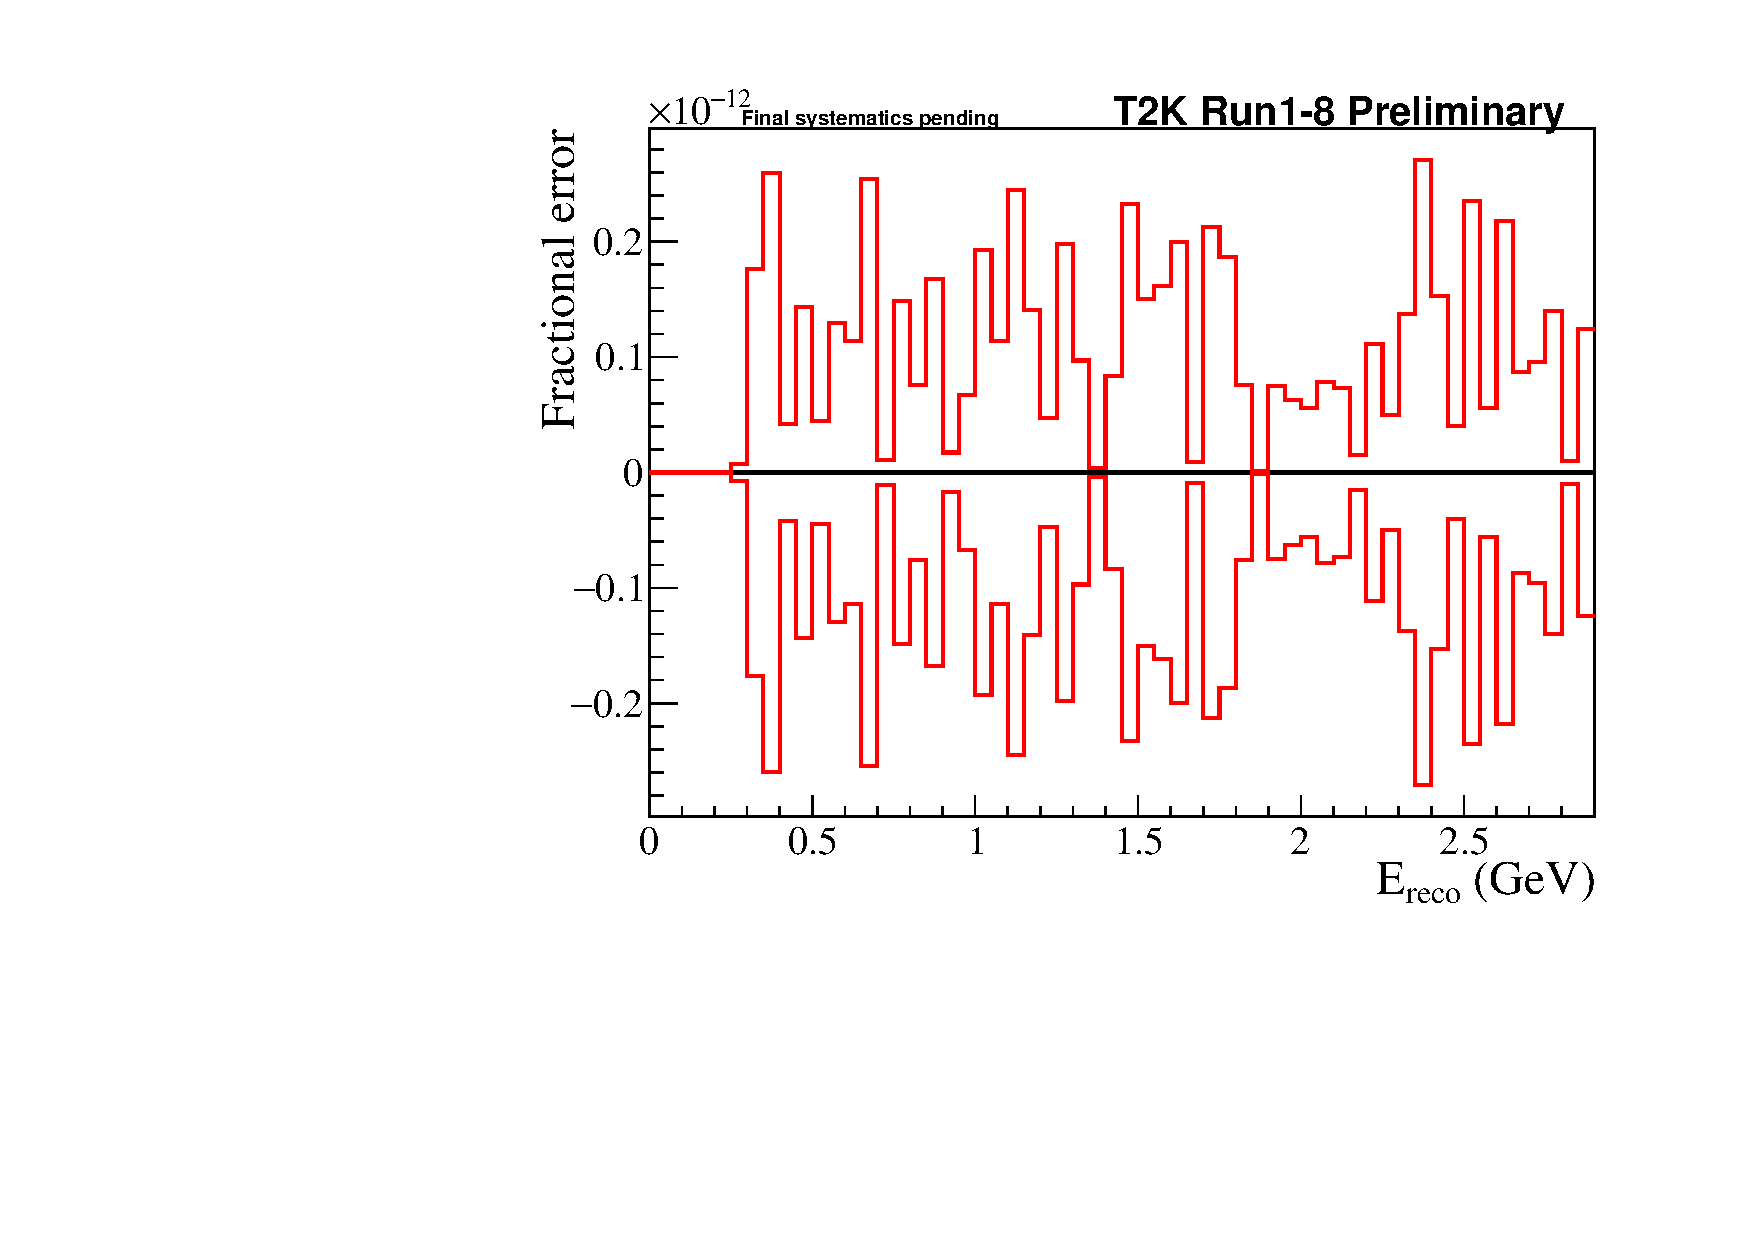
\includegraphics[width=0.9\textwidth]{systematics/envelopes/sk_errors/sk_error_table_1Rmu_xsec_ncgamma_envelope_fractional}
		\caption{Muon-like, neutrino mode}
	\end{subfigure}
	\begin{subfigure}[b]{0.49\textwidth}
		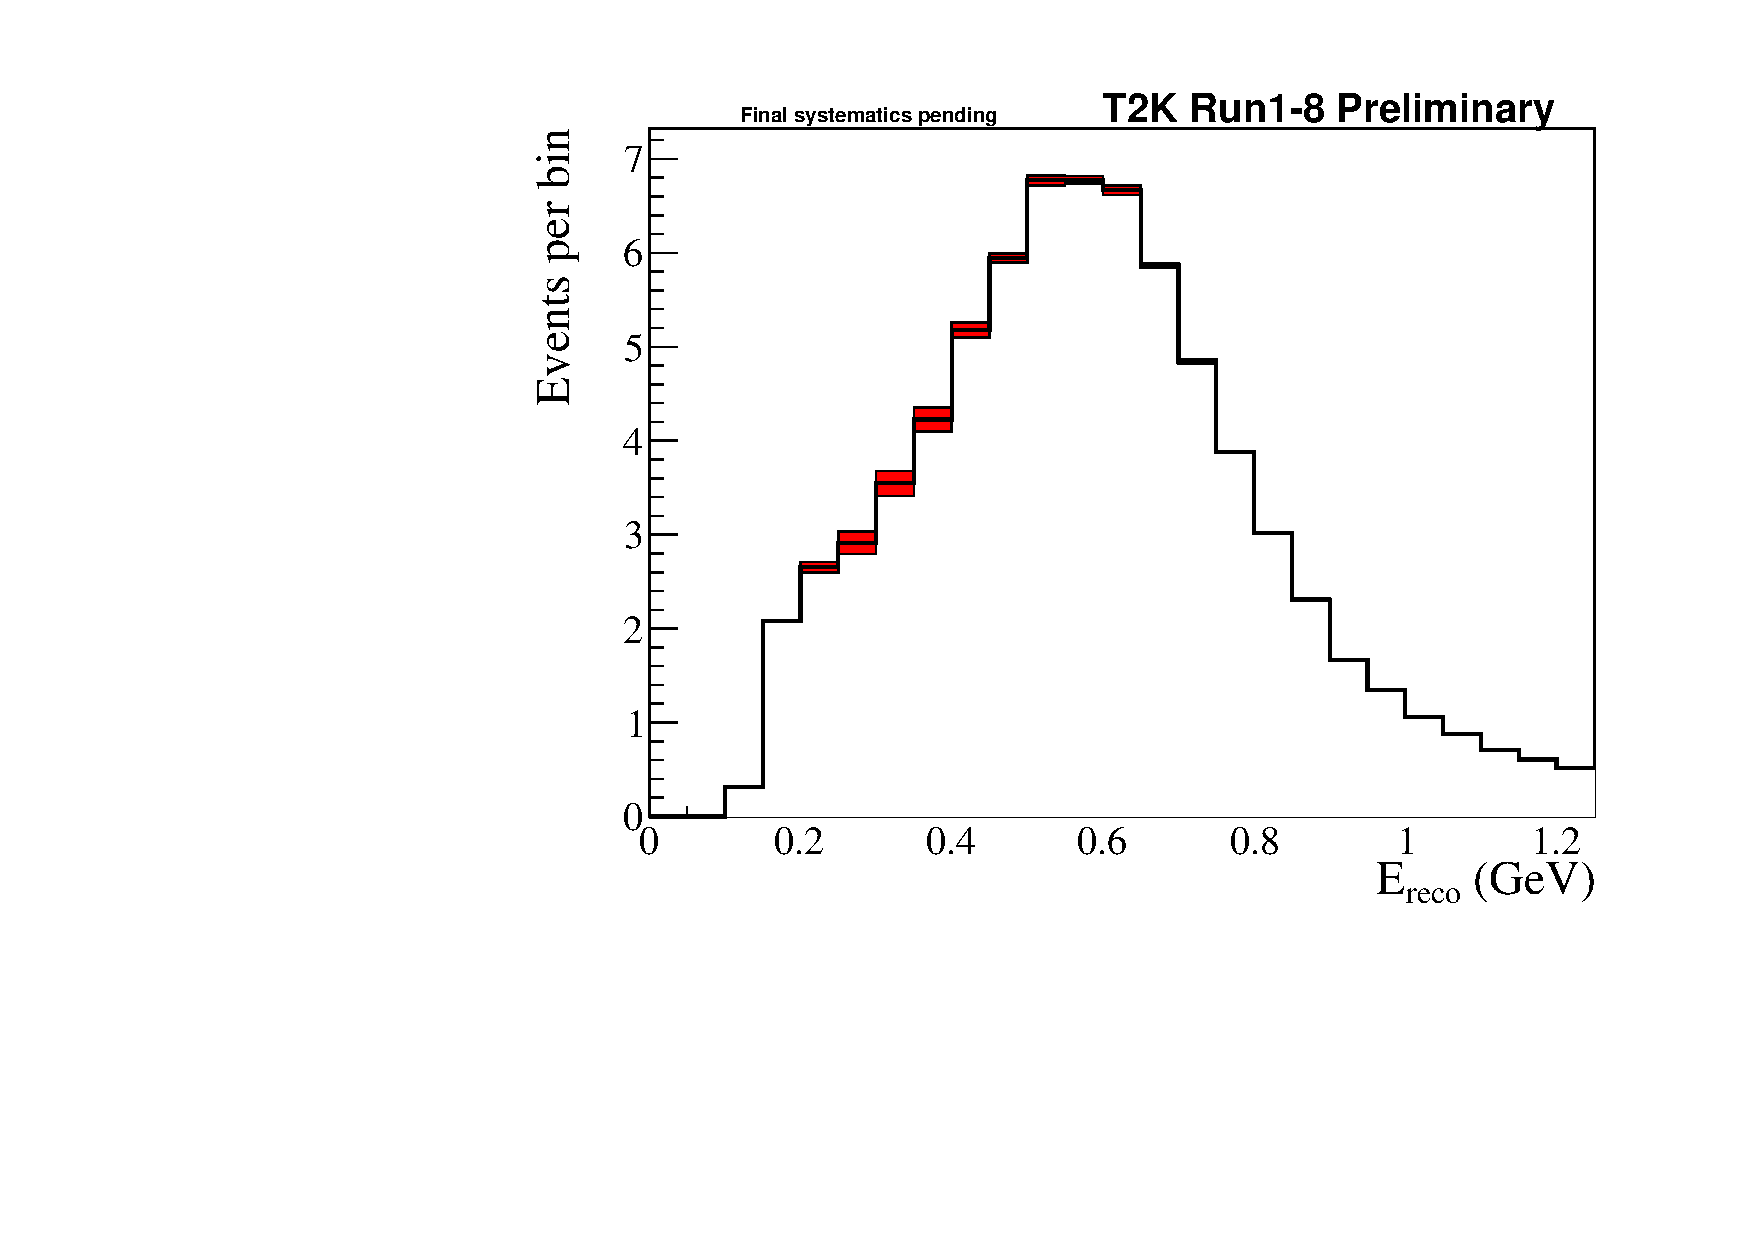
\includegraphics[width=0.9\textwidth]{systematics/envelopes/sk_errors/sk_error_table_1Re_xsec_ncgamma_envelope}
		\caption{Electron-like, neutrino mode}
	\end{subfigure}
	\begin{subfigure}[b]{0.49\textwidth}
		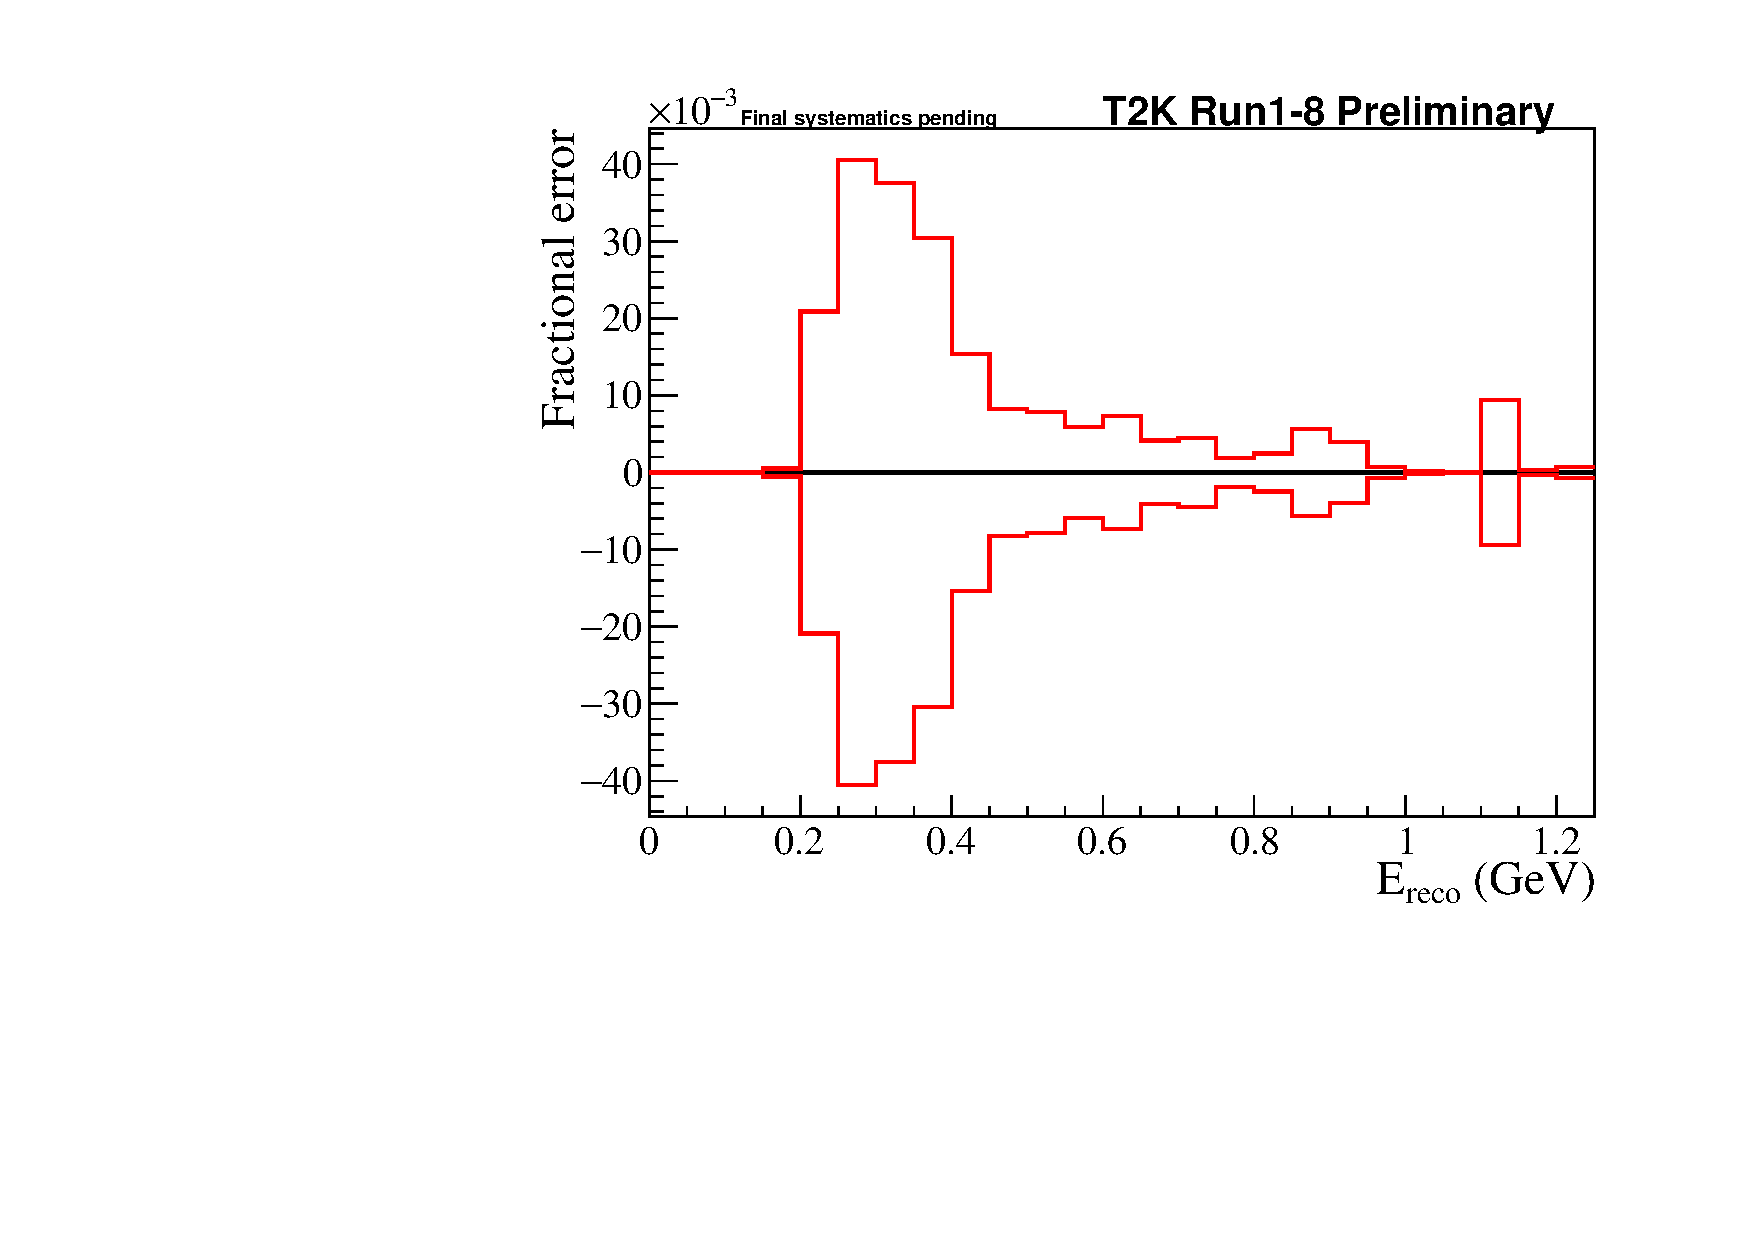
\includegraphics[width=0.9\textwidth]{systematics/envelopes/sk_errors/sk_error_table_1Re_xsec_ncgamma_envelope_fractional}
		\caption{Electron-like, neutrino mode}
	\end{subfigure}
	\begin{subfigure}[b]{0.49\textwidth}
		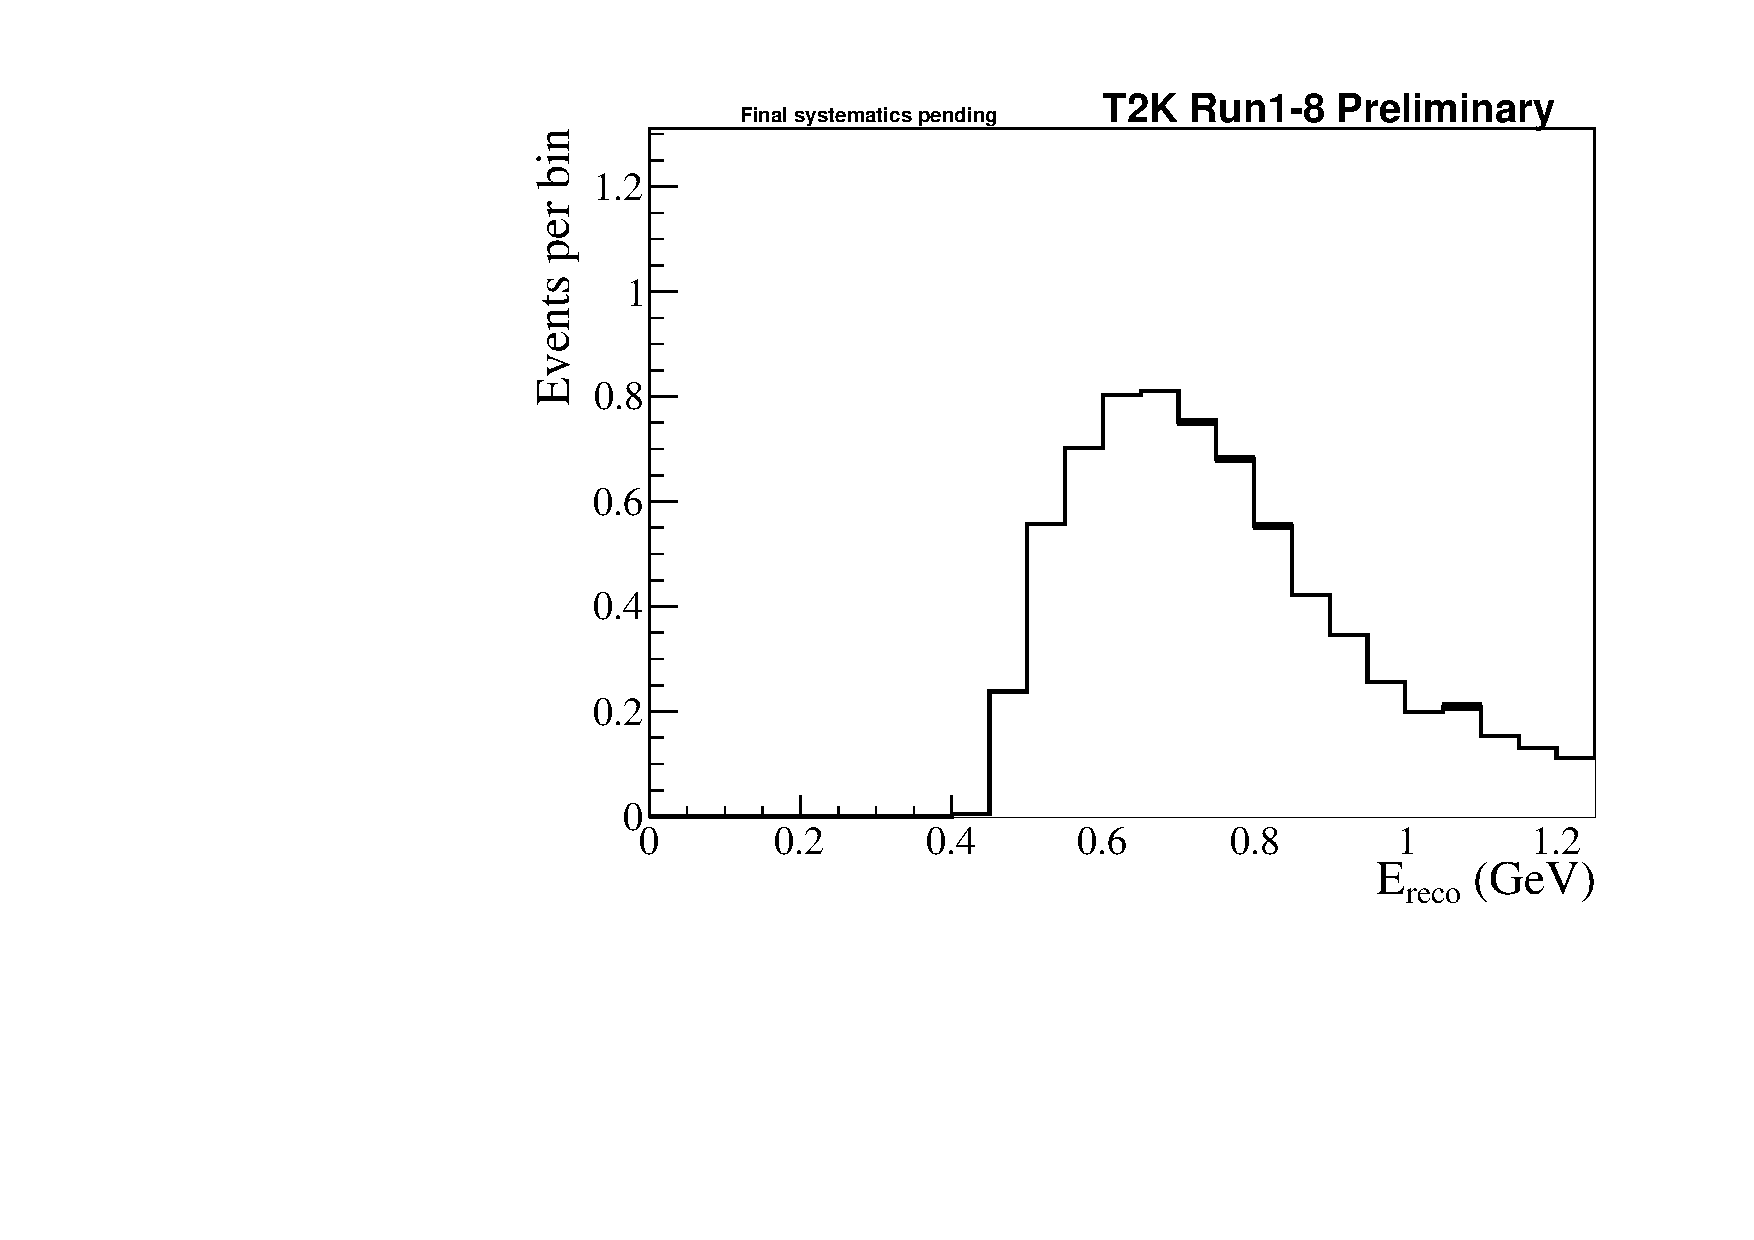
\includegraphics[width=0.9\textwidth]{systematics/envelopes/sk_errors/sk_error_table_MultiRe_xsec_ncgamma_envelope}
		\caption{\nueCConepi-like, neutrino mode}
	\end{subfigure}
	\begin{subfigure}[b]{0.49\textwidth}
		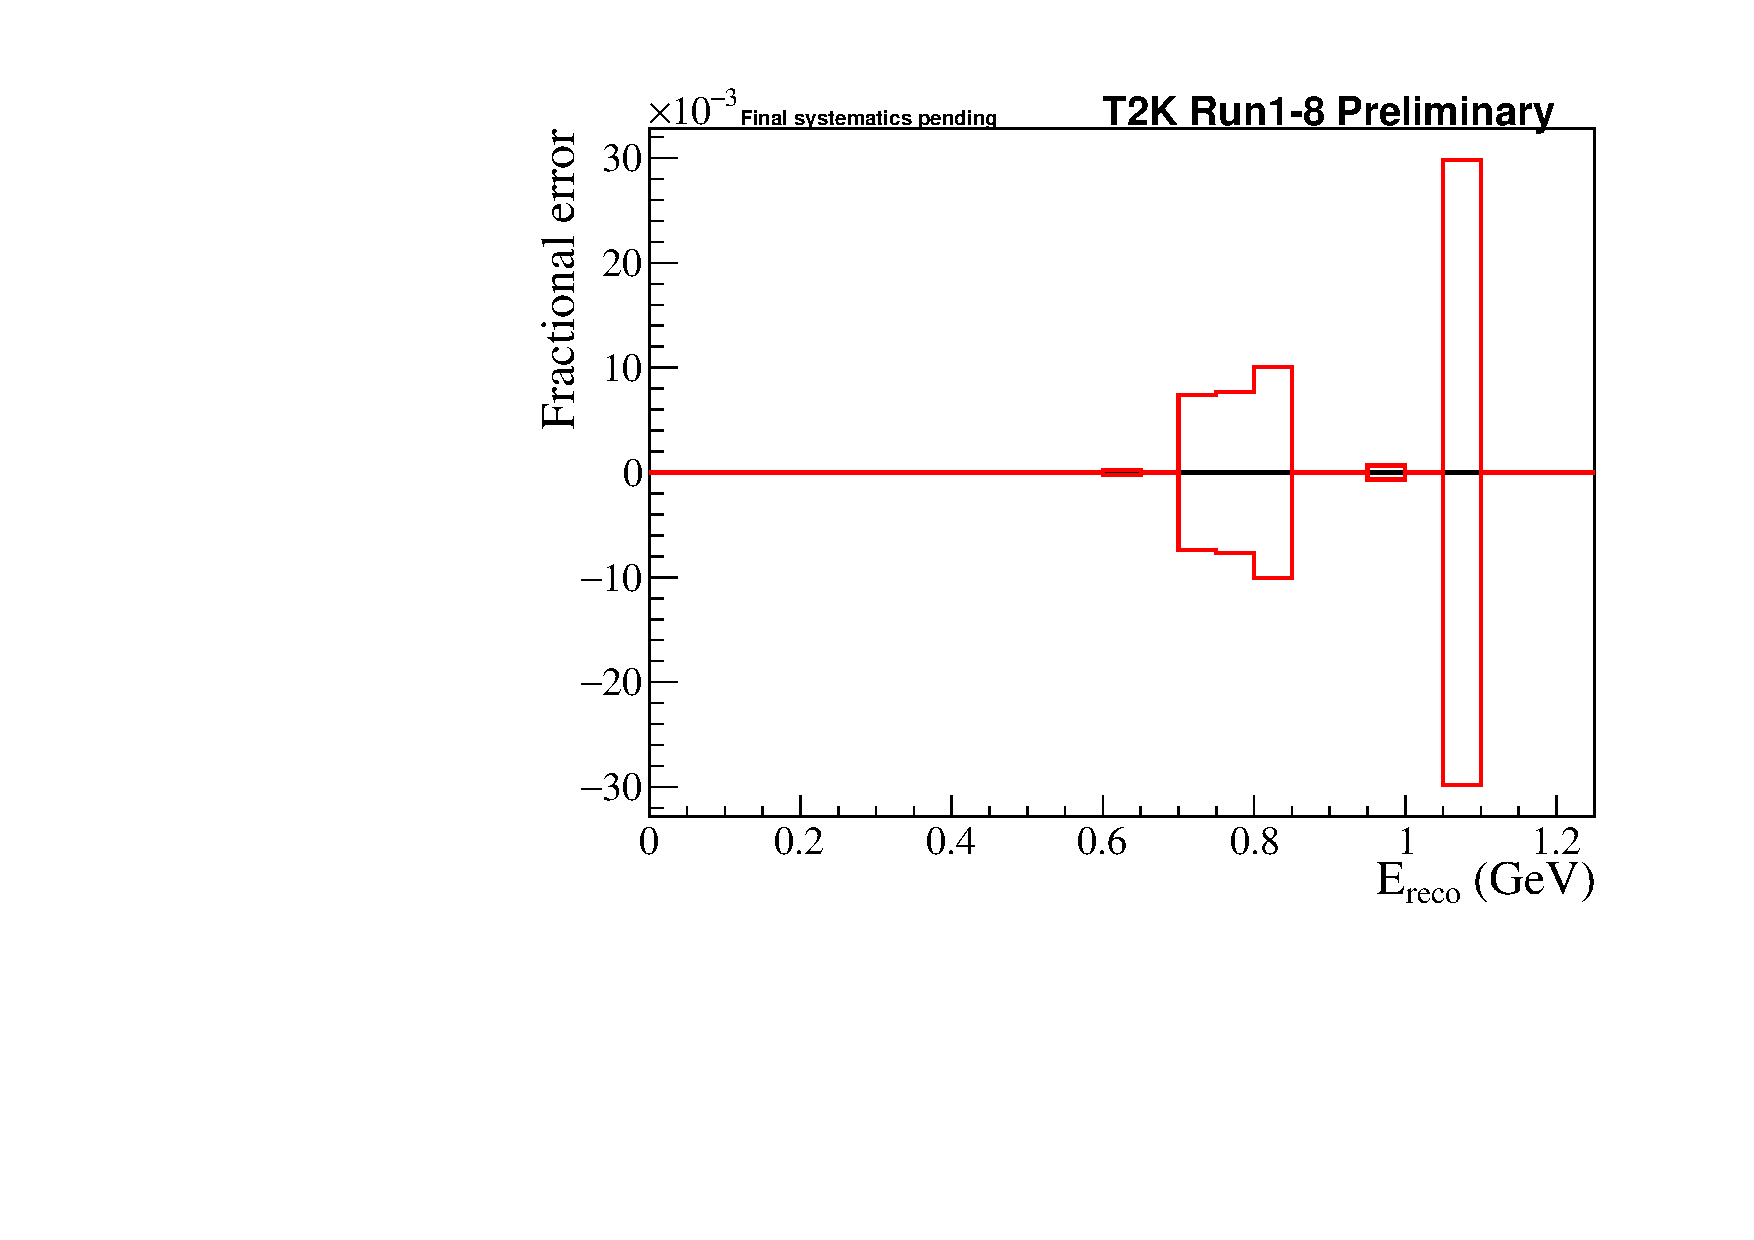
\includegraphics[width=0.9\textwidth]{systematics/envelopes/sk_errors/sk_error_table_MultiRe_xsec_ncgamma_envelope_fractional}
		\caption{\nueCConepi-like, neutrino mode}
	\end{subfigure}
	\caption {
		Error envelopes (left) and fractional error (right) for the reconstructed neutrino energy spectrum for the unconstrained NC$1\gamma$ systematic parameters. \num{1e4} toys are generated for the Asimov data set A with randomized systematic parameters with correlations taken into account.
	}
	\label{fig:sk_envelopes_xsec_ncgamma}
\end{figure*}
\clearpage

\begin{figure*}
	\center
	\begin{subfigure}[b]{0.49\textwidth}
		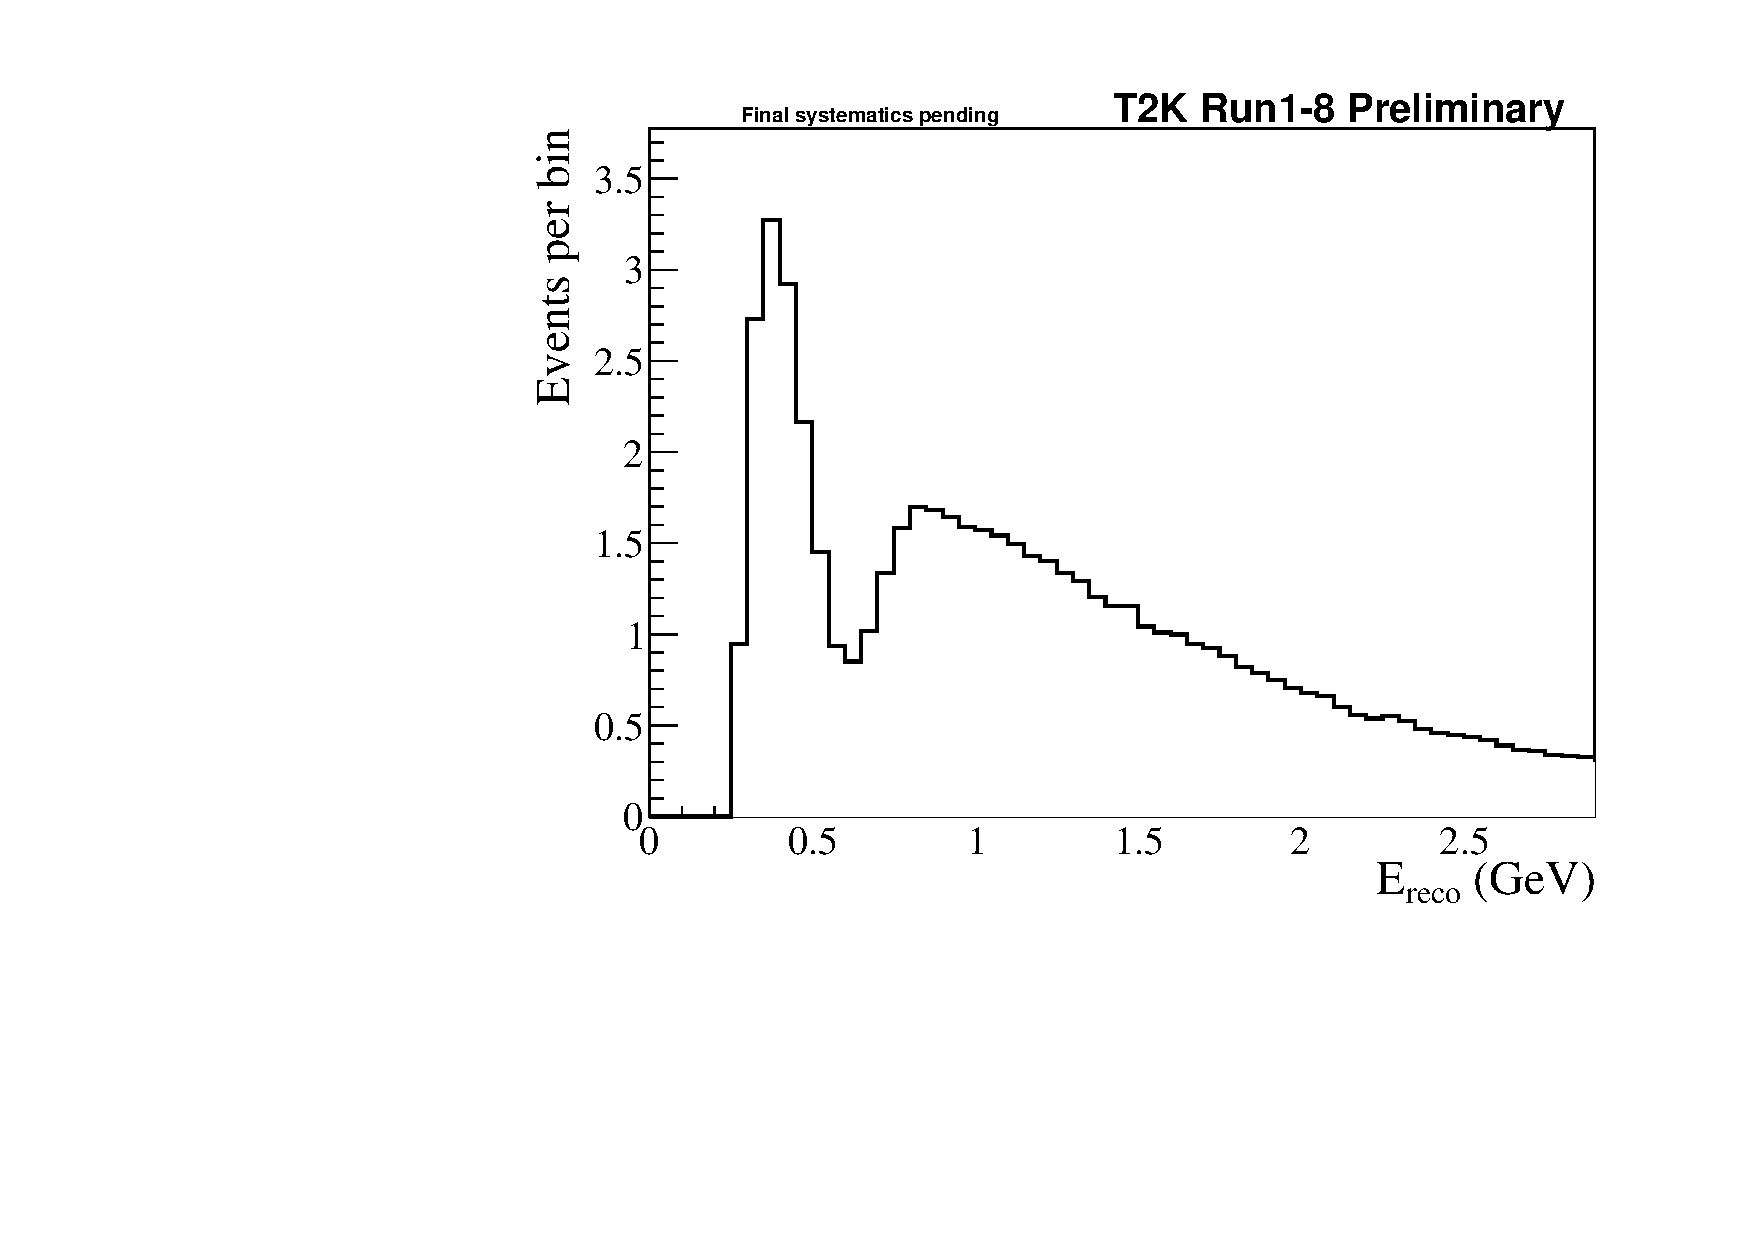
\includegraphics[width=0.9\textwidth]{systematics/envelopes/sk_errors/sk_error_table_RHC1Rmu_xsec_ncgamma_envelope}
		\caption{Muon-like, antineutrino mode}
	\end{subfigure}
	\begin{subfigure}[b]{0.49\textwidth}
		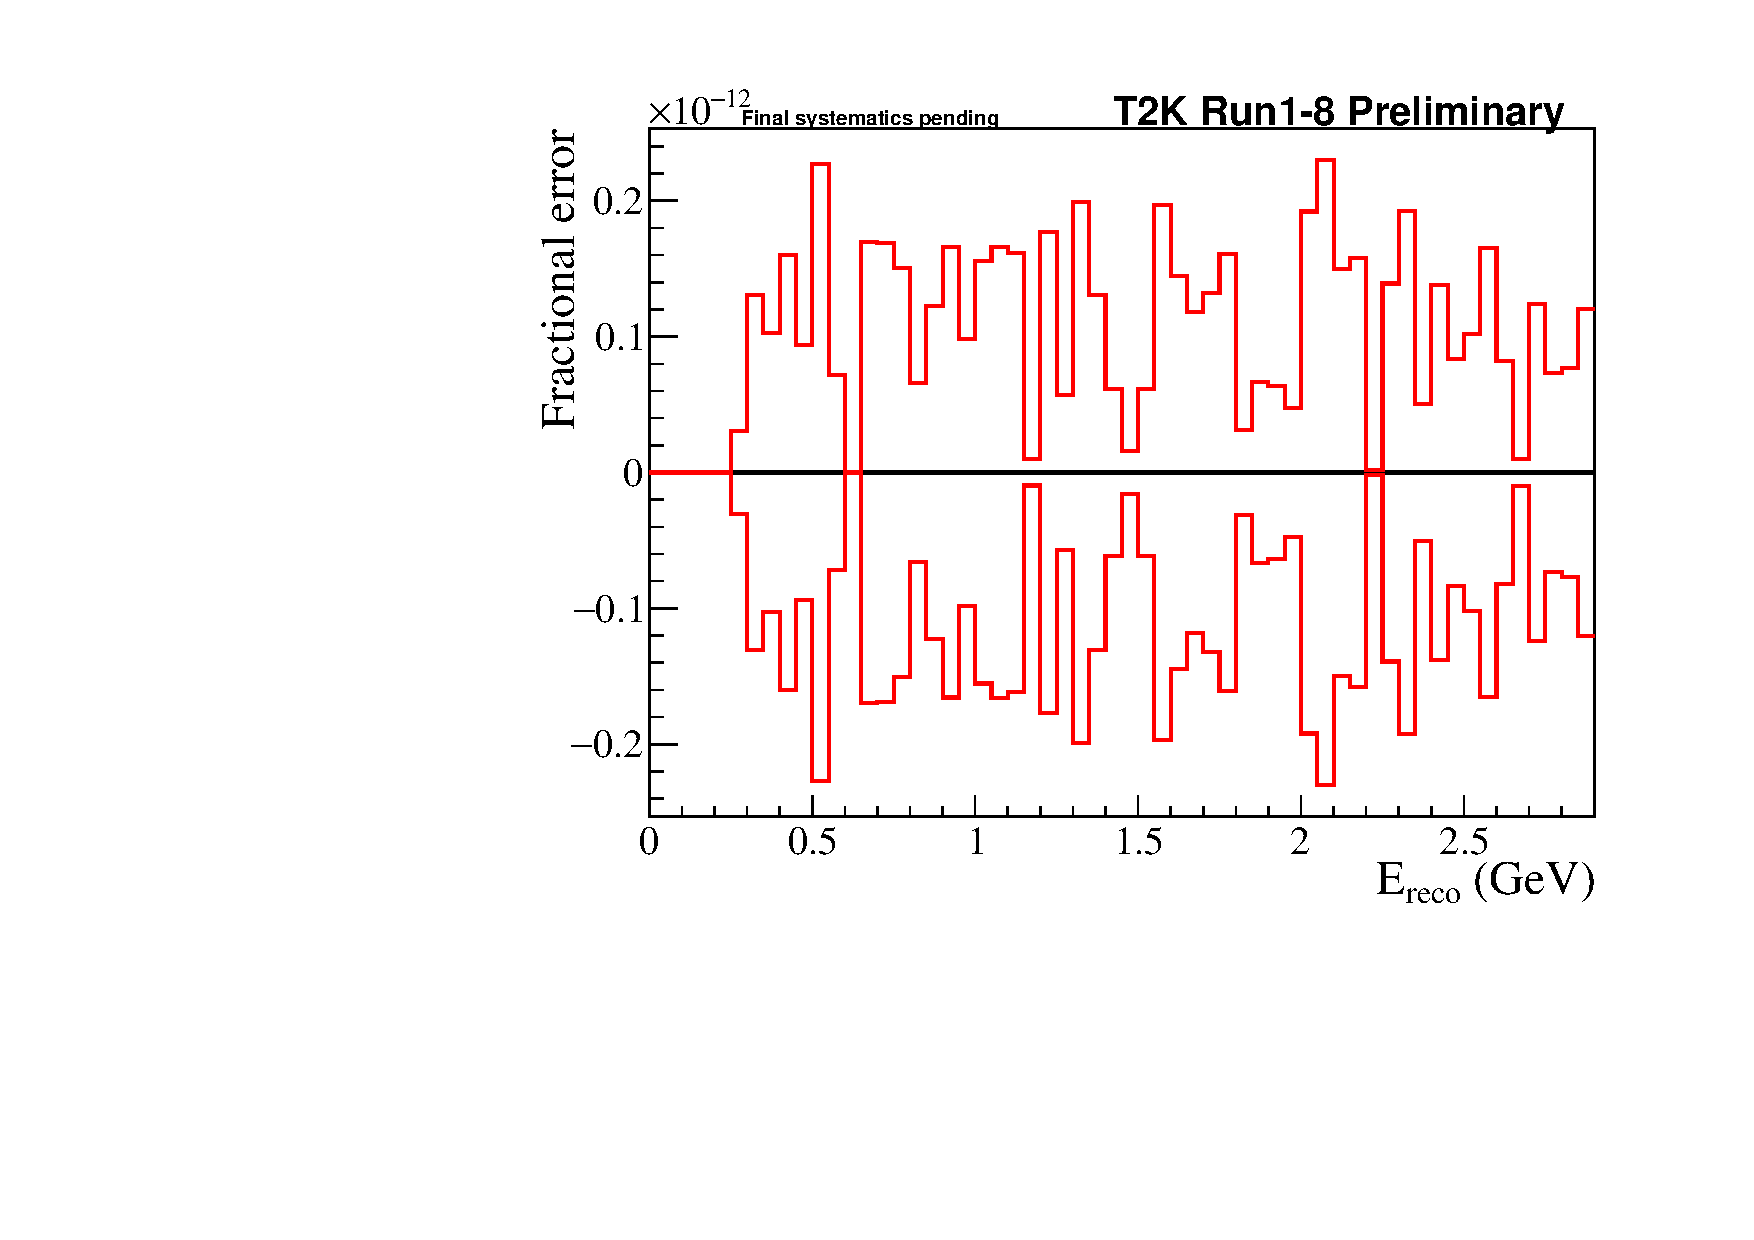
\includegraphics[width=0.9\textwidth]{systematics/envelopes/sk_errors/sk_error_table_RHC1Rmu_xsec_ncgamma_envelope_fractional}
		\caption{Muon-like, antineutrino mode}
	\end{subfigure}
	\begin{subfigure}[b]{0.49\textwidth}
		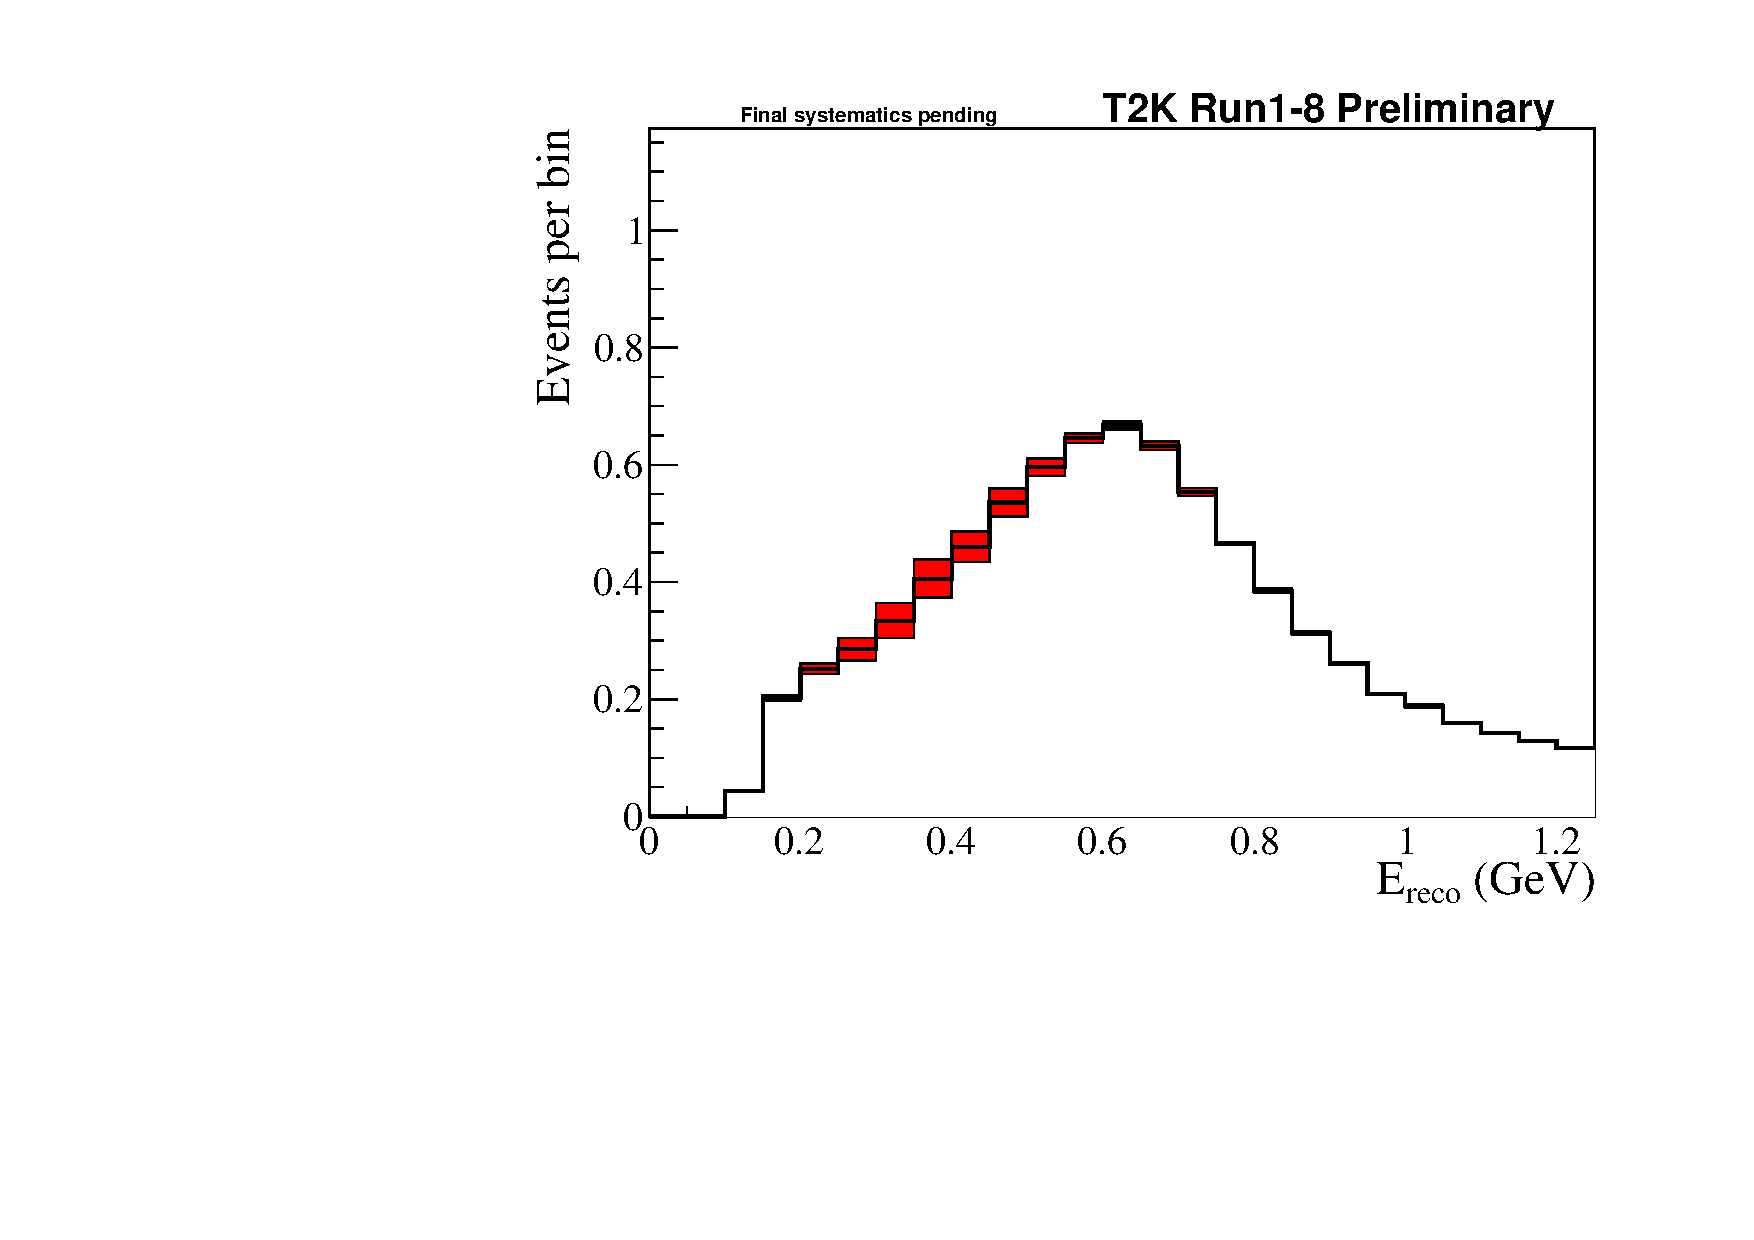
\includegraphics[width=0.9\textwidth]{systematics/envelopes/sk_errors/sk_error_table_RHC1Re_xsec_ncgamma_envelope}
		\caption{Electron-like antineutrino mode}
	\end{subfigure}
	\begin{subfigure}[b]{0.49\textwidth}
		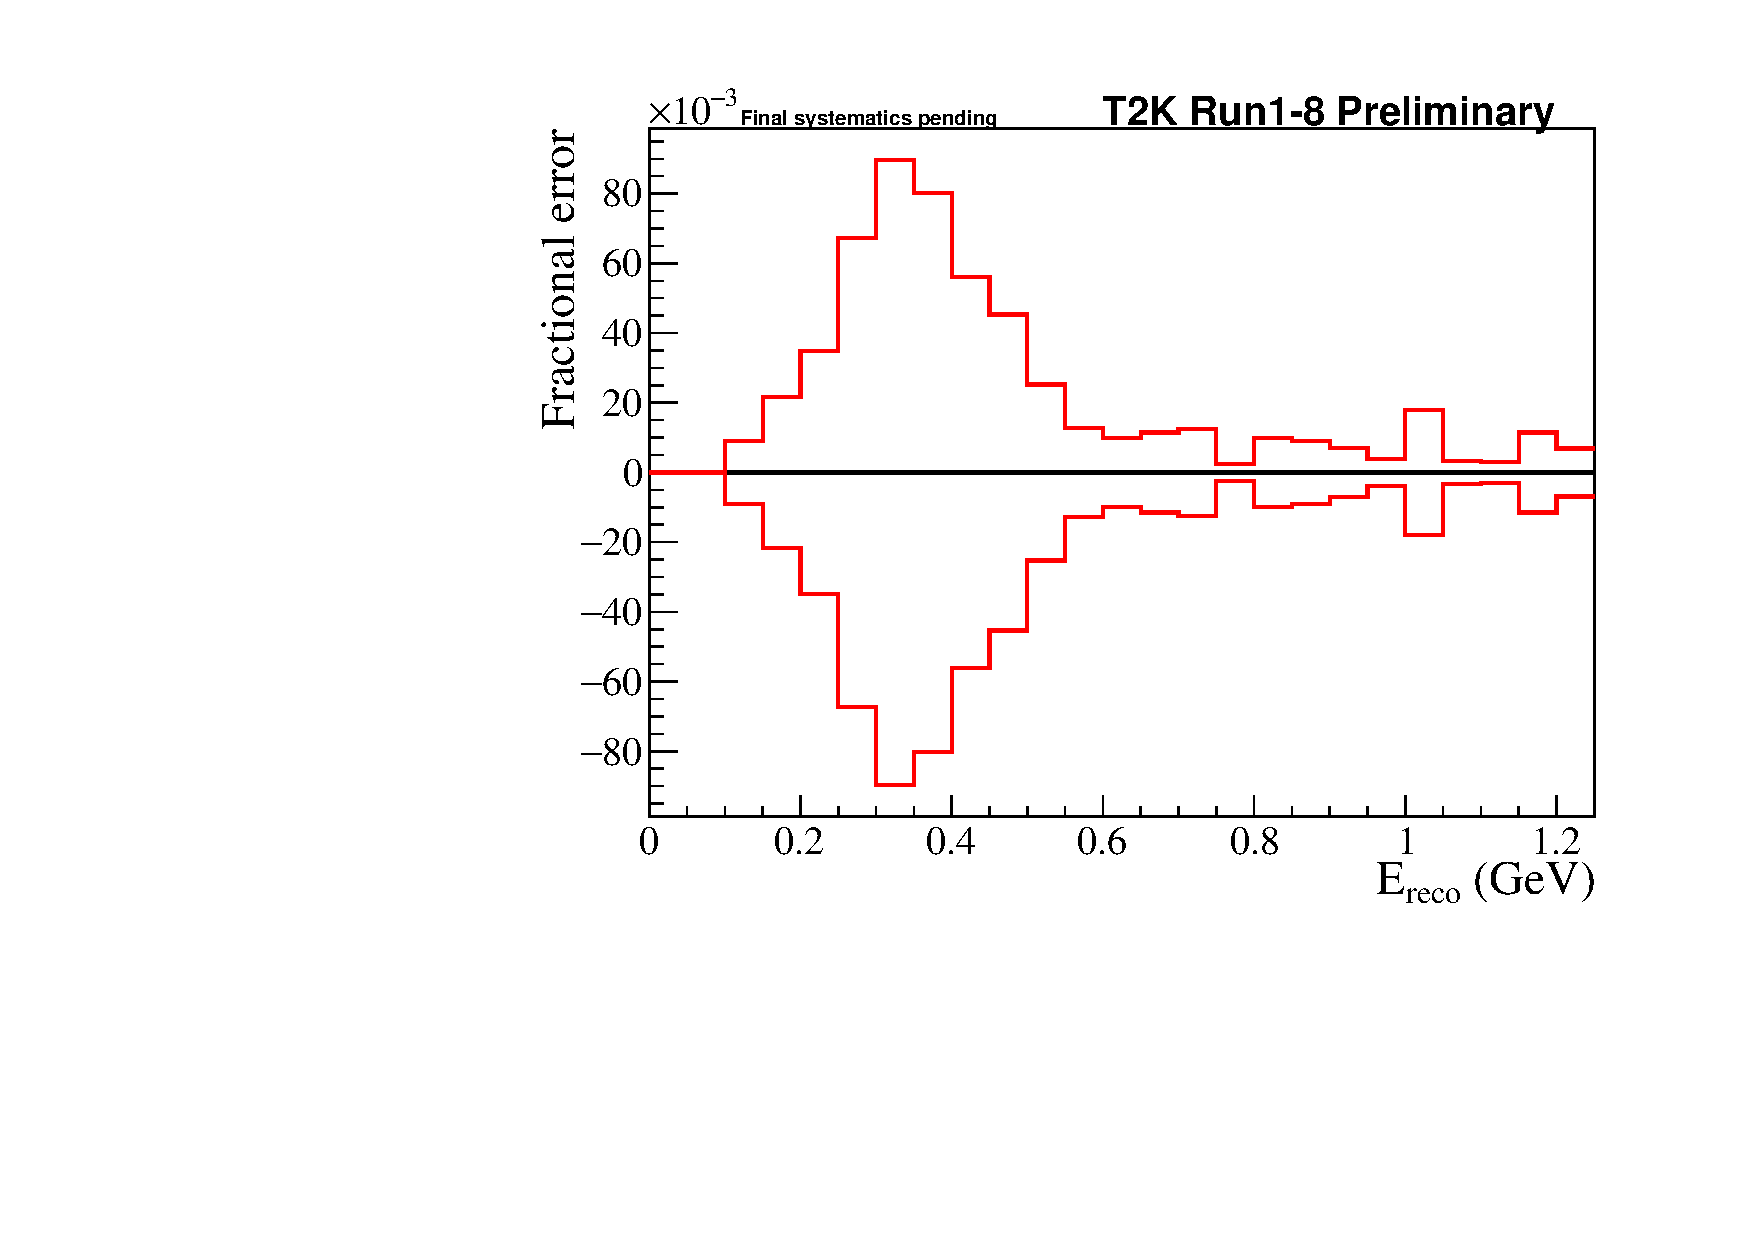
\includegraphics[width=0.9\textwidth]{systematics/envelopes/sk_errors/sk_error_table_RHC1Re_xsec_ncgamma_envelope_fractional}
		\caption{Electron-like antineutrino mode}
	\end{subfigure}
	\caption {
		Error envelopes (left) and fractional errors (right) for the reconstructed neutrino energy spectrum for the unconstrained NC$1\gamma$ systematic parameters. \num{1e4} toys are generated for the Asimov data set A with randomized systematic parameters with correlations taken into account.
	}
	\label{fig:sk_envelopes_xsec_ncgamma_b}
\end{figure*}
\clearpage
\begin{figure*}
	\center
	\begin{subfigure}[b]{0.49\textwidth}
		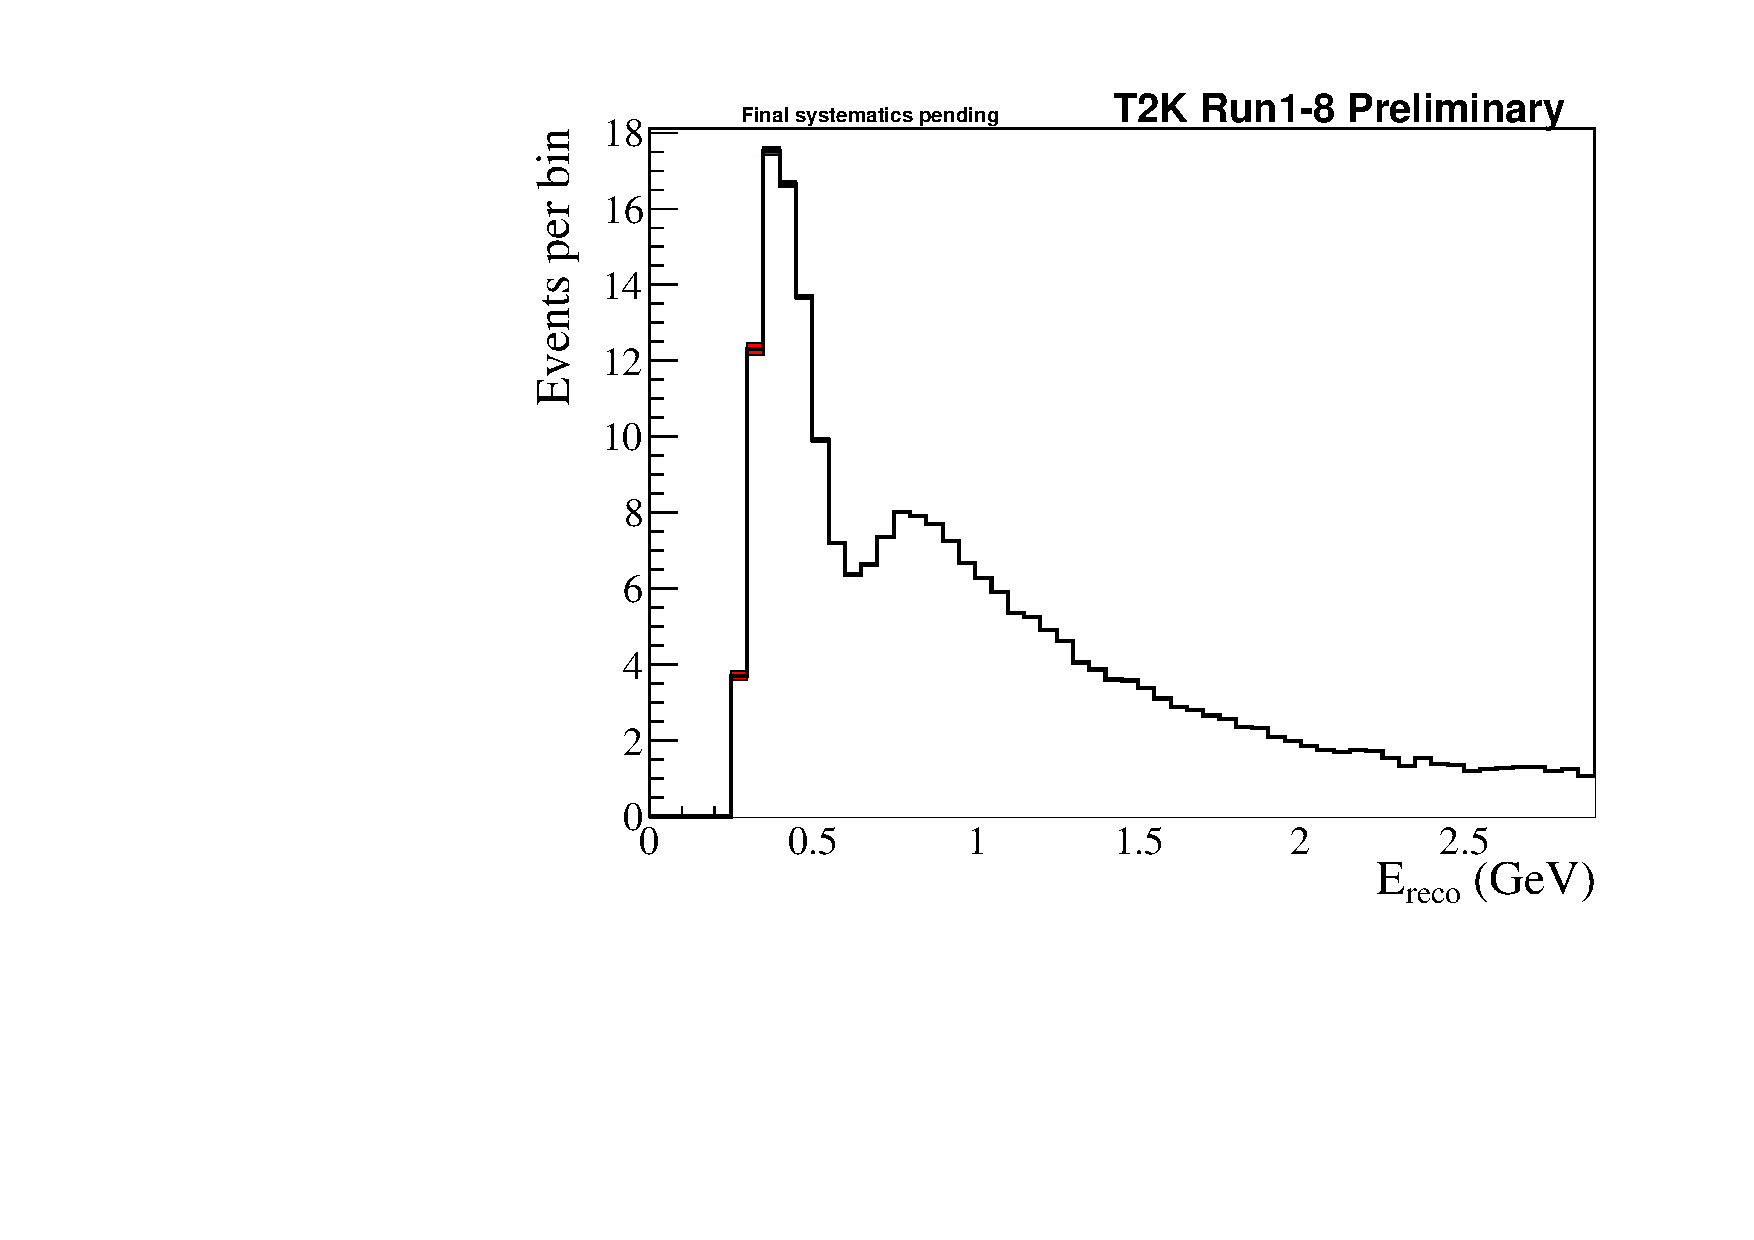
\includegraphics[width=0.9\textwidth]{systematics/envelopes/sk_errors/sk_error_table_1Rmu_xsec_ncoth_envelope}
		\caption{Muon-like, neutrino mode}
	\end{subfigure}
	\begin{subfigure}[b]{0.49\textwidth}
		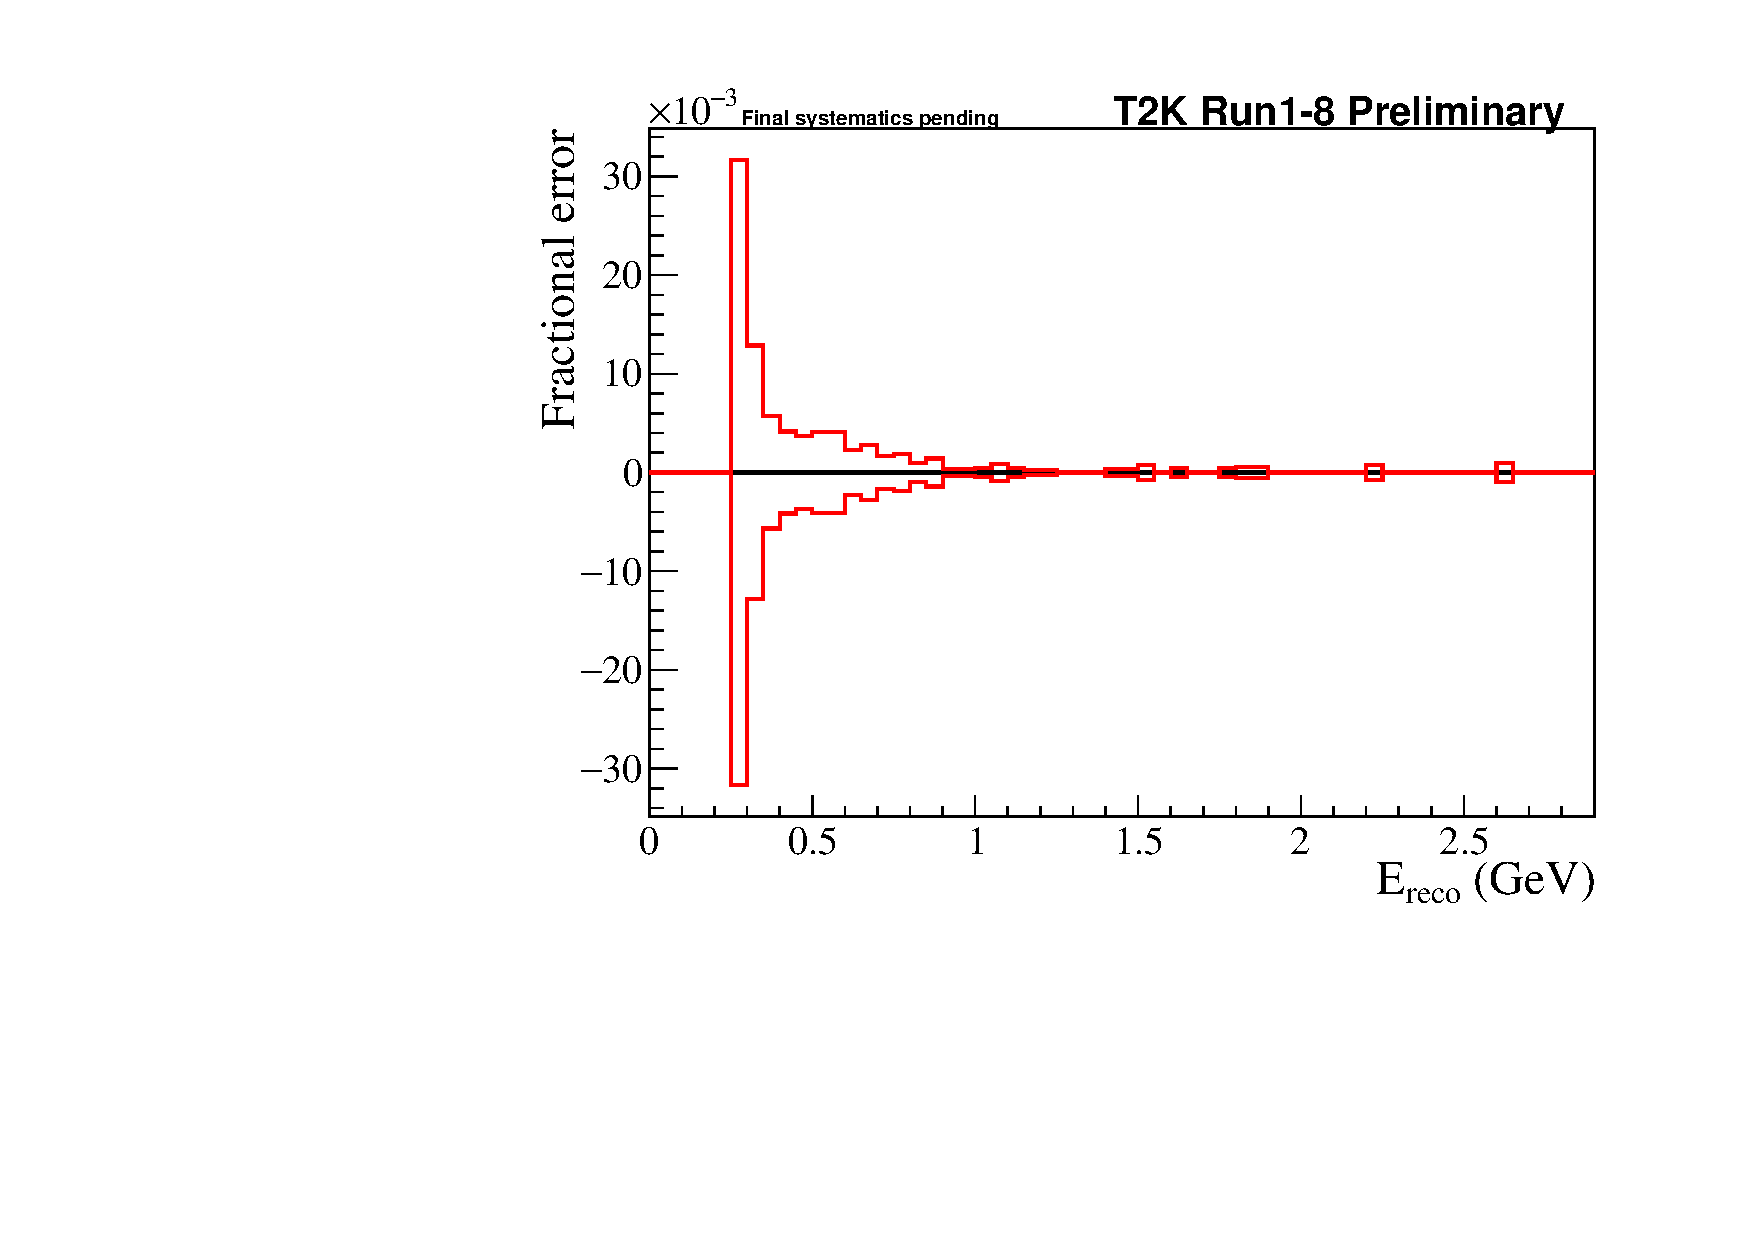
\includegraphics[width=0.9\textwidth]{systematics/envelopes/sk_errors/sk_error_table_1Rmu_xsec_ncoth_envelope_fractional}
		\caption{Muon-like, neutrino mode}
	\end{subfigure}
	\begin{subfigure}[b]{0.49\textwidth}
		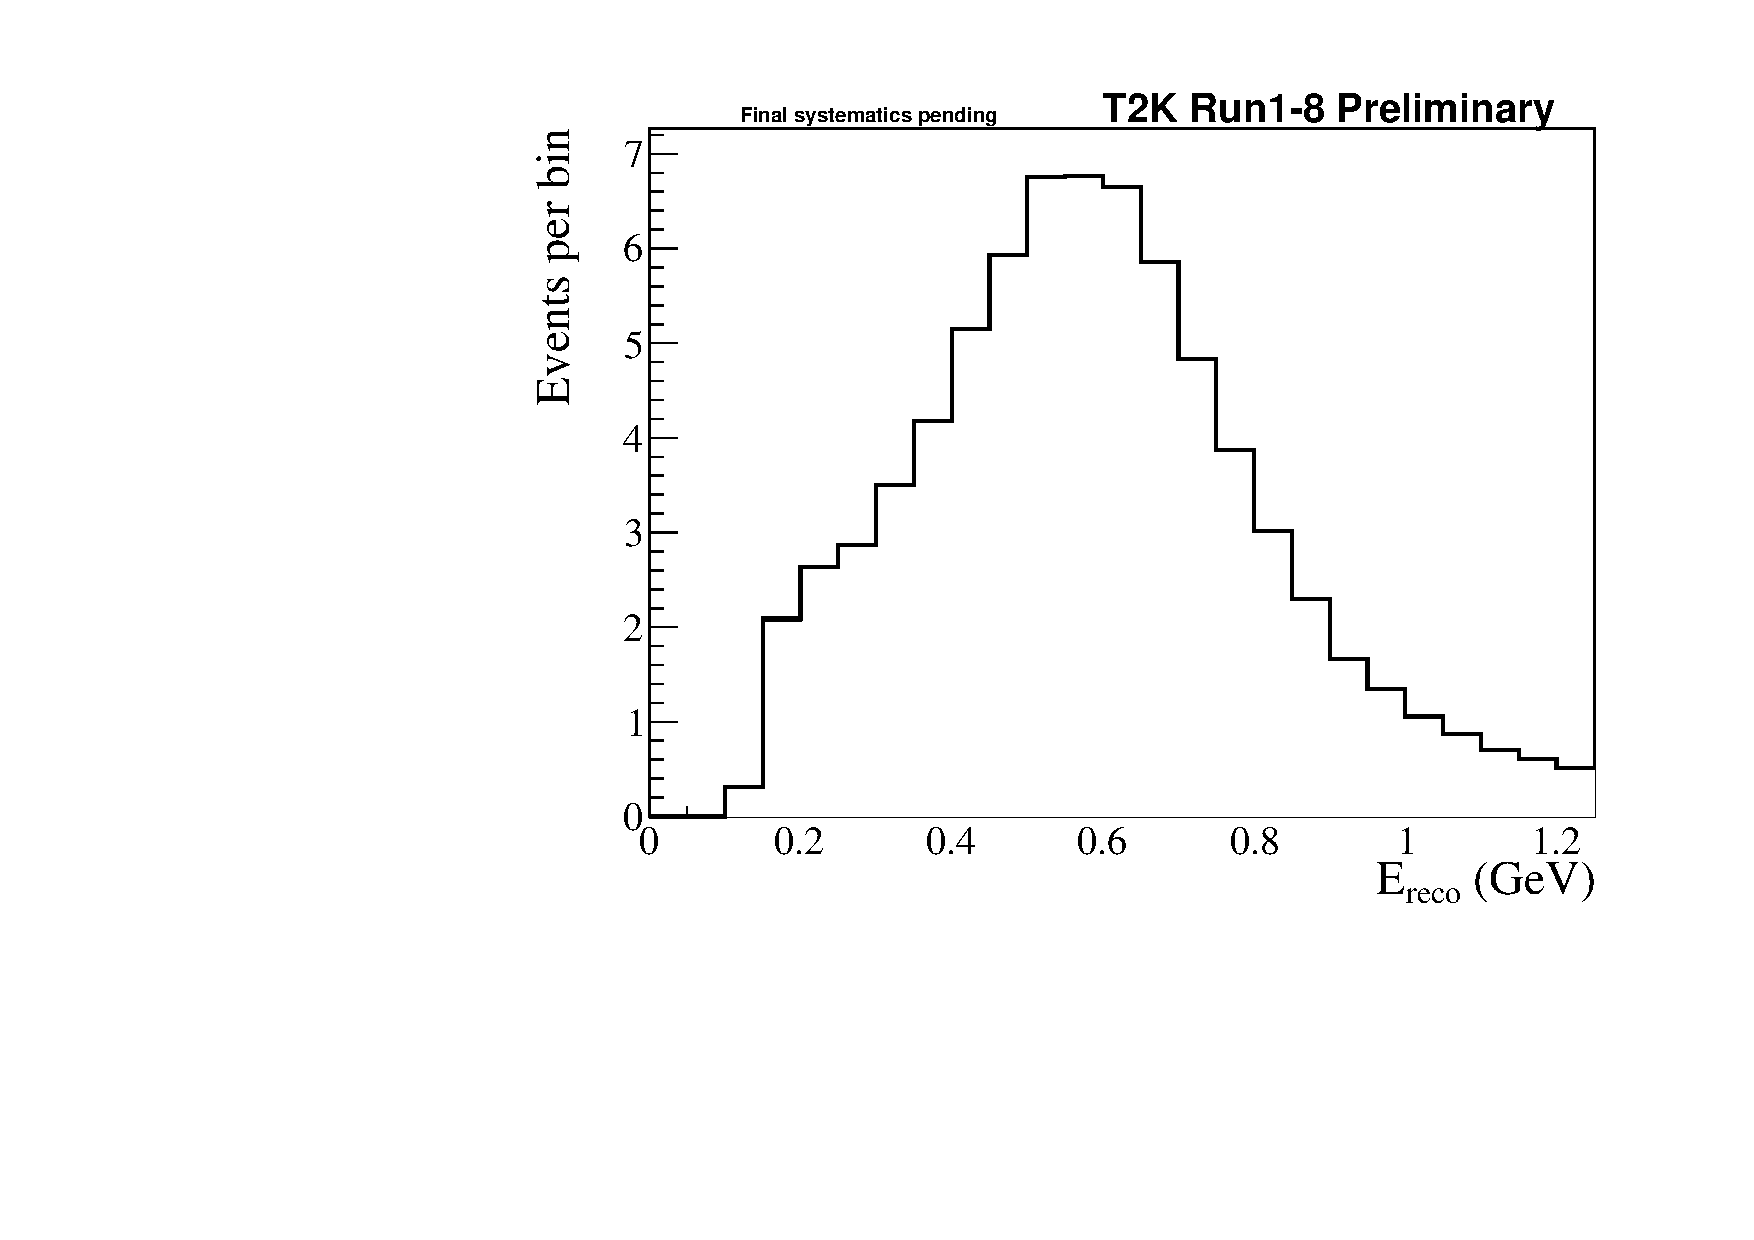
\includegraphics[width=0.9\textwidth]{systematics/envelopes/sk_errors/sk_error_table_1Re_xsec_ncoth_envelope}
		\caption{Electron-like, neutrino mode}
	\end{subfigure}
	\begin{subfigure}[b]{0.49\textwidth}
		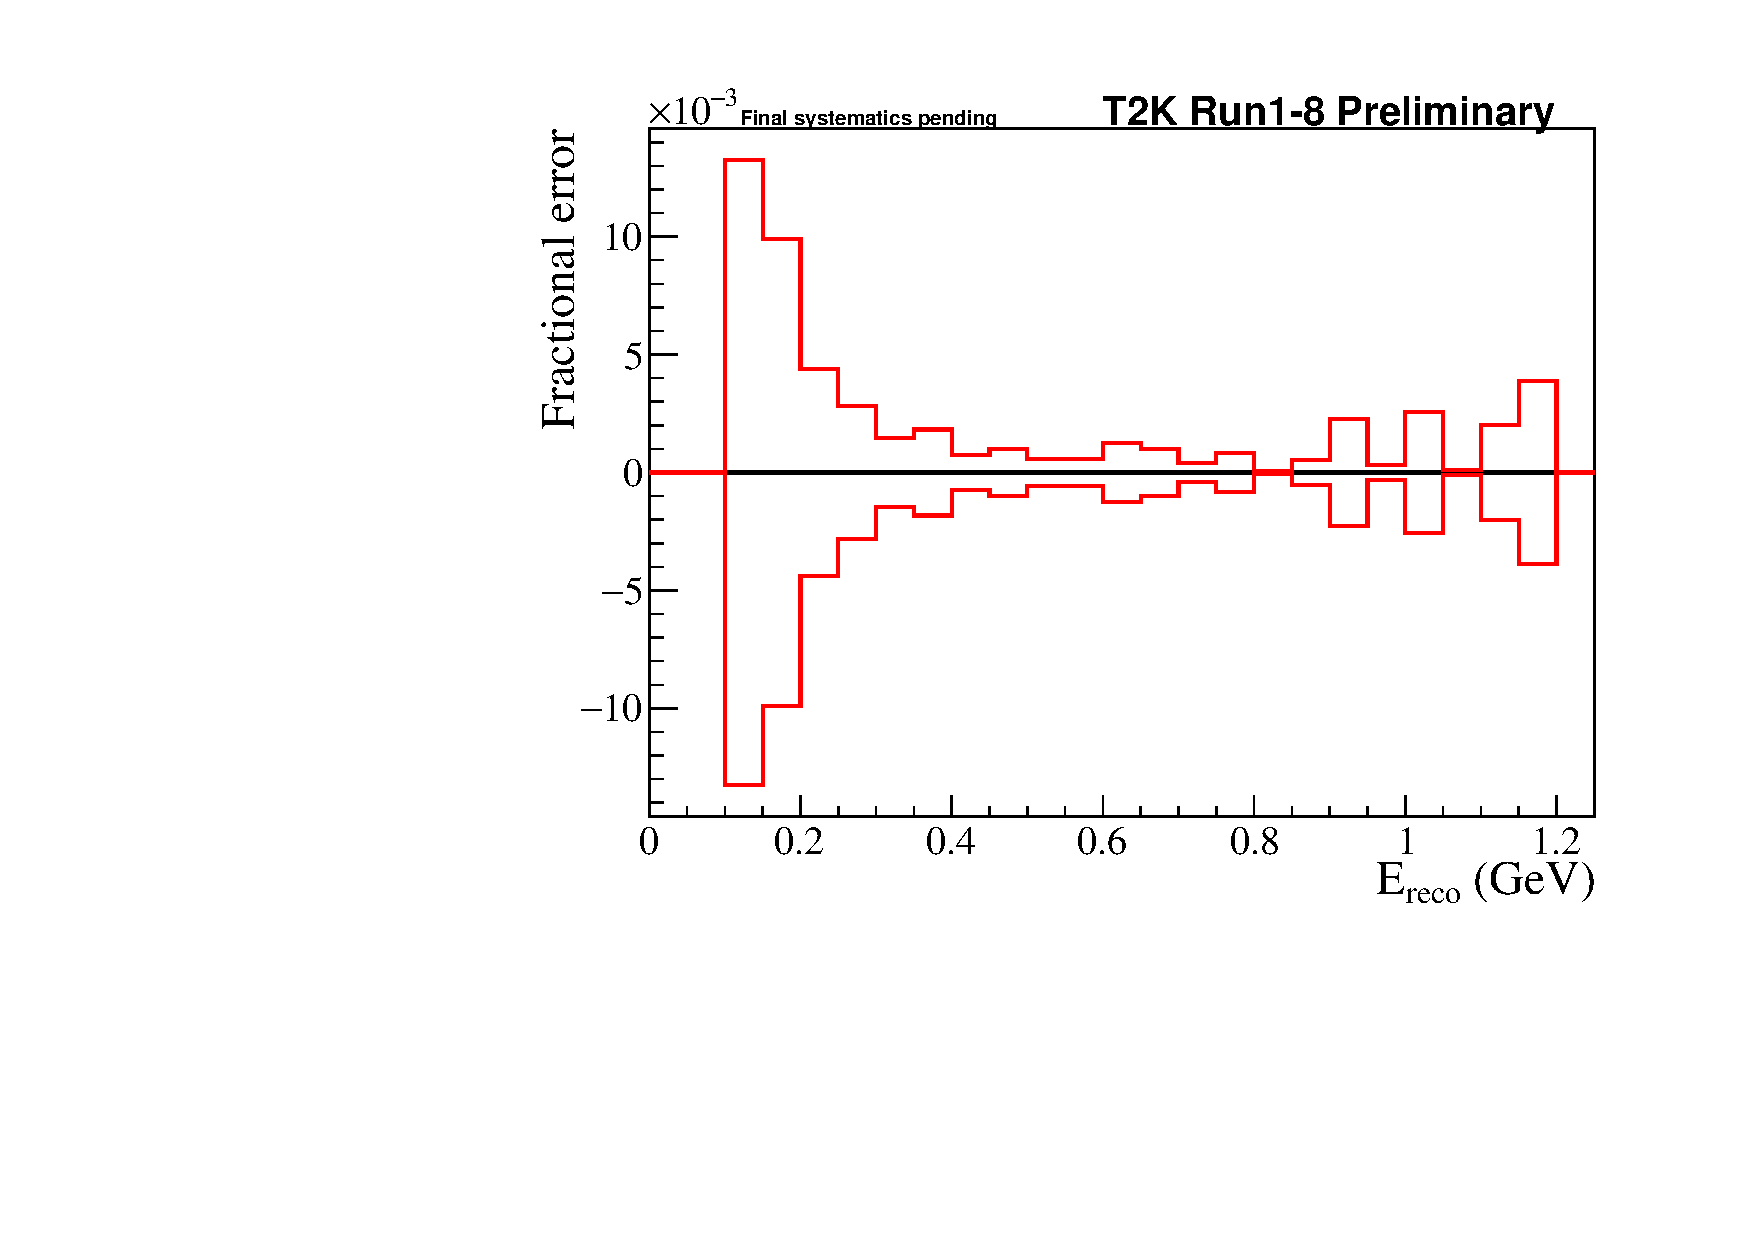
\includegraphics[width=0.9\textwidth]{systematics/envelopes/sk_errors/sk_error_table_1Re_xsec_ncoth_envelope_fractional}
		\caption{Electron-like, neutrino mode}
	\end{subfigure}
	\begin{subfigure}[b]{0.49\textwidth}
		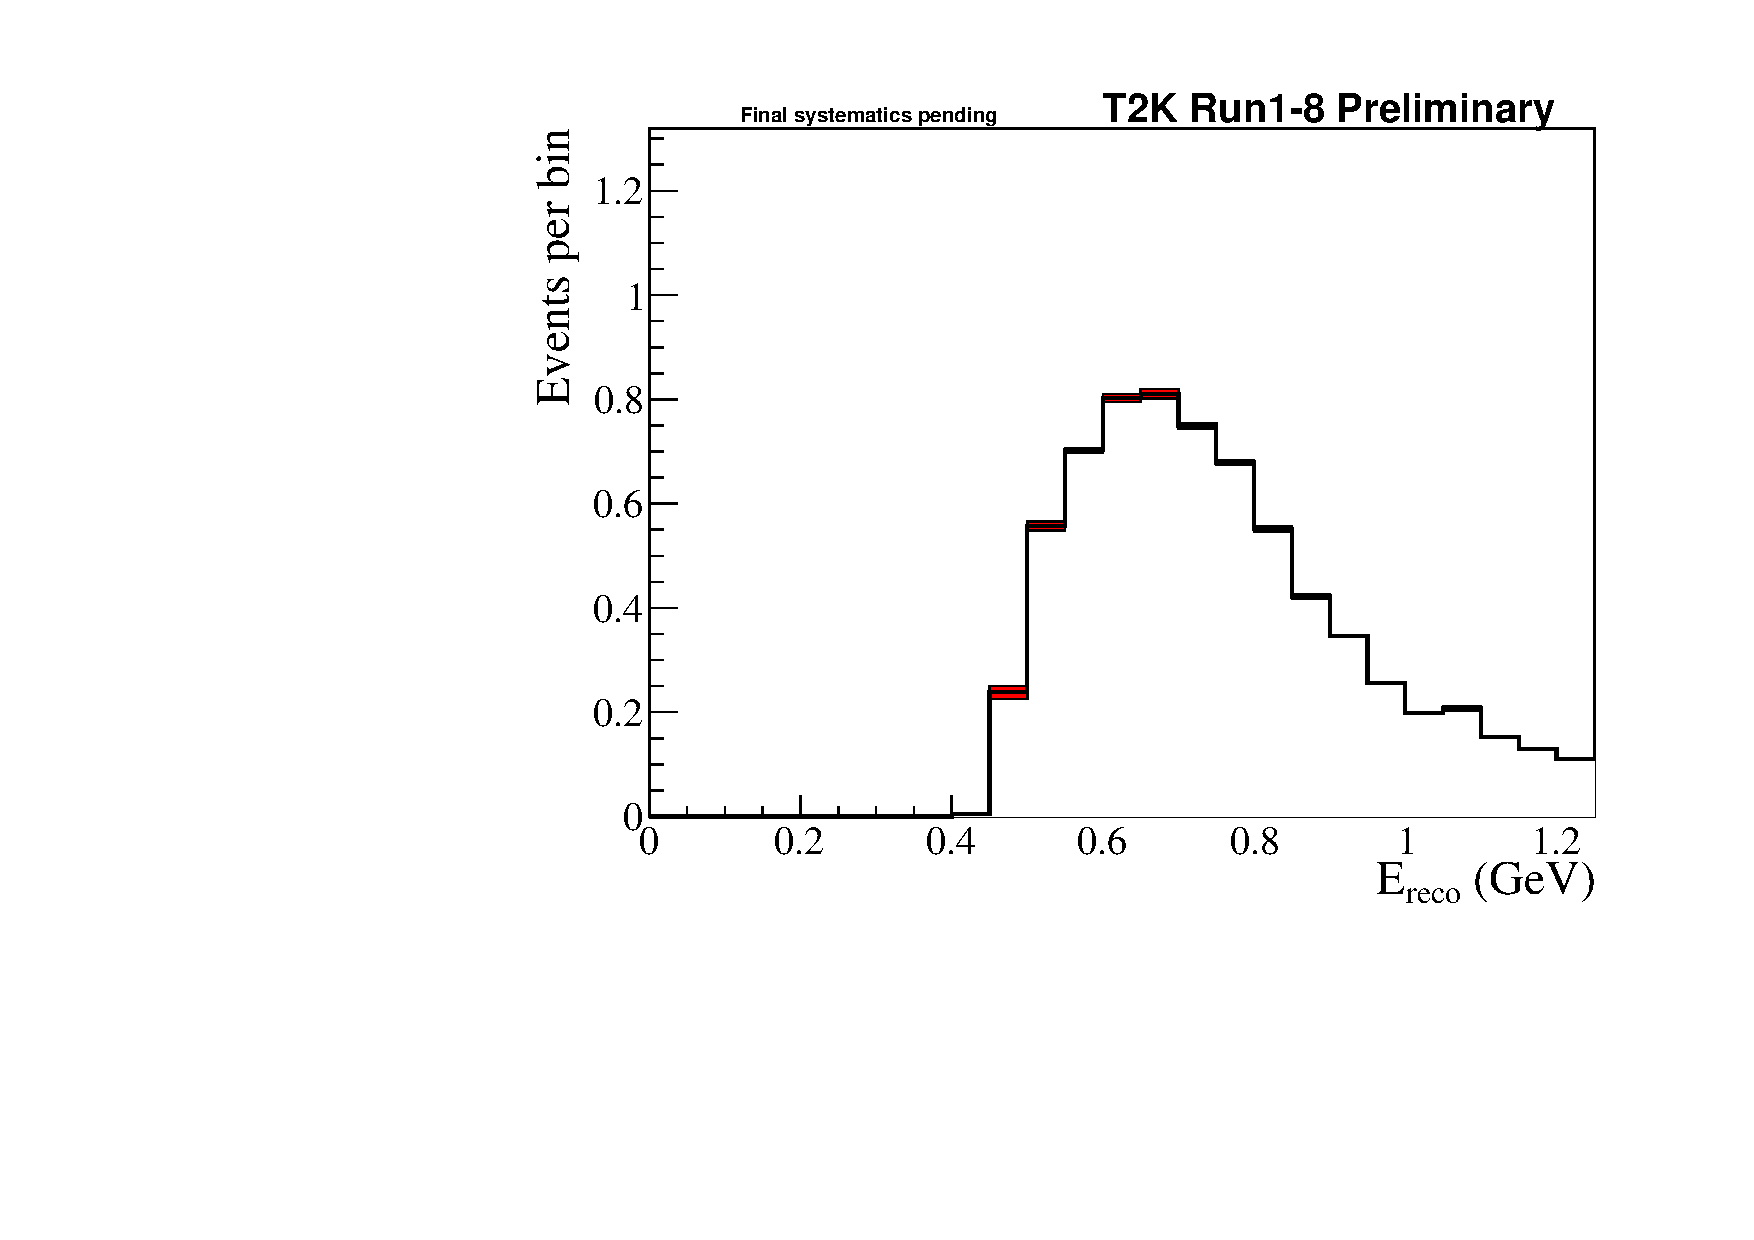
\includegraphics[width=0.9\textwidth]{systematics/envelopes/sk_errors/sk_error_table_MultiRe_xsec_ncoth_envelope}
		\caption{\nueCConepi-like, neutrino mode}
	\end{subfigure}
	\begin{subfigure}[b]{0.49\textwidth}
		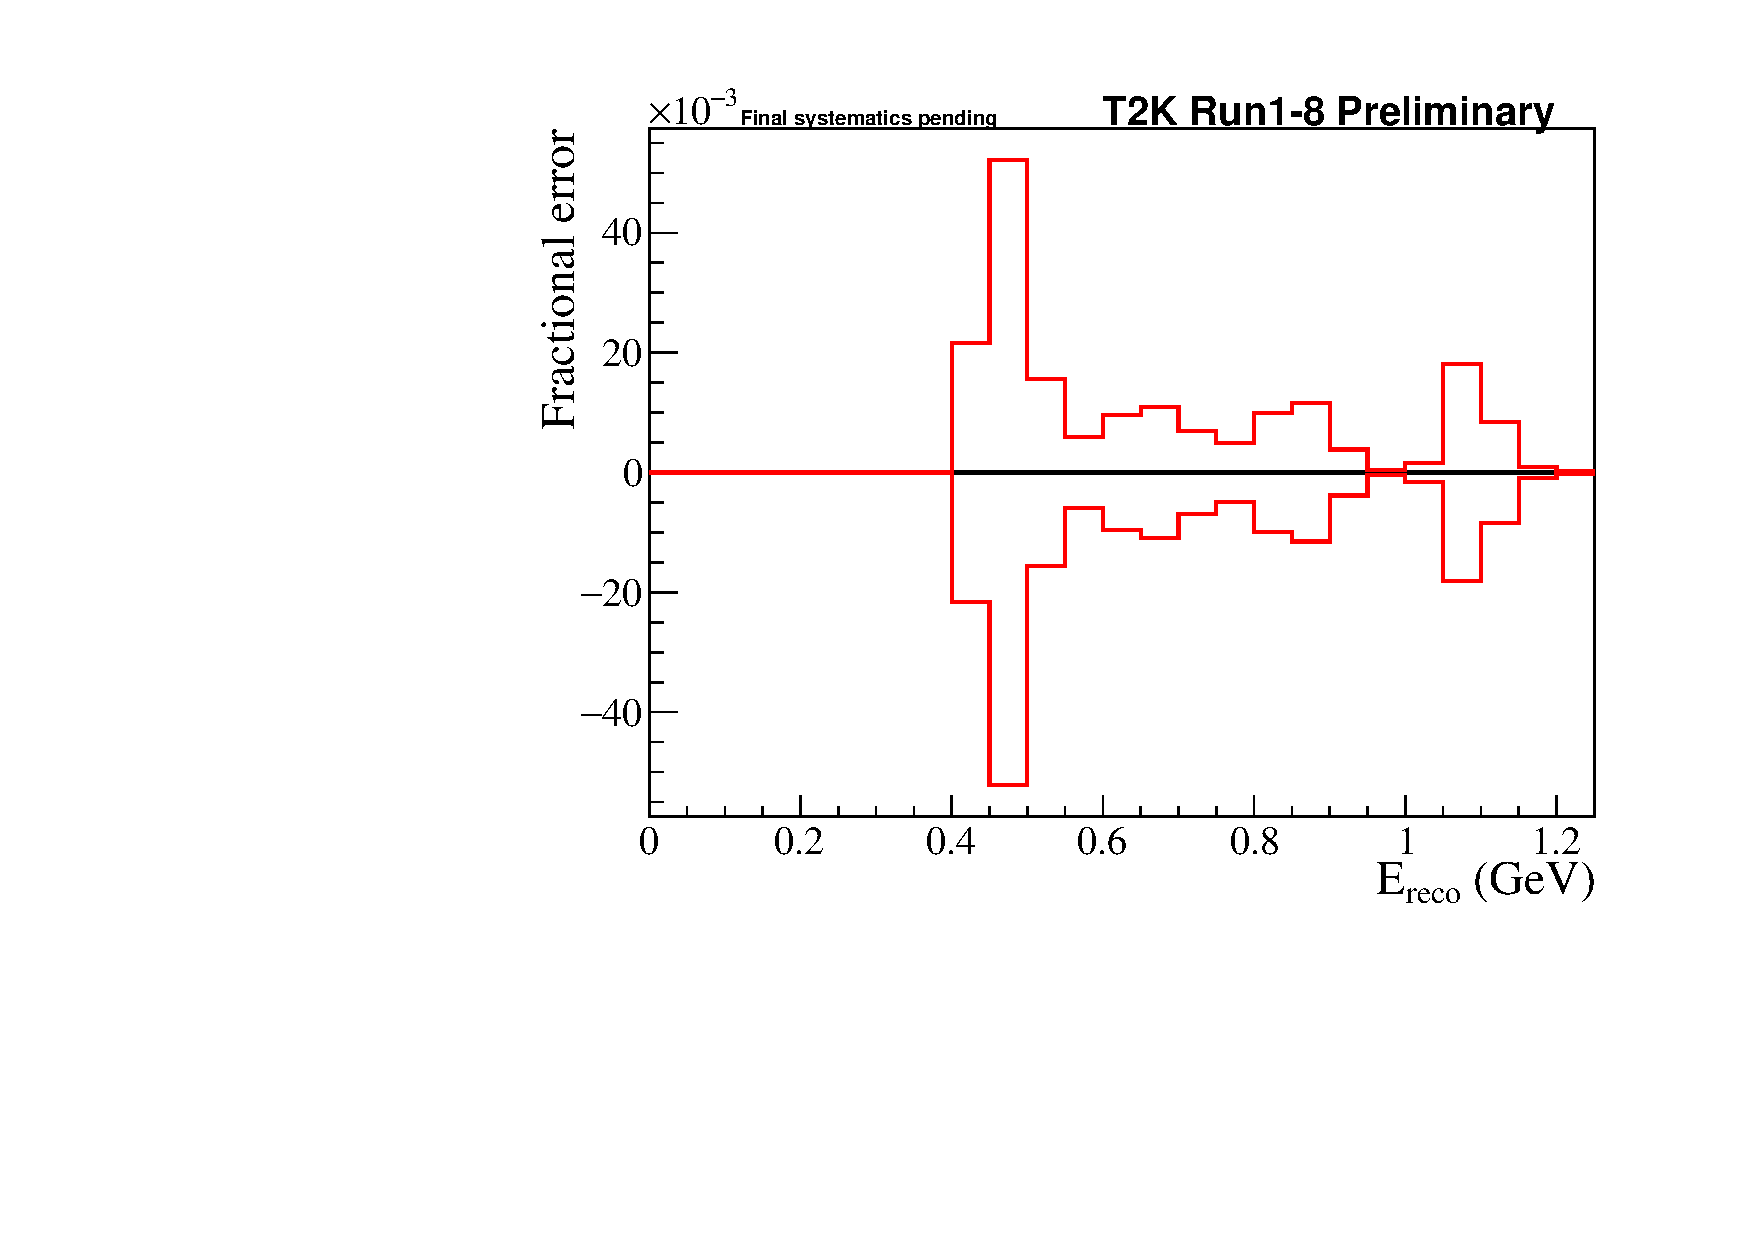
\includegraphics[width=0.9\textwidth]{systematics/envelopes/sk_errors/sk_error_table_MultiRe_xsec_ncoth_envelope_fractional}
		\caption{\nueCConepi-like, neutrino mode}
	\end{subfigure}
	\caption {
		Error envelopes (left) and fractional errors (right) for the reconstructed neutrino energy spectrum for the unconstrained NCother systematic parameters. \num{1e4} toys are generated for the Asimov data set A with randomized systematic parameters with correlations taken into account.
	}
	\label{fig:sk_envelopes_xsec_ncoth}
\end{figure*}
\clearpage

\begin{figure*}
	\center
	\begin{subfigure}[b]{0.49\textwidth}
		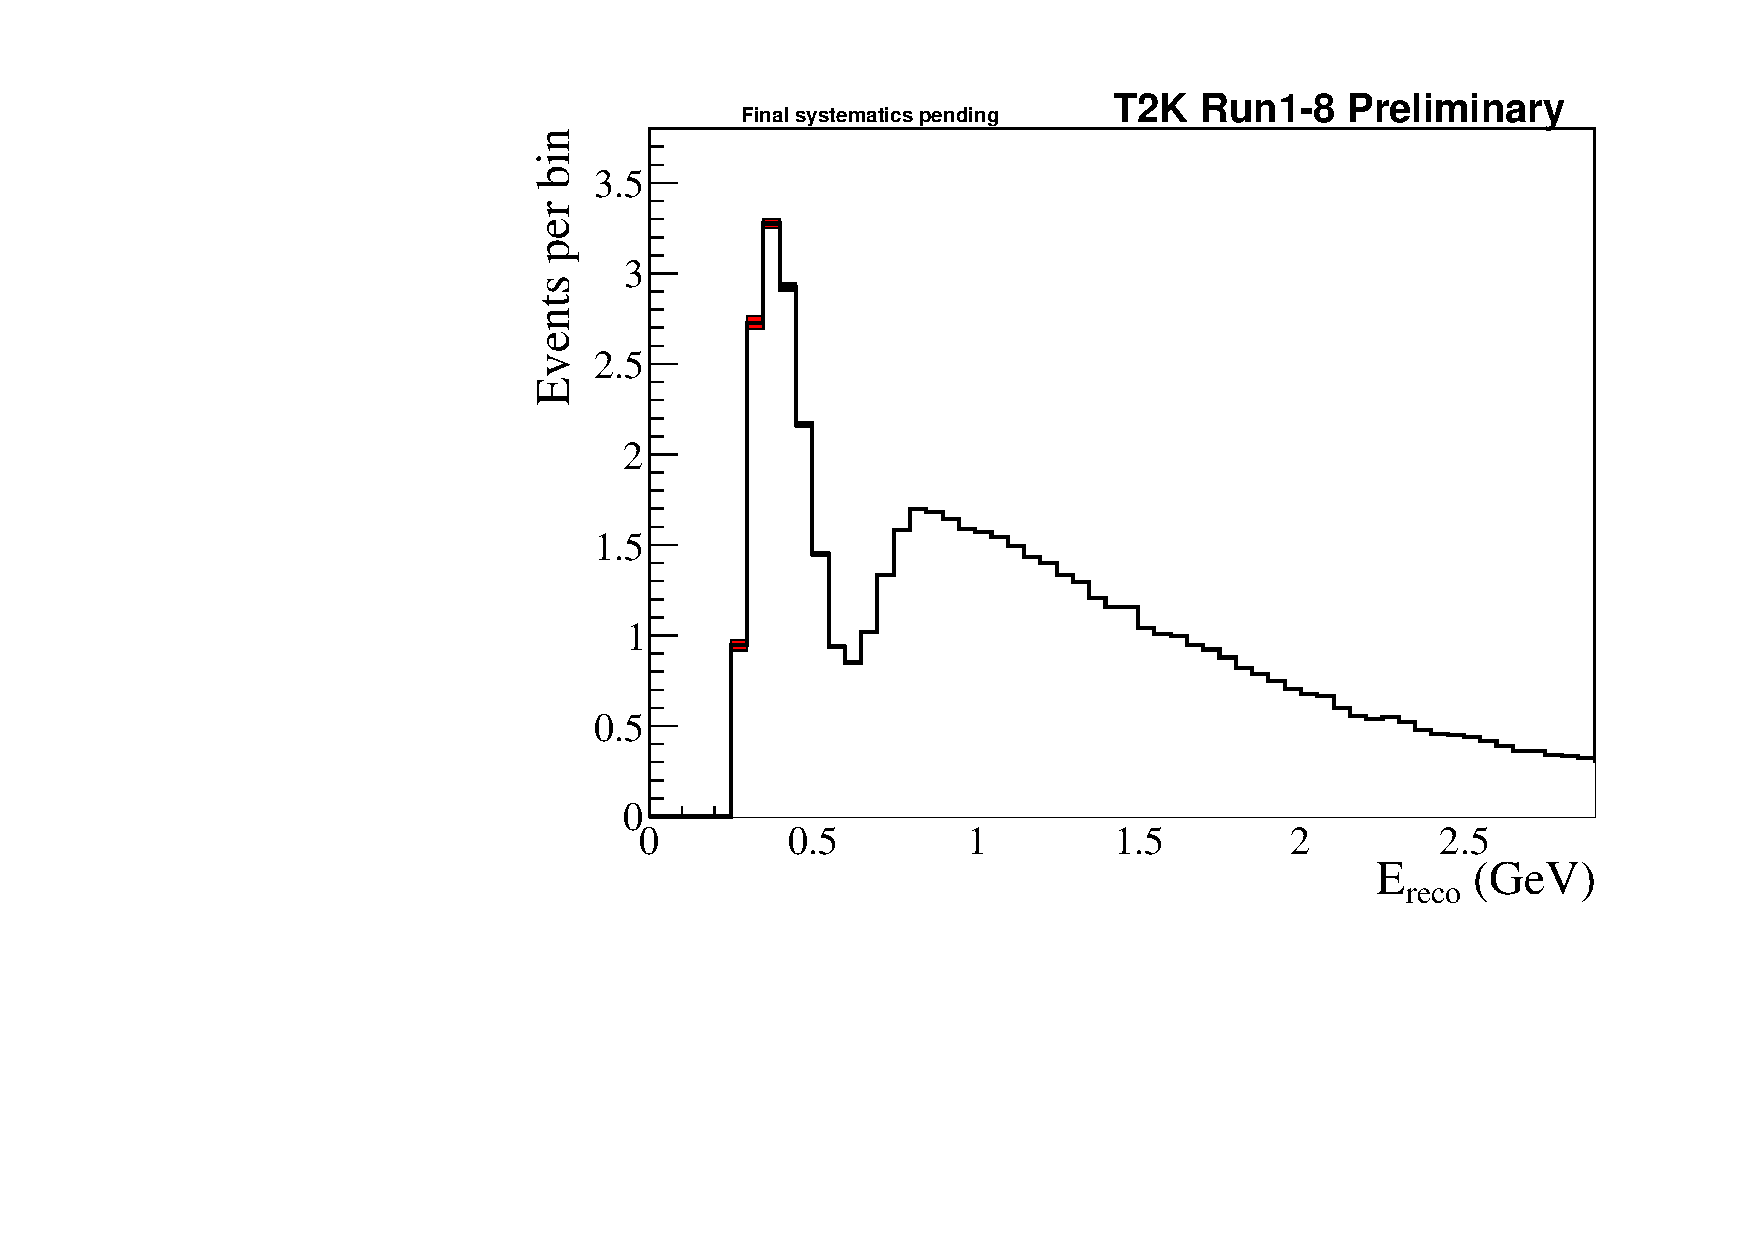
\includegraphics[width=0.9\textwidth]{systematics/envelopes/sk_errors/sk_error_table_RHC1Rmu_xsec_ncoth_envelope}
		\caption{Muon-like, antineutrino mode}
	\end{subfigure}
	\begin{subfigure}[b]{0.49\textwidth}
		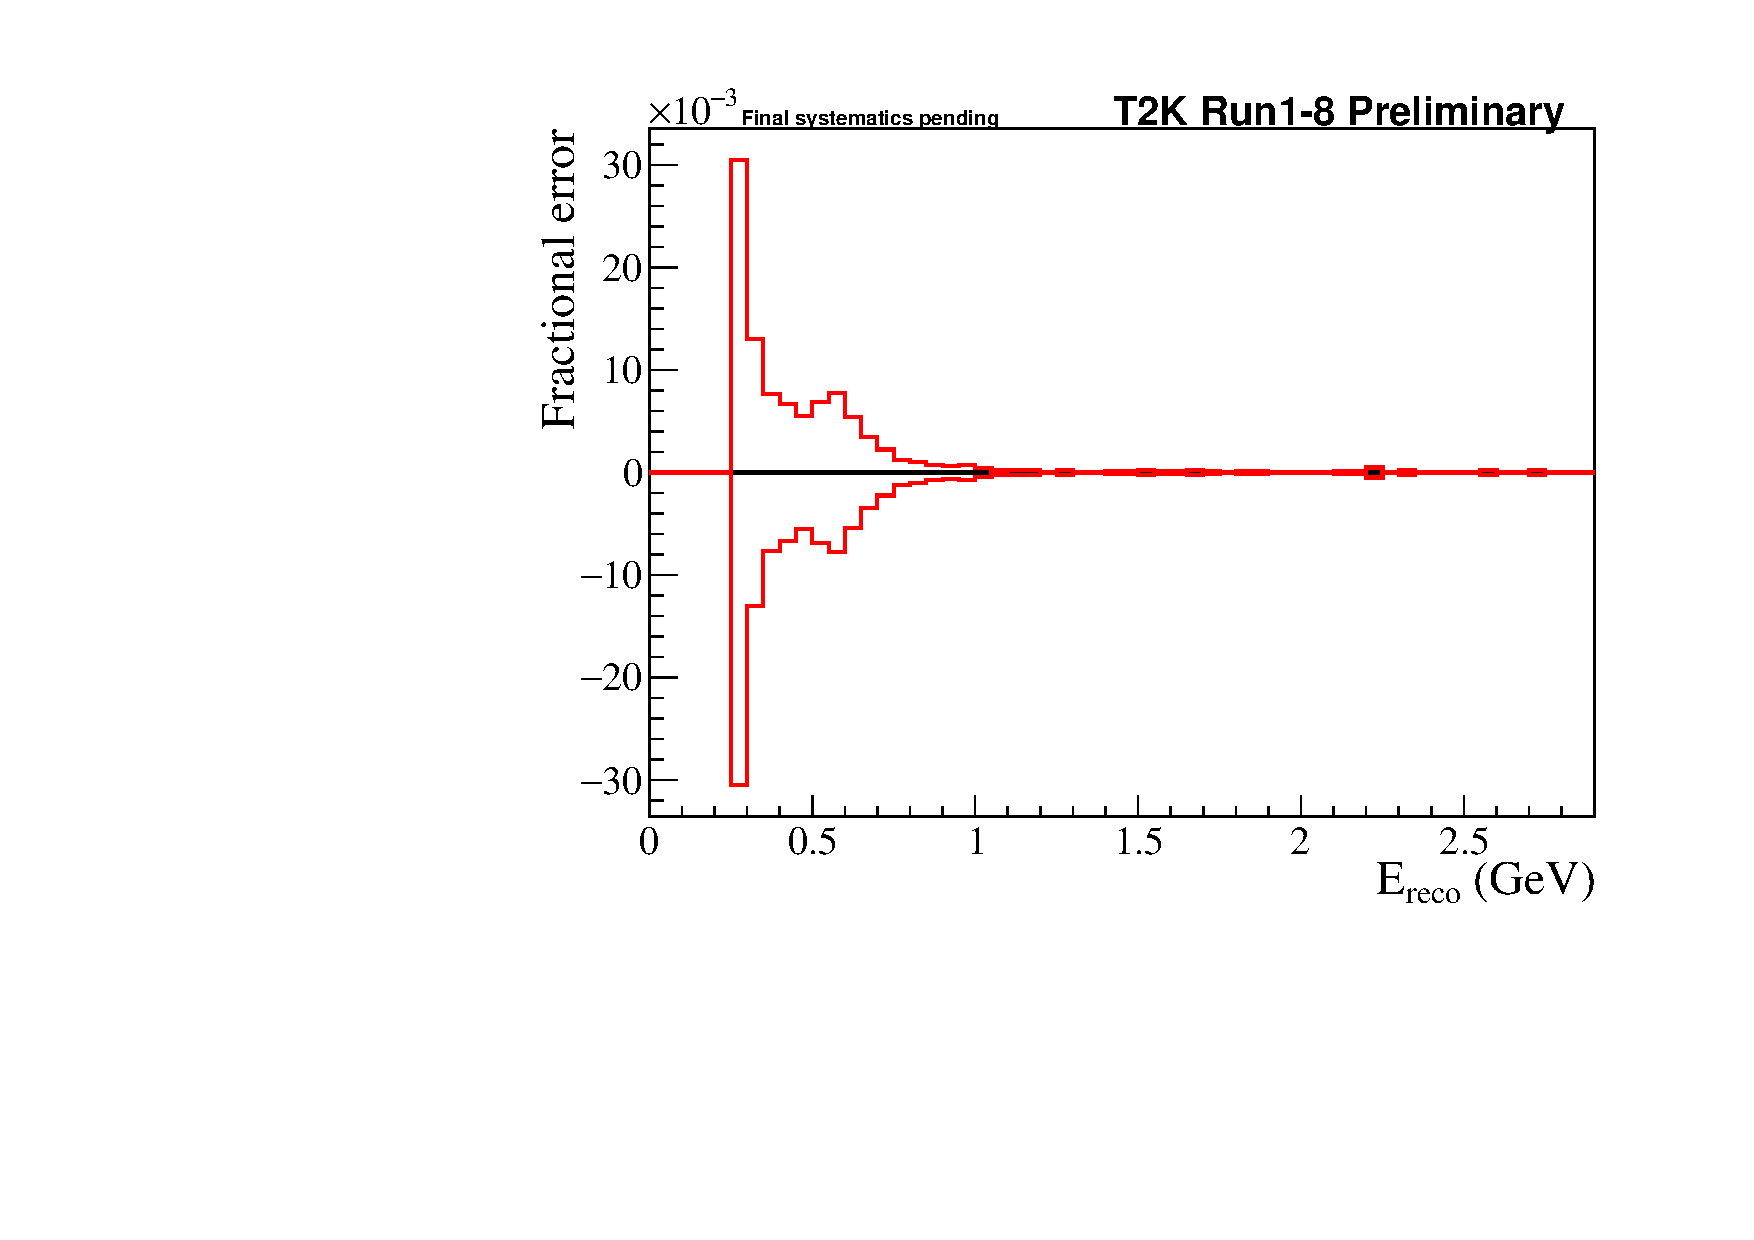
\includegraphics[width=0.9\textwidth]{systematics/envelopes/sk_errors/sk_error_table_RHC1Rmu_xsec_ncoth_envelope_fractional}
		\caption{Muon-like, antineutrino mode}
	\end{subfigure}
	\begin{subfigure}[b]{0.49\textwidth}
		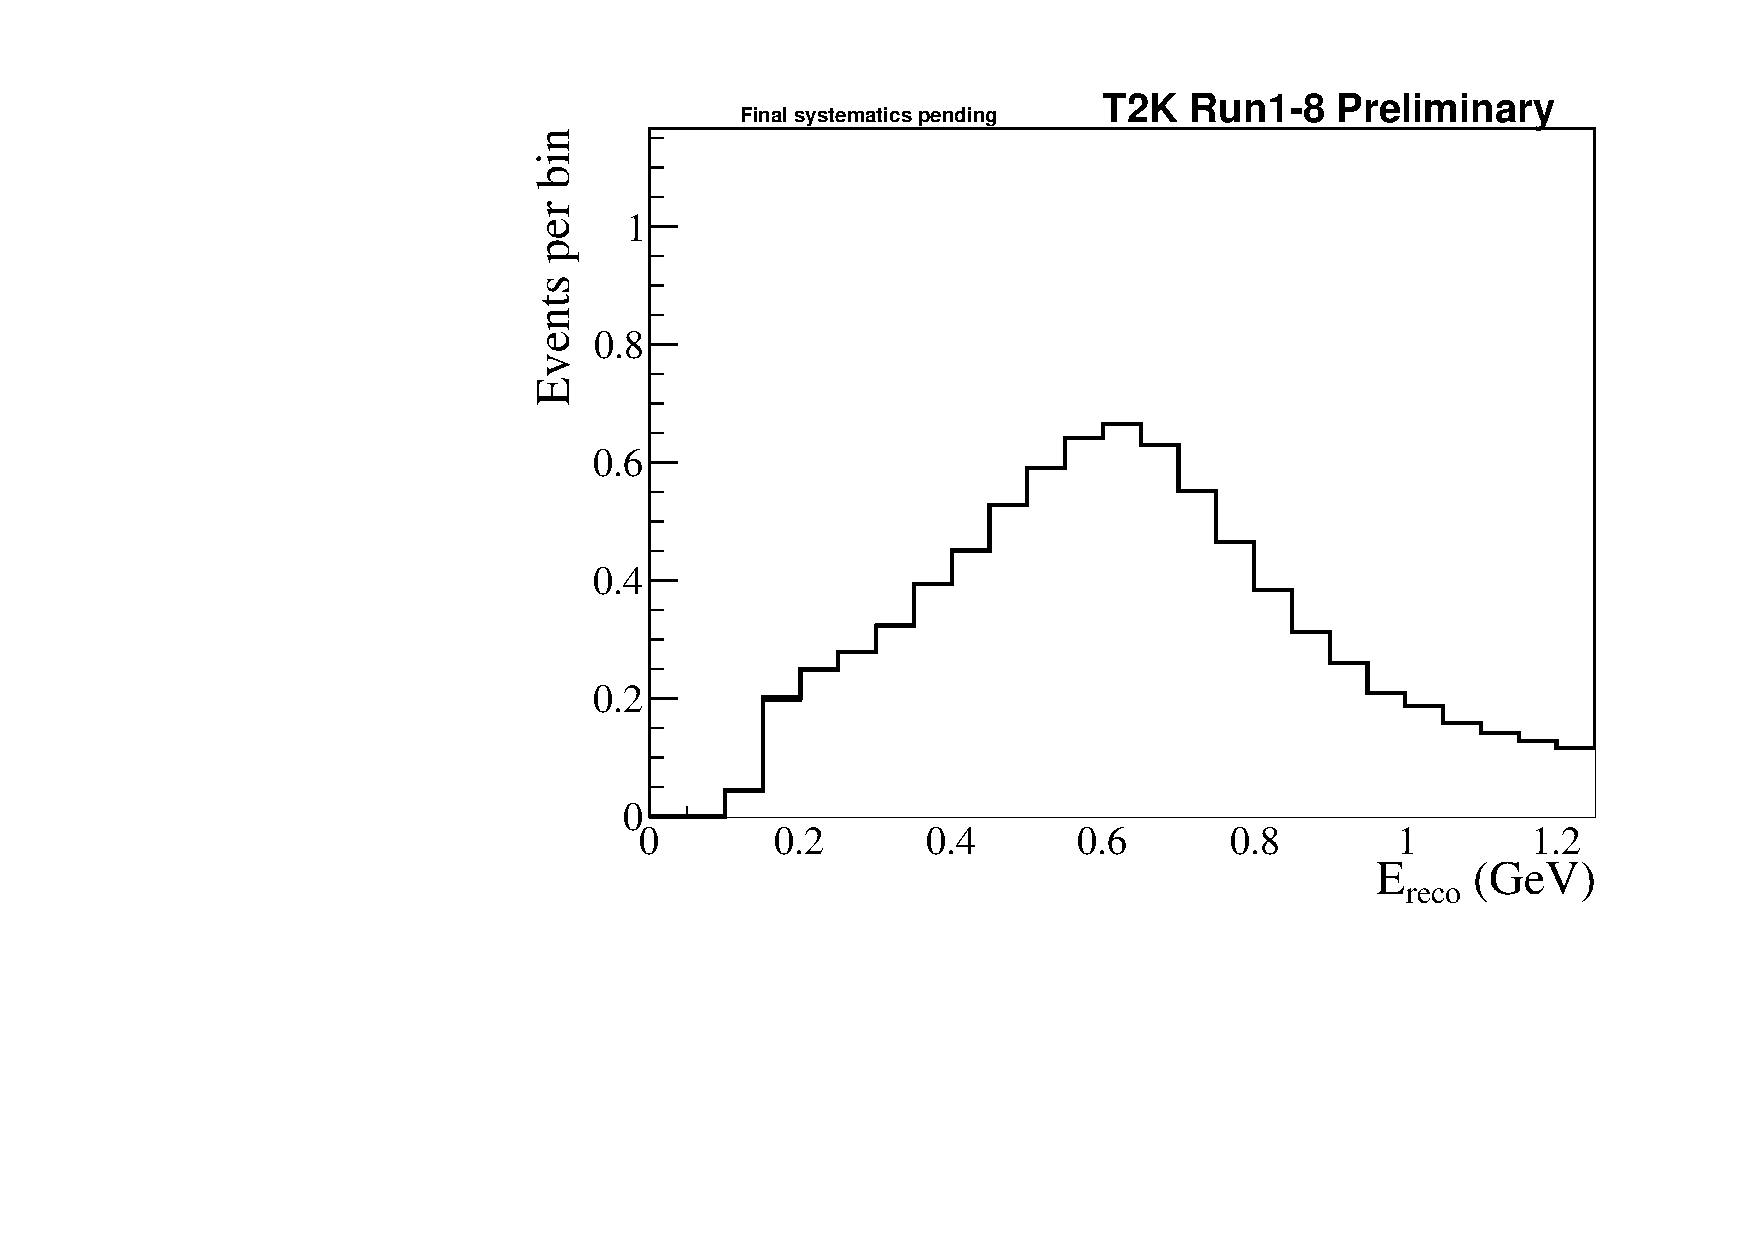
\includegraphics[width=0.9\textwidth]{systematics/envelopes/sk_errors/sk_error_table_RHC1Re_xsec_ncoth_envelope}
		\caption{Electron-like antineutrino mode}
	\end{subfigure}
	\begin{subfigure}[b]{0.49\textwidth}
		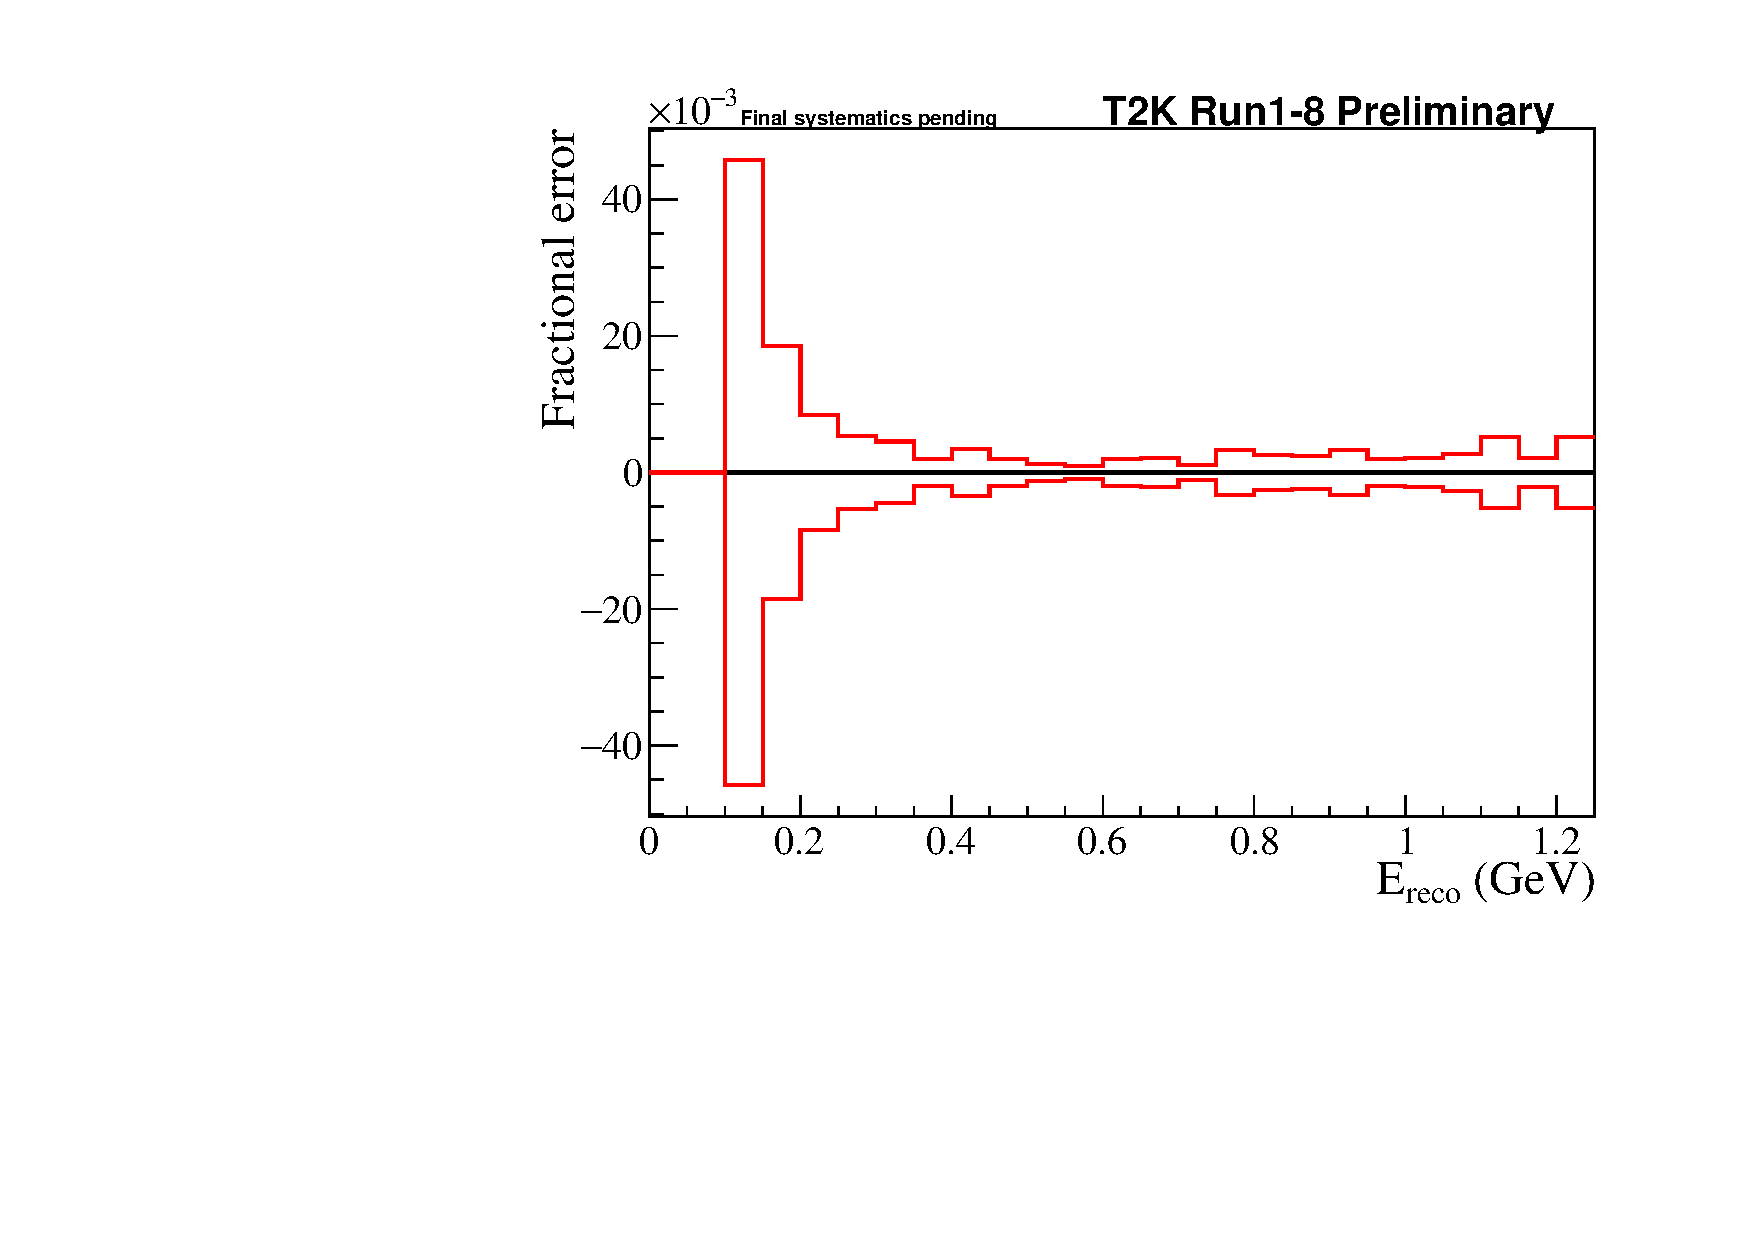
\includegraphics[width=0.9\textwidth]{systematics/envelopes/sk_errors/sk_error_table_RHC1Re_xsec_ncoth_envelope_fractional}
		\caption{Electron-like antineutrino mode}
	\end{subfigure}
	\caption {
		Error envelopes (left) and fractional errors (right) for the reconstructed neutrino energy spectrum for the unconstrained NCother systematic parameters. \num{1e4} toys are generated for the Asimov data set A with randomized systematic parameters with correlations taken into account.
	}
	\label{fig:sk_envelopes_xsec_ncoth_b}
\end{figure*}
\clearpage

\clearpage


%..................

%%% Local Variables:
%%% mode: latex
%%% TeX-master: "../TN327"
%%% End:
